\cotefile{10}
\scanpage{33}
\mspage{\handwritten{1}}
% archive sheet number: 32

\uline{10. Passage à la limite projective dans les préschémas en groupes et les préschémas à groupe d'opérateurs.}

\margin{\handwritten{\figure{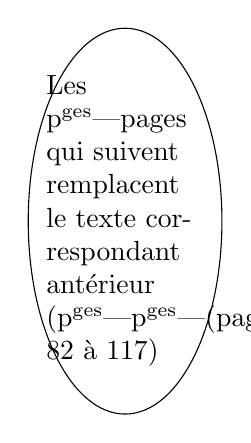
\begin{tikzpicture}
\node[text width=2cm,align=left,inner sep=2pt] at (0,0) {Les \unsure{p\textsuperscript{ges}|pages} qui suivent remplacent le texte correspondant antérieur \unsure{(p\textsuperscript{ges}|p\textsuperscript{ges}|(pages|pages} 82 à 117)};
\draw (0,0) ellipse (1.23 and 2.45);
\end{tikzpicture}}}}
\handwritten{10.}0. Rappelons le résultat essentiel de (EGA IV 8.8) : Etant donnée la situation suivante : $S_o$ un préschéma qu\handwritten{/}asi-compact et quasi-séparé, $I$ un ensemble préordonné filtrant croissant, $(\handwritten{\unsure{\mathscr{A}|\mathcal{A}}}_i)_{i\handwritten{\in}I}$ un système inductif de $\handwritten{\mathcal{O}}_{S_o}$-Algèbres commutatives quasi-cohérentes, $\handwritten{\mathscr{A}}=\underset{\handwritten{\longrightarrow}}{\lim}\handwritten{\mathscr{A}}_i$, $S_i=\operatorname{Spec}\handwritten{\mathscr{A}}_i$ pour $i\handwritten{\in}I$, et $S=\operatorname{Spec}\handwritten{\mathscr{A}}$, \handwritten{a}lors la catégorie des $S$-préschémas de présentation finie est déterminée à équivalence près par la donnée des catégories des $S_i$-préschémas de présentation finie, des foncteurs \inserted{entre ces catégories} $\handwritten{\rho}_{ij}:X_i\handwritten{\rightsquigarrow}X_i\times_{S_i}S_j$ \deleted{\unsure{,}} pour $i\handwritten{\leqq}j$, et des isomorphismes de transitivité $\handwritten{\rho}_{jk}\mathbin{\unsure{o|\circ}}\handwritten{\rho}_{ij}\handwritten{\xrightarrow{\sim}\rho}_{ik}$. \deleted{Plus précisément,} \handwritten{Précisons.}

\margin{\handwritten{\figure{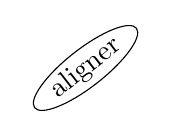
\begin{tikzpicture}
\node[rotate=38,inner sep=1pt] at (0,0) {aligner};
\draw[rotate=38] (0,0) ellipse (.82 and .24);
\end{tikzpicture}}\quad )\quad )}}
Etant donné $j\handwritten{\in}I$, et un $S_j$-préschéma de présentation finie $X_j$, nous poserons,pour tout $i\handwritten{\in}I$ tel que $j\handwritten{\leqq}i$, $X_i=X_j\handwritten{\times}_{S_j}S_i$, et $X=X_j\handwritten{\times}_{S_j}S$. Alors :\inserted{\handwritten{(EGA \uline{IV} 8.8.2)}}\handwritten{\unsure{;|:}}\margin{\handwritten{(}}

\uline{i) Etant donné $j\handwritten{\in}I$, et deux $S_j$-préschémas de présentation finie $X_j$ et $Y_j$, l'application canonique de $\underset{i\handwritten{\geqslant}j}{\underset{\handwritten{\longrightarrow}}{\lim}}\operatorname{Hom} S_i(X_i,Y_i)$ dans $\operatorname{Hom}(X,Y)$ est bijective}\margin{\handwritten{(}}

\uline{ii) Pour tout $S$-préschéma de présentation finie $X$, il existe un indice $j\handwritten{\in}I$, \deleted{et} un $S_j$-préschéma de présentation finie $X_j$ et un $S$-isomorphisme $X\handwritten{\xrightarrow{\sim}}X_j\handwritten{\times}_{S_j}S$.}

On en conclut (EGA IV 8.8.3) que, chaque fois qu'on aura un diagramme $D$ portant sur un nombre fini d'objets et de flèches de la catégorie des $S$-préschémas de présentation finie, on peut trouver un indice $i\handwritten{\in}I$ et un diagramme $D_i$ dans la catégorie des $S_i$-préschémas de présentation finie, tels que le diagramme $D$ provienne à isomorphisme près du diagramme $D_i$ par le changement de base $S\handwritten{\longrightarrow}S_i$. On peut même trouver $i$ et $D_i$ tels que tout carré cartésien de $D$ provienne d'un carré cartésien de $D_i$.

\handwritten{10.1.} De plus, un grand nombre de propriétés \deleted{de} courantes pour un morphisme, stables par changement de base, possèdent la propriété suivante ; étant donné un indice $j\handwritten{\in}I$ deu\deleted{s}\inserted{\handwritten{x}} $S_j$-préschémas de présentation finie $X_j$ et $Y_j$ et un $S_j$-morphisme $u_j:X_j\handwritten{\longrightarrow}Y_j$, pour que $u=u_j\handwritten{\times}_{S_j}S$ ait la propriété $\handwritten{\mathbb{P}}$, il faut et il suffit qu'il existe un indice $i\handwritten{\in}I$ tel que $j\handwritten{\leqq}i$ et que $u_i=u_j\handwritten{\times}_{S_j}S_i$ ait la propriété $\handwritten{\mathbb{P}}$. Il en est ainsi dans le cas où $\handwritten{\mathbb{P}}$ est \deleted{la}\inserted{\handwritten{l'une des}} propriété\inserted{\handwritten{s}}\inserted{\handwritten{suivantes}} pour un morphisme:\deleted{\unsure{d'}}être séparé, surjectif, radiciel, affine, quasi-affine, fini, quasi-fini, propre, projectif, quasi-projectif, un isomor%
\scanpage{34}%
\mspage{\handwritten{2}}%
% archive sheet number: 33
phisme, un monomorphisme, une immersion, une immersion ouverte, une immersion fermée, lisse, non ramifié ou étale (EGA IV 8.10.5, 11.2.6 et 17.7.6). Remarquons qu'il en est encore ainsi \deleted{\unsure{par|pour}} \uline{dans le cas où $\handwritten{\mathbb{P}}$ est la propriété d'être couvrant pour la topologie \handwritten{\unsure{/|f}}fidèlement plate localement de présentation finie} (notée fppf); en effet, étant donnés deux $S$-préschémas de présentation finie $X$ et $Y$, et un \deleted{morphisme}\inserted{$S$-morphisme} $u:X\handwritten{\longrightarrow}Y$, il résulte de (Exp. IV 6.3.1 (i))\deleted{,} que, pour que $u$ soit couvrant pour la topologie fppf, il faut et il suffit qu'il existe un $S$-préschéma $Z$ et un $S$-morphisme $v:Z\handwritten{\longrightarrow}Y$ fidèlement plat et de présentation finie qui se factorise à travers $u$.

Le but de ce numéro est \deleted{d'étendre}\inserted{\handwritten{de donner des variantes de}} ce genre de résultats \deleted{à}\inserted{\handwritten{pour}} la catégorie des $S$-groupes de présentation finie, \deleted{et à} celle des $S$-préschémas à groupe d'opérateurs, et \deleted{à}\inserted{\handwritten{pour}} certaines propriétés pour des monomorphismes de groupes (être invariant, central, à faisceau quotient inversible, etc ...).

Les deux résultats préliminaires de ce type sont les suivants :

\uline{10.\handwritten{2}.} \deleted{\unsure{a)}} \uline{Dans la situation rappelée au début de (10.0), soient \deleted{\unsure{pour}} $j\handwritten{\in}I$, $G_j$ et $H_j$ deux $S_j$-groupes de présentation finie; posons, pour tout $i\handwritten{\in}I$ tel que $j\handwritten{\leqq}i$, $G_i=G_j\handwritten{\times}_{S_j}S_i$, $G=G_j\handwritten{\times}_{S_j}S$, et définissons de même $\deleted{\unsure{G}}$ $H_i$ et $H$. Alors l'application canonique de $\underset{i\handwritten{\geqslant}j}{\underset{\handwritten{\longrightarrow}}{\lim}}\operatorname{Hom}_{\unsure{S|\mathbb{S}}_i\text{-gr.}}(G_i,H_i)$ dans $\operatorname{Hom}_{S\text{-gr.}}(G,H)$ est bijective.}

\uline{10.\handwritten{3}.} \deleted{\unsure{b)}} \uline{Dans la situation rappelée au début de (10.0), soit $G$ un $S$-groupe de présentation finie; alors il existe un indice $j\handwritten{\in}I$, \deleted{et} un $S_j$-groupe de présentation \deleted{f} finie $G_j$, et un \deleted{\illegible{1}} $S$-isomorphisme de groupes de $G$ sur $G_j\handwritten{\times}_{S_j}S$.}

Les assertions (10.\handwritten{\unsure{2|1}}) et (10.\handwritten{3}) sont des conséquences faciles de \deleted{(EGA IV 8.8.2 et 8.8.3)}\inserted{\handwritten{(10.0) et (10.1),}} compte tenu de l'interprétation de la structure de $S$-groupe donnée en (EGA $0_{\mathrm{III}}$ 8.2.5 et 8.2.6).

% Cancelled text visible through the pasted lower strip. The last line is
% read after vertical reflection; the other lines remain in the scan orientation.
\deleted{\unsure{10.4. Soit} $\unsure{\mathbb{P}}$ \unsure{l'une des propriétés} \illegible{5} \unsure{de préschémas en groupes} \illegible{1}}

\deleted{\unsure{(ii)|(i)} être un monomorphisme, \unsure{(i.e.} $\unsure{G}$ \illegible{7} $\unsure{H}$\unsure{)}}

\deleted{\unsure{(iii)|(ii)} être une immersion \unsure{(i.e.} $\unsure{G}$ \unsure{est un sous-préschéma en groupes de} $\unsure{H}$\unsure{)}}

\deleted{\unsure{(iv)|(iii)} être une immersion fermée \unsure{(i.e.} $G$ est un sous-préschéma en groupes fermé}

\scanpage{35}
\mspage{\handwritten{3}}
% archive sheet number: 34

\deleted{fermé de $H$),}

\deleted{\uline{\unsure{i)|v)} être un monomorphisme central (6.6),}}

\deleted{\uline{vi) être un monomorphisme invariant (6.6).}}

\inserted{\handwritten{10.4.}} \uline{Soient $j\handwritten{\in}I$, $G_j$ et $H_j$ deux $S_j$-groupes de présentation finie, et $u_j:G_j\handwritten{\longrightarrow}H_j$ un morphisme de $S_j$-groupes. Pour que $u=u_j\handwritten{\times}_{S_j}S$ \deleted{ait la propriété $\handwritten{\mathbb{P}}$} }\inserted{\handwritten{\figure{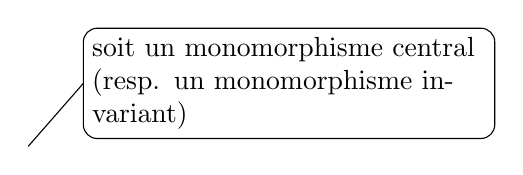
\begin{tikzpicture}
\node[align=left,text width=5cm,inner sep=3pt] (n) at (0,0) {soit un monomorphisme central (resp. un monomorphisme invariant)};
\draw[rounded corners=5pt] (n.south west) rectangle (n.north east);
\draw (n.west) -- ++(-.7,-.8);
\end{tikzpicture}}}}\uline{, il faut et il suffit qu'il existe $i\handwritten{\in}I$, $i\handwritten{\geqslant}j$ tel que $u_i=u_j\handwritten{\times}_{S_j}S_i$ ait la \inserted{\handwritten{même}}propriété $\deleted{\handwritten{\unsure{\mathbb{P}}}}$.}

\deleted{Les assertions (i) à (iv) résultent de (EGA 8.10.5). Les assertions (v) et (vi) sont}\inserted{\handwritten{C'est}} une conséquence immédiate de \deleted{(EGA 8.8.2 et 8.8.3)}\inserted{\handwritten{(10.0) et (10.1),}} compte tenu de la caractérisation donnée en (6.7) des monomorphismes de groupes centraux et invariants.

\inserted{\handwritten{\uline{Corollaire}}} \uuline{10.5.} \uline{Soit $j\handwritten{\in}I$, et soit $G_j$ un $S_j$-groupe de présentation finie. Pour que $G=G_j\handwritten{\times}_{S_j}S$ soit abélien, il faut et il suffit qu'il existe $i\handwritten{\in}I$, $i\handwritten{\geqslant}j$, tel que $G_i=G_j\handwritten{\times}_{S_j}\deleted{\unsure{H}_{\unsure{j|i}}}\inserted{S_i}$ soit abélien.}

En effet, il revient au même de dire qu'un $S$-groupe est abélien, ou que, considéré comme sous-préschéma en groupes de lui-même, il est central.

\uline{Proposition 10.6.}- \uline{Dans la s\unsure{i|à}tuation rappelée au début de (10.0), soient $j\handwritten{\in}I$, $G_j$ un $S_j$-groupe de présentation finie, $G'_j$ un sous-préschéma en groupes de $G_j$ plat et de présentation finie sur $S_j$. Pour que $G_j\handwritten{\times}_{S_j}S/G'_j\handwritten{\times}_{S_j}S$ soit représentable (pour la topologie fpqc), il faut et il suffit qu'il existe $i\handwritten{\in}I$, $i\handwritten{\geqslant}j$, tel que $G_j\handwritten{\times}_{S_j}S_i/G'_j\handwritten{\times}_{S_j}S_i$ soit représentable.}

C'est une conséquence \deleted{p}du lemme plus général suivant :

\margin{\handwritten{$\mathbb{T}$}}
\uline{Lemme 10.7.}- \uline{Soit $\handwritten{\mathbb{T}}$ la topologie fppf ou fpqc; soient $j\handwritten{\in}I$, $X_j$ un $S_j$-préschéma de}
\scanpage{36}
\mspage{\handwritten{4}}
% archive sheet number: 35
\uline{présentation finie, et $R_j$ une relation d'équivalence sur $X_j$ définie par un $S_j$-monomorphisme $v_j:R_j\handwritten{\longrightarrow}X_j\handwritten{\times}_{S_j}X_j$ tel que le morphisme $\operatorname{pr}_{1,j}\mathbin{\unsure{o|\circ}} v_j:R_j\handwritten{\longrightarrow}X_j$ déduit de $v_j$ par composition avec la première projection $X_j\handwritten{\times}_{S_j}X_j\handwritten{\longrightarrow}X_j$ soit plat et de présentation finie. Alors, pour que le faisceau quotient $X_j\handwritten{\times}_{S_j}S/R_j\handwritten{\times}_{S_j}S$ pour la topologie $\handwritten{\mathbb{T}}$ soit représentable, il faut et il suffit qu'il existe $i\handwritten{\in}I$, $i\handwritten{\geqslant}j$, le faisceau quotient $X_j\handwritten{\times}_{S_j}S_i/R_j{}_{S_j}S_i$ pour la topologie $\handwritten{\mathbb{T}}$ soit représentable.}

Compte tenu des énoncés de (EGA IV 8.8.2, 8.8.3, 8.10.5 et 11.2.6) rappelés en (10.0), ce lemme est conséquence\deleted{\unsure{du}} du résultat suivant :

\uline{Lemme 10.8.}- \uline{Soit $\handwritten{\mathbb{T}}$ la topologie fppf ou fpqc ; soient $\deleted{\unsure{j\in I,}}$ $X$ un $S$-préschéma de présentation finie (resp. localement de présentation finie), $R$ une relation d'\handwritten{é}quivalence sur $X$ définie par un monomorphisme $v:R\handwritten{\longrightarrow}X\handwritten{\times}_S X$ tel que $\operatorname{pr}_1\mathbin{o} v$ soit plat et de présentation finie (resp. plat et localement de présentation finie). Alors les conditions suivantes sont équivalentes :}

\uline{(i) Le faisceau quotient $X/R$ pour la topologie $\handwritten{\mathbb{T}}$ est représentable.}

\uline{(ii) il existe un $S$-préschéma de présentation finie (resp. localement de présentation finie ) $Y$ et un morphisme fidèlement plat $p:X\handwritten{\longrightarrow}Y$ tel que le diagramme}

% Diagram objects and labels typed; connecting arrows handwritten.
\diagram{\(\text{(D)}\)\qquad\begin{tikzcd}[ampersand replacement=\&,column sep=large,row sep=large]
R \handwritten{\arrow[r,"\operatorname{pr}_1\mathbin{o} v"]} \handwritten{\arrow[d,"\operatorname{pr}_2\mathbin{o} v"']} \& X \handwritten{\arrow[d,"p"]} \\
X \handwritten{\arrow[r,"p"']} \& X
\end{tikzcd}}

(où $\operatorname{pr}_1$ et $\operatorname{pr}_2$ sont les projections $X\handwritten{\times}_S X\handwritten{\unsure{\substack{\longrightarrow\\[-.6ex]\rightharpoonup}|\rightrightarrows}}X$) \uline{soit cartésien.}

Notons d'abord que d'après (Exp. IV 3.3.2 et 4.4.3), pour que le faisceau $X/R$ \deleted{\illegible{1}} pour la topologie $\handwritten{\mathbb{T}}$ soit représentable par $Y$, il faut et il suffit que le diagramme (D) soit cartésien et que $p$ soit couvrant pour la topologie $\handwritten{\mathbb{T}}$.

Montrons que i) entraîne ii). L'hypothèse (i) implique que le diagramme (D) est cartésien, donc que $\operatorname{pr}_1\mathbin{o} v$ se déduit de $p$ par changement de base par $p$, et que $p$ est
\scanpage{37}
\mspage{\handwritten{5}}
% archive sheet number: 36
est couvrant pour la topologie fpqc. Puisque $\operatorname{pr}_1\mathbin{\unsure{o|\circ}} v$ est fidèlement plat et de présentation finie, (resp. fidèlement plat et localement \deleted{pd}\inserted{de} présentation finie), il en est de même de $p$ (EGA IV 2.7.1), et comme $X$ est de présentation finie (resp. localement de présentation finie) sur $S$, il en est de même de $Y$ (EGA IV 17.7.4).

Montrons que ii) entraîne i). Il suffit de montrer que $p$ est couvrant pour la topologie fppf; or $p$ est fidèlement plat par hypothèse, et localement de présentation finie, puisque $X$ et $Y$ sont localement de présentation finie sur $S$.

\uline{10.9.}- \uline{Dans la situation rappelée au début de (10.0), soient $j\handwritten{\in}I$, et $G_j$ un $S_j$-groupe de présentation finie. Pour que $G^o=(G_j\handwritten{\times}_{S_j}S)^o$ soit représentable, il faut et il suffit qu'il existe \deleted{\unsure{un}} $i\handwritten{\in}I$, $i\handwritten{\geqslant}j$, tel que $(G_i)^o=(G_j\handwritten{\times}_{S_j}S_i)^o$ soit représentable.}

La condition est suffisante (3.3).

Montrons que la condition est nécessaire. \deleted{Alors}\inserted{\handwritten{En effet,}} $G^o$ est de présentation finie sur $S$ et ouvert dans $G$ (3.9). D'après (10.0), il existe $i\handwritten{\in}I$, $i\handwritten{\geqslant}j$, et un sous-préschéma en groupes ouvert $G_i^o$ de $G_i$ tel que $G_i^o\handwritten{\times}_{S_i}S=G^o$. Le morphisme structural $G^o\handwritten{\longrightarrow}S$ est connexe (i.e. à fibres géométriquement connexes)(Exp. $\mathrm{VI}_A$ 2.1.1). Alors, (EGA IV 9.3.3 et 9.7.7), quitte à augmenter $i$, on peut supposer que le morphisme structural $G_i^o\handwritten{\longrightarrow}S$ est connexe, donc que l'espace sous-jacent à $G_i^o$ n'est autre que \uline{$\handwritten{(}G_i^{\deleted{o}}\handwritten{)^o}$} (3.10.1), donc que $G_i^o$ représente $(G_i)^o$.

\uline{10.10.} \uuline{Rappelons de\deleted{\unsure{v|y}}\inserted{\handwritten{u}}x cas particuliers très utiles de la situation énoncée en (10.0)}

a) Etant donné un point $x$ d'un préschéma $X$, on pose $S_o=\operatorname{Spec}\handwritten{\mathbb{Z}}$\handwritten{/}et on considère la famille $(S_i)_{i\handwritten{\in}I}$ filtrante décroissante des voisinages \deleted{\unsure{principaux}} ouverts affines de $x$; alors $S=\operatorname{Spec}\handwritten{\mathcal{O}}_{X,x}$. En particulier, si $x$ est le point générique d'un schéma intègre $X$, on trouve $S=\handwritten{\kappa}(x)$.

b) On pose $S_o=\operatorname{Spec}\handwritten{\mathbb{Z}}$, et on considère la famille $(\handwritten{\unsure{\mathscr{A}|\mathcal{A}}}_i)_{i\handwritten{\in}I}$ préordonnée par inclusion des sous-$\handwritten{\mathbb{Z}}$-algèbres de type fini de l'anneau d'un schéma affine $S$.
\scanpage{38}
\mspage{\handwritten{6}}
% archive sheet number: 37

\margin{\handwritten{\figure{
\begin{tikzpicture}[scale=.75]
\node[rotate=25,inner sep=1pt] at (0,0) {intervertir};
\draw[rotate=25] (0,0) ellipse (1.05 and .27);
\end{tikzpicture}}}}
Etant donné que les $\handwritten{\unsure{\mathscr{A}|\mathcal{A}}}_i$ sont des anneaux \deleted{\unsure{pas}} nœ thériens, cela permet dans de nombreux\inserted{\handwritten{cas}} de passer
% The typed words retain their positions; the circles and transposition arrow are handwritten.
\figure{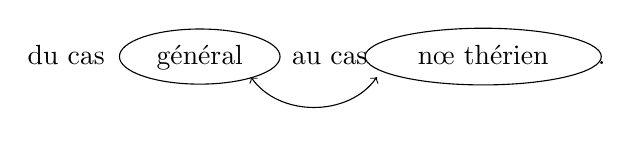
\begin{tikzpicture}
\node[anchor=base east,inner sep=0pt] at (-1.2,0) {du cas};
\node[anchor=base,inner sep=0pt] at (0,0) {général};
\node[anchor=base,inner sep=0pt] at (1.65,0) {au cas};
\node[anchor=base,inner sep=0pt] at (3.6,0) {nœ thérien};
\node[anchor=base west,inner sep=0pt] at (5.05,0) {.};
\handwritten{\draw (0,.10) ellipse (1.02 and .35);
\draw (3.6,.10) ellipse (1.50 and .36);
\draw[<->] (.65,-.16) to[out=-55,in=-125] (2.25,-.16);}
\end{tikzpicture}}

Nous allons maintenant donner deux résultats concernant le cas particulier envisagé en a).

\uline{Proposition 10.11.}- \uline{Soient $S$ un préschéma intègre de point générique $\handwritten{\eta}$, $G$ un $S$-groupe de présentation finie, $X$ un $S$-préschéma de présentation finie, $u$ et $v$ deux $S$-morphismes de $X$ dans $G$, $i:H\handwritten{\longrightarrow}G$ et $j:K\handwritten{\longrightarrow}G$ deux monomorphismes de présentation finie. Alors :}

\uline{(i) il existe un ouvert non vide $S'$ de $S$ tel que si on note $G'$ (resp $H'$, resp. $X'$, resp $u'$, resp $v'$) la restriction de $G$(resp. $H$,resp. $X$, resp. $u$,resp. $v$) au-dessus de l'ouvert $S'$ de $S$, le foncteur\deleted{\unsure{s}} $\underline{\operatorname{Transp}}(u',v')$ (resp. $\underline{\operatorname{Centr}}(u')$, $\underline{\operatorname{Centr}}_{G'}H')$ soit représentable par un sous-$S'$-préschéma fermé de présentation finie $T'_1$ (resp. $C'_1$, resp. $C'_2$) de $G'$.}

\uline{(ii) supposons que $K_{\handwritten{\eta}}$ soit fermé dans $G_{\handwritten{\eta}}$ (ce qui est le cas si $K$ est un sous-$\deleted{p}S$-préschéma en groupes de $G$ (1.4.2)); alors il existe un ouvert non vide $S'$ de $S$ tel que si on note $G'$ (resp. $H'$, resp. $K'$) la restriction de $G$ (resp. $H$, resp. $K$)au-dessus de l'ouvert $S'$ de $S$, le foncteur $\underline{\operatorname{Transp}}_{G'}(H',K')$ (resp. $\underline{\operatorname{Norm}}_{G'}K')$ soit représentable par un sous-$S'$-préschéma fermé de présentation finie $T'_2$ (resp. $N'$) de $G'$.}

\uline{(iii)supposons que $H_{\handwritten{\eta}}$ et $K_{\handwritten{\eta}}$ soient fermés dans $G_{\handwritten{\eta}}$ (ce qui est le cas si $H$ et $K$ sont des sous-préschémas en groupes de $G$ (1.4.2)); alors il existe} \inserted{\handwritten{un ouvert}} \uline{non vide $S'$ de $S$ tel que si on note $G'$ (resp $H'$, resp. $K'$) la restriction de $G$ (resp. $H$, resp. $K$) au-dessus de l'ouvert $S'$ de $S$, le foncteur $\underline{\operatorname{Transpstr}}_{G'}(H',K')$ soit représentable par un sous-$S'$-préschéma fermé de présentation finie de $G'$.}

Puisque $G_{\handwritten{\eta}}$, $X_{\handwritten{\eta}}$, $H_{\handwritten{\eta}}$, $K_{\handwritten{\eta}}$ sont plats sur le corps $\handwritten{\kappa}(\handwritten{\eta})$, et que
\scanpage{39}
\mspage{\handwritten{7}}
% archive sheet number: 38
$G_{\handwritten{\eta}}$ est séparé sur $\handwritten{\kappa}(\handwritten{\eta})$ (\deleted{Exp.} $\mathrm{VI}_A$ 0.2), d'après (10.2,10.10 a),EGA IV 8.8.2 et 8.10.5), il existe un ouvert\inserted{affine} $S'$ de $S$ tel que $G'$ soit un $S'$-groupe de \deleted{type}\inserted{présentation} fini, plat et séparé sur $S'$, et que $X'$, $H'$ et $K'$ soient plats et de présentation finie sur $S'$. Si on suppose $H_{\handwritten{\eta}}$ (resp. $K_{\handwritten{\eta}}$) fermé dans $G_{\handwritten{\eta}}$, on peut choisir $S'$ de sorte que $H'$ (resp. $K'$) soit fermé dans $G'$. D'après (EGA IV 11.3.15), quitte à remplacer $S'$ par un ouvert affine de $S'$, on peut supposer que $G'$, $H'$, $K'$ et $X'$ sont essentiellement libres sur $S'$ (au sens de \deleted{Exp.} VIII (6.1)). Il résulte alors de (\deleted{Exp.} VIII \handwritten{5}.5 b) et e)\textsuperscript{(*)}) que, sous les hypothèses de l'énoncé, les foncteurs considérés sont représentables par des sous-préschémas fermés (donc de présentation finie sur $S'$) de $G'$.

\uline{Proposition 10.12.- Soient $S$ un préschéma intègre, $G$ un \deleted{$S$-préschéma} $S$-groupe de présentation finie, $A$ et $B$ deux sous-préschémas en groupes de présentation finie de $G$, à fibre générique lisse, tels que \deleted{ou bien $A$ soit à fibres connexes}\inserted{$A$ soit à fibre générique connexe}, \deleted{ou bien bien}\inserted{(resp.} $A$ et $B$ soient invariants dans $G$). Alors il existe un ouvert non vide $S'$ de $S$ et un sous-préschéma en groupes\inserted{\handwritten{fermé, $D'$}} de présentation finie, à fibres lisses \deleted{et fermé $D'$} de $G'=G\handwritten{|}S'$\handwritten{,} tel que $D'$ soit \deleted{co} à fibres connexes (resp. soit invariant dans $G'$), et que $D'$ représente le faisceau associé, pour la topologie fppf ou fpqc, au préfaisceau en groupes des commutateurs de $A$ et $B$ dans $G$. En particulier, pour tout $s\handwritten{\in}S'$, on a $D'_s=(A_s,B_s)$ avec les notations de (7.2 (vii)).}

Soit $\handwritten{\eta}$ le point générique de $S$; posons $D'_{\handwritten{\eta}}=(A_{\handwritten{\eta}},B_{\handwritten{\eta}})$. D'après (7.8) (resp. 7.3 v)), $D'_{\handwritten{\eta}}$ est connexe (resp. invariant dans $G_{\handwritten{\eta}}$). D'après (10.1 et 10.10 a)), il existe un ouvert non vide $S'$ de $S$ et un sous-$S'$-préschéma en groupes $D'$ de présentation finie et fermé dans $G'$, à fibres séparables (EGA IV 9.7.7 et 9.3.3), ayant $D'_{\handwritten{\eta}}$ pour fibre au point $\handwritten{\eta}$, et tel que $D'$ soit à fibres connexes (i.e. géométriquement connexes (\deleted{Exp.} $\mathrm{VI}_A$ 2.1.1))(resp. soit invariant dans $G'$)(EGA IV 9.7.7 et 9.3.3\inserted{\handwritten{)}}(resp. (10.4)). De plus, nous avons vu, au cours de la démonstration de (7.8), qu'il existe un entier $n$ tel que $\handwritten{\unsure{\gamma|\upsilon}}_{\handwritten{\eta}}^n((A_{\handwritten{\eta}}\times_{\handwritten{\kappa}(\handwritten{\eta})}B_{\handwritten{\eta}})^n)=D'$, où $\handwritten{\unsure{\gamma|\upsilon}}_{\handwritten{\eta}}:A_{\handwritten{\eta}}\times_{\handwritten{\kappa}(\handwritten{\eta})}B_{\handwritten{\eta}}\handwritten{\longrightarrow}G_{\handwritten{\eta}}$

\par\noindent\handwritten{\rule{\linewidth}{0.3pt}}\par
\handwritten{(*) Voir note page 51 \textcircled{40}}\par
\scanpage{40}
\mspage{\handwritten{8}}
% archive sheet number: 39
est défini comme en (7.2 (vii)). Nous pouvons définir, par les mêmes formules qu'en (7.2 (vii)et 7.1 (ii)), les morphismes $\handwritten{\unsure{\gamma|\upsilon}}':A'\handwritten{\times}_{S'}B'\handwritten{\longrightarrow}G'$ et $\handwritten{\unsure{\gamma|\upsilon}}'^n:(A'\handwritten{\times}_{S'}B')^n\handwritten{\longrightarrow}G'$, on a bien $\handwritten{\unsure{\gamma|\upsilon}}'^n_{(\handwritten{\kappa}(\handwritten{\eta}))}=\handwritten{\unsure{\gamma|\upsilon}}^n_{\handwritten{\eta}}$. Par conséquent (EGA IV 8.8.3 et 8.10.5\deleted{)}\inserted{et 11.2.6)}\handwritten{,} on peut choisir $S'$ tel que le morphisme $\handwritten{\unsure{\gamma|\upsilon}}'^n$\inserted{soit plat \handwritten{et}} se factorise à travers $D'$, et que le morphisme $(A'\handwritten{\times}_{S'}B')^n\handwritten{\longrightarrow}D'$ déduit de $\handwritten{\unsure{\gamma|\upsilon}}'^n$ soit surjectif. Alors (7.5) le morphisme $(A'\handwritten{\times}_{S'}B')^{n+1}\handwritten{\longrightarrow}D'$ déduit de $\handwritten{\unsure{\gamma|\upsilon}}'^{n+1}$ est couvrant pour la topologie fppf (et a fortiori pour la topologie fpqc). Donc $D'$ représente le faisceau associé,pour la topologie fppf ou fpqc, au préfaisceau des commutateurs de $A$ et $B$ dans $G$. De plus, pour tout $s\handwritten{\in}S'$, le morphisme $(A_s\handwritten{\times}_{\handwritten{\kappa}(s)}B_s)^n\handwritten{\longrightarrow}D'_s$ déduit de $\handwritten{\unsure{\gamma|\upsilon}}^n_s$ est surjectif; donc (7.6), $(A_s,B_s)$ représente le faisceau des commutateurs de $A_s$ et $B_s$ dans $G_s$ (pour la topologie fppf ou fpqc), d'où $D'_s=(A_s,B_s)$.

\uline{Corollaire 10.1\handwritten{3}.}- \uline{Soient $S$ un préschéma intègre de point générique $\handwritten{\eta}$, $G$ un $S$-groupe de présentation finie, $D$ un sous-$S$-préschéma en groupes de présentation finie de $G$ à fibres lisses et invariant dans $G$. Supposons qu'on ait $(D_{\handwritten{\eta}},D_{\handwritten{\eta}})=D_{\handwritten{\eta}}$ (resp. $(G_{\handwritten{\eta}},D_{\handwritten{\eta}})=D_{\handwritten{\eta}}$). Il existe alors un ouvert non vide $S'$ de $S$ tel que pour tout $s\handwritten{\in}S'$, on ait $(D_s,D_s)=D_s$ (resp. $(G_s,D_{\handwritten{\unsure{e|s}}})=D_s$).}

Cela résulte immédiatement de (10.12) et de (EGA IV 8.8.2.5).

Les énoncés (10.\handwritten{2}) et \deleted{\unsure{6|b}}\inserted{\handwritten{(}}10.\deleted{\unsure{2}}\inserted{\handwritten{3}}) concernant la catégorie des $S$-groupes de présentation finie\handwritten{[}s'étendent à la cat\deleted{\unsure{u}}\inserted{é}gorie des couples formés d'un $S$-groupe de présentation finie et d'un \deleted{préschéma a} $S$-préschéma de présentation finie à groupe d'opérateurs $G$. De façon précise :

\figure{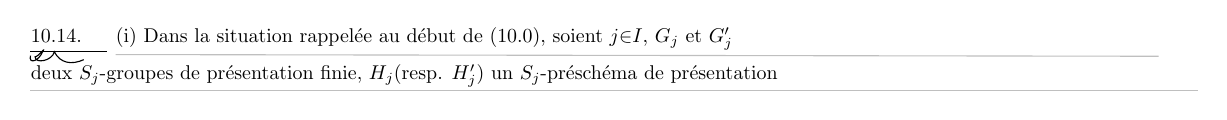
\begin{tikzpicture}[scale=.72,transform shape]
\node[anchor=base west,inner sep=0pt] at (0,0) {10.14.};
\node[anchor=base west,inner sep=0pt] at (1.5,0) {(i) Dans la situation rappelée au début de (10.0), soient $j\handwritten{\in}I$, $G_j$ et $G'_j$};
\node[anchor=base west,inner sep=0pt] at (0,-.65) {deux $S_j$-groupes de présentation finie, $H_j$(resp. $H'_j$) un $S_j$-préschéma de présentation};
\handwritten{\draw (0,-.16)--(1.35,-.16);
\draw (0,-.23) .. controls (-.04,-.38) and (.14,-.34) .. (.22,-.15) .. controls (.27,-.06) and (.14,-.25) .. (.08,-.25) .. controls (.08,-.38) and (.39,-.32) .. (.42,-.16) .. controls (.52,-.36) and (.72,-.40) .. (.94,-.30);
\draw[opacity=.25] (1.5,-.21)--(19.9,-.24);
\draw[opacity=.25] (0,-.85)--(20.6,-.85);}
\end{tikzpicture}}
\scanpage{41}
\mspage{\handwritten{9}}
% archive sheet number: 40
finie à groupe d'opérateurs $G_j$ (resp. $G'_j$). Posons, pour $i\handwritten{\in}I$, $i\handwritten{>}j$, $G_i=G_j\handwritten{\times}_{S_j}S_i$ et $G=G_j\handwritten{\times}_{S_j}S$, et définissons de même $G'_i$, $G'$, $H_i$,$H$, $H'_i$, et $H'$. Notons $\operatorname{Dihom}_{S\text{-gr.}}((G,\handwritten{\unsure{H|H'|\mathbb{H}|\mathbb{H}'}}),(\handwritten{G}',H'))$ l'ensemble des di-morphismes de $S$-groupes et de $S$-préschémas à groupe d'opérateurs du couple $(G,H)$ dans le couple $(G',H')$. Alors l'application canonique de $\underset{i\handwritten{\geqslant}j}{\underset{\handwritten{\longrightarrow}}{\lim}}{\unsure{B|D|\mathbb{D}}\mathrm{ihom}}_{S_i\text{-gr.}}((G_i,H_i),(G'_i,H'_i))$ dans $\operatorname{Dihom}_{S\text{-gr.}}((G,H),(G',H'))$ est bijective.

(ii) Dans la situation rappelée au début de (10.0), soient $G$ un $S$-groupe \deleted{\unsure{fini}} de présentation finie et $H$ un $S$-préschéma de présentation finie à groupe d'opérateurs $G$; il existe alors un indice $j\handwritten{\in}J$, un $S_j$-groupe de présentation finie $G_j$, un $S_j$-préschéma de présentation finie $H_j$ à groupe d'opérateurs $G_j$ et un di-isomorphisme de $S$-groupes et de $S$-préschémas à groupes d'opérateurs de $(G_j\handwritten{\times}_{S_j}S,H_j\handwritten{\times}_{S_j}S)$ sur$(G,H)$

\deleted{Proposition}\inserted{Définition} 10.15.- Etant donné un $S$-foncteur enngroupes $G$ et un $S$-foncteur $H$ à groupe d'opérate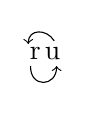
\begin{tikzpicture}[baseline=(r.base)]
\node[anchor=base,inner sep=0pt] (r) at (0,0) {r};
\node[anchor=base,inner sep=0pt] at (.22,0) {u};
\handwritten{\draw[->] (.24,.24) .. controls (.14,.40) and (-.09,.39) .. (-.09,.20);
\draw[->] (-.06,-.08) .. controls (-.07,-.36) and (.27,-.35) .. (.27,-.08);}
\end{tikzpicture}s $G$, on dit que $H$ est un \uline{$S$-foncteur en espaces homogènes sous $G$ pour la topologie $\handwritten{\mathbb{T}}$}, si le morphisme canonique $G\handwritten{\times}_S H\handwritten{\longrightarrow}H\handwritten{\times}_S H$ (défini par $(g,h)\handwritten{\rightsquigarrow}(g.h,h)$ pour $g\handwritten{\in}G(T)$, $h\handwritten{\in}H(T)$) est un épimorphisme de faisceaux pour la topologie $\handwritten{\mathbb{T}}$.

Si $G$ est un $S$-groupe et si $H$ est un $S$-préschéma à \deleted{groupe} groupe d'opérateurs $G$, dire que $H$ est un $S$-préschéma en espaces homogènes sous $G$ pour la topologie $\handwritten{\mathbb{T}}$ revient donc à dire que le morphisme canonique $G\handwritten{\times}_S H\handwritten{\longrightarrow}H\handwritten{\times}_S H$ défini comme précédemment est couvrant pour la topologie $\handwritten{\mathbb{T}}$ (\deleted{Exp.} IV 4.4.3).

De même, dire qu'un $S$-préschéma $H$ à groupe d'opérateurs un $S$-groupe $G$ est un f\deleted{o}\inserted{i}bré principal homogène sous $G$ pour la topologie $\handwritten{\mathbb{T}}$ (\deleted{Exp.} IV 5.1.5) revient à dire (\deleted{Exp.} IV 5.6 (ii)) que le morphisme canonique $G\handwritten{\times}_S H\handwritten{\longrightarrow}H\handwritten{\times}_S H$ est un isomorphisme et que le morphisme structural $H\handwritten{\longrightarrow}S$ est couvrant pour la topologie $\handwritten{\mathbb{T}}$.

\uline{10.16.- Dans la situation rappelée au début de (10.0) , soient $j\handwritten{\in}I$, $G_j$ un $S_j$-grou-}
% The final word continues on the next scan in this package.
\cotefile{10}
\scanpage{42}
\mspage{\handwritten{10}}
\uline{pe de présentation finie, $H_j$ un $S_j$-préschéma de présentation finie à groupe d'\unsure{opératerus|opérateurs} $G_j$. Pour que $\unsure{\mathbb{H}|H}=H_j\handwritten{\times}_{S_j}S$ soit un $S$-préschéma en espaces homogènes sous $\deleted{\unsure{H|G}}$}\margin{\figure{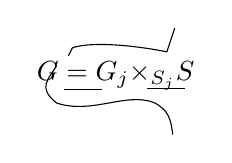
\begin{tikzpicture}[x=.5cm,y=.5cm]\node at (0,0) {$G=G_j\handwritten{\times}_{S_j}S$};\draw (-1.3,-.35) -- (-.35,-.35);\draw (.8,-.32) -- (1.75,-.32);\draw (1.5,1.2) -- (1.3,.6) .. controls (.3,.8) and (-.7,.85) .. (-1.1,.7) -- (-1.2,.5);\draw (-1.5,.25) .. controls (-1.7,-.1) and (-2,-.3) .. (-1.5,-.7) .. controls (-.6,-1) and (.3,-.4) .. (1,-.7) .. controls (1.35,-.9) and (1.4,-1.1) .. (1.45,-1.5);\end{tikzpicture}}}\uline{ (resp. un fibré principal homogène sous $G\inserted{\deleted{\unsure{G=G_j\times_{S_j}S}}}$\unsure{)} pour la }\uuline{topologie fidèlement plate localement de présentation finie}\uline{, il faut et il suffit qu'il existe un indice $i\handwritten{\in}I$, $i\handwritten{\geqslant}j$, tel que $H_i=H_j\handwritten{\times}_{S_j}S_i$ soit un $S_i$-préschéma en espaces homogènes sous $\deleted{\unsure{G_i}}$}\margin{\figure{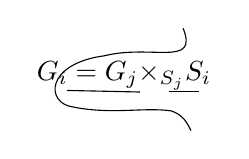
\begin{tikzpicture}[x=.5cm,y=.5cm]\node at (0,0) {$G_i=G_j\handwritten{\times}_{S_j}S_i$};\draw (-1.45,-.38) -- (.4,-.42);\draw (1.15,-.40) -- (1.9,-.40);\draw (1.5,1.2) .. controls (1.9,.2) and (.7,.8) .. (-.5,.5) .. controls (-2,.3) and (-2,-.7) .. (-1.3,-.8) .. controls (-.3,-1) and (.5,-.8) .. (1.2,-.9) .. controls (1.5,-1) and (1.6,-1.2) .. (1.7,-1.4);\end{tikzpicture}}}\uline{ (resp. un fibré principal homogène sous $G_i$).}

Compte tenu de (10.14) et de (EGA IV 8.8.2, 8 8.3 et 8.10.5) , \deleted{\unsure{l'expr|l'exp}} l'énoncé résulte de l\deleted{\unsure{j|f}}\inserted{a} propriété concernant les morphismes \deleted{concernant}\inserted{couvrants} pour la topologie fppf rappelée en (10.0).

\figure{\begin{tikzpicture}[x=.5cm,y=.5cm]
\draw (0,11.6) .. controls (3.4,11.6) and (6.5,11.1) .. (5.1,10.2)
 .. controls (3.7,9.3) and (-1.8,7.2) .. (-.1,7.1)
 .. controls (1.9,7.0) and (4.1,7.6) .. (3.7,5.8)
 .. controls (3.5,4.8) and (2.1,3.8) .. (2.7,2.9)
 .. controls (3.4,1.9) and (5.0,1.1) .. (4.5,0);
\draw (2.45,11.7) .. controls (2.5,7.2) and (2.9,4.0) .. (3.75,.1);
\end{tikzpicture}}
% archive sheet number: 41
\scanpage{43}
\mspage{\handwritten{11}}
\uline{11.- Préschémas en groupes affines.}

\uline{\handwritten{11}.0.}- Notations : soient $S$ un préschéma, $X$ un $S$-préschéma, $f:X\handwritten{\to}S$ le morphisme structural; on pose $\handwritten{\unsure{\mathcal{A}|a}}(X)=f_{\handwritten{*}}(\handwritten{\mathcal{O}}_X)$.

\handwritten{\makebox[0pt][l]{\raisebox{-2ex}{\begin{tikzpicture}[x=1cm,y=1cm]\draw (.05,.14) -- (.05,-.07) -- (.13,-.07);\end{tikzpicture}}}}\uline{Lemme 11.1.- Soient $X$ et $Y$ deux $S$-préschémas quasi-compacts et quasi-séparés sur $S$, $f:X\handwritten{\to}S$ et $g:Y\handwritten{\to}S$ les morphismes structuraux. Alors l'homomorphisme canonique}
\[
\handwritten{\varphi}:\handwritten{\mathcal{A}}(X)\handwritten{\otimes}_{\handwritten{\mathcal{O}}_{\unsure{\mathbb{S}|S}}}\handwritten{\mathcal{A}}(Y)\handwritten{\longrightarrow}\handwritten{\mathcal{A}}(X\handwritten{\times}_S Y)
\]
% Curved pen mark below the tensor-base index.
\figure{\handwritten{\begin{tikzpicture}[x=1cm,y=1cm]\draw (0,.18) .. controls (.25,-.2) and (.8,-.18) .. (1.25,.22);\end{tikzpicture}}}
\margin{\handwritten{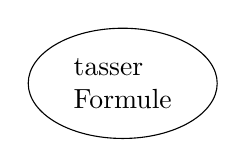
\begin{tikzpicture}[x=1cm,y=1cm]
\draw (0,0) ellipse (1.2 and .7);
\node[align=left] at (0,0) {tasser\\Formule};
\end{tikzpicture}}}
\uline{est un isomorphisme dans chacun des cas suivants :}

\uline{a) $f$ et $g$ sont affines}

\uline{b) $f$ ou $g$ est plat et affine}

\uline{c) $g$ est plat et $f_{\handwritten{*}}(\handwritten{\mathcal{O}}_X)$ est un $\handwritten{\mathcal{O}}_S$-Module plat.}
% Curved pen mark below the star of f in c).
\figure{\handwritten{\begin{tikzpicture}[x=1cm,y=1cm]\draw (0,.15) .. controls (.15,-.16) and (.45,-.16) .. (.6,.16);\end{tikzpicture}}}
\margin{\handwritten{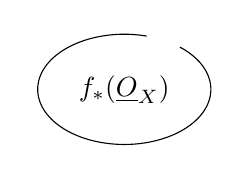
\begin{tikzpicture}[x=1cm,y=1cm]
\draw (.285,.676) arc[start angle=75,end angle=410,x radius=1.1,y radius=.7];
\node at (0,0) {$f_*(\underline{O}_X)$};
\end{tikzpicture}}}

Dans le cas b), on peut supposer que c'est $g$ qui est plat et affine. Posons $S'=\operatorname{Spec}\handwritten{\mathcal{A}}(X)$ $Y'=Y\handwritten{\times}_S\unsure{\mathbb{S}|S}'$, $g'=g\handwritten{\times}_S S'$ et notons $v$ le morphisme $S'\handwritten{\to}S$. Alors $Y$ est quasi-compact et quasi-\linebreak -séparé sur $S$, et, ou bien $S'$est plat sur $S$ (cas c) d'après (EGA III (1.4.15.5)), ou bien $g$ est affine (cas a) et b)). Alors (EGA III 1.4.15 et IV 1.2.7 ou II 1.5.2), on a :
\[
g'_{\handwritten{*}}(\handwritten{\mathcal{O}}_{Y'})=v^{\handwritten{*}}g_{\handwritten{*}}(\handwritten{\mathcal{O}}_Y)=\handwritten{\mathcal{A}}(Y)\handwritten{\otimes}_{\handwritten{\mathcal{O}}_S}\handwritten{\mathcal{O}}_{S'}.
\]

D'après (EGA II 1.2.7), $f$ se \unsure{factorise|favtorise} à travers $v$ au moyen \handwritten{\makebox[0pt][l]{\raisebox{2ex}{\begin{tikzpicture}[x=1cm,y=1cm]\draw (0,0) -- (.17,.09) -- (.43,-.05);\end{tikzpicture}}}}d'un morphisme $p:G\handwritten{\to}S'$, et on a : $X\handwritten{\times}_S Y=X\handwritten{\times}_{S'}Y'$ et $p_{\handwritten{*}}(\handwritten{\mathcal{O}}_X)=\handwritten{\mathcal{O}}_{S'}$. Puisque $v$ et $f$ sont quasi-compacts et quasi-séparés,\deleted{sur} il en est de même de $p$ (EGA IV 1.2.2 et 1.2.4)\handwritten{;} \handwritten{O}u bien $Y$ est plat sur $S$ (cas b) et c)) et alors $Y'$ est plat sur $S'$, ou bien $X$ est affine sur $S$ (cas a)), et alors $p$ est un isomorphisme. Dans le premier cas, on peut de nouveau appliquer (EGA III 1.4.15 et IV 1.2.7), et dans les deux cas, on trouve :
\[
\deleted{\unsure{p_*|q_*}\ \unsure{=}\ \unsure{q'_*|p'_*}}\ p'_{\handwritten{*}}(\handwritten{\mathcal{O}}_{X\handwritten{\times}_S Y})=g'^{\handwritten{*}}p_{\handwritten{*}}(\handwritten{\mathcal{O}}_X)=g'^{\handwritten{*}}(\handwritten{\mathcal{O}}_{S'})=\handwritten{\mathcal{O}}_{Y'}\handwritten{,\ \text{ou }p'=p\times_{S'}Y'.}
\]

D'où :
\[
\handwritten{\mathcal{A}}(X\handwritten{\times}_S Y)=v_{\handwritten{*}}g'_{\handwritten{*}}p'_{\handwritten{*}}(\handwritten{\mathcal{O}}_{X\handwritten{\times}_S Y})=v_{\handwritten{*}}g'_{\handwritten{*}}(\handwritten{\mathcal{O}}_{\handwritten{Y}'})=v_{\handwritten{*}}(\handwritten{\mathcal{A}}(Y)\handwritten{\otimes}_{\handwritten{\mathcal{O}}_S}\handwritten{\mathcal{O}}_{S'})=\handwritten{\mathcal{A}}(Y)\handwritten{\otimes}_{\handwritten{\mathcal{O}}_S}\handwritten{\mathcal{A}}(X)
\]
d'après (EGA II 1.4.7).

\uline{Corollaire 11\handwritten{\unsure{.|/}}2.- On définit un foncteur $X\handwritten{\rightsquigarrow}\operatorname{Spec}\handwritten{\mathcal{A}}(X)$ de la sous-catégorie pleine de $\operatorname{Sch}_{/S}$ des $X$-préschémas plats quasi-compacts et quasi-séparés sur $S$ tels que $\handwritten{\mathcal{A}}(X)$ soit un $\handwritten{\mathcal{O}}_S$-Module plat , dans celle des $S$-préschémas plats et affines sur $S$ . Ce foncteur commute aux produits finis, donc transforme $S$-groupes en $S$-groupes.}
% archive sheet number: 42
\scanpage{44}
\mspage{\handwritten{12}}
\uline{Définition \handwritten{\makebox[0pt][l]{\raisebox{-2ex}{\unsure{\deleted{vu}|vu}}}}11.3.}- Etant donné un $S$-groupe $G$ plat, quasi-compact et quasi-séparé sur $S$, tel que $\handwritten{\unsure{\mathcal{A}|a}}(G)$ soit plat sur $\handwritten{\mathcal{O}}_S$, nous noterons $G_{\mathrm{af}}$ , et nous appellerons \uline{enveloppe affine} de $G$ le $S$-groupe $G_{\mathrm{af}}=\operatorname{Spec}\handwritten{\mathcal{A}}(G)$.


\uline{\handwritten{\makebox[0pt][l]{\raisebox{-2ex}{\unsure{vu}}}}11.4.}- Etant donnés deux $\handwritten{\mathcal{O}}_S$-Modules $\handwritten{\mathcal{E}}$ et $\handwritten{\mathcal{F}}$ quasi-cohérents, notons $\handwritten{\mathcal{H}om}_S(\handwritten{\mathbb{V}}(\handwritten{\mathcal{F}}),\handwritten{\mathbb{V}}(\handwritten{\mathcal{E}}))$ le $S$-foncteur des morphismes de $S$-foncteurs de $\handwritten{\mathbb{V}}(\handwritten{\mathcal{F}})$ dans $\handwritten{\mathbb{V}}(\handwritten{\mathcal{E}})$, et $\handwritten{\mathcal{H}om}_{\handwritten{\mathcal{O}}_S}(\handwritten{\mathbb{V}}(\handwritten{\mathcal{F}}),\handwritten{\mathbb{V}}(\handwritten{\mathcal{E}}))$ le sous-$S$-foncteur de $\handwritten{\mathcal{H}om}_S(\handwritten{\mathbb{V}}(\handwritten{\mathcal{F}}),\handwritten{\mathbb{V}}(\handwritten{\mathcal{E}}))$ formé des $\handwritten{\mathcal{O}}_S$- homomorphismes de $\handwritten{\mathcal{O}}_S$-foncteurs en modules (cf. \deleted{Exp.} I). Alors $\handwritten{\mathcal{H}om}_{\handwritten{\mathcal{O}}_S}(\handwritten{\mathbb{V}}(\handwritten{\mathcal{F}}),\handwritten{\mathbb{V}}(\handwritten{\mathcal{E}}))(T)$ est en correspondance bi\deleted{nu}\inserted{\handwritten{un}}ivoque canonique avec $\deleted{\unsure{\operatorname{Hom}}}\operatorname{Hom}_{\handwritten{\mathcal{O}}_{S\deleted{\unsure{T}}}\text{-}\mathrm{Mod.}}(\handwritten{\mathcal{E}\otimes}_{\handwritten{\mathcal{O}}_S}\handwritten{\mathcal{O}}_T,\deleted{\unsure{(}}\handwritten{\mathcal{F}\otimes}_{\handwritten{\mathcal{O}}_S}\handwritten{\mathcal{O}}_T\deleted{\unsure{)}}$,
\inserted{\handwritten{$\text{i.e.}\quad \mathcal{H}om_{\underline{O}_S}(\mathbb{V}(\mathcal{F}),\mathbb{V}(\mathcal{E}))\simeq\mathcal{H}om_{\underline{O}_S}(\mathbb{W}(\mathcal{E}),\mathbb{W}(\mathcal{F})).$}}


Soit $X$ un $S$-préschéma. Alors l'ensemble des morphismes de $S$-foncteurs de $X$ dans $\handwritten{\mathcal{H}om}_S(\deleted{\handwritten{\unsure{\mathbb{V}|W}}}\handwritten{\mathbb{V}}(\handwritten{\mathcal{F}}),\handwritten{\mathbb{V}}(\handwritten{\mathcal{E}}))$ est en correspondance bi\inserted{\handwritten{un}}nnivoque avec $\operatorname{Hom}_S(X\handwritten{\times}_S\handwritten{\mathbb{V}}(\handwritten{\mathcal{F}}),\handwritten{\mathbb{V}}(\handwritten{\mathcal{E}}))$, donc l'ensemble des morphismes de $S$-foncteurs de $X$ dans $\handwritten{\mathcal{H}om}_{\handwritten{\mathcal{O}}_S}(\handwritten{\mathbb{V}}(\handwritten{\mathcal{F}}),\handwritten{\mathbb{V}}(\handwritten{\mathcal{E}}))$ est en correspondance biunivoque avec un sous-ensemble de $\operatorname{Hom}_S(X\handwritten{\times}_S\handwritten{\mathbb{V}}(\handwritten{\mathcal{F}}),\handwritten{\mathbb{V}}(\handwritten{\mathcal{E}}))=\operatorname{Hom}_{\handwritten{\mathcal{O}}_S\text{-}\mathrm{Mod;}}(\handwritten{\mathcal{E}},\handwritten{\mathcal{A}}(X\handwritten{\times}_S\handwritten{\mathbb{V}}(\handwritten{\mathcal{F}})))$ (EGA II 1.7.13).

\uline{Proposition 11.5.- Soient $X$ un $S$-p\handwritten{\makebox[0pt][l]{\begin{tikzpicture}[x=.2cm,y=.2cm,baseline=-.3ex]\draw (0,-.2) .. controls (.35,0) and (.55,.4) .. (.8,.4);\end{tikzpicture}}}réschéma quasi-compact quasi-séparé sur $S$, $f:X\handwritten{\to}S$ le morphisme structural, $\handwritten{\mathcal{E}}$ et $\handwritten{\mathcal{F}}$ deux $\handwritten{\mathcal{O}}_S$-Modules quasi-cohérents. On suppose vérifiée\deleted{s} l'une des deux conditions suivantes :}

\uline{a) $f$ est affine}

\uline{b) $\handwritten{\mathcal{F}}$ est plat sur $\handwritten{\mathcal{O}}_S$.}

\uline{Alors :}

\margin{\handwritten{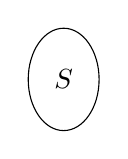
\begin{tikzpicture}\draw (0,0) ellipse (.45 and .65);\node at (0,0) {$S$};\end{tikzpicture}}}
\uline{i) l'homomorphisme canonique $\handwritten{\varphi:\mathcal{A}}(X)\handwritten{\otimes}_{\handwritten{\mathcal{O}}_S}\handwritten{\mathbb{S}}(\handwritten{\mathcal{F}})\handwritten{\longrightarrow\mathcal{A}}(X\handwritten{\times}_S\handwritten{\mathbb{V}}(\handwritten{\mathcal{F}}))$ est un isomorphisme (où $\handwritten{\mathbb{S}}(\handwritten{\mathcal{F}})$ désigne l'Algèbre symétrique de $\handwritten{\mathcal{F}}$).}

\uline{ii) l'ensemble des morphismes de $S$-foncteurs de $X$ dans $\handwritten{\mathcal{H}om}_{\handwritten{\mathcal{O}}_S}(\handwritten{\mathbb{V}}(\handwritten{\mathcal{F}}),\handwritten{\mathbb{V}}(\handwritten{\mathcal{E}}))$ est en correspondance biunivoque avec $\operatorname{Hom}_{\handwritten{\mathcal{O}}_S\text{-}\mathrm{Mod.}}(\handwritten{\mathcal{E}}\ ,\ \handwritten{\mathcal{A}}(X)\handwritten{\otimes\mathcal{F}})$.}

Pour montrer i), d'après (11.1, a) et b)), il suffit de montrer que si $\handwritten{\mathcal{F}}$ est plat sur $\handwritten{\mathcal{O}}_{\unsure{\mathbb{S}|S}}$, \deleted{il en est de même de $\handwritten{\mathbb{S}}(\handwritten{\mathcal{F}})$} alors $\handwritten{\mathbb{V}}(\handwritten{\mathcal{F}})$ est plat sur $S$. D'après (EGA III 1.4.15.5),
% archive sheet number: 43
\scanpage{45}
\mspage{\handwritten{13}}
il suffit de voir que si $\handwritten{\mathcal{F}}$ est plat sur $\handwritten{\mathcal{O}}_S$, \inserted{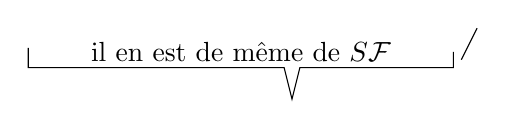
\begin{tikzpicture}[x=1cm,y=1cm,baseline=(n.base)]\node (n) at (0,0) {il en est de même de $\handwritten{\mathbb{S}\mathcal{F}}$};\draw (-2.7,.05)--(-2.7,-.2)--(.55,-.2)--(.65,-.6)--(.75,-.2)--(2.7,-.2)--(2.7,0);\draw (2.8,-.1)--(3,.3);\end{tikzpicture}} ce qui \deleted{résulte des définitions (EGA II 1.7.1), compte tenu d'}\inserted{\handwritten{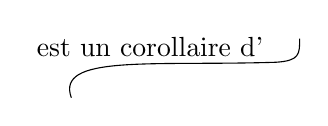
\begin{tikzpicture}[x=1cm,y=1cm,baseline=(n.base)]\node (n) at (0,0) {est un corollaire d'};\draw (-1,-.65) .. controls (-1.2,-.1) and (0,-.25) .. (1.6,-.2) .. controls (1.9,-.18) and (1.9,-.1) .. (1.9,.1);\end{tikzpicture}}}un resultat dû à Daniel LAZARD, suivant lequel tout\deleted{e limite inductive de modules plats est un} module plat\deleted{.} \inserted{\handwritten{sur un anneau est une limite inductive filtrante de modules libres de type fini.}}

\deleted{Remarquons de plus que $\handwritten{\unsure{\mathcal{A}|a}}(X)\handwritten{\otimes}_{\handwritten{\mathcal{O}}_S}\handwritten{\mathbb{S}\mathcal{F}}=\handwritten{\mathbb{S}}(\handwritten{\mathcal{A}}(X)\handwritten{\otimes}_{\handwritten{\mathcal{O}}_S}\handwritten{\mathcal{F}})$ d'après (EGA II 1.1.2), ce qui montre que l'homomorphisme canonique $\handwritten{\mathcal{A}}(X)\handwritten{\otimes}_{\handwritten{\mathcal{O}}_S}\handwritten{\mathcal{F}\longrightarrow}\deleted{\handwritten{\mathbb{S}}}\handwritten{\mathcal{A}}(X)\handwritten{\otimes}_{\handwritten{\mathcal{O}}_S}\handwritten{\mathbb{S}\mathcal{F}}\deleted{\unsure{)}}$ est injectif.}

Montrons maintenant ii). Soit $\handwritten{\alpha}$ un morphisme de $S$-foncteurs de $X$ dans $\handwritten{\mathcal{H}om}_{\handwritten{\mathcal{O}}_S}(\handwritten{\mathbb{V}}(\handwritten{\mathcal{F}}),\handwritten{\mathbb{V}}(\handwritten{\mathcal{E}}))$; il lui correspond un homomorphisme $\handwritten{\rho}$ de $\handwritten{\mathcal{O}}_S$-Modules de $\handwritten{\mathcal{E}}$ dans $\handwritten{\mathcal{A}}(X\handwritten{\times}_S\handwritten{\mathbb{V}}(\handwritten{\mathcal{F}}))=\handwritten{\mathcal{A}}(X)\handwritten{\otimes}_{\handwritten{\mathcal{O}}_S}\handwritten{\mathbb{S}}(\handwritten{\mathcal{F}})$ tel que si $\handwritten{\rho}$ est une $S$-section de $X$, l'homomorphisme
\[
(\handwritten{\mathcal{A}(\eta)\otimes}\operatorname{id}_{\handwritten{\mathbb{S}\mathcal{F}}})\handwritten{\unsure{o|\circ}\rho}:\handwritten{\mathcal{E}\longrightarrow\mathcal{O}}_S\handwritten{\otimes}_{\handwritten{\mathcal{O}}_S}\handwritten{\mathbb{S}\mathcal{F}=\mathbb{S}\mathcal{F}}
\]
corresponde à $\handwritten{\alpha(\eta)}$. Mais puisque $\handwritten{\alpha(\eta)\in}\deleted{\handwritten{\unsure{\mathcal{E}|\mathcal{H}om}}}\handwritten{\mathcal{H}om}_{\handwritten{\mathcal{O}}_S}(\handwritten{\mathbb{V}}(\handwritten{\mathcal{F}}),\handwritten{\mathbb{V}}(\handwritten{\mathcal{E}}))(S)$, $\handwritten{\mathcal{A}(\eta)\otimes}\operatorname{id}_{\handwritten{\mathbb{S}\mathcal{F}}}$ se factorise à travers l'homomorphisme canonique injectif $\handwritten{\mathcal{F}\to\mathbb{S}\mathcal{F}}$. On a donc, pour chaque $S$-section $\handwritten{\eta}$ de $X$\handwritten{,}un diagramme commutatif :
\margin{\handwritten{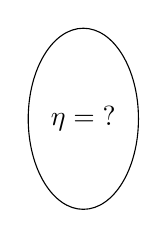
\begin{tikzpicture}
\draw (0,0) ellipse (.7 and 1.15);
\node at (0,0) {$\eta={?}$};
\end{tikzpicture}}}
\diagram{\handwritten{\begin{tikzcd}[ampersand replacement=\&]
\mathcal{E}\arrow[r,"\rho"]\arrow[d]\arrow[d,no head,shift left=1.2pt,shorten >=3pt] \& \mathcal{A}(X)\otimes\mathbb{S}\mathcal{F}\arrow[d]\arrow[dl,"\mathcal{A}(\eta)\otimes\operatorname{id}"']\\
\mathbb{S}\mathcal{F} \& \mathcal{F}\arrow[l]
\end{tikzcd}}}
\handwritten{,}

ce qui montre que $\handwritten{\rho}$ se factorise à travers l'homomorphisme canonique injectif $\handwritten{\mathcal{A}}(X)\handwritten{\otimes}_{\handwritten{\mathcal{O}}_S}\handwritten{\mathcal{F}\longrightarrow\mathcal{A}}(X)\handwritten{\otimes}_{\handwritten{\mathcal{O}}_S}\handwritten{\mathbb{S}\mathcal{F}}$ , donc $\handwritten{\rho}$ peut être considéré comme un homomorphisme de $\handwritten{\mathcal{O}}_S$-Modules de $\handwritten{\mathcal{E}}$ dans $\handwritten{\mathcal{A}}(X)\handwritten{\otimes}_{\handwritten{\mathcal{O}}_S}\handwritten{\mathcal{F}}$ .

Réciproquement, soit $\handwritten{\rho\in}\operatorname{Hom}_{\handwritten{\mathcal{O}}_S\text{-}\mathrm{Mod.}}(\handwritten{\mathcal{E}}\ ,\ \handwritten{\mathcal{A}}(X)\handwritten{\otimes}_{\handwritten{\mathcal{O}}_S}\handwritten{\mathcal{F}})\handwritten{\subset}\operatorname{Hom}_{\handwritten{\mathcal{O}}_S\text{-}\mathrm{Mod}}(\handwritten{\mathcal{E}}\ ,\ \handwritten{\mathcal{A}}(X\handwritten{\times}_S\handwritten{\mathbb{V}}(\handwritten{\mathcal{F}})))$ ; il lui correspond un morphisme $\handwritten{\alpha}$ de $X$ dans $\handwritten{\mathcal{H}om}_{\unsure{\mathbb{S}|S}}(\handwritten{\mathbb{V}}(\handwritten{\mathcal{F}}),\handwritten{\mathbb{V}}(\handwritten{\mathcal{E}}))$ . Pour tout $S$-préschéma $T$ et toute $T$-section $\handwritten{\eta}$ de $X\handwritten{\times}_S T$ , $\handwritten{\alpha(\eta)}$ correspond à $\handwritten{\mathcal{A}(\eta)\otimes}\operatorname{id}_{\handwritten{\mathbb{S}\mathcal{F}\otimes\mathcal{O}}_T}$ , homomorphisme de $\handwritten{\mathcal{E}\otimes}_{\handwritten{\mathcal{O}}_S}\handwritten{\mathcal{O}}_T$ dans $\handwritten{\mathcal{F}\otimes}_{\handwritten{\mathcal{O}}_S}\handwritten{\mathcal{O}}_T$ , donc $\handwritten{d(\eta)\in\mathcal{H}om}_{\handwritten{\mathcal{O}}_S}(\handwritten{\mathbb{V}}(\handwritten{\mathcal{F}}),\handwritten{\mathbb{V}}(\handwritten{\mathcal{E}}))(T)$, ce qui montre que $\handwritten{\alpha}$ est un morphisme de $X$ dans $\handwritten{\mathcal{H}om}_{\handwritten{\mathcal{O}}_S}(\handwritten{\mathbb{V}}(\handwritten{\mathcal{E}}),\handwritten{\mathbb{V}}(\handwritten{\mathcal{F}}))$, ce qui prouve ii).

\deleted{Corollaire 11.6.- Soit $G$ un $S$-groupe plat, quasi-compact et quasi-séparé sur $S$, tel que $\handwritten{\mathcal{A}}(G)$ soit un $\handwritten{\mathcal{O}}_S$-module plat, \deleted{\unsure{et}} $\handwritten{\mathcal{E}}$ un $\handwritten{\mathcal{O}}_S$-Module quasi-cohérent et plat. Alors l'ensemble des applications linéaires}
% archive sheet number: 44
\scanpage{46}
\mspage{\handwritten{14}}
\uline{11.6.}- Soient $G$ un $S$-groupe plat quasi-compact et quasi-séparé sur $S$\handwritten{,} tel que $\handwritten{\unsure{\mathcal{A}|a}}(G)$ soit un $\handwritten{\mathcal{O}}_S$-Module plat $\handwritten{\mathcal{A}}$, et $\handwritten{\mathcal{E}}$ un $\handwritten{\mathcal{O}}_S$-Module quasi-cohérent et plat. \deleted{Nous dirons qu'}\inserted{\handwritten{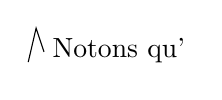
\begin{tikzpicture}[x=1cm,y=1cm,baseline=(n.base)]\node (n) at (0,0) {Notons qu'};\draw (-1.15,-.15)--(-1.05,.28)--(-.95,-.02);\end{tikzpicture}}}un morphisme de $S$-foncteurs de $G$ dans $\inserted{\handwritten{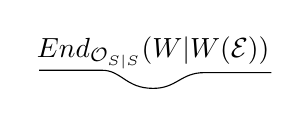
\begin{tikzpicture}[x=1cm,y=1cm,baseline=(n.base)]\node (n) at (0,0) {$\operatorname{End}_{\mathcal{O}_{\unsure{\mathbb{S}|S}}}(\unsure{\mathbb{W}|W}(\mathcal{E}))$};\draw (-1.45,-.22)--(-.65,-.22) .. controls (-.4,-.22) and (-.35,-.45) .. (0,-.45) .. controls (.3,-.45) and (.35,-.25) .. (.65,-.25)--(1.5,-.25);\end{tikzpicture}}}\deleted{\handwritten{\unsure{=|\simeq}\mathcal{H}om_{\mathcal{O}_S}(\mathcal{E},\mathcal{E})}}\handwritten{\simeq\mathcal{H}om}_{\handwritten{\mathcal{O}}_S}(\handwritten{\mathbb{V}}(\handwritten{\mathcal{E}}),\handwritten{\mathbb{V}}(\handwritten{\mathcal{E}}))$ définit une \uline{opéra}-\linebreak\uline{tion} de $G$ sur $\handwritten{\mathcal{E}}$\handwritten{,} si \inserted{\handwritten{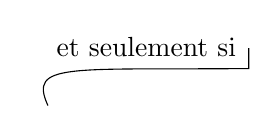
\begin{tikzpicture}[x=1cm,y=1cm,baseline=(n.base)]\node (n) at (0,0) {et seulement si};\draw (-1.25,-.75) .. controls (-1.5,-.2) and (-1,-.3) .. (1.3,-.28)--(1.3,-.02);\end{tikzpicture}}} le morphisme correspondant $\handwritten{\theta}:G\handwritten{\times}_S\handwritten{\mathbb{V}}(\handwritten{\mathcal{E}})\handwritten{\longrightarrow\mathbb{V}}(\handwritten{\mathcal{E}})$ vérifie les deux conditions suivantes :

$1^\circ)$ si $\handwritten{\mu}:G\handwritten{\times}_S G\handwritten{\longrightarrow}G$ désigne le morphisme structural, le diagramme
\diagram{\begin{tikzcd}[ampersand replacement=\&]
G\handwritten{\times}_S G\handwritten{\times}_S\handwritten{\mathbb{V}}(\handwritten{\mathcal{E}})
 \arrow[r,"\operatorname{id}_G\handwritten{\times\theta}"]\arrow[d,"\handwritten{\mu\times}\operatorname{id}_{\handwritten{\mathbb{V}(\mathcal{E})}}"']
\& G\handwritten{\times}_S\handwritten{\mathbb{V}}(\handwritten{\mathcal{E}})\arrow[d,"\handwritten{\theta}"]\\
G\handwritten{\times}_S\deleted{X}\handwritten{\mathbb{V}}(\handwritten{\mathcal{E}})\arrow[r,"\handwritten{\theta}"]
\& \handwritten{\mathbb{V}}(\handwritten{\mathcal{E}})
\end{tikzcd}}
\inserted{\figure{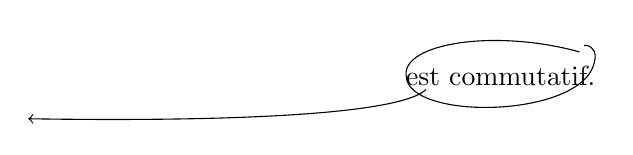
\begin{tikzpicture}[x=1cm,y=1cm]\handwritten{\draw (1,.3) .. controls (-.1,.6) and (-1.25,.4) .. (-1.2,0) .. controls (-1.2,-.6) and (1.2,-.55) .. (1.2,.25) .. controls (1.2,.35) and (1.1,.4) .. (1.06,.38);\draw[->] (-.95,-.18) .. controls (-1.45,-.65) and (-5.8,-.55) .. (-6,-.55);}\node at (0,0) {est commutatif.};\end{tikzpicture}}}

$2^\circ)$ si $\handwritten{\varepsilon}:S\handwritten{\to}G$ est la section unité de $G$, le diagramme
\diagram{\begin{tikzcd}[ampersand replacement=\&]
S\handwritten{\times}_S\handwritten{\mathbb{V}}(\handwritten{\mathcal{E}})
 \arrow[rr,"\handwritten{\varepsilon\times}\operatorname{id}_{\handwritten{\mathbb{V}(\mathcal{E})}}"]
\& \& G\handwritten{\times}_S\handwritten{\mathbb{V}}(\handwritten{\mathcal{E}})\arrow[dl,"\handwritten{\theta}"]\\
\& \handwritten{\mathbb{V}}(\handwritten{\mathcal{E}})\arrow[ul,"\handwritten{\sim}"'] \&
\end{tikzcd}}
\inserted{\figure{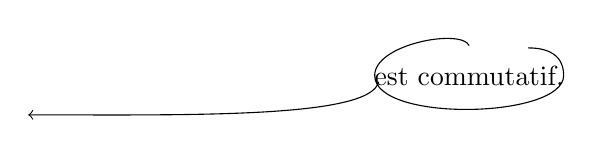
\begin{tikzpicture}[x=1cm,y=1cm]\handwritten{\draw (0,.38) .. controls (-.1,.6) and (-1.2,.4) .. (-1.2,0) .. controls (-1.2,-.6) and (1.2,-.55) .. (1.2,0) .. controls (1.2,.32) and (.9,.35) .. (.75,.35);\draw[->] (-1.15,-.08) .. controls (-1.25,-.55) and (-3.6,-.5) .. (-5.6,-.5);}\node at (0,0) {est commutatif.};\end{tikzpicture}}}

Il revient\inserted{\handwritten{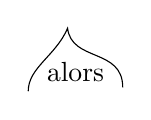
\begin{tikzpicture}[x=1cm,y=1cm,baseline=(n.base)]\node (n) at (0,0) {alors};\draw (-.6,-.25) .. controls (-.6,.05) and (-.25,.2) .. (-.1,.55) .. controls (-.05,.12) and (.6,.3) .. (.6,-.2);\end{tikzpicture}}} au même de dire que le morphisme $\handwritten{\rho}:\inserted{\handwritten{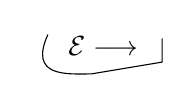
\begin{tikzpicture}[x=1cm,y=1cm,baseline=(n.base)]\node (n) at (0,0) {$\mathcal{E}\longrightarrow$};\draw (-.7,.15) .. controls (-.95,-.4) and (-.45,-.35) .. (-.15,-.35)--(.75,-.2)--(.75,.1);\end{tikzpicture}\begin{tikzpicture}[x=1cm,y=1cm]\draw (0,0)--(0,-.38);\end{tikzpicture}}}\handwritten{\mathcal{A}}(G)\handwritten{\otimes}_{\handwritten{\mathcal{O}}_{\unsure{\mathbb{S}|S}}}\handwritten{\mathcal{E}}$ déduit de $\handwritten{\theta}$ vérifie les deux axiomes suivants :
\margin{\handwritten{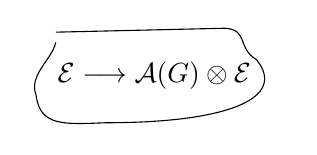
\begin{tikzpicture}
\draw (-1.25,.55)--(.9,.6) .. controls (1.2,.58) and (1.05,.35) .. (1.3,.2) .. controls (1.7,-.3) and (.9,-.6) .. (-.6,-.6) .. controls (-1.15,-.62) and (-1.45,-.65) .. (-1.5,-.25) .. controls (-1.6,0) and (-1.3,.2) .. (-1.25,.42);
\node at (0,0) {$\mathcal{E}\longrightarrow\mathcal{A}(G)\otimes\mathcal{E}$};
\end{tikzpicture}}}

(CM1) Si $\handwritten{\Delta}:\handwritten{\mathcal{A}\longrightarrow\mathcal{A}\otimes\mathcal{A}}=\handwritten{\mathcal{A}}(G\handwritten{\times}_S G)$ est l'homomorphisme $\handwritten{\mathcal{A}(\theta)}$, le diagramme
\diagram{\handwritten{\begin{tikzcd}[ampersand replacement=\&]
\mathcal{A}\otimes\mathcal{A}\otimes\mathcal{A}
\& \mathcal{A}\otimes\mathcal{E}\arrow[l,"\operatorname{id}_{\mathcal{A}}\otimes\rho"']\\
\mathcal{A}\otimes\mathcal{E}\arrow[u,"\Delta\otimes\operatorname{id}_{\mathcal{E}}"]
\& \mathcal{A}\arrow[u,"\rho"']\arrow[l,"\rho"']
\end{tikzcd}}}
\inserted{\figure{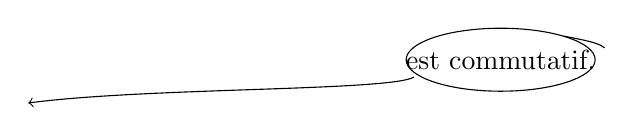
\begin{tikzpicture}[x=1cm,y=1cm]\handwritten{\draw (0,0) ellipse (1.2 and .4);\draw (.8,.3) .. controls (1.05,.25) and (1.24,.22) .. (1.32,.15);\draw[->] (-1.1,-.22) .. controls (-1.4,-.4) and (-4.5,-.35) .. (-6,-.55);}\node at (0,0) {est commutatif.};\end{tikzpicture}}}

(CM2) Si $\handwritten{\eta}:\handwritten{\mathcal{A}\to\mathcal{O}}_S$ est l'homomorphisme $\handwritten{\mathcal{A}(\varepsilon)}$, le diagramme
\diagram{\handwritten{\begin{tikzcd}[ampersand replacement=\&]
\mathcal{O}_S\otimes\mathcal{E}
\& \& \mathcal{A}\otimes\mathcal{E}\arrow[ll,"\eta\otimes\operatorname{id}_{\mathcal{E}}"']\\
\& \mathcal{E}\arrow[ul,"\sim"']\arrow[ur,"\rho"']\&
\end{tikzcd}}}
\inserted{\figure{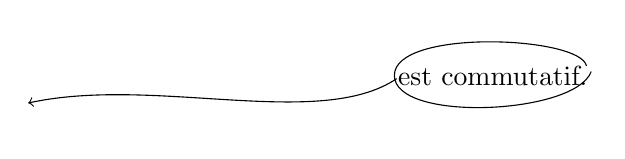
\begin{tikzpicture}[x=1cm,y=1cm]\handwritten{\draw (1.19,.12) .. controls (1.12,.5) and (-1.25,.6) .. (-1.25,0) .. controls (-1.25,-.6) and (1.05,-.5) .. (1.25,.05);\draw[->] (-1.22,-.04) .. controls (-2.2,-.7) and (-4.3,.0) .. (-5.9,-.35);}\node at (0,0) {est commutatif.};\end{tikzpicture}}}

Il revient au même de dire que le morphisme $\handwritten{\theta}_{\mathrm{af}}:G_{\mathrm{af}}\handwritten{\times}_S\handwritten{\mathbb{V}}(\handwritten{\mathcal{E}})\handwritten{\longrightarrow\mathbb{V}}(\handwritten{\mathcal{E}})$ correspondant à $\handwritten{\rho}$ définit une opération de $G_{\mathrm{af}}$ sur $\handwritten{\mathcal{E}}$ \deleted{\handwritten{\unsure{(compar I)|(Exp. I)}}} \inserted{\handwritten{(compar I 4.2)}}.

Par conséquent, il y a correspondance biunivoque entre opérations de $G$ sur $\handwritten{\mathcal{E}}$ et opéra-\linebreak tions de $G_{\mathrm{af}}$ sur $\handwritten{\mathcal{E}}$.

\uline{\handwritten{L}emme} 11.7.- Soient $G$ un $S$-groupe quasi-compact et quasi-séparé sur $S$\handwritten{,}\inserted{\handwritten{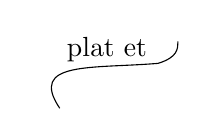
\begin{tikzpicture}[x=1cm,y=1cm,baseline=(n.base)]\node (n) at (0,0) {plat et};\draw (-.6,-.75) .. controls (-1,-.15) and (-.2,-.25) .. (.65,-.18) .. controls (.9,-.1) and (.9,0) .. (.9,.1);\end{tikzpicture}}} tel que $\handwritten{\mathcal{A}}(G)$ soit
% archive sheet number: 45
\scanpage{47}
\mspage{\handwritten{15}}
un $\handwritten{\mathcal{O}}_S$-Module plat $\handwritten{\unsure{\mathcal{A}|a}}$ , et $\handwritten{\mathcal{E}}$ un $\handwritten{\mathcal{O}}_S$-Module quasi-cohérent. On suppose soit que $G$ est affine\inserted{\handwritten{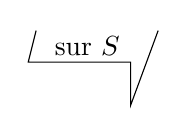
\begin{tikzpicture}[x=1cm,y=1cm,baseline=(n.base)]\node (n) at (0,0) {sur $S$};\draw (-.65,.2)--(-.75,-.2)--(.55,-.2)--(.55,-.75)--(.9,.2);\end{tikzpicture}}}, soit que \deleted{\unsure{G e}}t $\handwritten{\mathcal{E}}$ \deleted{son}\handwritten{soi}t plat\deleted{s} sur $S$. Soit $\handwritten{\rho:\mathcal{E}\to\mathcal{A}\otimes\mathcal{E}}$ un homomorphisme définissant une opé-\linebreak ration de $G$ sur $\handwritten{\mathcal{E}}$. Soit $\handwritten{\mathcal{E}}_{\unsure{o|0}}$ un sous-$\handwritten{\mathcal{O}}_S$-Module quasi-cohérent de $\handwritten{\mathcal{E}}$ tel que l'homomorphisme $\handwritten{\mathcal{E}}_{\unsure{o|0}}\handwritten{\longrightarrow\mathcal{A}\otimes\mathcal{E}}$ déduit de $\handwritten{\rho}$ se factorise à travers l'homomorphisme canonique \handwritten{(}injectif\inserted{\handwritten{, grâce au 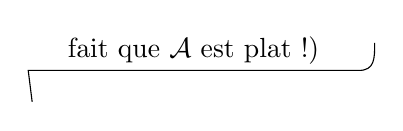
\begin{tikzpicture}[x=1cm,y=1cm,baseline=(n.base)]\node (n) at (0,0) {fait que $\mathcal{A}$ est plat !)};\draw (-2.05,-.65)--(-2.1,-.25)--(2.1,-.25) .. controls (2.3,-.25) and (2.3,-.1) .. (2.3,.1);\end{tikzpicture}}} $\handwritten{\mathcal{A}\otimes\mathcal{E}_{\unsure{o|0}}\longrightarrow\mathcal{A}\otimes\mathcal{E}}$ au moyen de l'homomorphisme $\handwritten{\rho_{\unsure{o|0}}:\mathcal{E}_{\unsure{o|0}}\longrightarrow\mathcal{A}\otimes\mathcal{E}_{\unsure{o|0}}}$. Alors $\handwritten{\rho_{\unsure{o|0}}}$ définit une opération de $G$ sur $\handwritten{\mathcal{E}_{\unsure{o|0}}}$\handwritten{(},\handwritten{(} qu'on appellera \uline{opération induite} sur $\handwritten{\mathcal{E}}_{\unsure{o|0}}$ par $\handwritten{\rho}$, et on dira que $\handwritten{\mathcal{E}}_{\unsure{o|0}}$ est \uline{stable} sous $\handwritten{\rho)}$.

Cela résulte immédiatement des définitions et de (11.\handwritten{6}). On remarquera cependant qu'en général l'application canonique $\handwritten{\mathbb{W}}(\handwritten{\mathcal{E}}_{\unsure{o|0}})\handwritten{\longrightarrow\mathbb{W}}(\handwritten{\mathcal{E}})$ n'est pas injective.

\uline{Lemme 11.8.}- \uline{Soient $G$ un $S$-groupe quasi-séparé et quasi-compact sur $S$ tel que $\handwritten{\mathcal{A}}(G)$ soit un $\handwritten{\mathcal{O}}_{\unsure{\mathbb{S}|S}}$-Module \deleted{\unsure{plat} $\handwritten{\mathcal{A}}$,} libre $\handwritten{\mathcal{A}}$ de base $(\handwritten{\varphi}_i)$, $\handwritten{\mathcal{E}}$ un $\handwritten{\mathcal{O}}_S$-Module quasi-cohérent. On suppose soit que $G$ est affine\inserted{\handwritten{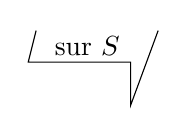
\begin{tikzpicture}[x=1cm,y=1cm,baseline=(n.base)]\node (n) at (0,0) {sur $S$};\draw (-.65,.2)--(-.75,-.2)--(.55,-.2)--(.55,-.75)--(.9,.2);\end{tikzpicture}}}, soit que $G$ et $\handwritten{\mathcal{E}}$ sont plats sur $S$. Soit $\handwritten{\rho:\mathcal{E}\to\mathcal{A}\otimes\mathcal{E}}$ un homomorphisme définis-\linebreak sant une opération de $G$ sur $\handwritten{\mathcal{E}}$, et soit $x\handwritten{\in\Gamma}(S,\handwritten{\mathcal{E}})$. Posons $\handwritten{\rho}(x)=\handwritten{\sum\varphi}_i\handwritten{\otimes x}_i$, où les $x_i\handwritten{\in\Gamma}(S,\handwritten{\mathcal{E}})$ sont bien déterminés par cette relation). Alors le sous-module\inserted{\handwritten{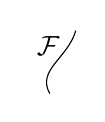
\begin{tikzpicture}[x=1cm,y=1cm,baseline=(n.base)]\node (n) at (0,0) {$\mathcal{F}$};\draw (.35,.2) .. controls (.25,-.15) and (-.15,-.3) .. (.02,-.6);\end{tikzpicture}}} de $\handwritten{\mathcal{E}}$ engendré par les $x_i$ est stable sous $\handwritten{\rho}$,\deleted{et contient $x$.}\inserted{quasi-cohérent} et de type fini sur $\handwritten{\mathcal{O}}_S$, et $x\handwritten{\in\Gamma}(S,\handwritten{\mathcal{F}})$.}
\figure{\handwritten{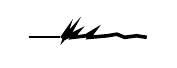
\begin{tikzpicture}[x=1cm,y=1cm]\draw[line width=.7pt] (0,0) -- (.4,0);\draw[line width=1.3pt] (.42,-.01) -- (.49,.09) -- (.46,0) -- (.55,.1) -- (.5,.01) -- (.62,.07) -- (.56,0) -- (.73,.02) -- (.83,.08) -- (.77,0) -- (1,.02) -- (1.12,.04) -- (1.22,0) -- (1.37,.02) -- (1.5,0);\end{tikzpicture}}}

\deleted{Soit $\handwritten{\mathcal{F}}$ le sous-module de $\handwritten{\mathcal{E}}$ engendré par les $x_i$\unsure{,|.}} \handwritten{I}l est clair que $\handwritten{\mathcal{F}}$ est quasi-cohérent et de type fini. L'axiome (CM1) montre que $\handwritten{\sum\Delta}(\handwritten{\varphi}_i)\handwritten{\otimes}x_i=\handwritten{\sum\varphi}_i\handwritten{\otimes\rho}(x_i)$ ; d'autre part, $\handwritten{\Delta(\varphi}_i\handwritten{)=\sum\varphi}_j\handwritten{\otimes}a_{ij}$ , d'où $\handwritten{\sum\varphi}_j\handwritten{\otimes}a_{ij}\handwritten{\otimes}x_i=\handwritten{\sum\varphi}_i\handwritten{\otimes\rho}(x_i)$, d'où, puisque les $\handwritten{\varphi}_i$ forment une base de $\handwritten{\mathcal{A}}$, $\handwritten{\rho}(x_i)=\handwritten{\sum}a_{ji}\handwritten{\otimes}x_{\handwritten{i}}$, où $a_{ji}\handwritten{\in\Gamma}(S,\handwritten{\mathcal{A}})$, ce qui montre que $\handwritten{\rho(\mathcal{F})\subset\mathcal{A}\otimes\mathcal{F}}$, donc $\handwritten{\mathcal{F}}$ est stable sous $\handwritten{\rho}$. Enfin l'axiome (CM2) montre que $x=\handwritten{\sum_i\eta}(\handwritten{\varphi}_i)x_i\handwritten{\in\Gamma}(S,\handwritten{\mathcal{F}})$.

\uline{Proposition 11.9.- Soit $G$ un $S$-groupe quasi-compact quasi-séparé sur $S$ tel que $\handwritten{\mathcal{A}}=\handwritten{\mathcal{A}}(G)$ de-\linebreak vienne localement libre après extension fidèlement plate quasi-compacte de la base $S$ (ce qui} est le cas\inserted{\handwritten{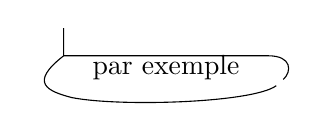
\begin{tikzpicture}[x=1cm,y=1cm,baseline=(n.base)]\node (n) at (0,0) {par exemple};\draw (-1.3,.5)--(-1.3,.15) .. controls (-1.75,-.2) and (-1.5,-.3) .. (-1.2,-.38) .. controls (-.6,-.5) and (1.1,-.45) .. (1.4,-.23);\draw (-1.3,.15)--(1.3,.15) .. controls (1.6,.15) and (1.6,-.05) .. (1.49,-.15);\end{tikzpicture}}} lorsque $G$ est un groupe réductif, comme nous\deleted{\unsure{l}} le verrons dans \deleted{l'exposé} \handwritten{$\overline{\underline{\mathrm{XXV}}}$}), \uline{et} \uline{soit $\handwritten{\mathcal{E}}$ un $\handwritten{\mathcal{O}}_S$-\deleted{module}\handwritten{Module} quasi-cohérent . On suppose soit que $G$ est affine\inserted{\handwritten{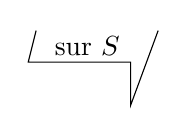
\begin{tikzpicture}[x=1cm,y=1cm,baseline=(n.base)]\node (n) at (0,0) {sur $S$};\draw (-.65,.2)--(-.75,-.2)--(.55,-.2)--(.55,-.75)--(.9,.2);\end{tikzpicture}}}, soit que $G$ et $\handwritten{\mathcal{E}}$ sont plats sur $S$. Soit $\handwritten{\rho:\mathcal{E}\longrightarrow\mathcal{A}\otimes\mathcal{E}}$ un homomorphisme définissant une opération de $G$ sur $\handwritten{\mathcal{E}}$.}
% archive sheet number: 46
\scanpage{48}
\mspage{\handwritten{16}}
\uline{Alors, pour tout sous-$\handwritten{\mathcal{O}}_S$-Module quasi-cohérent $\handwritten{\mathcal{F}}$ de $\handwritten{\mathcal{E}}$ il existe un plus petit sous-$\handwritten{\mathcal{O}}_S$-Mo-\linebreak dule quasi-cohérent $\handwritten{\widetilde{\mathcal{F}}}$ de $\handwritten{\mathcal{E}}$ contenant $\handwritten{\mathcal{F}}$ qui soit stable sous $\handwritten{\rho}$.}\inserted{\figure{\handwritten{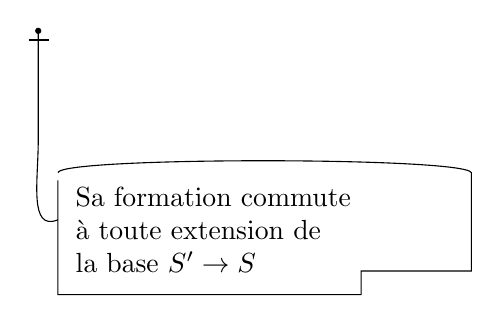
\begin{tikzpicture}[x=1cm,y=1cm]
\draw (.25,.1) .. controls (-.12,-.05) and (0,.6) .. (0,1.1) -- (0,2.5);
\fill (0,2.5) circle (.04);\draw[line width=.8pt] (-.12,2.38) -- (.14,2.38);
\draw (.25,.7) .. controls (.3,.9) and (5.4,.9) .. (5.5,.7) -- (5.5,-.55) -- (4.1,-.55) -- (4.1,-.85) -- (.25,-.85) -- (.25,.60);
\node[align=left,anchor=west] at (.35,-.03) {Sa formation commute\\à toute extension de\\la base $S'\to S$};
\end{tikzpicture}}}}\uline{Lorsque $\handwritten{\mathcal{F}}$ est de type \deleted{\illegible{1}} fini, il en est de même de $\handwritten{\mathcal{F}}$.}

On se ramène aisément\inserted{\handwritten{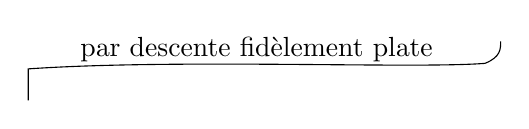
\begin{tikzpicture}[x=1cm,y=1cm,baseline=(n.base)]\node (n) at (0,0) {par descente fidèlement plate};\draw (-2.9,-.65)--(-2.9,-.25) .. controls (-1,-.12) and (2,-.25) .. (2.9,-.18) .. controls (3.1,-.1) and (3.1,0) .. (3.1,.1);\end{tikzpicture}}} au cas où $\handwritten{\unsure{\mathcal{A}|a}}$ est un $\handwritten{\mathcal{O}}_S$-Module libre, auquel cas la proposition est conséquence du lemme 11.8.

\figure{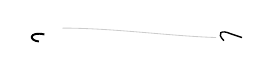
\begin{tikzpicture}[x=1cm,y=1cm]\draw[line width=.7pt] (.12,.04) .. controls (-.08,.08) and (-.08,-.04) .. (.05,-.05);\draw[gray!40,line width=.3pt] (.35,.12) .. controls (1,.12) and (1.7,.02) .. (2.3,0);\draw[line width=.5pt] (2.4,-.04) .. controls (2.3,.06) and (2.37,.1) .. (2.48,.05)--(2.63,0);\end{tikzpicture}}
\uline{Corollaire 11.10.- \deleted{Soit}\inserted{Soient} $S$ un \deleted{pré} schéma \deleted{affine}\inserted{\handwritten{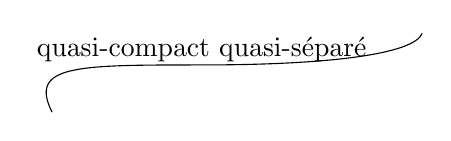
\begin{tikzpicture}[x=1cm,y=1cm,baseline=(n.base)]\node (n) at (0,0) {quasi-compact quasi-séparé};\draw (-1.9,-.8) .. controls (-2.2,-.2) and (-1.6,-.2) .. (0,-.2) .. controls (1.7,-.2) and (2.7,-.05) .. (2.8,.2);\end{tikzpicture}}}, $G$ un $S$-groupe quasi-séparé\inserted{\handwritten{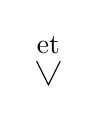
\begin{tikzpicture}[x=1cm,y=1cm,baseline=(n.base)]\node (n) at (0,0) {et};\draw (-.15,-.2)--(0,-.5)--(.15,-.2);\end{tikzpicture}}}quasicompact sur $S$ , tel que $\handwritten{\mathcal{A}}(G)$ devienne \deleted{\unsure{libre}} localement libre après extension fidèlement plate quasi-com-\linebreak pacte de la base,$S$, et soit $\handwritten{\mathcal{E}}$ un $\handwritten{\mathcal{O}}_S$-Module quasi-cohérent. On suppose soit que $G$ est affine sur $S$\deleted{\unsure{.}}\handwritten{,}soit que $G$ et $\handwritten{\mathcal{E}}$ sont plats sur $S$,\inserted{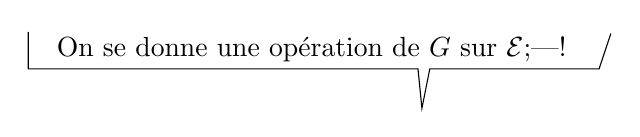
\begin{tikzpicture}[x=1cm,y=1cm,baseline=(n.base)]\node (n) at (0,0) {\uline{On se donne une opération de $G$ sur $\handwritten{\mathcal{E}}$\handwritten{\unsure{;|!}}}};\draw (-3.6,.22)--(-3.6,-.25)--(1.35,-.25)--(1.4,-.75)--(1.5,-.25)--(3.65,-.25)--(3.8,.2);\end{tikzpicture}} \handwritten{A}lors $\handwritten{\mathcal{E}}$ est limite inductive d'une famille fil-\linebreak trante croissante de sous- $\handwritten{\mathcal{O}}_S$-Modules quasi-cohérents de type fini de $\handwritten{\mathcal{E}}$ stables sous} $\handwritten{G}$.

C'est une conséquence immédiate de (11.9) car $\handwritten{\mathcal{E}}$ est \deleted{engendré par ses sections (EGA I 1.4.1\unsure{)} et car l'ensemble des sous-$\handwritten{\mathcal{O}}_S$-Modules quasi-cohérents de type fini de $\handwritten{\mathcal{E}}$ stables sous $G$ est stable par engendrement.}\inserted{\handwritten{limite inductive de ses sous-Modules quasi-cohérents de type fini (EGA I 9.4.9. , $\overline{\underline{\mathrm{IV}}}$ 1.7.7.)}}

\uline{Remarque} 11.10.1. J.P. Serre a remarqué que dans 11.9. (donc aussi dans 11.10) il suffisait de supposer que pour toute ouvert affine $U$ de $S$\unsure{;|,} il existe un morphisme fidè\unsure{l|b}ement plat $U'\handwritten{\to}U$, avec $U'$ affine d'anneau $A'$, tel que $\handwritten{\mathcal{E}\otimes}_U U'$ soit défini par un $A'$-module projectif (pas nécessairement libre). De plus, lorsque $S$ est localement noéthérien régulier et de dimension 1, cette hypothèse peut être remplacée par la seule hypothèse que $G$ soit plat sur $S$ (ce qui implique que $\handwritten{\mathcal{A}}(G)$ est plat); voir à ce sujet \deleted{un exposé de Serre dans SGA\inserted{\handwritten{6}}(1966/67).}\handwritten{1} \inserted{\handwritten{J.P. Serre, \unsure{Sur} le Groupes de Grothendieck des schémas en groupes réductifs déployés, Pub. Math. n° \unsure{39|34}, p. 37-52.}}

\deleted{\uline{Proposition 11.11.- Soient $k$ un corps, $G$ un \deleted{corps} $k$-groupe algébrique. Pour que $G$ soit affine, il faut et il suffit qu'il existe un espace vectoriel de dimension finie $V$, et une immersion fermée de $G$ dans $\underline{\mathrm{GL}}_k(V)$ qui soit un morphisme de $k$-groupes.}}

\deleted{S'il existe un espace vectoriel $V$ de dimension finie et une immersion fermée $u:G\handwritten{\to}\underline{\mathrm{GL}}_k(V)$, puisque $\underline{\mathrm{GL}}_k(V)$ est affine (E\deleted{xp}\inserted{XP}. I, 4.5), il en est de même de $G$ (EGA I 4.2.3).}

\deleted{Réciproquement, supposons $G$ affine. Notons $A$ l'algèbre de $G$. Puisque $G$ opère sur lui-mê-\linebreak me par translations à gauche, il opère aussi sur $A$, cette opération se traduisant par l'appli-\linebreak cation \deleted{\unsure{diagona|diagonal}} diagonale $\handwritten{\Delta}:A\handwritten{\longrightarrow}A\handwritten{\otimes}_k A$. D'après (11.1\handwritten{0}), $A$ (en tant qu'espace vectoriel) est réunion d'une famille filtrante croissante $(V_i)_{i\handwritten{\in}I}$ de sous-espaces vectoriels de dimension fi-\linebreak nie stables sous $G$.}
\deleted{\unsure{Puisque $G$ est de type fini sur $k$, $A$ est de type fini sur $k$, donc il existe} $i_{\unsure{o|0}}\handwritten{\in}I$ tel que $V_{i_{\unsure{o|0}}}$ \unsure{engendre $A$ comme algèbre. L'opération de $G$ sur}}
% archive sheet number: 47
\scanpage{49}
\mspage{\handwritten{17}}
\margin{\handwritten{\figure{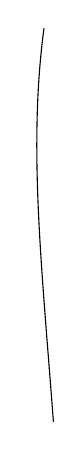
\begin{tikzpicture}\draw (0,0) .. controls (-.20,-1.5) and (-.03,-3) .. (.12,-5);\end{tikzpicture}}}}
\uline{Proposition} 11.\begin{tikzpicture}[x=1cm,y=1cm,baseline=(n.base)]\node (n) at (0,0) {11};\draw (-.15,.3)--(-.02,.3);\draw (-.07,-.08)--(-.07,-.25);\end{tikzpicture}. Soi\deleted{ent}\handwritten{t} \deleted{$k$ un corps}, $G$ un \deleted{schéma en }groupe\deleted{s quasi-compact}\inserted{\handwritten{algébrique sur le}} \deleted{sur}\inserted{\handwritten{corps}} $k$. Les conditions suivantes sont équivalentes:

(i) $G$ est affine.

(ii) $G$ est quasi-affine.

(iii) On peut faire opérer $G$ fidèlement sur un\inserted{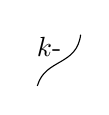
\begin{tikzpicture}[x=1cm,y=1cm,baseline=(n.base)]\node (n) at (0,0) {$k$-};\draw (-.15,-.5) .. controls (-.05,-.15) and (.35,-.25) .. (.4,.15);\end{tikzpicture}}schéma quasi-affine.

(iv) On peut faire opérer $G$ fidèlement sur un vec\deleted{o}\handwritten{t}oriel sur $k$ (pas nécessairement de \deleted{\unsure{t|d}}\inserted{d}imension finie).

(v) \deleted{(si $G$ est de type fini sur $k$),} $G$ est isomorphe à un sous-groupe fermé d'un groupe $\mathrm{Gl}(n)_k$ .

\uline{Démonstration}. On a (i)$\handwritten{\Rightarrow}$(ii) trivialement, et (ii)$\handwritten{\Rightarrow}$(iii), car $G$ opère fidèlement sur lui-même par translations à gauche. On a (iii)$\handwritten{\Rightarrow}$(iv) car si $G$ opère \deleted{fidèlement sur $X$ quasi-affine sur $k$, alors il opère fidèle-\linebreak ment sur l'enveloppe affine $X'=\operatorname{Spec}(\handwritten{\Gamma}($}\inserted{sur $X$ quasi-compact et quasi-séparé sur $k$, il opère aussi} sur le vectoriel $\handwritten{\Gamma}(X,\underline{O}_X)$, grâce au fait que la formation de $f_{\handwritten{*}}(\underline{O}_X)$ ($f:X\handwritten{\to}\operatorname{Spec}k$ le morphisme structural) commute à tout changement de base $S\handwritten{\to}\operatorname{Spec}k$ (EGA IV 1.7.12); donc il opère sur l'enveloppe affine $X'=\operatorname{Spec}(\handwritten{\Gamma}(X,\underline{O}_X))$, et le morphisme canonique $X\handwritten{\to}X'$ est évidemment compatible avec l'action de $G$; ceci dit, si $X$ est quasi-affine i.e. $X\handwritten{\to}X'$ est une immersion ouverte, et si $G$ opère fidèlement sur $X$, il opère fidèlement sur $X'$, ou ce qui revient au même, sur le vectoriel $V=\handwritten{\Gamma}(X,\underline{O}_X)$, ce qui prouve l'implication (iii)$\handwritten{\Rightarrow}$(iv).

\handwritten{S}upposons maintenant \deleted{que $G$ est de type fini, et}\inserted{\handwritten{(iv), i.e.}} que $G$ opère fidèle-\linebreak ment sur le vectoriel $V$. Alors\handwritten{,}en vertu de 11.10\handwritten{,}$V$ est limite inductive de sous-es\handwritten{p}aces vectoriels $V_i$ de di\handwritten{m}ension finie, stables sous l'action de $G$. Si $K_i$ est le noyau de l'action induite de $G$ sur $V_i$ , i.e. de $G\handwritten{\to}\underline{\operatorname{Aut}}_{\inserted{\handwritten{V_i}}}\deleted{\unsure{(V_i)}}$, alors $K_i$ est un sous-schéma fermé de $G$, et l'hypothèse que $G$ opère fidèlement s'exprime aussitôt par le fait que \deleted{$K_{\unsure{1|i|l}}=e$ (grou} l'intersection des $K_i$ est le sous-groupe unité de $G$. Comme $G$ est noethé-%
% archive sheet number: 48
\scanpage{50}%
\mspage{\handwritten{18}}%
rien, il s'ensuit que l'un des $K_i$ est déjà réduit au groupe unité, donc que $G\handwritten{\to}\underline{\operatorname{Aut}}_{\inserted{\handwritten{V_i}}}\deleted{\unsure{(V_i)}}$ est un monomorphisme. C'est donc une immersion fermée en vertu de (1.4.2), ce qui prouve que (iv)$\handwritten{\Rightarrow}$(v). Comme (\deleted{g}v)$\handwritten{\Rightarrow}$(i) triviale-\linebreak ment, cela prouve 11.11\deleted{\unsure{.}} pour $G$ de type fini.

\deleted{Prenons maintenant le cas général, où il reste à prouver que (iv)$\handwritten{\Rightarrow}$(i). Avec les notations de la démonstration précédente, soit $G_i$ le\inserted{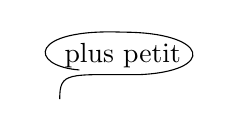
\begin{tikzpicture}[x=1cm,y=1cm,baseline=(n.base)]\node (n) at (0,0) {plus petit};\draw (-.55,-.18) .. controls (-1.2,-.13) and (-1.2,.35) .. (0,.3) .. controls (1.1,.3) and (1.2,-.2) .. (.2,-.24) .. controls (-.7,-.24) and (-.8,-.2) .. (-.8,-.55);\end{tikzpicture}} sous-groupe fermé de $\operatorname{Aut}(V_i)$ par le\handwritten{q}uel\inserted{\begin{tikzpicture}[x=1cm,y=1cm,baseline=(n.base)]\node (n) at (0,0) {peut};\draw (-.45,-.65) .. controls (-.5,-.2) and (-.1,-.3) .. (.4,-.2) .. controls (.5,-.15) and (.5,-.1) .. (.5,-.05);\end{tikzpicture}} se factoriser $G\handwritten{\to}\underline{\operatorname{Aut}}_{\inserted{\handwritten{V_i}}}\deleted{(V_i)}$ \deleted{(existe} (un tel groupe existe, \deleted{puisque} comme intersection de tous ceux par lesquels se factorise $G\handwritten{\to}\deleted{\unsure{\operatorname{Aut}(V_i)}}\inserted{\underline{\operatorname{Aut}}_{V_i}}$). Si $V_j\handwritten{\supset}V_i$, on voit alors tout de suite que $G_j$ invarie $V_i$ , et que le morphisme correspondant $G_j\handwritten{\to}\underline{\operatorname{Aut}}_{V_i}$ se facto-\linebreak rise par $G_i$ . De cette façon, les $G_i$ forment un système projectif de grou-\linebreak pes affines sur $k$, et on a un morphisme naturel $G\handwritten{\longrightarrow}G'=\underset{\handwritten{\longleftarrow}}{\lim}G_i$ , où $G'$ est lui-même un groupe affine (EGA IV 8.2.3). L'hypothèse que $G$ opère \uline{fidèlement} sur $V$ s'exprime alors par\deleted{\unsure{r}} le fait que $G\handwritten{\to}G'$ est un monomor-\linebreak phisme. On a donc trouvé\handwritten{\makebox[0pt][l]{\raisebox{-.5ex}{\begin{tikzpicture}[x=.25cm,y=.25cm]\draw (0,-.5)--(.55,1);\end{tikzpicture}}}}un monomorphisme de $G$ dans un schéma affine, ce qui implique que le schéma quasi-compa\deleted{\unsure{t}}\handwritten{c}t\inserted{\begin{tikzpicture}[x=1cm,y=1cm,baseline=(n.base)]\node (n) at (0,0) {et séparé};\draw (-.6,-.6) .. controls (-.7,-.2) and (-.1,-.2) .. (.6,-.2) .. controls (.8,-.15) and (.8,-.1) .. (.8,-.03);\end{tikzpicture}} $G$ est quasi-affine, i.e. que son faisceau structural est ample, en vertu de EGA IV 18.12.17 . En \handwritten{d}'autres termes, posant $H=\operatorname{Spec}\handwritten{\Gamma}(G,\underline{O}_G)$ , le morphisme canonique $G\handwritten{\to}H$ est une immersion ouverte. Notons maintenant que $H$ est de façon naturelle un schéma en groupes, et $G\handwritten{\to}H$ un homomorphisme de groupes, grâce à 11.2 . Cet homomorphisme est évidemment dominant, il reste à prouver que c'est un isomorphisme, ce qui résulte\deleted{ra d\unsure{e|a}} du lemme suivant:}
\margin{\handwritten{\figure{\begin{tikzpicture}
\draw (.39,.31) .. controls (.5,.55) and (-.25,.5) .. (-.6,.1) .. controls (-1,-.5) and (.25,-.5) .. (.55,-.05) .. controls (.7,.2) and (.5,.3) .. (.34,.28);\node at (0,0) {$\supset$};
\end{tikzpicture}}}}

\deleted{\uline{Lemme} 11.11.1.\handwritten{\unsure{,}} Soient $\deleted{\unsure{G}}\handwritten{H}$ un schéma en groupes sur un corps\inserted{\begin{tikzpicture}[x=1cm,y=1cm,baseline=(n.base)]\node (n) at (0,0) {$k$};\draw (-.35,.08) .. controls (-.2,.08) and (-.15,-.2) .. (0,-.5)--(.3,.1);\end{tikzpicture}}\handwritten{.} \deleted{$G$ un sous-} Alors tout sous-schéma en groupes ouvert\inserted{\begin{tikzpicture}[x=1cm,y=1cm,baseline=(n.base)]\node (n) at (0,0) {$G$};\draw (.3,.18) .. controls (.3,-.15) and (-.2,-.45) .. (-.15,-.65);\end{tikzpicture}} de $H$ est aussi fermé.}
\margin{\handwritten{\figure{\begin{tikzpicture}\draw (0,0)--(.03,-.8);\end{tikzpicture}}}}

\deleted{Il revient au même de dire que l'ensemble $H-G$ est ouvert, i.e. est un voisinage de chacun de ses points\deleted{,} $x$ . Or , toute extension de corps $k'/k$ définissant un morphisme $\operatorname{Spec}k'\handwritten{\to}\operatorname{Spec}k$ qui est universellement}
% archive sheet number: 49
\scanpage{51}
\mspage{\handwritten{19}}
% archive sheet number: 50

\deleted{ouvert (EGA IV 2.4.9), il \deleted{pas} suffit de prouver qu'i\deleted{\unsure{o|h}}\inserted{l} existe une telle extension $k'$ et un point $x'$ de $H'=H\otimes_k k'$ au dessus de $x$, tels que $H'-G'$ soit un voisinage de $x'$. Or \deleted{on}\handwritten{il} suffira de prendre \deleted{$k$} $k'=k(x)$, de sorte que $G'$ admet un point $x'$ rationnel sur $k'$ au dessus de $x$. Alors l'ouvert dans $H'$ translaté de $G'$ par $x'$ contient $x'$ et est contenu dans $H'-G'$\handwritten{,}\deleted{\unsure{qui}} qui est donc un voisinage de $x'$, ce qui achève la démonstration de 11.11.}

\uline{Remarque} 11.11.\deleted{\unsure{3|1}}\handwritten{1}. \deleted{Monsieur} M. Raynaud nous signale qu'on peut générali-\linebreak ser 11.11 au cas d'un schéma en groupes quasi-compact et quasi-s\deleted{p}\handwritten{é}\deleted{\unsure{é|e}}\handwritten{p}aré $G$ sur un schéma\inserted{\begin{tikzpicture}[x=1cm,y=1cm,baseline=(n.base)]\node (n) at (0,0) {$S$ localement n\oe{} thérien};\draw (-2.1,.1) .. controls (-2.2,-.2) and (-1.8,-.2) .. (-.8,-.2)--(-.7,-.65)--(-.65,-.2)--(2.1,-.2)--(2.2,.1);\end{tikzpicture}} régulier de dimension $\handwritten{\leqslant}1$, en supposant de plus $G$ \uline{plat} sur $S$. \begin{tikzpicture}[x=1cm,y=1cm,baseline=(n.base)]\node (n) at (0,0) {On};\node at (.12,-.26) {\handwritten{n}};\draw (-.03,.33)--(.08,.33);\fill (.18,.33) circle (.018);\end{tikzpicture} a alors équivalence des conditions suivantes:

(i) $G$ est affine sur $S$.

(ii) $G$ est quasi-affine sur $S$.

(iii) \unsure{G|O}n peut faire opérer $G$ fidèlement sur un $S$-schéma quasi-affine.

(iv) On peut faire opérer $G$ fidèlement sur un Module quasi-cohérent plat sur $S$.

(v) (Si $G$ est de type fini sur $S$\inserted{\begin{tikzpicture}[x=1cm,y=1cm,baseline=(n.base)]\node (n) at (0,0) {et $S$ noethérien\handwritten{?}};\draw (-1.25,.3) .. controls (-1.9,.2) and (-1.8,-.2) .. (-1.5,-.2)--(-.9,-.25)--(-.9,-.7)--(-.8,-.25)--(1.55,-.25) .. controls (1.9,-.2) and (1.9,.3) .. (1.5,.35)--(1.15,.35);\end{tikzpicture}}) $G$ est isomorphe à un sous-groupe fermé d'un $\text{\uline{Aut}}_V$, où $V$ est un Module localement libre de type fini sur $\handwritten{\unsure{\mathbb{S}|S}}$.

% Handwritten relocation arrow, from the lower remark towards the upper remark.
\margin{\figure{\handwritten{\begin{tikzpicture}[x=0.35cm,y=0.35cm]\draw (1,0) .. controls (0.1,-0.3) and (0.1,0.1) .. (0.1,0.7) -- (0.1,2) .. controls (0.1,2.7) and (0.4,2.8) .. (1,2.8);\draw (0.2,2.5) .. controls (-.6,3.5) and (-.7,6.2) .. (-.9,8.0);\draw[->] (-.92,8.15) .. controls (-.97,9.3) and (-1,10.5) .. (-.8,11) .. controls (-.4,12) and (0.5,12.4) .. (1.6,12.5);\end{tikzpicture}}}}
\deleted{\uline{Remarque} 11.11.2. Avec les notations de la démonstration précédente, on voit facilement (une fois qu'on sait que $G$ est affine) que \unsure{G'|l'}homomor-\linebreak phisme $G\handwritten{\longrightarrow}G'=\underset{\handwritten{\longleftarrow}}{\lim}G_i$ est un isomorphisme, ce qui donne pour $G$ un théorème de structure\handwritten{,} qui sera \deleted{repris}\inserted{prouvé} par une autre méthode dans 11.1\deleted{\unsure{3}}\handwritten{5}.}
\scanpage{52}
\mspage{\handwritten{20}\,\raisebox{.5ex}{\begin{tikzpicture}[x=1cm,y=1cm,baseline=0pt]\draw[line width=.6pt] (0,.04)--(.025,0)--(0,-.025);\end{tikzpicture}}}
% archive sheet number: 51

\deleted{Notons $\handwritten{\varphi}_i:G\handwritten{\longrightarrow}\text{\uline{GL}}_k(V_i)$ le morphisme déterminé par l'opération de $G$ sur $V_i$, et $\handwritten{\varphi}:G\handwritten{\longrightarrow}\text{\uline{GL}}_k(A)$ le morphisme déterminé par l'opération de $G$ sur $A$. Alors, puisque $A$ est réunion des $V_i$, $\operatorname{Ker}\handwritten{\varphi}$ est \unsure{intrésection|intersection} des $\operatorname{Ker}\handwritten{\varphi}_i$; or $\operatorname{Ker}\handwritten{\varphi}$ est le $k$-groupe unité; puisque $G$ est n\oe{} thérien, il existe $i\in I$ tel que $\operatorname{Ker}\handwritten{\varphi}_i$ soit le $k$-groupe unité, ce qui implique (\deleted{\unsure{I}} 1.4.2) que $\handwritten{\varphi}_i$ est une immersion fermée, c.q.f.d.}

\uline{Lemme 11.12.- Soient $k$ un corps, $G$ un $k$-groupe quasi-compact. Posons $A=\handwritten{\unsure{\mathscr{A}|\mathscr{O}}}(G)$. Etant donné $x\in A$, il existe \deleted{un sous-$k$-espace vectoriel de dimension finie}\inserted{une sous-$k$-algèbre de type fini.} $V$ de $A$ tel que $x\in V$, que $\handwritten{\Delta}(V)\subset V\handwritten{\otimes}_k V$ et $u(V)\subset V$, où $u$ désigne l'involution de $A$ correspondant à la symétrie de $G$}

\inserted{D'après (11.3), on peut remplacer $G$ par $G_{\mathrm{af}}$, donc on peut supposer $G$ affine.}

Soit $(\handwritten{\varphi}_i)$ une base de $A$. Alors $\handwritten{\Delta}(x)=\handwritten{\sum\varphi}_i\handwritten{\otimes}a_i$ et $\handwritten{\Delta}(\handwritten{\varphi}_i)=\handwritten{\sum\varphi}_j\handwritten{\otimes}b_{ji}$; l'axiome (HA1) de (\deleted{Exp.} I 4.2) montre que $\handwritten{\sum\varphi}_i\handwritten{\otimes\Delta}(a_i)=\handwritten{\sum\Delta}(\handwritten{\varphi}_i)\handwritten{\otimes}a_i$, d'où $\handwritten{\Delta}(a_i)=\handwritten{\sum}b_{ij}\handwritten{\otimes}a_j$. Soit alors $V$ la \deleted{sous-espace vectoriel}\inserted{sous-$k$-algèbre} de $A$ engendrée par les $b_{ij}$ et les $u(b_{ij})$. Il est clair que $V$ est une $k$-algèbre de type fini. L'axiome (HA1) montre aussi que $\handwritten{\sum\Delta}(\handwritten{\varphi}_j)\handwritten{\otimes}b_{ji}=\handwritten{\sum\varphi}_j\handwritten{\otimes\Delta}(b_{ji})$, et on en déduit que $\handwritten{\Delta}(b_{ij})=\handwritten{\sum}b_{ik}\handwritten{\otimes}b_{kj}$ et que $\handwritten{\Delta}(u(b_{ij}))=\handwritten{\sum}u(b_{kj})\handwritten{\otimes}u(b_{ik})$. Puisque $\handwritten{\Delta}$ est un homomorphisme d'algèbres, on en déduit que $\handwritten{\Delta}(V)\subset V\handwritten{\otimes}_k V$ et $u(V)\subset V$. Enfin l'axiome (HA2) de (\deleted{Exp} I 4.2) montre que $a_i=\handwritten{\sum\eta}(a_j)b_{ij}$ et que $x=\handwritten{\sum\eta}(\handwritten{\varphi}_i)a_i$, si bien que $x\in V$.

\uline{Proposition 11.13.- \deleted{Soit $G$ un $S$-groupe affine} Soient $k$ un corps et $G$ un $k$-groupe affine d'algèbre $A$. . Alors $G$ est limite projective d'un système filtrant croissant de $k$-groupes affines de type fini, dont les morphismes de transition sont fidèlement plats}.

Comme l'ensemble des sous-$k$-algèbres de type fini de $A$ stables par $\handwritten{\Delta}$ et $u$ est stable par engendrement, $A$ est limite inductive d'une famille f ltrante croissante $(B_i)_{i\in I}$ de sous-$k$-algèbres de type fini stables par $\handwritten{\Delta}$ et $u$. Alors, cahque algèbre $B_i$, munie de l'ho-\linebreak momorphisme $B_i\handwritten{\longrightarrow}B_i\handwritten{\otimes}_k B_i$ déduit de $\handwritten{\Delta}$ et de la restriction de $u$ à $B_i$ est munie d'une s\unsure{\deleted{rt}\inserted{tr}|\deleted{tr}\inserted{rt}}ucture d'hyperalgèbre associative augmentée involutive, donc (\deleted{Exp.} I 4.2) est la \begin{tikzpicture}[x=1cm,y=1cm,baseline=(n.base)]\node (n) at (0,0) {$k$};\draw (-.12,.3)--(-.01,.38)--(.03,.4);\end{tikzpicture}-algèbre d'un $k$-groupe affine $G_i$, de type fini sur $k$. Enfin, puisque $A=\underset{\handwritten{\longrightarrow}}{\lim}V_{\begin{tikzpicture}[x=1cm,y=1cm,baseline=(n.base)]\node[inner sep=0pt] (n) at (0,0) {\scriptsize $i$};\draw (.01,-.04)--(.19,-.04)--(.15,-.09);\end{tikzpicture}}$,
% The top of one further character is visible at the clipped lower edge.
$\unsure{G}$
\scanpage{53}
\mspage{\handwritten{21}\,\raisebox{.5ex}{\begin{tikzpicture}[x=1cm,y=1cm,baseline=0pt]\draw[line width=.6pt] (0,-.02)--(.015,.025)--(.04,.04);\end{tikzpicture}}}
% archive sheet number: 52

$G=\underset{\handwritten{\longleftarrow}}{\lim}G_i$ (EGA IV 8.2 3). \deleted{Le fait que} les morphismes de transition sont fidèle-\linebreak \begin{tikzpicture}[x=1cm,y=1cm,baseline=(n.base)]\node (n) at (0,0) {mnet};\draw (-.22,-.16) .. controls (-.26,.43) and (.02,.43) .. (.06,.02) .. controls (.13,-.4) and (.29,-.34) .. (.35,.12);\end{tikzpicture} plats d'après le lemme suivant :
% A handwritten transposition mark joins the n and e of the line-end continuation.


\uline{Lemme \handwritten{11.14}.- Soient $k$ un corps, $G$ et $H$ deux $k$-groupes affines de type fini, $u:G\handwritten{\longrightarrow}H$} un \uline{morphisme de $k$-groupes, et $u^{\unsure{o|0|\circ}}:B\handwritten{\longrightarrow}A$ l'homomorphisme de $k$-algèbres correspondant .} Pour que \uline{$u$ soit fidèlement plat, il faut et il suffit que $u^{\unsure{o|0|\circ}}$ soit injectif.}

la condition est évidemment nécessaire (EGA IV 2.2.3 et $\unsure{0|O}_{\mathrm{IV}}$ 6.6.1). Montrons qu'elle est suffisante. Posons $K=\operatorname{Ker}u$. Alors $G/K$ est un $k$-groupe\inserted{\begin{tikzpicture}[x=1cm,y=1cm,baseline=(n.base)]\node (n) at (0,0) {de type fini};\draw (-1.05,.1)--(-1.05,-.2)--(.05,-.2)--(.11,-.55)--(.18,-.2)--(1.03,-.2);\end{tikzpicture}} (\deleted{Exp.} $\mathrm{VI}_A$ 5.2), et $u$ se factorise en $G\mathrel{\begin{tikzpicture}[x=1cm,y=1cm,baseline=-.5ex]\draw[->] (0,0)--(1,0);\node[inner sep=0pt] at (.5,0) {$\deleted{p}$};\node[inner sep=0pt,above] at (.5,.15) {$\inserted{p}$};\end{tikzpicture}}G/K\overset{v}{\handwritten{\longrightarrow}}H$, où $p$ est fidèlement plat (\deleted{Exp.} $\mathrm{VI}_A$ 3.2) et où $v$ est un monomorphisme de $k$-groupes de type fini, donc une immersion fermée (1.4.2). Puisque $H$ est un schéma affine, et que $v$ est une immersion fermée, $G/K$ est un schéma affine (\unsure{FGA|EGA} I 4.2.3), et, si on note $C$ l'algèbre de $G/K$, l'homomorphisme $v^{\unsure{o|0|\circ}}:B\mathrel{\begin{tikzpicture}[x=1cm,y=1cm,baseline=-.5ex]\draw (0,.08) .. controls (.35,.08) and (.65,.02) .. (1,0);\draw (.74,.14)--(1,0)--(.72,-.14);\draw (.66,.39) .. controls (.71,.26) and (.82,.18) .. (.94,.15);\end{tikzpicture}}C$ est surjectif (loc. cit.) Or, puisque $u^{\unsure{o|0|\circ}}$ est injectif, et que $u^{\unsure{o|0|\circ}}=p^{\unsure{o|0|\circ}}\mathbin{o}v^{\unsure{o|0|\circ}}$, $v^{\unsure{o|0|\circ}}$ est aussi injectif : c'est un isomorphisme, donc $v$ est un isomorphisme, et, puisque $p$ est fidèlement plat, il en est de même de $u$.

\uline{Définitions \handwritten{11.15}}.- Etant donné un corps $k$, un $k$-espace vectoriel $V$, un $k$-groupe $G$ opérant sur $V$, et un vecteur $v\in V$, on dit que $v$ est \uline{semi-invariant} sous $G$ si le sous-espace vectoriel $\handwritten{k.v}$ \deleted{soit}\handwritten{est} stable sous $G$.
\margin{\figure{\handwritten{\begin{tikzpicture}[x=0.45cm,y=0.45cm]\draw (-.16,1.58) .. controls (-.7,1.65) and (-1,1.05) .. (-1,0) .. controls (-1,-1.1) and (-.6,-1.6) .. (0,-1.6) .. controls (.6,-1.6) and (1,-1.05) .. (1,0) .. controls (1,1.05) and (.6,1.6) .. (.03,1.6);\node at (0,0.6) {à la};\node at (0,-0.6) {\unsure{ligne}};\end{tikzpicture}}}}
\figure{\handwritten{\begin{tikzpicture}[x=0.5cm,y=0.3cm]\draw (0,0) -- (2,0) -- (2,1) .. controls (2.5,1.2) and (3.3,1) .. (4,1.1);\end{tikzpicture}}}
Notons $A$ l'algèbre de $G$, et $\handwritten{\rho}:V\handwritten{\longrightarrow}A\handwritten{\otimes}_k V$ l'application linéaire qui dé-\linebreak finit l'opération de $G$ sur $V$. Dire que $v$ est semi-invariant sous $G$ revient à dire \deleted{que, pour} qu'il existe $\handwritten{\lambda}\in A$ tel que, pour tout $w\in kv$, $\handwritten{\rho}(w)=\handwritten{\lambda\otimes}w$. Lorsque $v\handwritten{\neq}0$, l'élément $\handwritten{\lambda\in}A$ est bien déterminé par cette relation, on l'appellera \deleted{\uline{invariant}}\inserted{\handwritten{\uline{poids}}} de l'élément semi-invariant $\handwritten{v}$.

\deleted{D'autre part, $v$ s'interprète comme un élément du bidual de $V$, donc comme une section de $\handwritten{\unsure{\mathbb{V}|V}}(V)$; notons $\handwritten{\varphi}:G\handwritten{\times\mathbb{V}}(V)\handwritten{\longrightarrow\mathbb{V}}(V)$ le morphisme définissant l'opération de $G$ sur $\handwritten{\mathbb{V}}$.} Dire que $v$ est semi-invariant \deleted{revient à dire qu'il existe $\unsure{g\in k|\lambda\in k}$} d'invariant $\handwritten{\lambda}$ revient à dire que $\handwritten{\varphi}(g,v)=\handwritten{\unsure{\lambda|\widetilde{\lambda}|\chi}}(g)v$ pour tout $g\in G(k)$, où $\deleted{\handwritten{\unsure{\varphi:G\longrightarrow\underline{G}_{m,k}|\chi:G\longrightarrow\underline{G}_{m,k}}}}\inserted{\handwritten{\unsure{\lambda|\widetilde{\lambda}|\chi}:G\longrightarrow\underline{G}_{m,k}}}$ est le morphisme défini par $\handwritten{\lambda}$. On voit donc que $\handwritten{\lambda}$ \deleted{correspond à}\inserted{\handwritten{est}} un caractère \deleted{\handwritten{\unsure{$\chi$}}} de $G$, appelé \uline{caractère associé} à l'élément semi-inva-\linebreak riant $v$. \deleted{Enfin nous appellerons poids de l'élément semi-invariant $v$ le poids du caractère $\handwritten{\chi}$ associé à $v$.}
\margin{\handwritten{!}}
\scanpage{54}
\mspage{\handwritten{22}}
% archive sheet number: 53

\uline{Théorème \handwritten{11.16}.}- (Chevalley). So\unsure{e|i}ent $k$ un corps, $G$ un $k$-groupe algébrique affine, $H$ un sous-préschéma en groupes fermé de $G$. Alors il existe un nombre fini d'éléments $a_i$ linéairement indépendants de l'algèbre $A$ de $G$, tels que $H$ soit le plus grand sous-préschéma en groupes fermé de $G$ sous lequel les $a_i$ soient semi-invariants; on peut de plus supposer que tous les $a_i$ ont même \deleted{caractère associé (donc même} poids\deleted{)} sous $H$.

Rappelons que, puisque $G$ est affine, il en est de même de $H$ (\deleted{Exp.} I 4.2.3). Soit $A$ (resp. $B$) l'algèbre de $G$ (resp. $H$); d'après \deleted{\handwritten{§}}EGA I 4.2.3, il existe un idéal $I$ de $A$ tel que $B$ \unsure{qoit|soit} isomorphe à $A/I$\begin{tikzpicture}[x=1cm,y=1cm,baseline=(n.base)]\node[inner sep=0pt] (n) at (0,0) {.};\draw[thin] (-.08,-.07)--(.09,.32);\end{tikzpicture} Puisque $G$ opère sur lui-même par translations à gauche, il opère aussi sur $A$, cette opération se traduisant par l'application diagonale $\handwritten{\Delta}:A\handwritten{\longrightarrow}A\handwritten{\otimes}_k A$ (\deleted{Exp.} I 4.2 et 4.7.2). Puisque $G$ est de type fini sur $k$, $A$ est de type fini sur $k$, donc $I$ \deleted{\unsure{ad}} admet un système fini de générateurs $(g_1,\ldots,g_r)$. Il résulte de (11.9) qu'il existe un sous-espace vectoriel $V$ de dimension finie de $A$ \deleted{sat} stable sous $G$, et contenant chacun des $g_i$.

\margin{\figure{\handwritten{\begin{tikzpicture}[x=0.45cm,y=0.45cm]\draw[rotate=25] (-1,1.3) .. controls (.3,1.65) and (1.8,1.6) .. (1.85,.4) .. controls (1.9,-.6) and (.6,-1.4) .. (-.8,-1.4) .. controls (-1.6,-1.4) and (-2,-1.1) .. (-2,-.7);\node[rotate=25] at (0,0.55) {pas à \unsure{l|la}};\node[rotate=25] at (0,-0.6) {ligne};\end{tikzpicture}}}}
\margin{\figure{\handwritten{\begin{tikzpicture}[x=0.3cm,y=0.3cm]\draw (1,.8) .. controls (.3,1.25) and (-.7,1.1) .. (-.8,.45);\draw (-.8,.25) .. controls (-.4,.05) and (.4,.1) .. (1.15,.3);\end{tikzpicture}}}}
Posons alors $W=V\handwritten{\cap}I$, c'est un espace vectoriel sur $k$ de dimension finie, dont nous noterons $d$ la dimension. Puisque $V$ contient tous les $g_i$, $W$ engendre \deleted{l'algèbre}\inserted{\handwritten{l'ideal}} $I$.

\margin{\figure{\handwritten{\begin{tikzpicture}[x=0.3cm,y=0.3cm]\draw (1,.8) .. controls (.3,1.25) and (-.7,1.1) .. (-.8,.45);\draw (-.8,.25) .. controls (-.4,.05) and (.4,.1) .. (1.15,.3);\end{tikzpicture}}}}
Notons $p:A\handwritten{\longrightarrow}A/I=B$ l'application canonique, et $q=p\handwritten{\otimes}\operatorname{id}_A:A\handwritten{\otimes}_k A\handwritten{\longrightarrow}(A/I)\handwritten{\otimes}_k A$ Alors l'action de $H$ sur $A$ est déterminée par $q\mathbin{o}\handwritten{\Delta}:A\handwritten{\longrightarrow}B\handwritten{\otimes}_k A$. Puisque $H$ est un sous-préschéma en groupes de $G$, l'application diagonale $A/I\handwritten{\longrightarrow}(A/I)\handwritten{\otimes}_k(A/I)=((A/I)\handwritten{\otimes}_k A)/((A/I)\handwritten{\otimes}_k I)$ se déduit de $q\mathbin{o}\handwritten{\Delta}$ par passage au quotient, ce qui montre que $(q\mathbin{o}\handwritten{\Delta})(I)\subset(A/I)\handwritten{\otimes}_k I$, autre-\linebreak ment dit, $I$ est stable sous $H$. Puisque $V$ est stable sous $G$, donc sous $H$, on voit que $W$ est stable sous $H$.

Posons $E=\handwritten{\wedge}^d V$, soit $(w_1,\ldots,w_d)$ une base de $W$ sur $k$, et soit $(e_{\unsure{o|0}},\mathinner{..},e_n)$ une base de $E$ sur $k$ contenant $e_{\unsure{o|0}}=w_1\handwritten{\wedge}\cdots\handwritten{\wedge}w_d$. L'opération de $G$ sur $\handwritten{V}$ détermine canoniquement une opération de $G$ sur $\handwritten{\wedge}^d V$, qui définit une application linéaire $\handwritten{\rho}:E\handwritten{\longrightarrow}A\handwritten{\otimes}_k E$. Posons $\handwritten{\rho}(e_i)=\handwritten{\sum}a_j^i\handwritten{\otimes}e_j$, et $a_i=a_i^{\unsure{o|0}}$. Puisque $W$ est stable sous $H$, si on pose \margin{\figure{\begin{tikzpicture}[x=1cm,y=1cm]\draw[thin] (0,.02)--(.18,-.01);\end{tikzpicture}}}$\handwritten{\sigma}=(p\handwritten{\otimes}\operatorname{id}_E)\mathbin{o}\handwritten{\rho}:E\handwritten{\longrightarrow}(A/I)\handwritten{\otimes}_k E$, il est clair que $\handwritten{\sigma}(e_{\unsure{o|0}})$ est proportionnel à $e_{\unsure{o|0}}$, autrement dit, pour $1\leqq i\leqq n$, on a $a_i\in I$. L'axio\begin{tikzpicture}[x=1cm,y=1cm,baseline=(a.base)]\node[inner sep=0pt] (a) at (0,0) {\unsure{m|n}};\draw (-.12,.05)--(.18,.16);\end{tikzpicture}e (CM1) de (\deleted{Exp.} I 4.7.2) appliqué à
\scanpage{55}
\mspage{\handwritten{23}\,\raisebox{.6ex}{\begin{tikzpicture}[x=1cm,y=1cm,baseline=0pt]\fill (0,0) circle (.018);\end{tikzpicture}}}
% archive sheet number: 54

$\handwritten{\rho}(e_{\unsure{o|0}})=\handwritten{\sum}a_i\handwritten{\otimes}e_i$ montre que $\handwritten{\sum\Delta}(a_i)\handwritten{\otimes}e_i=\handwritten{\sum}a_i\handwritten{\otimes\rho}(e_i)=\handwritten{\sum}a_i\handwritten{\otimes}a_j^i\handwritten{\otimes}e_j$, d'où on dé-\linebreak duit que $\handwritten{\Delta}(a_i)=a_{\unsure{o|0}}\handwritten{\otimes}a_i++\handwritten{\sum_{j\geqslant1}}a_j\handwritten{\otimes}a_i^j$; donc, puisque pour $j\geqslant1$, $a_j\in I$, on voit que $q\mathbin{o}\handwritten{\Delta}(a_i)=p(a_{\unsure{o|0}})\handwritten{\otimes}a_i$, si bien que pou\unsure{r|e} $1\leqq i\leqq n$, $a_i$ est semi-invariant sous $H$ \deleted{d'invara} \deleted{d'invariant}\inserted{\handwritten{de poids}} $p(a_{\unsure{o|0}})$, indépendant de $i$; \deleted{donc tous les $a_i$ sont semi-invariants sous $H$ de même ca-\linebreak ractère associé, donc de même poids. Enfin}\inserted{\handwritten{\begin{tikzpicture}[x=1cm,y=1cm,baseline=(n.base)]\node (n) at (0,0) {Extrayons};\draw (-1.0,-.42) .. controls (-.85,-.2) and (-.5,-.2) .. (0,-.2) .. controls (.7,-.18) and (1,-.18) .. (.9,.08);\end{tikzpicture}}} d\unsure{u|y} système $(a_1,\ldots,a_n)$, \deleted{on peut extraire} un système maximal de vecte\deleted{\unsure{ur}}\handwritten{\unsure{ur}}s linéairement indépendants, dont on peut supposer qu'il se note $(a_{\handwritten{1}},\mathinner{..},a_m)$. \inserted{\handwritten{Alors les $a_i$, $i=1,\mathinner{-\,-},m$ sont lineairement \unsure{indepdants|independants|indépendants}), semi invariants sous $H$, et de même poids.}}

Réciproquement, soit $H'$ un sous-préschéma en groupes fermé de $G$ sous lequel chacun des $a_i$ $(1\leqq i\leqq m)$ est semi-invariant. \inserted{\handwritten{\begin{tikzpicture}[x=1cm,y=1cm,baseline=(n.base)]\node (n) at (0,0) {Montrons que $H'=H$};\draw (-2,-.5) .. controls (-2,-.18) and (-1.8,-.2) .. (-1.4,-.2)--(1.5,-.2) .. controls (1.9,-.2) and (2,-.15) .. (1.95,.08);\end{tikzpicture}}} Il existe de même un idéal $I'$ de $A$ tel que l'algèbre $B'$ de $H'$ soit isomorphe à $A/I'$; notons $p':A\handwritten{\longrightarrow}A/I'$ l'application canonique, et $q'=p'\handwritten{\otimes}\operatorname{id}_A$. Par hypothèse, pour $1\leqq i\leqq m$, il existe $\handwritten{\lambda}_i\in B'$ tel que $q'\mathbin{o}\handwritten{\Delta}(a_i)=\handwritten{\sum}p'(a_j)\handwritten{\otimes}a_i^j=\handwritten{\lambda}_i\handwritten{\otimes}a_i$. Or l'axiome (CM2) de (\deleted{Exp}I 4.7\handwritten{\unsure{;|.}}2) montre que $e_i=\handwritten{\sum\eta}(a_j^i)e_j$, donc que $\handwritten{\eta}(a_j^i)=\handwritten{\delta}_{ij}$ (symbole de Kronecker); l'égalité $\handwritten{\sum}p'(a_j)\handwritten{\otimes\eta}(a_j^i)=\handwritten{\lambda}_i\handwritten{\otimes\eta}(a_i)$ s'écrit donc $p'(a_i)=0$ pour $1\leqq i\leqq m$, car $\handwritten{\eta}(a_i)\handwritten{=\eta}(a_i^{\unsure{o|0}})=0$ pour $1\leqq i\leqq m$; par conséquent, on a $a_i\in I'$ pour $1\leqq i\leqq m$, si bien que $a_i\in I'$ pour $1\leqq i\leqq n$. Donc, si on pose $\handwritten{\sigma}'=(p'\handwritten{\otimes}\operatorname{id}_E)\mathbin{o}\handwritten{\Delta}$, $\handwritten{\sigma}'(e_{\unsure{o|0}})=\handwritten{\sum}p'(a_i)\handwritten{\otimes}e_i$ est proportionnel à $e_{\unsure{o|0}}$, de sorte que $q'\mathbin{o}\handwritten{\Delta}(W)\subset A/I'\handwritten{\otimes}_k W$, autrement dit que $W$ est stable sous $H'$. Puisque $W$ engendre\inserted{\handwritten{\begin{tikzpicture}[x=1cm,y=1cm,baseline=(n.base)]\node (n) at (0,0) {l'ideal};\draw (-.75,-.15) .. controls (-.5,-.1) and (-.2,-.3) .. (-.1,-.5) .. controls (.05,-.1) and (.6,-.35) .. (.75,.02);\end{tikzpicture}}} $I$, $I$ est stable sous $H'$, donc $q'\mathbin{o}\handwritten{\Delta}(I)\subset(A/I')\handwritten{\otimes}_k I$, et $q'\mathbin{o}\handwritten{\Delta}$ définit par passage au quotient une application linéaire $A/I\handwritten{\longrightarrow}(A/I')\handwritten{\otimes}_k(A/I)\handwritten{=((A/I')\otimes_k A)/((A/I')\otimes_k I)}$ donc \deleted{\illegible{14}}\inserted{la restriction à $H'\handwritten{\times_{\begin{tikzpicture}[x=1cm,y=1cm,baseline=(n.base)]\node[inner sep=0pt] (n) at (0,0) {\scriptsize $k$};\draw (-.15,.18)--(-.14,-.12) .. controls (-.12,-.3) and (.14,-.3) .. (.15,-.08)--(.15,.12);\end{tikzpicture}}}H$ du morphisme de multiplication de $G$ se factorise à travers $H$}, ce qui implique que $H'$ est \deleted{in-\linebreak clus dans $H$, \unsure{c.q.f.d.}} un sous-préschéma en groupes de $H$, c.q.f d.

\margin{\handwritten{\unsure{Il doit exister} \unsure{une} \unsure{référence|reference} \unsure{ici} \unsure{Exp.} $\mathrm{VI}_{\unsure{A|a}}$ (\unsure{voir la fin}) \\ \unsure{j'ai|j'écris} \illegible{3} \unsure{en} \illegible{2} \unsure{élémentaire|démonstration}}}
\uline{Théorème} \begin{tikzpicture}[x=1cm,y=1cm,baseline=(n.base)]\node (n) at (0,0) {\handwritten{11.17}};\draw (-.6,-.17)--(.6,-.17);\draw[thin] (-.57,-.11) .. controls (-.55,-.5) and (-.43,-.5) .. (-.42,-.13);\draw (-.42,-.13) .. controls (-.4,-.47) and (-.25,-.47) .. (-.23,-.15) .. controls (-.21,-.51) and (-.04,-.51) .. (.01,-.17) .. controls (.03,-.45) and (.2,-.45) .. (.29,-.17) .. controls (.36,-.29) and (.49,-.29) .. (.53,-.17) .. controls (.64,-.24) and (.69,-.18) .. (.72,-.34);\end{tikzpicture} (Chevalley).- Soient $k$ un corps, $G$ un $k$-groupe affine (non nécessairement al\unsure{-|.}\linebreak gébrique), et $H$ un sous-préschéma en groupes fermé de $G$ \uline{invariant} dans $G$; alors le faisceau quotient (pour la topologie fpqc) $G/H$ est représentable par un $k$-groupe \uline{affine}.

\margin{\figure{\handwritten{\begin{tikzpicture}[x=0.35cm,y=0.35cm]
\draw[thin] (0.45,3.5)--(-.15,3.25);\draw[thin] (0.45,3.5) -- (0.02,3.58) .. controls (-0.35,3.0) and (-0.12,2.4) .. (-0.30,1.95) .. controls (-0.46,1.45) and (-0.01,1.03) .. (-0.17,0.65) .. controls (-0.35,0.30) and (-0.30,0.03) .. (-0.08,0.08);
\draw[thin,->] (0.03,-0.05) .. controls (0.40,-0.05) and (0.52,-0.20) .. (0.38,-0.20);
\end{tikzpicture}}}}
\uline{Premier cas} : \deleted{s}\inserted{\handwritten{S}}upposons d'abord $G$ algébrique. D'après (\deleted{Exp.} $\mathrm{VI}_A$ 3.2), le conoyau $K$ de l'injec-\linebreak tion $H\handwritten{\longrightarrow}G$ existe, \deleted{et} le morphisme canonique $p:G\handwritten{\longrightarrow}K$ est \deleted{fidèlement plat , et quasi-com-\linebreak pact, puisque $G$ est de type fini sur $k$, et que $K$, qui est muni d'une structure de $k$-groupe (Exp. $\mathrm{VI}_A$ 5.2) est séparé sur $k$ (Exp. $\mathrm{VI}_A$ 0.2). Donc $p$ est} couvrant pour la topologie fpqc, \deleted{si bi\deleted{\unsure{u}}en (\deleted{\unsure{Exp.}} IV 4.4.3) que}\inserted{\handwritten{et}} $K$ représente le faisceau quptient $G/H$ pour la topologie fpqc;
\figure{\handwritten{\begin{tikzpicture}[x=.9cm,y=.3cm]\draw[thin] (0,.1) .. controls (.7,-.1) and (1.1,.4) .. (1.5,.05) .. controls (1.8,-.5) and (2.3,-.3) .. (2.5,.1) .. controls (3.7,-.1) and (4.2,.15) .. (5,.05) .. controls (7,.15) and (8,-.15) .. (9,.05) .. controls (11,.12) and (12,-.2) .. (14,0);\end{tikzpicture}}}
\scanpage{56}
% archive sheet number: 55

\handwritten{Supposons. d'abord $k$ algébriquement clos, $G$ réduit et connexe et $H$ réduit. D'après (\uline{BIBLE} \deleted{\unsure{VII|VIII}}\inserted{\deleted{Exp} 4, cor du th.\uline{1}\begin{tikzpicture}[x=1cm,y=1cm,baseline=-.1cm]\draw[thin] (0,-.1).. controls (-.1,-.35) and (-1.5,-.1)..(-1.7,-.4)--(-1.75,-.6)--(-1.8,-.35);\end{tikzpicture}}), il existe une representation lineaire de dimension finie $\rho:G\longrightarrow\mathrm{GL}(V)$ telle que $(\operatorname{Ker}\rho)_{\mathrm{red}}=H$. Par 11.11, $G/\operatorname{Ker}\rho$ est affine. donc $(G/H)/(\operatorname{Ker}\rho/H)$ est affine, donc aussi $G/H$, le groupe $\operatorname{Ker}\rho/H$ étant fini.}

\handwritten{Si $k$ est algébriquement clos, et $G$ et $H$ réduits, alors $(G/H)/(G^{\unsure{\circ|0|o}}/H\cap G^{\unsure{\circ|0|o}})$ est fini,\inserted{ comme quotient de $G/G^{\unsure{\circ|0|o}}$, et\begin{tikzpicture}[x=1cm,y=1cm,baseline=-.1cm]\draw[thin] (0,.05).. controls (0,-.25) and (-1.9,-.15)..(-2,-.35)--(-2.02,-.55);\end{tikzpicture}} $G^{\unsure{\circ|0|o}}/H\cap G^{\unsure{\circ|0|o}}$ est affine, donc $G/H$ est affine.}
\margin{\figure{\handwritten{\begin{tikzpicture}[x=0.2cm,y=0.4cm]\draw (0,8) .. controls (1.2,6.8) and (1,3) .. (1.2,0);\draw (0.8,6.8).. controls (0.7,6.5) and (0.3,6.5)..(-0.2,6.45);\end{tikzpicture}}}}

\figure{\handwritten{\begin{tikzpicture}\draw (0,0) .. controls (3,0.2) and (8,0.2) .. (12,0);\end{tikzpicture}}}
\deleted{\handwritten{\uline{N.B.}1) le th \unsure{entraîne|entraine} que si $G$ est affine algébrique et $H$ invariant, il existe une rep lin\unsure{e|é}aire de dim finie $\rho:G\longrightarrow\mathrm{GL}(V)$ telle que $H=\operatorname{Ker}\rho$}}

\deleted{\handwritten{2) La réf à BIBLE est un corollaire de 11.16, la d\unsure{e|é}monstration est facile mais un peu longue.}}

\deleted{\handwritten{3) Dan la réf à BIBLE Supposer $G$ connexe, car la dém. de BIBLE est \unsure{formulée} dans le cas general\begin{tikzpicture}[x=1cm,y=1cm,baseline=-.1cm]\draw[thin] (0,0).. controls (.45,.12) and (.85,.6)..(1.22,.5).. controls (1.43,.47) and (1.48,.25)..(1.4,.16);\end{tikzpicture}}}
\figure{\handwritten{\begin{tikzpicture}\draw (0,0) .. controls (4,0.4) and (8,0.5) .. (12,0.6);\end{tikzpicture}}}
\scanpage{57}
\mspage{\handwritten{24.}}
% archive sheet number: 56

il s'agit donc de montrer que $K$ est affine.

\deleted{Le théorème est connu dans le cas où $k$ est algébriquement clos\unsure{,} et où $G$ et $H$ sont réduits (Chevalley}\deleted{\unsure{)}}\inserted{\deleted{\handwritten{Supposons d'abord.}}}
\margin{\figure{\handwritten{\begin{tikzpicture}[x=0.4cm,y=0.4cm]\draw (0,0) ellipse (3.1 and 0.9);\node at (0,0) {VOIR CI CONTRE};\draw (-3,0) .. controls (-5,-1) and (-7,-0.4) .. (-8,-0.4);\draw[->] (-8,-0.35)--(-6.9,-0.5);\draw[gray,thin] (-7.6,.45).. controls (-8,-.1) and (-7.3,-.1)..(-7.65,-.35);\end{tikzpicture}}}}

Dans le cas où $k$ est algébriquement clos, et $G$ et $H$ quelconques,\deleted{(\unsure{$(G/H)_{\mathrm{red}}$} est isomorphe à \unsure{$G_{\mathrm{red}}/H_{\mathrm{red}}$} réduit (\unsure{9.2 vi|9.2 iv})}, $(G\handwritten{\times}_k H)_{\mathrm{red}}$ est isomorphe à $(G_{\mathrm{red}})\handwritten{\times}_k(H_{\mathrm{red}})$, donc $(G_{\mathrm{red}})/(H_{\mathrm{red}})$ est isomorphe à $(G/H)_{\mathrm{red}}$. Puisque $(G_{\mathrm{red}})/H_{\mathrm{red}}$ est affine, il en est de même de $G/H$ (EGA I 5.1.10), car, puisque $G/H$ est de type fini sur $k$, son nilradical est nilpotent.

Dans le cas où $k$ est quelconque, $G\handwritten{\otimes}_k\handwritten{\bar{k}}/H\handwritten{\unsure{\oslash|\otimes}}_k\handwritten{\bar{k}}$ est isomorphe à $(G/H)\handwritten{\otimes}_k\handwritten{\bar{k}}$ (9.2 v)), donc puisque le premier est affine, il en est de même du second, donc $G/H$ est affine\handwritten{(ref.)\unsure{'|,}}
\margin{\handwritten{(\qquad)}}

\uline{Deuxième cas} : \handwritten{C}as général . D'après (11.13), l'algèbre $A$ de $G$ est limite inductive d'une famille filtrante croissante $(A_i)_{i\in I}$ de sous-algèbres de type fini de $A$ stables par l'application diagonale et l'involution. D'après (\deleted{Exp.}\inserted{EGA} I 4.2.3), $H$ est affine, et si on note $B$ l'algèbre de $H$, l'homomorphisme $A\handwritten{\longrightarrow}B$ déduit de l'injection $H\handwritten{\longrightarrow}G$ est surjectif. Posons $I=\operatorname{Ker}(A\handwritten{\to}B)$, $I_i=I\handwritten{\cap}A_i$ et $B_i=A_i/I_i$; puisque la structure d'hyperalgèbre associative augmentée involutive de $A$ passe au quotient à travers $I$, on vérifie aisément que celle de $A_i$ passe au quotient à travers $I_i$, si bien que $B_i$ est l'algèbre d'un $k$-groupe affine de type fini $H_i$; il est clair que $B=\lim B_i$. D'après (EGA I 4.2.3), $H_i$ est isomorphe à un sous-préschéma en g\inserted{\handwritten{r\begin{tikzpicture}[x=1cm,y=1cm,baseline=-.1cm]\draw[thin] (-.25,.05)--(-.18,-.3).. controls (-.03,-.12) and (.17,-.17)..(.25,-.1);\end{tikzpicture}}}oupes fermé de $G_i$. D'après (6.7) le fait que $H$ soit invariant dans $G$ s'exprime en disant qu'un certain morphisme $H\handwritten{\times}_k G\handwritten{\longrightarrow}G$ se factorise à travers l'injection $H\handwritten{\longrightarrow}G$, autrement dit que l'homomorphisme correspondant $A\handwritten{\longrightarrow}B\handwritten{\otimes}_k A$ se factorise à travers l'homomorphisme canonique $A\handwritten{\longrightarrow}B$; on vérifie aisément que l'homomorphisme $A_i\handwritten{\longrightarrow}B_i\handwritten{\otimes}_k A_i$ défini de manière analogue se factorise à travers $A_i\handwritten{\longrightarrow}B_i$, donc que $H_i$ est invariant dans $G_i$. D'après ce qui a été vu précédemment, $G_i$ étant de type fini sur\inserted{\handwritten{\ \begin{tikzpicture}[x=1cm,y=1cm,baseline=0cm]\draw[thin] (0,.3)--(-.03,-.35);\end{tikzpicture}}}$k$, $G_i/H_i$ est représentable par un $k$-groupe affine $K_i$, dont nous noterons $C_i$ l'algèbre. Posons alo\deleted{r}\handwritten{\unsure{r|4}}s $C=\underset{\handwritten{\longrightarrow}}{\lim}C_i$, et soit $K=\underset{\handwritten{\longleftarrow}}{\lim}K_i$ le $k$-préschéma affine d'algèbre $K$ (EGA IV 8.2.3).

\margin{\figure{\begin{tikzpicture}[x=1cm,y=1cm]\draw[gray,thin] (0,0).. controls (-.04,1.5) and (-.2,2.7)..(-.03,4.4);\end{tikzpicture}}}

Montrons que $K$ représente $G/H$; pour cela, il suffit de vérifier que \deleted{le diagramme}
\margin{\handwritten{est ce défini ?}}
\diagram{\begin{tikzcd}[ampersand replacement=\&,execute at end picture={\draw[thin] (current bounding box.center) ellipse [x radius=4.2cm,y radius=0.55cm];}]
H\handwritten{\times}_k G \arrow[r,"\handwritten{\sim}"] \& G\deleted{\unsure{\longrightarrow K}}\handwritten{\times_K G}\quad\text{\deleted{est cartésien}}
\end{tikzcd}}
\handwritten{,} et que le morphisme $G\handwritten{\longrightarrow}K$ est couvrant pour la topologie fpqc. (\deleted{\unsure{Exp.}} IV 4.4.3). Or, \deleted{chacun des diagrammes}\inserted{\handwritten{pour chaque $i$, on \unsure{-|a}}}
\diagram{\begin{tikzcd}[ampersand replacement=\&]
H_i\handwritten{\times}_k G_i \arrow[r,"\handwritten{\sim}"] \& G_i\deleted{\unsure{\longrightarrow K_i}}\handwritten{\times_{K_i}G_i}
\end{tikzcd}}
\handwritten{,}\deleted{étant cartésien,}\inserted{\handwritten{donc}} il en est de même d\deleted{\unsure{u|e}}\handwritten{u} \deleted{diagramme}\inserted{\handwritten{morphisme\begin{tikzpicture}[x=1cm,y=1cm,baseline=-.1cm]\draw[thin] (0,.06).. controls (.18,-.15) and (-.85,-.1)..(-.9,-.3)--(-.85,-.47);\end{tikzpicture}}} obtenu en passant à la limite projective; enfin chacun des morphismes
\scanpage{58}
\mspage{\handwritten{25}}
% archive sheet number: 57

$G_i\handwritten{\longrightarrow}K_i$ est fidèlement plat (9.2 (xi)), autrement dit $C_i$ est fidèlement plat sur $A_i$; puisque $A=\underset{\handwritten{\longrightarrow}}{\lim}A_i$ et $C=\underset{\handwritten{\longrightarrow}}{\lim}C_i$, on en déduit que $C$ est fidèlement plat sur $A$\handwritten{,}\deleted{(cf. \unsure{Bour}baki Alg. Comm. \illegible{3}\unsure{)}} si bien que $G\handwritten{\longrightarrow}K$ est un morphisme fidèlement plat. Puisque ce morphisme est affine, il est quasi-compact, donc couvrant pour la topologie fpqc,c.q.f.d.

\deleted{\uline{Corollaire} 11.18. Soient $k$ un corps, $G=D(M)$ un groupe diagonalis\unsure{a}ble sur $k$ (I 4.4), \deleted{$H$ un sous-groupe de} avec $M$ un $\text{\uline{Z}}$-module de type fini, $H$ un sous-groupe algébrique de $G$. Alors $H$ est également diagonalisable.}
\scanpage{60}
% block: heading
\uline{Catégorie tannakienne} (sur un corps $k$) \uline{de} \deleted{grou} \uline{lien un groupe diagonalisable} $G=D(\handwritten{\unsure{\Gamma|T}})$ \handwritten{$(\Leftrightarrow\mathcal{M}$} semi-simple, et pour tout objet simple (ou isotypique) $S$ de $\handwritten{\mathcal{M}}$, de rang $d(S)$, $\operatorname{End}(S)$ est de rang $d(S)^{\handwritten{2}}\handwritten{)}$.

% block: classification and first display
Soit $\deleted{M}\handwritten{\mathcal{M}}$ cette c atégorie. Elle est définie à équivalence près (respectant structures et contraintes) par un élément\inserted{\handwritten{$\xi$\begin{tikzpicture}[x=1cm,y=1cm,baseline=0cm]\draw[thin] (-.1,-.4)--(.18,.3);\end{tikzpicture}}} de $H^{\handwritten{2}}(k,G)$. On a d'autre part
\[
H^{\handwritten{2}}(k,G)\handwritten{\simeq}\operatorname{Hom}(\handwritten{\Gamma},\operatorname{Br}(k))\ ,
\]
donc $\handwritten{\mathcal{M}}$ est définie essentiellement par l'homomorphisme \deleted{cano}
\[
\handwritten{\deleted{\unsure{\xi}}u:\ \Gamma\longrightarrow}\operatorname{Br}(k)\ .
\]

% block: grading and characterization
\deleted{Pour tout} La catégorie $\handwritten{\mathcal{M}}$ est graduée de type $\handwritten{\Gamma}$, les objets homogènes de type $\handwritten{\Gamma}$ sont\inserted{\handwritten{les objets\begin{tikzpicture}[x=1cm,y=1cm,baseline=-.1cm]\draw[thin] (0,.06).. controls (.15,-.18) and (-1.1,-.08)..(-1.25,-.3)--(-1.3,-.5);\end{tikzpicture}}} isotypiques, donc pour tout $i\handwritten{\in\Gamma}$, il y a exactement un objet simple, à isomorphisme près, $\unsure{\mathbb{E}|E}_i$, \deleted{de} homogène de degré $i$. (Il semble que ce soit une deuxième caractérisation des catégories tannakiennes de lien $D(\handwritten{\Gamma})$;\inserted{\handwritten{$\Leftrightarrow$ le pr. \unsure{direct|droit|tensl|tensoriel} de deux isotypiques est isotypique\begin{tikzpicture}[x=1cm,y=1cm,baseline=-.1cm]\draw[thin] (0,.06).. controls (.15,-.18) and (-1.1,-.08)..(-1.25,-.3)--(-1.3,-.5);\end{tikzpicture}}}) Le degré de cet élément est égal à l'ordre\inserted{$d(i)$\begin{tikzpicture}[x=1cm,y=1cm,baseline=-.1cm]\draw[thin] (0,.06).. controls (.15,-.18) and (-1.1,-.08)..(-1.25,-.3)--(-1.3,-.5);\end{tikzpicture}} de $u(i)$ dans $\operatorname{Br}(k)$. Donc l'anneau $K(\handwritten{\mathcal{M}})$ est donné par
\[
\begin{aligned}
K(\handwritten{\mathcal{M}})\handwritten{\subset}\underline{Z}\deleted{(}\handwritten{[}\handwritten{\Gamma}\handwritten{]}\ ,\\
\handwritten{\sum}n_i e^i\handwritten{\in}K(\handwritten{\mathcal{M}})\quad\handwritten{\Longleftrightarrow}\quad n_i\handwritten{\equiv}0\ (d(i))\quad\text{pour tout }i\handwritten{\in\Gamma}
\end{aligned}
\]
La base canonique de $K(\handwritten{\mathcal{M}})$ formée par les objets simples étant formée des $d(i)e^i$. Si $M_i$ est l'objet simple de \deleted{poids} degré $i$, alors $\operatorname{End}(M_i)$ est le corps gauche \deleted{de sur} de centre $k$ dont l'invariant daas $\operatorname{Br}(k)$ est $u(i)$.

% block: cancelled paragraph
\deleted{En termes d'un système de générateurs $({}_i)_{i\,\unsure{I|\in I}}$ de $I$, \deleted{et}(d'un système d'objets \deleted{simples}\inserted{isotypiques} \deleted{$\unsure{M|\mathbb{M}}_i$} \deleted{de type} degré $i$)et des}

\figure{\begin{tikzpicture}[x=1cm,y=1cm]\draw[thin,gray] (0,0)--(0,.4)--(1,.4)--(1,.8)--(12,.8).. controls (12.25,.8) and (12.25,.25)..(12,.25)--(10,.25)--(10,-.1)--(0,-.1)--cycle;\draw (1.15,.65).. controls (1.7,-.6) and (2.1,.8)..(2.7,.1).. controls (3.4,-.3) and (4.5,.7)..(4.8,.5).. controls (5.2,-.1) and (5.9,.2)..(6.3,.3).. controls (6.7,.4) and (6.5,-.1)..(7.1,.05).. controls (7.5,.2) and (7.2,-.1)..(7.9,0).. controls (8.8,-.2) and (9.2,.7)..(10,.55).. controls (10.5,.25) and (10.8,.55)..(11.2,.5);\end{tikzpicture}}

% block: free group case
Si $\Gamma=Z^{(I)}$,\inserted{i.e. $G=G_m^I$,\begin{tikzpicture}[x=1cm,y=1cm,baseline=-.1cm]\draw[thin] (0,.06).. controls (.15,-.18) and (-1.1,-.08)..(-1.25,-.3)--(-1.3,-.5);\end{tikzpicture}} la donnée de $u$\inserted{i.e. de $\handwritten{\xi}$\begin{tikzpicture}[x=1cm,y=1cm,baseline=-.1cm]\draw[thin] (0,.06).. controls (.15,-.18) and (-1.1,-.08)..(-1.25,-.3)--(-1.3,-.5);\end{tikzpicture}} revient à la donnée d'éléments $\handwritten{\xi}_i\handwritten{\in}\operatorname{Br}(k)$. Choisissant pour tout $i$ un objet isotypique non nul de degré $i$, soit $E_i$, et désignant par $A_i=\operatorname{End}(\deleted{\unsure{A|M}}\handwritten{M}_i)$ l'algèbre d'Azymaya associée,\inserted{de classe $\handwritten{\xi}_i$,\begin{tikzpicture}[x=1cm,y=1cm,baseline=-.1cm]\draw[thin] (0,.06).. controls (.15,-.18) and (-1.1,-.08)..(-1.25,-.3)--(-1.3,-.5);\end{tikzpicture}} on réconstitue (à équivalence unique près\deleted{)} respectant tout)
% archive sheet number: 59
\scanpage{61}
% block: reconstruction continued
$\handwritten{\mathcal{M}}$ en termes de la \unsure{famille|faamille} des $A_i$ \deleted{et des entiers $d_i=\operatorname{rang}E_i$} comme suit\deleted{e}. On considère d'abord la catégories sous-additive \deleted{engendrée} ayant comme objets les éléments $\handwritten{\underline{\unsure{Y|\gamma}}}$ de $\underline{N}^{(I)}$, ($\handwritten{\underline{\gamma}}=(\handwritten{\gamma}_i)_{i\handwritten{\in}I}$ étant interprété comme $\handwritten{\bigotimes}E_i^{\handwritten{\gamma}_i}$), \deleted{ou} avec $\operatorname{Hom}(\handwritten{\underline{\gamma}},\handwritten{\underline{\gamma}'})=0$ si $\handwritten{\underline{\gamma}\ne\underline{\gamma}'}$ et $=\bigotimes_{\handwritten{i}} A_i^{\otimes\handwritten{\gamma_i}}$ si $\handwritten{\underline{\gamma}=\underline{\gamma}'}$, la composition des morphismes évidentes. On définit de façon évidente le foncteur $\otimes$ (addition de $\underline{N}^{(I)}$ sur les objets, produit tensoriel sur les homomorphismes) et ses constra\unsure{int}es,\margin{\handwritten{\unsure{attention à} contrainte de commutativité}} de façon que l'on trouve une sous-$\otimes$-catégorie. Son enveloppe Karoubienne est une\inserted{$\otimes$-\begin{tikzpicture}[x=1cm,y=1cm,baseline=-.1cm]\draw[thin] (0,.2).. controls (-.3,-.1) and (-.85,.1)..(-1.05,-.16).. controls (-1.2,-.3) and (-1.25,-.4)..(-1.15,-.55);\end{tikzpicture}}catégorie abélienne, qui s'identifie à la sous-catégorie pleine de $\handwritten{\mathcal{M}}$ formée des éléments dont les composantes homogènes non nulles sont à degrés $\handwritten{\in}\underline{N}^{(I)}$,\inserted{et a un foncteur fibre sur \deleted{$k$}\begin{tikzpicture}[x=1cm,y=1cm,baseline=-.1cm]\draw[thin] (0,.3).. controls (-.1,-.05) and (-.2,-.1)..(-1,-.06)--(-4.6,.03).. controls (-4.95,.03) and (-5,.03)..(-5,-.4);\draw[thin] (-.45,.35)--(-.55,.02).. controls (-.8,-.2) and (-.7,-.3)..(-.65,-.1)--(-.45,.35);\end{tikzpicture}}\margin{\figure{\begin{tikzpicture}[x=1cm,y=1cm]\node at (.6,.3) {$\overset{\handwritten{-}}{k}$.};\draw[thin] (.6,.3) ellipse (.63 and .47);\draw[thin] (-.05,.5)--(-.17,-.12).. controls (-.43,-.45) and (-.31,-.48)..(-.25,-.24)--(-.05,.5);\end{tikzpicture}}} D'autre part, pour tout $i$, si $A_i$ est de \deleted{degré}\inserted{rang} $d_i^2$ (donc $E_i$ de rang $d_i$), soit $L_i=\det E_i={\handwritten{\unsure{A|\bigwedge}_{\unsure{t|2|k}}}}^{d_i}\handwritten{E_i}$ (où $E_i$ désigne l'objet de la catégorie construite correspondant \deleted{à \unsure{l'|il|le}} $i$.ème élément de la base canonique de $\underline{Z}^{(I)}$, soit $\unsure{1|l}_i$ ...), c'est un objet préinversible ($\inserted{\handwritten{X\to\begin{tikzpicture}[x=1cm,y=1cm,baseline=-.1cm]\draw[thin] (0,.2).. controls (-.3,-.1) and (-.85,.1)..(-1.05,-.16).. controls (-1.2,-.3) and (-1.25,-.4)..(-1.15,-.55);\end{tikzpicture}}}\deleted{\unsure{\otimes}}L_i\otimes\handwritten{X}$ est pleinement fidèle) et en inversant les $L_i$, on trouve (à \deleted{équ}équivalence près\deleted{)} respectant tout) la catégorie $\handwritten{\mathcal{M}}$.

% block: nonfree case
Quand $\handwritten{\unsure{\Gamma|T}}$ n'est pas libre, on trouve une construction analogue en termes d'un système de générateurs\inserted{convenable\begin{tikzpicture}[x=1cm,y=1cm,baseline=-.1cm]\draw[thin] (0,.2).. controls (-.3,-.1) and (-.85,.1)..(-1.05,-.16).. controls (-1.2,-.3) and (-1.25,-.4)..(-1.15,-.55);\end{tikzpicture}} $(\handwritten{\gamma}_i)_{i\handwritten{\in}I}$, mais en``ren\unsure{d|a}ant \deleted{de plus} égaux à 1 \unsure{\deleted{x}|$^{x}$}'' de plus certains éléments.\margin{A expliciter !} Ces constructions sont bien adaptées pour décrire les $\otimes$-foncteurs de $\handwritten{\mathcal{M}}$ dans une \deleted{$\otimes$-}catégorie tannakienne, et pour décrire le changement de base.( Pour cette dernière raison notamment, il aurait été maladroit dans le cas général de prendre les $\unsure{\mathbb{M}|M}_i$ simples ....). Attention, dans la description des $\otimes$-foncteurs en question, de tenir compte des c\deleted{d}ontraintes, notamment de celle d\deleted{\unsure{i}}e commutativité; il semble qu'il doive revenir au même d'exiger que le rang est conservé ...
% archive sheet number: 60
\scanpage{62}
% block: title
Etude numérique des catégories tannakiennes.

% block: a absolutely semisimple objects
a) Soit $\handwritten{\mathcal{M}}$ une catégorie abélienne $k$-linéaire avec $\operatorname{Hom}$ de dimension finie ($k$ un corps). Si $M$ est un objet simple de $\handwritten{\mathcal{M}}$, la sous-catégorie abélienne de $\handwritten{\mathcal{M}}$ qu'il engendre est équivalente à la catégorie des vectoriels de dimension finie sur le corps $K=\operatorname{End}(M)$. On voit \unsure{ainss|ain\deleted{is}si|ain\deleted{si}is} que l'\unsure{\deleted{i}o|\deleted{o}i}bjet $M$ reste semi-simple par une extension $k'/k$ sss $K\otimes_k k'$ est un comp\unsure{\deleted{o}d|\deleted{d}o|d|\deleted{l}o}sé \deleted{de corps} d'algèbres de matrices (i.e. est une algèbre semi-simple). Ceci est v\deleted{rai}\handwritten{\unsure{èrifié|érifié}} pour tout $k'$ sss c'est vrai pour \deleted{$k'$ clôture}\inserted{\handwritten{\uuline{une} ext.}} \uline{parfaite} de $k$, \deleted{i}\unsure{ou|eu} sss le centre \deleted{de} $Z$ de $K$ est séparable sur $k$.\begin{tikzpicture}[x=1cm,y=1cm,baseline=-.1cm]\draw[thin] (-.1,-.25).. controls (0,0) and (.15,.1)..(.25,.35);\end{tikzpicture} On dit alors que $M$ est absolument semi-simple (à généraliser au cas n'est pas supposé simple).

% block: classes and base extension
Le groupe $K(\handwritten{\mathcal{M}})$ est le groupe libre engendré par l'ensemble $\handwritten{\Sigma}(\handwritten{\mathcal{M}})$ des classes d'objets simples de $\handwritten{\mathcal{M}}$. Si $k'$ est une extension de $k$, la fa\deleted{\unsure{y|c}}çon dont un objet simple $M$ de $\handwritten{\mathcal{M}}$ tel que $M_{k'}$ soit semi-simple se décompose enn objets simples se voit sur la structure de $K\otimes_k k'=K'$ : si $K'$ est le produit d'algèbres $M_{n_i}(K'_i)$, où les $K'_i$ sont des corps gauches,\inserted{$1\leqslant i\leqslant r$,\begin{tikzpicture}[x=1cm,y=1cm,baseline=-.1cm]\draw[thin] (0,.15).. controls (.1,-.1) and (-.2,-.1)..(-1,-.1)--(-2.1,-.1).. controls (-2.3,-.1) and (-2.35,-.2)..(-2.35,-.5);\end{tikzpicture}} alors $M_{k'}$ se décompose en $r$ composantsisotypiques (correspondants aux $K'_i$) chacun ayant $n_i$ composants simples\inserted{$M'_i$\begin{tikzpicture}[x=1cm,y=1cm,baseline=-.1cm]\draw[thin] (-.1,-.25).. controls (0,0) and (.15,.1)..(.25,.35);\end{tikzpicture}}. Si $k'$ est une extension quasi-galoisienne de $k$, les classes des $M'_i$ sont conjuguées entre elles par l'action de $\operatorname{Gal}(k'/k)=\handwritten{\pi}$. On trouve alors une bijection canonique (si l'hypothèse faite est vérifiée pour tout objet simple \deleted{de} $M$ de $\handwritten{\mathcal{M}}$, p.ex. si $k'/k$ est même galoisienne)
\[
\handwritten{\Sigma(\mathcal{M})\simeq\Sigma(\mathcal{M}')/\pi}\ .
\]
Il y aurait lieu de généraliser au cas où on ne suppose pas nécessairement que les $K\otimes_k k'$ sont semi-simples ....

% block: numerical data
\inserted{Si $\handwritten{\mathcal{M}}$ est semi-simple,\begin{tikzpicture}[x=1cm,y=1cm,baseline=-.1cm]\draw[thin] (0,.15).. controls (.1,-.1) and (-.2,-.1)..(-1,-.1)--(-2.1,-.1).. controls (-2.3,-.1) and (-2.35,-.2)..(-2.35,-.5);\end{tikzpicture}} \unsure{\deleted{L}\handwritten{l}|L}a catégorie $\handwritten{\mathcal{M}}$ est connue à équivalence près quand on connait l'ensemble $\handwritten{\Sigma}=\handwritten{\Sigma(\mathcal{M})}$, et l'application
\[
\handwritten{\sigma\longmapsto (Z_\sigma,\xi_\sigma\in}\operatorname{Br}(\deleted{k}\handwritten{Z_{\unsure{\sigma|\gamma}}})\handwritten{)}
\]
associant à toute classe\inserted{\handwritten{$\sigma$\begin{tikzpicture}[x=1cm,y=1cm,baseline=-.1cm]\draw[thin] (-.1,-.25).. controls (0,0) and (.15,.1)..(.25,.35);\end{tikzpicture}}} d'objet simple $\unsure{\mathbb{M}|M}$ de $S$ la \deleted{classe de}\inserted{\handwritten{centre $Z_\sigma$}} $\operatorname{End}(\deleted{\unsure{S}}\handwritten{M})$
% archive sheet number: 61
\scanpage{63}
% block: numerical data continued
et la classe de $\operatorname{End}(\deleted{\unsure{S|B}}\handwritten{M})$ dans $\operatorname{Br}(Z_{\handwritten{\sigma}})$ (le couple $(Z_{\handwritten{\sigma}},\handwritten{\xi_\sigma})$ étant défini à isomorphisme près). Sans supposer $\handwritten{\mathcal{M}}$ semi\handwritten{\unsure{(}}-si\deleted{p}mple, on peut\inserted{\handwritten{encore\begin{tikzpicture}[x=1cm,y=1cm,baseline=-.1cm]\draw[thin] (0,.15).. controls (.1,-.1) and (-.2,-.1)..(-1,-.1)--(-2.1,-.1).. controls (-2.3,-.1) and (-2.35,-.2)..(-2.35,-.5);\end{tikzpicture}}} dire que la plus grande sous-catégorie semi-simple(engend\deleted{g}rée par les objets semi-simples) est connue à équiva\unsure{\deleted{e}l|\deleted{l}e}ence près par la connaissance précédente, qui implique donc la connaissance de $K(\handwritten{\mathcal{M}})=\handwritten{\mathbb{Z}^{(\Sigma)}}$,\inserted{\handwritten{sa partie effective,\begin{tikzpicture}[x=1cm,y=1cm,baseline=-.1cm]\draw[thin] (0,.15).. controls (.1,-.1) and (-.2,-.1)..(-1,-.1)--(-2.1,-.1).. controls (-2.3,-.1) and (-2.35,-.2)..(-2.35,-.5);\end{tikzpicture}}} et \unsure{\deleted{d}s|\deleted{s}d}a variance pour \unsure{\deleted{d}l|\deleted{l}d}es changements de\deleted{s} base par $k'$ variable sur $k$. De façon précise,$\handwritten{\Sigma'=\Sigma(\mathcal{M}_{k'})}$ en tant qu'ensemble sur $\handwritten{\Sigma}$ correspond à l'ensemble \deleted{des corps} dont la fibre \deleted{est} en $\handwritten{\sigma}$ est l'ensemble des corps composants de $Z_{\handwritten{\sigma}}\otimes_k k'$, soient $Z'^{i}_{\handwritten{\sigma}}\deleted{\unsure{i|\times}}$, l'application $K(\handwritten{\mathcal{M}})=\underline{Z}^{(\handwritten{\Sigma})}\handwritten{\longrightarrow}K(\handwritten{\mathcal{M}_{k'}})=\underline{Z}^{(\handwritten{\Sigma'})}$ est donné par
\[
\handwritten{\sigma\longmapsto}\ n_i\ (\handwritten{\sigma},i)\ ,
\]
où $n_i$ est donné par la règle suivante: si $d$ est \deleted{le degré de} l'ordre de $\handwritten{\xi_\sigma\in}\operatorname{Br}(Z_{\handwritten{\sigma}})$, celui de son image dans $\operatorname{Br}(Z'^{i}_{\handwritten{\sigma}})$ est un \deleted{idivs} diviseur $d'_i$ de $d$, et on a $n_i=d/d_i$. (A généraliser au cas où les $Z_{\handwritten{\sigma}}$ ne sont pas nécessairement séparables). Si $k'$ est une \deleted{\unsure{clô}} extension alg. close de $k$, l'ensemble $\handwritten{\Sigma'}$ s'identifie à l'ensemble somme des \uline{fibres} en $k'$ des $\operatorname{Spec}(Z_{\handwritten{\sigma}})$ ....

% block: b numerical characters
b) Supposons maintenant $\handwritten{\mathcal{M}}$ \deleted{semi-tannakienne} munie d'un produit tensoriel à contraintes d'associativité et commutativité, avec 1.

On désigne sous le nom de ``caractères numériques\deleted{''} de $\handwritten{\Sigma}$ '' les données suivantes:
\margin{\handwritten{préciser cette notion, en faisant d'un ``caractère numérique'' une structure susceptible de variation fonctorielle....}}

% block: numerical characters item 1
\unsure{a|1}) l'ensemble (à bijection près)\inserted{\handwritten{$\deleted{\unsure{\xi|\Sigma}}\Sigma$\begin{tikzpicture}[x=1cm,y=1cm,baseline=-.1cm]\draw[thin] (-.1,-.25).. controls (0,0) and (.15,.1)..(.3,.4);\end{tikzpicture}}} des \deleted{com} classes d'isomorphie d'objets simples de $\handwritten{\mathcal{M}}$.

% block: numerical characters item 2
2) La donnée de la multiplication de $K(\handwritten{\mathcal{M}})={\unsure{\mathbb{Z}|B|Z}}^{(\handwritten{\Sigma})}$; ce qui revient à la donnée pour tout $\handwritten{\sigma,\tau\in\Sigma}$ du produit
\[
\handwritten{\sigma\tau}=\handwritten{\sum_\rho}c_{\handwritten{\sigma\tau}}^{\handwritten{\rho}}\handwritten{\rho}\qquad\handwritten{(c_{\sigma,\tau}^{\rho}\in\mathbb{N})},
\]
\handwritten{i.e. du système d'entiers naturels $\sigma_{\sigma,\tau}^{\rho}$.}
% archive sheet number: 62
\scanpage{64}
% block: numerical characters item 3
\handwritten{3}) La donnée de l'application
\[
\handwritten{\sigma\unsure{\mathrel{\begin{tikzpicture}[x=1cm,y=1cm,baseline=-.05cm]\draw[thin] (0,-.13)--(0,.15);\draw[thin] (0,0)--(.52,0).. controls (.57,0) and (.58,.03)..(.59,.08);\end{tikzpicture}}|\mapsto}}(Z_{\handwritten{\sigma}},\handwritten{\xi_\sigma})\ ,\ \handwritten{\xi_\sigma\in}\operatorname{Br}(Z_{\handwritten{\sigma}})
\]
envisagée dans a).

% block: numerical characters item 4
4) La donnée de la fonction
\[
\operatorname{rang}\ :\ \handwritten{\mathcal{M}\longrightarrow}\underline{Z}
\]
lorsque $\handwritten{\mathcal{M}}$ est supposée\deleted{semi-}tannakienne.\deleted{\unsure{(i.e.}}

% block: effective part
On notera que la donnée de 1),2) équivaut à la donnée de l'anneau commutatif $K=K(\handwritten{\mathcal{M}})$, avec sa ``partie effective
\[
\begin{aligned}
K^{\mathrm{eff}}&=\text{sous-groupe de }K(\handwritten{\mathcal{M}})\text{ engendré par les}\\
&\qquad c\handwritten{\ell}(M),\ M\handwritten{\in}\operatorname{Ob}\quad,\\
&=\underline{N}^{(\handwritten{\Sigma})}
\end{aligned}
\]
(NB $\handwritten{\Sigma}$ se récupère à partir de \deleted{\unsure{ces}}\inserted{\handwritten{la}} donnée\inserted{\handwritten{$K^{\mathrm{eff}}\subset K$\begin{tikzpicture}[x=1cm,y=1cm,baseline=-.1cm]\draw[thin] (0,.12).. controls (.05,-.08) and (-.1,-.1)..(-.5,-.12)--(-1.6,-.12).. controls (-1.85,-.12) and (-1.95,-.28)..(-1.93,-.5);\end{tikzpicture}}} comme l'ensemble des éléme\unsure{nts} non nuls minimaux de $K^{\mathrm{eff}}$). La donnée de 3) permet alors de trouver, comme explicité dans a), la variance fonctorielle de l'anneau $K(\handwritten{\mathcal{M}}_{k'})$ par rapport à $k'$. Enfin la donnée de 4) permet en principe de retrouver les polynômes caractéristiques (en particulier, la trace et le déterminant) d'un endomorphisme d'un objet \deleted{de}(semi-simple ?) $M$ de $E$, en \unsure{\deleted{e}t|\deleted{o}t|\deleted{t}e}ermes de polynômes caractéristiques réduits (resp. trace réduite, norme réduite) dans les algèbres d'Azumaya\inserted{$\operatorname{End}(M_i)$,\begin{tikzpicture}[x=1cm,y=1cm,baseline=-.1cm]\draw[thin] (0,.12).. controls (.05,-.08) and (-.1,-.1)..(-.5,-.12)--(-1.6,-.12).. controls (-1.85,-.12) and (-1.95,-.28)..(-1.93,-.5);\end{tikzpicture}} correspondant aux composantes isotypiques $M_i$ de $M$. Pour $M$ isotypique de rang $n$, on aura en effet, si $K=\operatorname{End}(M)$ a comme centre $Z$ de rang $r$ sur $k$, donc $n=n'\unsure{\deleted{d}r|\deleted{r}d}$, et $K$ de rang $d^2$ sur $Z$, avec $d\handwritten{\mid}n'$ (NB $M$ de rang $n'$ sur $Z$):
\diagram{\begin{tikzpicture}[x=1cm,y=1cm]
\node[anchor=west] at (0,0) {$\det_M f=\deleted{\det}N_{Z/k}(\operatorname{Nr}_{K/Z}(f))^{n'/d}$};
\node[anchor=west] at (0,-.75) {$\operatorname{Tr}_M f=\operatorname{Tr}_{Z/k}(\operatorname{Trr}_{K/Z}(f))\ \frac{n'}{d}$};
\node[anchor=west] at (0,-1.5) {$\operatorname{Pol}_M(f,t)=N_{Z/k}(\operatorname{Polr}_{K/Z}(f,t))^{n'/d}$};
\node[anchor=west] at (6.2,0) {$\inserted{(n'/d=n/dr)}$};
\draw[thin] (6.05,-.03).. controls (5.45,-.8) and (7.25,-.9)..(7.45,-1.5);
\draw[thin] (7.15,-1.56)--(7.45,-1.5)--(7.38,-1.24);
\draw[thin] (6.12,-1.46)--(6.32,-1.38);\fill (6.22,-1.45) circle (.035);
\node at (8.65,-1.52) {$.$};
\end{tikzpicture}}
\margin{\handwritten{\unsure{Signaler} que la connaissance des car. num. de $\mathcal{M}$ implique celle des car. numériques de $\mathcal{M}_{k'}$ pour \unsure{toute} extension $k'$ de $k$, (``fonctorielle en $k'$'')}}

% block: warning about reconstruction
On fera attention que la connaissance des caractères numériques de la catégorie tannakienne $\handwritten{\mathcal{M}}$ ne permet pas en général de réconstituer celle-ci à équivalence près, même si $k$ est un corps alg. clos de car. 0 (de sorte que la donnée de 3) devient vide) et $\handwritten{\mathcal{M}}$ semi-simple
% archive sheet number: 63
\scanpage{65}
% block: warning continued and exception
et même dans le cas particulier ou\inserted{\handwritten{de plus\begin{tikzpicture}[x=1cm,y=1cm,baseline=-.1cm]\draw[thin] (0,.3).. controls (0,.03) and (-.65,.02)..(-.8,-.65);\end{tikzpicture}}} $\handwritten{\mathcal{M}}$ est la catégorie des représentations d'un groupe fini (? ? à vérifier dans littérature qu'un groupe fini n'est pas déterminé par la connaissance de la table de multiplication de \deleted{ses \unsure{lt|it|il}} son ensemble de caractères, et les rangs de ceux-ci ...) Comme exception à cette remarque, signalons cependant le cas où $\handwritten{\mathcal{M}}$ est tannakienne à lien diagonalisable (a\unsure{\deleted{n}l|\deleted{l}n}ors $\handwritten{\Sigma}$ devient un sous-groupe de $K^{\unsure{\times|x|\mathbb{x}|*}}$, \deleted{donc}\inserted{qui} détermine le lien, et la donnée de 3) donne l'homomorphisme $\handwritten{\Sigma\longrightarrow}\operatorname{Br}(k)$ qui suffit à tout déterminer). Regarder le cas où le lien est un groupe de t.m.

% block: c multiplicative type
c) Cas d'un lien qui est de t.m. On suppose connu le caractère numérique \deleted{(fon\unsure{ç|c}} de $\handwritten{\mathcal{M}}$. Prenant le changement de base par une clôture séparable $k'$ de $k$, on trouve que $\handwritten{\Sigma'=\Sigma(\mathcal{M}}_{k'}\deleted{\unsure{x|\times}}\handwritten{)}$ (canoniquement déduit de la donnée \unsure{\deleted{d}n|\deleted{n}d}umérique, avec l'opération de $\handwritten{\pi}=\operatorname{Gal}(k'/k)$ dessus) est muni d'une structure de groupe induite par la multiplication de $K(\handwritten{\mathcal{M}}_{k'})=\underline{Z}^{(\handwritten{\Sigma'})}$, \deleted{et a\unsure{v|u}} respectée par l'action de $\handwritten{\pi}$. Ceci nous donne le lien $G=D(\handwritten{\Gamma})$ (où $\handwritten{\Gamma}$ est le groupe $\handwritten{\Sigma'}$ avec l'action de $\handwritten{\pi}$). L'ensemble $\handwritten{\Sigma}$ s'identifie à l'ensemble des orbites $\handwritten{\sigma}$ de $\handwritten{\pi}$ opérant sur $\handwritten{\Gamma}$. Si $\handwritten{\sigma}$ est une telle orbite, le corps $Z_{\handwritten{\sigma}}$ n'est autre que le corps des invariants $Z_{\handwritten{\sigma}}\handwritten{\subset}k'$ du stabilisateur d'un point de l'orbite $\handwritten{\sigma}$. Si $M_{\handwritten{\sigma}}$ est un objet de type $\handwritten{\sigma}$, on a un homomorphisme
\[
G\handwritten{\longrightarrow}\underline{\operatorname{Aut}}(M_{\handwritten{\sigma}})=\underline{K}_{\handwritten{\sigma}}^\times
\]
(les soulignés indiquent qu'on prend des schémas sur $k$ ...) qui se factorise par le centre $Z_{\handwritten{\sigma}}$ de $K_{\handwritten{\sigma}}$ en
\[
u_{\handwritten{\sigma}}:\ G\handwritten{\unsure{\mathrel{\begin{tikzpicture}[x=1cm,y=1cm,baseline=-.05cm]\draw[thin] (0,0)--(.55,.02)--(.52,.12);\end{tikzpicture}}|\longrightarrow}}\underline{Z}_{\handwritten{\sigma}}^\times\handwritten{\unsure{=|\simeq}}{}_{Z}\handwritten{\prod}_{/k}\underline{G}_m\ ,
\]
et on vérifie aussitôt qu'on a
\[
u_{\handwritten{\sigma}}(\handwritten{\xi})=\handwritten{\unsure{\xi|\zeta}_{\unsure{\sigma|\deleted{\sigma}\sigma}}}\ ,
\]
où
% archive sheet number: 64
\scanpage{66}
% block: gerbe class
\[
\handwritten{\xi\in}H^{\handwritten{2}}(k_{\mathrm{pl}},G)
\]
est la classe de la gerbe tannakienne qui définit $\handwritten{\unsure{\deleted{\mathcal{A}}\mathcal{M}|\deleted{\mathcal{M}}\mathcal{A}|\mathcal{M}}}$. Donc la connaissance du caractère numérique de $\handwritten{\mathcal{M}}$ équivaut à la donnée, en plus \unsure{du|de|da}\\ \hspace*{3cm}\deleted{\inserted{(qui implique déjà la donnée}}\\ groupe de t.m. $G$ sur $k$, des classes $u_{\unsure{\deleted{\illegible{1}}\handwritten{*}|\handwritten{\sigma}}}(\handwritten{\xi})$ pour tous les homomorphismes $u$ de $G$ dans des tores de la forme $\handwritten{\prod}_{Z/k}\underline{G}_m$, où $Z$ est une extension finie de $k$. \deleted{(}On vient de voir en effet que la donnée du caractère numérique permet de reconstituer ce qui précède. Pour voir l'inverse, notons que \deleted{si} le rang $\unsure{\deleted{d}n|\deleted{n}d}(\handwritten{\deleted{\unsure{\xi}}\sigma})$ de $M_{\handwritten{\sigma}}$ est déterminé par la formule
\[
n(\handwritten{\sigma})=\operatorname{card}(\handwritten{\sigma})\operatorname{\unsure{\deleted{d}o|\deleted{o}d}rd}(\handwritten{\xi_\sigma})
\]
(où $\operatorname{card}\handwritten{\sigma}$ est le cardinal de l'orbite $\handwritten{\sigma}$, $\operatorname{ord}(\handwritten{\xi_\sigma})$ est l'ordre de $\handwritten{\xi_\sigma}$ dans $\operatorname{Br}(Z_{\handwritten{\sigma}})$).

% block: determination question
La question de savoir si le caractère numérique détermine à équivalence de catégories tannakiennes près revient donc, pour $G$ fixé, à la question de savoir si un élément \deleted{de} $\handwritten{\xi\in}H^{\handwritten{2}}(k_{\mathrm{pl}},G_{\deleted{\times}})$ est connu quand on connait les $u_{\handwritten{*}}(\handwritten{\xi})$ pour $u:G\handwritten{\unsure{\mathrel{\begin{tikzpicture}[x=1cm,y=1cm,baseline=-.05cm]\draw[thin] (0,0)--(.5,0)--(.47,.12);\end{tikzpicture}}|\longrightarrow}}\underline{Z}^{\unsure{\times|x|\mathbb{x}|*}}$ comme dessus. \deleted{On va e\unsure{t|x|i}e\unsure{s}} C'est le cas pour $G$ diagonalisable \deleted{pro-dénombrable} (pro-dénombrable ?). On va examiner deux autres cas.

% block: example 1
\uline{Exemple} \unsure{$\mathbb{I}$|I|1}. $G$ est un tore de dimension 1, donc (s'il n'est trivial) tordu par une extension quadratique $Z$ de $k$. On a donc une suite exacte
\diagram{\begin{tikzpicture}[x=1cm,y=1cm]
\node at (0,0) {$0$};\node at (1.7,0) {$G$};\node at (3.3,0) {$\underline{Z}^{\times}$};\node at (6.2,0) {$\underline{G}_m$};\node at (8.2,0) {$0$};\node at (9,0) {$,$};
\draw[thin] (.4,0)--(1.25,.03);\fill (1.12,-.025)--(1.25,.03)--(1.13,.105)--cycle;
\draw[thin] (2.05,0)--(2.75,0)--(2.74,.05);\node at (2.4,.4) {$u$};
\draw[thin] (3.8,-.05)--(5.5,0)--(5.48,.04);\node at (4.6,.46) {$\unsure{\mathbb{N}|N}_{Z/k}$};
\draw[thin] (6.75,0)--(7.75,.03)--(7.71,.13);
\draw[thin,gray] (7.3,-.03)--(7.45,-.45);\draw[thin,gray] (7.4,-.03)--(7.57,-.5);\draw[thin,gray] (7.52,-.03)--(7.74,-.64);
\end{tikzpicture}}
d'où on conclut, par la suite exacte de cohomologie et le th. 90 que $\operatorname{Ker}(u:H^{\handwritten{2}}(k,G)\handwritten{\longrightarrow}H^{\handwritten{2}}(\unsure{\deleted{i}k|\deleted{k}i},\underline{Z}^{\times}))$ est nul. Donc dans le cas envisagé, le caractère numérique détermine $\handwritten{\mathcal{M}}$ à équivalence près.

% block: cancelled example 2
\deleted{\uline{Exemple} 2. Gardons \deleted{l\unsure{'|i|t}e} $G$ comme dessus, soit $n$ un entier $\quad2$, et soit $G'=\operatorname{Ker}n.\operatorname{id}_G$. La suite exacte}
\diagram{\begin{tikzcd}[ampersand replacement=\&]
\deleted{0} \& \deleted{G'} \& \deleted{G} \arrow[r,phantom,"\deleted{n}"] \& \deleted{G} \& \deleted{0}
\end{tikzcd}}
\deleted{et le résultat précédent montre que l'ensemble des classes de}
\figure{\begin{tikzpicture}[x=1cm,y=1cm]
\draw[thin] (.95,2.4).. controls (.7,1.5) and (.35,.5)..(.3,.12);
\draw[thin] (.38,2.18).. controls (.8,1.2) and (1.7,.4)..(2.52,0);
\draw[thin] (2.79,2.27).. controls (2.4,1.4) and (2.1,.4)..(2.2,-.08);
\draw[thin] (3.34,2.17).. controls (4.2,1.8) and (4.7,.6)..(5.5,.1);
\draw[thin] (4.83,2.17).. controls (4.7,1.5) and (4.25,.3)..(4.2,-.1);
\draw[thin] (6.62,2.19).. controls (7.2,1.35) and (8.1,.6)..(8.72,.16);
\draw[thin] (7.58,2.34).. controls (7.35,1.4) and (6.8,.4)..(6.85,-.1);
\draw[thin] (9.76,2.17).. controls (9.45,1.45) and (9.1,.4)..(9.05,-.1);
\draw[thin] (9.57,1.91).. controls (9.8,1.05) and (10.55,.6)..(11.32,-.06);
\draw[thin] (10.87,2.19).. controls (10.8,1.5) and (10.3,.4)..(10.25,-.1);
\end{tikzpicture}}
% archive sheet number: 65
\scanpage{67}
% block: title
\uline{Catégories tannakiennes définies par des cristaux}.

% block: crystals item 1
\handwritten{1.} Soit $k$ un corps de car. $p>0$, q\handwritten{u'}on regarde comme algèbre sur $\underline{Z}_p$, dont l'idéal maximal est muni de puissances divisées. Cela donne un \unsure{\deleted{e}s|\deleted{s}e}ens au site cristallin de $k$ (sur $\underline{Z}_p$, q\handwritten{u}alifié aussi de ``absolu''), et aux Modules loc. libres de type fini\inserted{(resp. de p\unsure{\deleted{t}r|r|t}ésentation finie)}\handwritten{\begin{tikzpicture}[x=1cm,y=1cm,baseline=-.1cm]\draw[thin] (0,.15).. controls (.05,-.1) and (-.2,-.1)..(-1,-.1)--(-2.1,-.1).. controls (-2.3,-.1) and (-2.35,-.2)..(-2.35,-.5);\end{tikzpicture}} sur ledit, qu'on appellera aussi cristaux en modules (localement libres\inserted{resp. de prés; finie}\handwritten{\begin{tikzpicture}[x=1cm,y=1cm,baseline=-.1cm]\draw[thin] (0,.15).. controls (.05,-.1) and (-.2,-.1)..(-1,-.1)--(-2.1,-.1).. controls (-2.3,-.1) and (-2.35,-.2)..(-2.35,-.5);\end{tikzpicture}}) sur $k$. Ces cristaux forment une $\otimes$-catégorie $\underline{Z}_p$-linéaire, \deleted{avec des $\operatorname{Hom}$ qui sont des modules de type fini sur $\underline{Z}_p$} On peut expliciter cette catégorie à l'aide d'un $p$-anneau $W$ de corps résiduel $k$, comme la catégorie des modules libres de type fini (resp. de type fini) $M$ sur $\unsure{\mathbb{W}|W}$, avec pour tout entier $n$ une connexion absolue sur $M_n=M/p^nM$ (relativement à \begin{tikzpicture}[x=1cm,y=1cm,baseline=(w.base)]\node[inner sep=0pt] (w) at (0,0) {$W_n$};\node[inner sep=0pt] at (.85,0) {sur};\draw[thick] (.03,-.19)--(.17,.32);\draw[thick] (.48,-.1)--(.63,.31);\end{tikzpicture} $\underline{Z}/p^n\underline{Z}$), à courbure nulle, ces connexions se recollant pour $p$ variable. Lorsque $\deleted{p}\handwritten{k}$ est parfait, $W$ est l'anneau des vecteurs de Witt construit sur $k$, et dans la description précédente, on peut oublier les connexions: les catégories envisagées sont simplement la catégorie des modules libres de t.f (resp. des modules de t.f.) sur $W$. Si $K$ est le corps des fractions de $W$, la catégorie des \uline{isocristaux} \deleted{sur} (=cristaux à isogénie près) sur $k$ est équivalente à $\operatorname{Modf}(K)$. \deleted{C'est une catégorie tannakienne sur $\underline{Q}_p$}

% block: crystals item 2
\handwritten{2.} La catégorie des cristaux\unsure{\deleted{n}|n} sur $k$ dépend fonctoriellement de $k$, d'où pour tout cristal la possibilité de définir son transformé par le changement de base $\handwritten{\unsure{\sigma|\deleted{\illegible{1}}\sigma}}_k:x\handwritten{\mapsto}x^p:\ k\handwritten{\longrightarrow}k$, soit $M^{\handwritten{\unsure{\sigma|\sigma'}}}$. La donnée d'un $M$ avec un hèmomorphisme
\[
F_M:\ M^{\handwritten{\sigma}}\handwritten{\longrightarrow}M
\]
s'appelle un $F$\handwritten{\begin{tikzpicture}[x=1cm,y=1cm,baseline=-.05cm]\draw[thick] (.12,.3).. controls (-.1,.1) and (-.12,-.1)..(.12,-.26);\end{tikzpicture}}-\uline{cristal sur} $k$. On notera que les $F$-cristaux forment une\inserted{$\otimes$-}\handwritten{\begin{tikzpicture}[x=1cm,y=1cm,baseline=-.1cm]\draw[thin] (0,.3).. controls (0,0) and (-.5,-.05)..(-.55,-.45);\end{tikzpicture}}catégorie\inserted{$\underline{Z}_p$-linéaire}\handwritten{\begin{tikzpicture}[x=1cm,y=1cm,baseline=-.1cm]\draw[thin] (0,.15).. controls (.05,-.1) and (-.2,-.1)..(-1,-.1)--(-2.1,-.1).. controls (-2.3,-.1) and (-2.35,-.2)..(-2.35,-.5);\end{tikzpicture}} dont les $\operatorname{Hom}$ sont des modules de type fini sur $\underline{Z}_p$ (attention, pas\inserted{\handwritten{des modules}}\handwritten{\begin{tikzpicture}[x=1cm,y=1cm,baseline=-.1cm]\draw[thin] (0,.15).. controls (.05,-.1) and (-.2,-.1)..(-1,-.1)--(-2.1,-.1).. controls (-2.3,-.1) and (-2.35,-.2)..(-2.35,-.5);\end{tikzpicture}} sur $W$, même si $k$ est parfait !). Ce n'\unsure{\deleted{t}e|\deleted{i}e|e}st pas une \deleted{\unsure{catégorie|ctatégorie}} catégorie tannakienne, même une fois tensorisée par $\underline{Q}_p$, car il manqu
% archive sheet number: 66
\scanpage{68}
% block: nondegeneracy
un $\underline{\operatorname{Hom}}$ interne. On dit qu'un $F$-cristal $M$ est \uline{non dégénéré} s'il existe un entier $i\handwritten{\geqslant}0$ et un homomorphisme $V:M\handwritten{\longrightarrow}M^{\handwritten{\unsure{\sigma|\sigma'}}}$ tel que $VF=p^i$. Soit $\operatorname{FCriso}^{\inserted{\handwritten{+}}}\handwritten{\begin{tikzpicture}[x=1cm,y=1cm,baseline=-.05cm]\draw[thin] (-.4,.6).. controls (-.45,.2) and (.1,.4)..(.1,.05).. controls (.1,-.25) and (-.6,-.05)..(-.62,-.4);\end{tikzpicture}}(k)$ la catégorie \deleted{des isocristaux} déduite de la catégorie des \deleted{\unsure{cr|er}} $F$-cri\deleted{z}staux non dégénérés en localisant par rapport à $p$ ; c'est donc une sous-$\otimes$-catégorie de celle des $F$-cristaux à isogénie près. On l'appellera la catégorie des $F$-\uline{isocristaux effectifs}, et on laissera tomber le qualificatif ``iso'' s'il n'y a pas de risque de confusion.

% block: Tate crystal and inversion
\uline{Le} $F$-\uline{isocristal de Tate\handwritten{\begin{tikzpicture}[x=1cm,y=1cm,baseline=-.05cm]\draw[thin] (-.1,-.4)--(.14,.45);\end{tikzpicture}}inverse}\inserted{$K(-1)$}\handwritten{\begin{tikzpicture}[x=1cm,y=1cm,baseline=-.1cm]\draw[thin] (0,.15).. controls (.05,-.1) and (-.2,-.1)..(-.7,-.1).. controls (-1,-.1) and (-1.3,-.2)..(-1.3,-.5);\end{tikzpicture}} est déduit du $F$\handwritten{\begin{tikzpicture}[x=1cm,y=1cm,baseline=-.05cm]\draw[thick] (.12,.3).. controls (-.1,.1) and (-.12,-.1)..(.12,-.26);\end{tikzpicture}}-cristal\inserted{$W(-1)$}\handwritten{\begin{tikzpicture}[x=1cm,y=1cm,baseline=-.1cm]\draw[thin] (0,.15).. controls (.05,-.1) and (-.2,-.1)..(-.7,-.1).. controls (-1,-.1) and (-1.3,-.2)..(-1.3,-.5);\end{tikzpicture}} défini par le c\unsure{\deleted{i}r|\deleted{r}i}\unsure{\deleted{r}i|\deleted{i}r}stal \uline{unité}, avec $F_{K(-1)}=p.\operatorname{id}$ (cet $F$-cristal est évidemment non dégénéré !). On voit alors que $K(-1)$ est faiblement inversible, et on constate que lorsqu'on ajoute formellement à $\mathrm{FC}\overset{\handwritten{\mathord{\begin{tikzpicture}[x=1cm,y=1cm,baseline=0cm]\draw[thick] (0,0)--(.15,.015);\draw[thick] (.23,.025)--(.31,.005);\end{tikzpicture}}}}{\underset{r}{r}}\mathrm{iso}^{+}(k)$ \deleted{des} un in\handwritten{v}erse $K(1)$ de $K\handwritten{(-1),}$ alors on trouve une catégorie tannakienne sur $\underline{Q}_p$, ayant un foncteur fibre évident sur $K$; cette catégorie est notée $\operatorname{FCriso}(\unsure{\deleted{h}k|\deleted{k}h})$, et appelée \uline{catégorie des} $F$-\uline{\unsure{\deleted{c}i|\deleted{i}c}\unsure{\deleted{r}s|\deleted{s}r}ocristaux} \handwritten{(}ou simplement, s'il n'y \deleted{pa} a pas risque de confusion, des $F$-cristaux) sur $k$. $K(1)$ est le $F$\handwritten{\begin{tikzpicture}[x=1cm,y=1cm,baseline=-.05cm]\draw[thick] (.12,.3).. controls (-.1,.1) and (-.12,-.1)..(.12,-.26);\end{tikzpicture}}-cristal de Tate, et on désigne par $M\handwritten{\mapsto}M(n)$ le foncteur de tensorisation par sa puissance tensorielle $n$.ème. Si $n=-m$, $m\handwritten{\geqslant}0$, ce fonc\deleted{te\unsure{u}}teur est induit par le foncteur sur les $F$-cristaux effectifs (sans iso\unsure{)} consistant à multiplier $F$ par $p^m$.

% block: crystals item 3
\handwritten{3.} Lorsque $k$ est parfait, désignant par $\handwritten{\sigma}$ l'automorphisme de Frobenius de $W=W(k)$, la donnée d'un $F$-cristal revient à la donnée d'un module de type fini $M$ sur $W$ muni d'un homomorphisme
\[
F_M\handwritten{\unsure{\deleted{=}:|\deleted{:}=|\div}}\quad M^{\handwritten{\unsure{\deleted{\sigma}\sigma|\sigma}}}=M\otimes_W(W,\handwritten{\sigma})\handwritten{\longrightarrow}M\ ,
\]
et le $F$\handwritten{\begin{tikzpicture}[x=1cm,y=1cm,baseline=-.05cm]\draw[thick] (.12,.3).. controls (-.1,.1) and (-.12,-.1)..(.12,-.26);\end{tikzpicture}}-cristal est non dégénéré sss l'homomorphisme précédent est une isogénie \unsure{\deleted{n}i|\deleted{i}n|i}.e. est de rang égal à $\operatorname{rang}M$, ou encore sss il induit un isomorphisme après tensorisation par $K$. La catégorie \deleted{$\operatorname{Fiso}$} $\mathrm{Fc}\unsure{\deleted{\mathrm{ir}}\handwritten{ri}|\handwritten{ri}}\mathrm{s}(k)$ s'identifie alors à la catégorie des vectoriels de dimension finie
% archive sheet number: 67
\scanpage{69}
% archive sheet number: 68

$E$ sur $K$, munis d'un \deleted{endomor} \uline{automorphisme} $\handwritten{\sigma}$-linéaire $F_E$\handwritten{;} \deleted{\unsure{$E\quad E$}} qu'on a intérêt à interpréter comme un isomorphisme $K$-li\unsure{\'{n}|\deleted{é}n}\unsure{\deleted{a}é|\deleted{é}a}\unsure{\deleted{i}a|\deleted{a}i}ire
\[
F_E : E^{\handwritten{\sigma}} = E\otimes_K(K,\handwritten{\unsure{\deleted{\sigma}\sigma|\sigma}})\handwritten{\longrightarrow} E\ .
\]
Les opérations tensorielles sont définies par transport de structure (cf. cas d'un groupe, ici $\underline{Z}$, opérant sur un corps ....). Les F-isocristaux effectifs s'interprètent alors comme les $(E,F_E)$ tels que $F_E$ laisse invariant \unsure{\deleted{i}u|\deleted{u}i}n réseau, ce qui signifie aussi que l'ensemble des itérés $F_E^n$, $n\handwritten{\geqslant}0$, est \uline{borné} dans \unsure{l'e|le}\deleted{\unsure{x}} vectoriel $\operatorname{End}(E)$. Tout$(E,F_E)$ devient \inserted{évidemment}\handwritten{\begin{tikzpicture}[x=1cm,y=1cm,baseline=-.1cm]\draw[thin] (0,.15).. controls (.05,-.1) and (-.2,-.1)..(-1,-.1).. controls (-1.3,-.1) and (-1.6,-.2)..(-1.6,-.5);\end{tikzpicture}} effectif après multiplication de $F_E$ par une puissance convenable de $p$, ce qui est une autre façon de dire que la catégorie des F-iso\unsure{\deleted{v}c|\deleted{c}v|w}ristaux se déduit de celle des F-\deleted{si}\handwritten{is}ocristaux effectifs \deleted{par} en rendant \unsure{\deleted{e}i|\deleted{i}e}nversible $K\handwritten{(}-1)$ .

\handwritten{4.} La catégorie tannakienne $\mathrm{Fcriso}(k)$ est un invariant arith\inserted{\handwritten{m}}\handwritten{\begin{tikzpicture}[x=1cm,y=1cm,baseline=-.1cm]\draw[thin] (-.1,-.4).. controls (0,0) and (.15,.15)..(.4,.4);\end{tikzpicture}}étique intéressant attaché à $k$ (fonctoriellement); sa \deleted{donnée} connaissance équivaut à celle de la gerbe associée (sur $\underline{Q}_p$), soit $\underline{G}(k)$\handwritten{\unsure{?|;|.}} Parmi les structures supplémentaires qu'il convient d'étudier en même temps que cette gerb\unsure{\deleted{r}e|\deleted{e}r|e}, il faut inclure la structure d'effectivité de la catégorie $\mathrm{F}\unsure{\deleted{r}c|\deleted{c}r}\unsure{\deleted{\mathrm{ir}}\handwritten{\mathrm{ri}}|\handwritten{\mathrm{ri}}}\mathrm{so}(k)$ de\deleted{s} ses représentations linéaires, celle d\unsure{\deleted{a}e|\deleted{e}a} l\deleted{\unsure{à|a}}\handwritten{'}objet de \deleted{F}\handwritten{T}ate inverse (définissant un homomorphisme canonique de $\underline{G}(k)$ vers la gerbe triviale de groupe $\underline{G}_m$), enfin pour $k$ parfait tout au moins, la donnée du foncteur fibre naturel sur $K(k)$ (qui est donc une section de la gerbe $\underline{G}(k)$ sur $K(k)$); pour $k$ non parfait, il con\deleted{nai\illegible{1}}viendrait \deleted{de} d'étudier de même la section de $\underline{\unsure{\deleted{E}G|\deleted{G}E}}(k)$ sur le corps des fractions $K$ de n'importe quel $p$-anneau $W$ de corps résiduel $k$.

L'intérêt de la notion de F-cristal \deleted{non dégénéré} provient du fait que l'on \deleted{\unsure{n}}\unsure{a|â} un foncteur ``cohomologie cristalline''
\[
X\handwritten{\mathrel{\begin{tikzpicture}[x=1cm,y=1cm,baseline=-.05cm]\draw[thick] (0,-.11)--(-.02,.16);\draw[thick] (0,0).. controls (.2,-.03) and (.4,0)..(.64,0);\draw[thick] (.64,-.025)--(.64,.025);\end{tikzpicture}}} H^{\handwritten{*}\deleted{\unsure{k|i}}}_{\mathrm{cris}}(X)
\]
\scanpage{70}
% archive sheet number: 69

\unsure{\deleted{l}a|\deleted{a}l}llant de la catégorie des schémas propres et lisses sur $k$ vers les F-cristaux gardués, \deleted{compatibles} qui est additif (pour la somme des $X$ ) et compatible avec $\otimes$ \inserted{\handwritten{une fois tensorisé par $\unsure{\mathbb{Q}|Q}_p$}}\handwritten{\begin{tikzpicture}[x=1cm,y=1cm,baseline=0cm]\draw[thin] (0,-.45).. controls (-.02,-.1) and (.12,-.06)..(.3,-.06)--(2.3,-.06).. controls (2.38,-.06) and (2.4,0)..(2.4,.17);\end{tikzpicture}} (le $\otimes$ des schémas étant le produit cartésien) de façon compatible ave\unsure{\deleted{v}c|\deleted{c}v} les associativités et commutativités (tant pour la somme que pour le produit), en faisant attention d'utiliser la règle de Koko pour la contrainte de commutativité. De plus, modulo des vérifications qui n'ont pas encore été faites par Berthelot, mais qui ne peuvent manquer de sortir prochainement, le foncteur précédent est même défini en prenant comme morphismes des correspondances algébriques à équivalence\handwritten{\begin{tikzpicture}[x=1cm,y=1cm,baseline=0cm]\draw[gray,thin] (0,.4).. controls (.25,.05) and (.3,-.25)..(.2,-.5);\end{tikzpicture}} algébrique près, et s'en va vers les F-cristaux \uline{non dégénérés}; de façon précise, il doit être\handwritten{\begin{tikzpicture}[x=1cm,y=1cm,baseline=0cm]\draw[gray,thin] (-.4,.22)--(-.32,.02);\draw[gray,thin] (-.15,.32)--(.18,-.03)--(.28,.1);\draw[gray,thin] (-.16,.12)--(.15,-.19)--(.27,-.12)--(.18,.02)--(.12,-.3);\end{tikzpicture}} vrai que pour tout $i$, il existe un $V_i$ :\deleted{dans} $H^i\handwritten{\longrightarrow (}H^i\handwritten{)^{\unsure{\deleted{\sigma}\sigma|\sigma}}}$ tel que $F\ V_i=p^i\ \mathrm{id}$ , $V_iF=p^i\ \unsure{\deleted{\mathrm{u}}\mathrm{i}|\deleted{\mathrm{i}}\mathrm{u}|\mathrm{i}}\mathrm{d}$ (C'est en tous cas vrai si $X$ se remonte en car. 0) Modulo cette vérification, on trouve donc un foncteur
\[
H^{\handwritten{*}}_{\mathrm{cris}}\substack{\deleted{\unsure{\mathbb{W}}}\\\handwritten{\unsure{\otimes}\mathbb{Q}_p}}:\text{schémas propres lisses sur }k\handwritten{\longrightarrow \mathrm{Grad}\unsure{\begin{tikzpicture}[x=1cm,y=1cm,baseline=0cm]\draw[thick] (0,.4)--(0,-.65).. controls (0,-.8) and (-.08,-.73)..(-.09,-.7);\draw[thick] (0,0)--(.17,.06);\draw[thick] (0,.44).. controls (.09,.36) and (.2,.4)..(.22,.53);\end{tikzpicture}}(}\mathrm{F}\unsure{\mathbb{C}|\mathrm{C}|\mathrm{c}|\mathrm{e}}\mathrm{riso}^{\handwritten{+}}(k)\handwritten{)}\ ,
\]
\handwritten{\begin{tikzpicture}[x=1cm,y=1cm,baseline=0cm]\draw[gray,thin] (0,-.35).. controls (.1,-.1) and (.18,.1)..(.16,.4);\end{tikzpicture}}compatible à\deleted{,} tout (un ``foncteur cohomologi\unsure{\deleted{q}e|\deleted{e}q}\deleted{ue}'' dans la terminologie de l'exposé de Kleiman \handwritten{[\quad]}). Bien entendu, on a $H^{\handwritten{2}}_{\mathrm{cris}}(P^1)=\mathbb{W}(-1)$ , plus généralement on devra avoir (quand Berthelot aura bien travaill\unsure{e|é}
\[
H^{2d\deleted{\unsure{*}}}_{\mathrm{cris}}(X)\handwritten{\simeq}\mathbb{W}(-d)
\]
si $X$ est géométriquement connexe et de dimension $d$, (isomorphisme canonique, compatible à la multiplication ...). En admettant le yoga des motifs (on a besoin ici de la structure graduée de la catégorie des motifs sur $k$, pour pouvoir canuler par la règle de Koko la contrainte de commutativité naturelle sur les motifs, provenant de l'isomorphisme de commutativité $X\mathrm{x}Y\handwritten{\simeq}Y\mathrm{x}X$ sur les schémas ...) on aura un homomorphisme de gerbes canonique
\[
\handwritten{\unsure{\Pi|\deleted{\Pi}\Pi}}(k)_{\handwritten{\mathbb{Q}_p}}\handwritten{\longleftarrow}\underline{G}(k)\ ,\qquad
\handwritten{\text{associé au }\inserted{\text{$\otimes$-foncteur}}\begin{tikzpicture}[x=1cm,y=1cm,baseline=-.1cm]\draw[thin] (0,-.4).. controls (-.12,.05) and (.05,.3)..(.48,.35)--(1.65,.43).. controls (1.8,.43) and (1.85,.55)..(1.85,.7);\end{tikzpicture}\mathrm{Mot}(k)\longrightarrow\mathrm{Fcriso}(k)}
\]
où $\handwritten{\Pi}(k)$ e\unsure{\deleted{z}s|\deleted{s}z}t la gerbe associée à la catégorie tannakienne (sur $\underline{Q}$)
\scanpage{71}
% archive sheet number: 70

des \inserted{(iso)}\handwritten{\begin{tikzpicture}[x=1cm,y=1cm,baseline=-.1cm]\draw[thin] (0,-.25).. controls (-.15,0) and (0,.18)..(.38,.15).. controls (.9,.1) and (1.05,.4)..(1.05,.65);\draw[gray,thin] (.02,-.26).. controls (-.07,0) and (.05,.12)..(.35,.12);\end{tikzpicture}}motifs \inserted{(semi-simples)}\handwritten{\begin{tikzpicture}[x=1cm,y=1cm,baseline=-.1cm]\draw[thin] (0,-.3).. controls (-.1,0) and (.03,.12)..(.35,.12)--(2,.16).. controls (2.15,.16) and (2.15,.25)..(2.15,.45);\draw[gray,thin] (.02,-.3).. controls (-.02,-.02) and (.12,.08)..(.4,.08)--(1.95,.19).. controls (2.02,.2) and (2.02,.3)..(2.02,.43);\end{tikzpicture}} sur $k$, et l'indice $\underline{Q}_p$ désigne l\unsure{\deleted{'}e|'e} \deleted{effet du} changement de base par $\underline{Q}\handwritten{\longrightarrow}\underline{Q}_p$ . Cet homomorphisme est compatible à l'augmentation ``de Tate'' et aux structures d'effectivité. Modulo du travail à faire de Berthelo\handwritten{t}, pour $k=\handwritten{\mathbb{F}}_q$ un corps fini à $q$ éléments, la connaissance de l'image \deleted{de $X$ d\unsure{q|a}n\unsure{s}} $H^*(X)$ dans $\mathrm{Fcriso}(k)$ permet de calculer \unsure{\deleted{s}l|\deleted{l}s}a fonction $\handwritten{\zeta_X}$ de $X$, par la formule qu'on devine et que je me dispose décrire. (D'ailleurs, modulo les conjectures de Weil, la connaissance de la fonction $\handwritten{\zeta_X}$ permet, grâce à cette formule, de réconstituer $H^{\handwritten{*}}_{\mathrm{cris}}(X)$ à isomorphisme près dans $\mathrm{Fcriso}(k)$, du moins virtuellement (i.e. l'image de chaque $H^i_{\mathrm{cris}}(X)$ dans l'anneau $K(\mathrm{Fcriso}(k)))$ si on ne désire pas admettre que \deleted{\unsure{l|t}\unsure{t|i|o}\unsure{o|u}\unsure{b|u|s}} les $H^i$ sont nécessairement des éléments semi-simples de $\mathrm{Fcriso}(k)$....)

\handwritten{5.} F-\uline{cristaux de \deleted{niveau} pente nulle}. On définira plus loin la \uline{pente} d'un F-cristal ``homogène''. Ici, nous allons \unsure{\deleted{o}i|\deleted{i}o}ntroduire directement les F-cristaux de pente nulle. Pour ceci, pour tout faisceau $p$-adique constructible \inserted{$V$}\handwritten{\begin{tikzpicture}[x=1cm,y=1cm,baseline=0cm]\draw[thin] (0,-.25).. controls (-.1,-.05) and (.3,.3)..(.4,.7);\end{tikzpicture}} sur $k$\handwritten{(}correspondant donc à une \deleted{repr\unsure{é|e}sentatio}n\inserted{opération} continue de $\handwritten{\pi}=\operatorname{Gal}(\handwritten{\bar{k}}/k)$ dans un module de type fini sur $\underline{Z}_p$) on lui associe de \deleted{\unsure{d|q}}\handwritten{f}açon évidente un F-cristal $M$, noté parfois (par abus de notations)
\[
M=\unsure{\mathbb{V}|\mathbb{M}|\mathbb{F}}\otimes_{\underline{Z}_p}W\ ,
\]
(même s'il n'y a pas de $W$ choisi, dans le cas $k$ imparfait \handwritten{!} ), \unsure{\deleted{o}O|\deleted{O}o|6}n aura :

\margin{\handwritten{\figure{\begin{tikzpicture}\draw (0,0) -- (0.02,0.7) -- (0,1.6);\end{tikzpicture}}}}
\uline{Proposition}\handwritten{5\unsure{,|.}1.} Le foncteur $\mathbb{M}\handwritten{\mathrel{\begin{tikzpicture}[x=1cm,y=1cm,baseline=-.04cm]\draw[thick] (0,-.1)--(0,.2);\draw[thick] (0,0)--(.65,0)--(.58,.12);\end{tikzpicture}}}V\otimes_{\underline{Z}_p}W$ est une équivalence de la catégorie des faisceaux $p$-adiques constructibles\handwritten{\begin{tikzpicture}[x=1cm,y=1cm,baseline=0cm]\draw[thin] (0,-.3).. controls (.13,-.2) and (.14,.1)..(.26,.55);\end{tikzpicture}}sur $k$ vers la sous-catégorie pleine de la catégorie des F-cristaux \unsure{\deleted{d}s|\deleted{s}d}\unsure{\deleted{a}u|\deleted{u}a|\deleted{e}u|\deleted{u}e}r $k$, formée des F-cristaux $M$ tels que $F_M : M^{\handwritten{\unsure{\deleted{\sigma}\sigma|\sigma}}}\handwritten{\longrightarrow}M$ soit un \uline{isomorphisme} .

\uline{Corollaire}\handwritten{5.\unsure{2|1}.} Le foncteur précédent induit un foncteur pleinement fidèle (compatible avec les $\otimes$-structures)\inserted{\handwritten{$i$}}\handwritten{\begin{tikzpicture}[x=1cm,y=1cm,baseline=0cm]\draw[thin] (0,-.3).. controls (-.1,-.02) and (.2,.25)..(.5,.33).. controls (.7,.35) and (.85,.38)..(.95,.5);\end{tikzpicture}} de la catégorie des

\mspage{70}
\scanpage{72}
% archive sheet number: 71

$\underline{Q}_p$ faisceaux constructibles sur $k$ vers la catégorie $\mathrm{Fcriso}(k)$. Pour un objet \deleted{$E$}$(E,F_E)$ de cette dernière, les conditions suivantes sont équivalentes\inserted{\unsure{\deleted{x}(|\deleted{(}x}si $k$ parfait\unsure{\deleted{x})|\deleted{)}x}}\handwritten{\begin{tikzpicture}[x=1cm,y=1cm,baseline=0cm]\draw[thin] (0,.2)..controls (0,0) and (.08,-.03)..(.3,-.03)--(2,-.02)..controls (2.2,-.02) and (2.3,.04)..(2.3,.2);\draw[thin] (1.02,-.03)--(.98,-.3);\end{tikzpicture}}: a) $(E,F_E)$ appartient à l'image essentielle du foncteur précédent; b) il existe un réseau $M\subset E$ stable par $F_E$ \deleted{sur} \uline{\unsure{\deleted{l}e|\deleted{e}l}t} par $F_E^{-1}$ (i.e. tel que $F_E$ induise un \uline{automorphisme} de $M$); c) la famille des i\unsure{\handwritten{t}|\deleted{e}\handwritten{t}|\deleted{o}\handwritten{t}|\deleted{a}\handwritten{t}}érés $F^{\unsure{n|m}}$, $n\quad\underline{Z}$, est bornée ; d) $E$ et $\overset{\handwritten{\vee}}{E}$ sont effectifs.

Les F-isocristaux en question sont appelés ``trivaux'' ou ``\uline{de pente nulle}''. On trouve ainsi un \uline{épimorphisme de gerbes}
\figure{\[
\underline{G}(k)\handwritten{\longrightarrow}\begin{tikzpicture}[baseline=(gerbe.base)]
\node[inner sep=1pt] (gerbe) {$\handwritten{\underline{\pi}_{p}}(k)$};
\handwritten{\draw[thin] (-0.08,0.57) .. controls (-0.33,0.88) and (-0.84,-0.55) .. (-0.51,-0.57) .. controls (-0.05,-0.59) and (0.27,0.39) .. (0.10,0.64);}
\end{tikzpicture}\ ,
\]}
\margin{\handwritten{$\Pi$\par majuscule?}}
où $\handwritten{\underline{\unsure{\Pi|\pi}}}_p(k)$ est la gerbe sur $\underline{Q}_p$ \deleted{des représentations continues} associée à la catégorie tannakienne des $\underline{Q}_p$-faisceaux constructibles, équivalente \deleted{à l'enveloppe alg} (une fois choisie une clôture algébrique $\bar{k}$ de $k$) à la gerbe triviale définie par l'enveloppe algébrique \deleted{du} $p$-adique du groupe pro-fini $\handwritten{\pi}=\operatorname{Gal}(\handwritten{\bar{k}}/k)$. Tenant compte de l'homomorphisme d'augmentation de \unsure{\deleted{T}G|\deleted{G}T}ate, on trouve même un homomorphisme
\[
\underline{G}(k)\handwritten{\longrightarrow\underline{\pi}}_p(k)\ \mathrm{x}\ \handwritten{[}\underline{G}_m\handwritten{]}_{\underline{Q}_p}
\]
où $\handwritten{[}\underline{G}_m\handwritten{]}$ est la gerbe triviale définie par $\underline{G}_m$ . On vérifie facilement que c'est encore un épimorphisme (i.e. que le foncteur
\[
(V_i)_{\handwritten{i}}\handwritten{\longmapsto\sum}V_i\otimes_{\underline{\unsure{\not Q|\mathbb{Q}}}_p}\underline{Q}_p(i)
\]
allant de la catégorie des \deleted{\unsure{sh|ch}} $\underline{Q}_p$-faisceaux constructibles \inserted{\handwritten{gradu\unsure{i|é}s}}\handwritten{\begin{tikzpicture}[x=1cm,y=1cm,baseline=0cm]\draw[thin] (0,-.35)..controls (.12,-.15) and (-.05,.1)..(.4,.25)..controls (1.2,.4) and (2.25,.7)..(2.5,.92)..controls (2.65,1.1) and (2.55,1.22)..(2.4,1.2);\end{tikzpicture}} sur $k$ vers $\mathrm{Fcriso}(k)$ est pleinement fidèle). Les F-isocristaux de la forme précédente pourraient être appelés les F-isocristaux \uline{de niveau zéro} .

\handwritten{6.} Considérons maintenant un homomor\unsure{\^{p}|\deleted{ô}p|\deleted{p}ô}\unsure{\.{h}|\deleted{i}h|\deleted{h}i}isme de corps\textsubscript{\unsure{x|\deleted{x}}}
\[
k\handwritten{\longrightarrow}k'\ ,
\]
d'où un homomorphisme de catégories tannakiennes sur $\underline{Q}_p$
\[
\mathrm{Fcriso}(k)\handwritten{\longrightarrow}\mathrm{Fcriso}(\deleted{\unsure{i|t|k}}\handwritten{k}')\ ,
\]
et un homomorphisme de gerbes tannakiennes sur $\underline{Q}_p$ en sens inverse

\mspage{71}
\scanpage{73}
% archive sheet number: 72

\[
\underline{G}(k')\handwritten{\longrightarrow}\underline{G}(k)\ .
\]
Ce dernier rend commutatif \inserted{(mod isomorphisme canonique)}\handwritten{\begin{tikzpicture}[x=1cm,y=1cm,baseline=0cm]\draw[thin] (0,-.35)..controls (.03,-.15) and (-.1,.05)..(.25,.05)--(4,.04)..controls (4.3,.02) and (4.35,.15)..(4.35,.35);\draw[gray,thin] (.12,-.45)--(-.02,-.45)..controls (.03,-.15) and (.02,-.03)..(.26,-.03)--(4.05,.08)..controls (4.45,.1) and (4.48,.65)..(4.28,.6);\end{tikzpicture}} le diagramme
\diagram{\begin{tikzcd}[ampersand replacement=\&,column sep=large,row sep=large]
\underline{G}(k\handwritten{'}) \handwritten{\arrow[r]} \handwritten{\arrow[d,draw=none,"{\begin{tikzpicture}[x=1cm,y=1cm,baseline=0cm]\draw[thick] (0,.7)--(.025,-.5)..controls (.02,-.62) and (-.1,-.63)..(-.08,-.53);\fill (-.035,-.56) circle (.035);\end{tikzpicture}}" description]} \& \underline{G}(k^{\deleted{\unsure{'}}}) \handwritten{\arrow[d,draw=none,"{\begin{tikzpicture}[x=1cm,y=1cm,baseline=0cm]\draw[thick] (0,.7)--(.015,-.5)--(.03,-.6)--(-.035,-.56);\end{tikzpicture}}" description]} \\
\handwritten{\underline{\pi}_{p}}(k')\mathrm{x}\handwritten{[}G_m\handwritten{]}_{\underline{\unsure{\mathbb{Q}|Q}}_p} \handwritten{\arrow[r]} \& \handwritten{\underline{\unsure{\pi|\Pi}}}_p(k)\mathrm{x}\handwritten{[}\underline{G}_m\handwritten{]}_{\underline{Q}_p}
\end{tikzcd}}
(i.e. on a, sur les catégories tannakiennes\deleted{, un} correspondantes, un diag\unsure{\deleted{r}g|\deleted{g}r}amme comm\unsure{\deleted{u}y|\deleted{y}u}tatif à isomorphisme \inserted{can.}\handwritten{\begin{tikzpicture}[x=1cm,y=1cm,baseline=0cm]\draw[thin] (0,-.25)..controls (.12,.12) and (.3,.2)..(.6,.28)..controls (.9,.35) and (1.1,.4)..(1.18,.62);\end{tikzpicture}} près).

Oubliant dans ce dernier les facteurs \begin{tikzpicture}[baseline=(f.base),x=1cm,y=1cm]\node[inner sep=0pt] (f) {$\handwritten{[}\underline{G}_m\handwritten{]}$};\draw[gray,thin] (-.43,.28)..controls (-.5,.14) and (-.4,-.3)..(-.31,-.34)..controls (-.24,-.4) and (-.2,-.34)..(-.16,-.29);\draw[gray,thin] (.34,.35)..controls (.52,.31) and (.48,-.2)..(.32,-.29);\end{tikzpicture}, on voit donc que $\underline{G}(k')\handwritten{\longrightarrow}\underline{G}(k)$ se factorise par la sous-\deleted{catégorie} gerbe de $\underline{G}(k)$ correspondant au sous-groupe fermé de $\handwritten{\pi}_1(k)$ image de $\handwritten{\pi}_1(k')$ ... A prouver:

\uline{Proposition} \handwritten{6.1.} Si $k'$ est une extension \deleted{finie} étale de $k$, alors l'homomorphisme de gerbes $\underline{G}(k')\handwritten{\longrightarrow}\underline{G}(k)$ est un \uline{monomorphisme} dont l'image est exactement la sous-gerbe ``ouverte'' définie ci-dessus. En particulie\unsure{\deleted{r}t|\deleted{t}r}, si $k'$ est une extension finie galoisienne de $k$, \deleted{on a une} de groupe de \raisebox{.4ex}{G}alois $g$, et on une suite exacte canonique de gerbes
\[
0\handwritten{\longrightarrow}\underset{\handwritten{\unsure{\mu|\deleted{\mu}|\pi|\deleted{\pi}}}}{\underline{G}^{\deleted{\unsure{'}}}}(k\handwritten{'})\handwritten{\longrightarrow}\underline{G}(k)\handwritten{\mathrel{\begin{tikzpicture}[baseline=0cm,x=1cm,y=1cm]\draw[thick] (0,0)--(.6,0);\draw[thick] (.55,0)--(.55,-.04);\end{tikzpicture}}}\begin{tikzpicture}[baseline=(f.base),x=1cm,y=1cm]\node[inner sep=0pt] (f) {$\handwritten{[}g\handwritten{]}$};\draw[gray,thin] (-.2,.35)--(-.36,.37);\draw[gray,thin] (-.3,.27)..controls (-.3,.04) and (-.26,-.2)..(-.25,-.38)..controls (-.24,-.51) and (-.06,-.4)..(-.05,-.33);\draw[gray,thin] (.2,.37)..controls (.46,.46) and (.33,.12)..(.35,-.2)..controls (.35,-.55) and (.2,-.52)..(.17,-.35);\draw[gray,thin] (.17,.26)--(.35,.36);\end{tikzpicture}_{\underline{Q}_p}\handwritten{\longrightarrow}0\ .
\]
Cet énoncé devrait être formellement équivalent au suivant: $\operatorname{Spec}(k')\handwritten{\longrightarrow}\operatorname{Spec}(k)$ est un morphisme de descente effective pour la catégorie fibrée des $\mathrm{Fcriso}(L)$ sur des composés finis\inserted{$L$}\handwritten{\begin{tikzpicture}[x=1cm,y=1cm,baseline=0cm]\draw[thin] (0,-.3)..controls (.01,.02) and (.33,.3)..(.5,.48)..controls (.68,.65) and (.8,.74)..(.74,.88);\end{tikzpicture}} de corps de car. $p$. La démonstration de ce dernier fait est $\handwritten{\pm}$ triviale.

\uline{Question} \handwritten{6.2.} A-t-on encore un énoncé analogue lorsqu'on suppose que $k'$ est une extension galoisienne de $k$ qui peut-être infinie ? Le cas le plus intéressant serait celui où $k'$est la clôture séparable de $k$, de sorte qu'on aurait un dévissage de $\underline{G}(k)$ en
\[
0\handwritten{\longrightarrow}\underline{G}(\handwritten{\bar{k}}^{\deleted{\unsure{'}}})\handwritten{\longrightarrow}\underline{G}(k)\handwritten{\longrightarrow\underline{\unsure{\pi|\Pi}}}_p(k)\handwritten{\longrightarrow}0\quad\deleted{\unsure{?}}\ ;
\tag*{\handwritten{(\unsure{6}.2.1)}}
\]
lorsque $k$ est parfait i.e. $\handwritten{\bar{k}}$ alg. clos, nous verrons que $\underline{G}(\handwritten{\bar{k}})$ ne dépend pas essentiellement de \handwritten{$k$. À}

\mspage{72}
\scanpage{74}
\mspage{73}

\handwritten{7.} Nous verrons çi-dessus que la réponse à la question précédente est affirmative lorsque $k$ est un corps fini, en particulier si c'est le \unsure{coops|corps} premier $\underline{F}_p$, On trouve alors, grâce à cette structure d'extension sur $\underline{G}(\underline{F}_p)$, un homomorphisme canonique de Gerbes (pour tout $k$)
\[
\underline{G}(k)\handwritten{\simeq}\underline{G}(\underline{F}_p)\mathrm{x}_{\deleted{\unsure{\underline{G}(}}\handwritten{\unsure{\underline{\pi}|\underline{\Pi}}}_p(\underline{F}_p))}\handwritten{\underline{\pi}}_p(k)\ ,
\]
et pour $k$ parfait, une réponse affirmative à la question précédente revient à l'assertion que l'homomorphisme précédent est une équivalence de Gerbes. Comme on connait parfaitement bien la Gerbe $\underline{G}(\underline{F}_p)$ et son homomorphisme dans $\handwritten{\underline{\pi}}_p(\underline{F}_p)$ (cf plus bas) cela donnerait donc la structure de $\underline{G}(k)$ en termes de la connai\unsure{a|s}sance de \deleted{$\unsure{\pi|\Pi}_p(\underline{F}_p$} $\handwritten{\underline{\unsure{\Pi|\pi}}}_{\deleted{\unsure{a}}p}(k)$ (connu quand\handwritten{\begin{tikzpicture}[baseline=0cm,x=1cm,y=1cm]\draw[thin] (0,-.45)--(.17,.45);\end{tikzpicture}}on connait $\handwritten{\pi}_1(k)=\operatorname{Gal}(\handwritten{\bar{k}}/k)$) et \deleted{de} l'homomorphisme $\handwritten{\underline{\pi}}_p(k\deleted{\unsure{Fr|F_p}})\handwritten{\longrightarrow\underline{\pi}}_p(\underline{F}_p)$ (connu quand on connait $\handwritten{\pi}_1(k)\handwritten{\longrightarrow\pi}_1(\underline{\unsure{\mathbb{F}|\rlap{$K$}F}}_p)\handwritten{\longrightarrow}\handwritten{\hat{\underline{Z}}}$). Cela résoudrait donc la question de la structure de $\underline{G}(k)$ pour $k$ parfait. On notera que l'objet de Tate de $\mathrm{Fc}\begin{tikzpicture}[baseline=(r.base),x=1cm,y=1cm]\node[inner sep=0pt] (r) {$\mathrm r$};\draw[thin] (.06,.42)..controls (-.19,.25) and (-.17,-.25)..(.05,-.38);\end{tikzpicture}\mathrm{iso}(k)$ provient de celui de $\mathrm{Fcriso}(\underline{F}_p)$ et sera donc également déterminé. Le foncteur fibre canonique sur $K$\inserted{$=K(k)$}\handwritten{\begin{tikzpicture}[baseline=0cm,x=1cm,y=1cm]\draw[thin] (0,-.3)--(.05,.05)..controls (.1,.16) and (.2,.12)..(.3,.12)--(1.1,.14);\end{tikzpicture}} correspond alors à un foncteur fibre de $\mathrm{Fcriso}(\underline{F}_p)$ sur $K$, un foncteur fibre de \deleted{$\underline{\unsure{\pi|\Pi}}_p(k)$}\inserted{la catégori\unsure{\.{e}|e} des $\underline{Q}_p$-faisceaux constr. sur $k$}\handwritten{\begin{tikzpicture}[baseline=0cm,x=1cm,y=1cm]\draw[thin] (0,-.3)..controls (.08,.18) and (.2,.13)..(.7,.14)--(4,.15)..controls (5.2,.2) and (5.8,-.15)..(7.1,.14)..controls (7.4,.2) and (7.5,.25)..(7.55,.38)--(7.35,.4);\end{tikzpicture}} sur $K$, et un isomorphisme entre les ``restrictions'' de ces foncteurs à la catégorie des $\underline{Q}_p$-faisceaux constructibles sur $\underline{F}_p$ ; or le premier foncteur fibre n'\unsure{\.{e}|e}\unsure{s.|s}t autre que \inserted{celui déduit par}\handwritten{\begin{tikzpicture}[baseline=0cm,x=1cm,y=1cm]\draw[thin] (0,-.4)--(.02,.03)..controls (.08,.2) and (.2,.16)..(.4,.16)--(3.7,.22)..controls (4.1,.12) and (4.15,.5)..(4,.52);\end{tikzpicture}} l'\unsure{\.{e}|e}xtension des scalaires $\underline{Q}_p=K\handwritten{\unsure{\rlap{$-$}(|(}}\underline{F}_p)\handwritten{\longrightarrow}K=K(k)$ du foncteur fibre analogue sur $\unsure{\mathbb{F}|\rlap{$\mathrm{G}$}\mathrm{F}|\mathrm{F}|\mathrm{G}}\mathrm{criso}(\underline{F}_p)$, le deuxième est \unsure{\rlap{h}l|l|h}e foncteur \inserted{\handwritten{$i$:}}\handwritten{\begin{tikzpicture}[baseline=0cm,x=1cm,y=1cm]\draw[thin] (0,.32)--(.1,-.12)--(.17,.38);\end{tikzpicture}} $V\handwritten{\mapsto}V\otimes_{\underline{Q}_p}K$, et l'isomorphisme \deleted{canonique} entre les restrictions est l'isomorphisme canonique évident\inserted{\handwritten{(compatibilité de $i$ aux changements de corps de base)}}\handwritten{\begin{tikzpicture}[baseline=0cm,x=1cm,y=1cm]\draw[thin] (0,-.3)--(.04,.08)..controls (.3,.14) and (.45,.12)..(.6,.1)--(6.9,.12)..controls (7.1,.1) and (7.18,.18)..(7.2,.35);\end{tikzpicture}}. Donc la structure supplémentaire de $\underline{G}(k)$ (savoir sa section \deleted{sur} canonique sur $K$) est déterminée par la connaissance de la section de $\handwritten{\underline{\pi}}_p(k)$ sur $K$ (i.e. le foncteur précédent $V\handwritten{\mapsto}V\otimes_{\underline{Q}_p}K$ ) et l'isomorphisme de l'\unsure{iamge|image} de ladite section dans $\handwritten{\underline{\pi}}_p(\underline{F}_p)$ avec la section provenant de\deleted{\unsure{s}} la section canonique de $\handwritten{\underline{\pi}}_p(\underline{F}_p)$ sur $\underline{Q}_p$ ; ce sont là des données qui ne sont évidemment pas contenues dans celle du groupe

\margin{\handwritten{\uline{NB} On a donc, en comparant le foncteur ``fibre ``\deleted{\unsure{oubli}} en $\bar{k}$'' sur $Q_p$, et le foncteur précédent, un torseur canonique sur $K$ de groupe \deleted{\unsure{de}}\begin{tikzpicture}[baseline=0cm,x=1cm,y=1cm]\draw[gray,thin] (.12,.47)..controls (-.35,.31) and (-.26,-.35)..(.29,-.36);\end{tikzpicture}lien $\underline{\pi}_p(k)_K$\deleted{\illegible{2} $\unsure{Q_p|\mathbb{Q}_p}$}}}
\scanpage{75}
\mspage{74}

\margin{\handwritten{\figure{\begin{tikzpicture}[x=1cm,y=1cm]\draw[thin] (0,0)--(.45,.7);\end{tikzpicture}}On a un hom (une fois choisi $\bar{k}$ ; d'où une réalisation $\deleted{\unsure{G|C}}'$  de lien $\underline{\pi}_p(k)$) $\pi_1(k)_K\longrightarrowG'(K)$ d'où un foncteur $(\text{torseurs sous }\pi_1(k)_K)\longrightarrow\text{torseurs sous }G'$ et on prend l'image du torseur sous $\pi_1(k)_K$, défini en interprétant $\pi_1(k)$ comme Galois de l'extension non ramifiée \unsure{universelle|univers.} de $K$.}}
pro-fini ``abstrait'' $\handwritten{\pi}_1(k)$, mais on se convainc facilement qu'elles\deleted{et} sont contenues dans la donnée de ce groupe, $+$ son opération sur la clôture algébrique $\handwritten{\bar{K}}$ de $K$ (ou simplement, sur sa clôture non ramifiée .sur $W$ ...)\handwritten{\begin{tikzpicture}[baseline=0cm,x=1cm,y=1cm]\draw[thin] (0,-.5)--(.4,.5);\draw[thin] (0,-.53) ellipse (.05 and .06);\end{tikzpicture}}. - Il resterait enfin à déterminer la structure d'effectivité dans la catégorie $\mathrm{Fcriso}(k)$ dé\deleted{\unsure{terminé}}\handwritten{\unsure{terminé}}e par la récette précédente\deleted{\unsure{.} la suggestion naturelle est que $\mathrm{Fcriso}^{\handwritten{+}}(k)$ est engendré par les images de $\mathrm{Fcriso}^{\handwritten{+}}$} Or il est immédiat que l'effectivité d'un F-isoc\unsure{\.{r}|r}\unsure{\.{r}|i}stal est invariante par changement de base, en particulier par le changement de base $k\handwritten{\longrightarrow\bar{k}}$, ce qui ramène au cas d'un $k$ algébriquement clos, ou encore au cas de $\underline{F}_p$ . \deleted{En}\handwritten{Dans} \deleted{termes de} la terminologie introduite plus bas, on trouvera donc que les $\unsure{\mathbb{F}|\rlap{$G$}F|F|E}$-isocristaux effectifs sont ceux qui sont \uline{à pente} $\handwritten{\geq}0$ (i.e. dont toutes les composantes isopentiques \deleted{sont} non nulles sont de pente $\handwritten{>}\ 0$).

\handwritten{8.} Il reste donc à étudier la gerbe $\underline{G}(\underline{F}_p)$, avec s\unsure{\rlap{o}a|a|o}\deleted{n} \deleted{foncteur fibre,} section canonique sur $\underline{Q}_p$, sa structure d'extension, et sa structure d'effectivité.

\margin{\handwritten{\figure{\begin{tikzpicture}\draw (0,0) -- (0.65,0.04) -- (0.65,0.8) -- (1.1,0.8);\end{tikzpicture}}}}
\inserted{\handwritten{8.1.}}\handwritten{\begin{tikzpicture}[baseline=0cm,x=1cm,y=1cm]\draw[gray,thin] (0,-.35)..controls (-.13,-.1) and (.05,.04)..(.1,.1)--(.8,.08)..controls (1,.08) and (1.1,.15)..(1.08,.25);\end{tikzpicture}} Tout d'abord, la donnée du foncteur fibre canonique permet d'identifier $\underline{G}(\underline{F}_p)$ à la gerbe\handwritten{\begin{tikzpicture}[baseline=0cm,x=1cm,y=1cm]\draw[gray,thin] (0,-.35)--(.27,.45);\end{tikzpicture}}triviale définie par le lien \inserted{\handwritten{$G$}}\handwritten{\begin{tikzpicture}[baseline=0cm,x=1cm,y=1cm]\draw[gray,thin] (0,-.35)--(.27,.45);\end{tikzpicture}} de cette gerbe. Comme $\mathrm{Fcriso}(F_p)$ avec son foncteur fibre s'identifie à la catégorie des automorphismesde\inserted{$F_E$}\handwritten{\begin{tikzpicture}[baseline=0cm,x=1cm,y=1cm]\draw[gray,thin] (0,-.35)--(.27,.45);\end{tikzpicture}} vectoriels de dimension finie\inserted{$E$}\handwritten{\begin{tikzpicture}[baseline=0cm,x=1cm,y=1cm]\draw[gray,thin] (0,-.35)--(.27,.45);\end{tikzpicture}} sur $\underline{Q}_p$, avec le foncteur ``oubli de $F_E$ '', on voit que le lien de la gerbe est l'enveloppe $\underline{Q}_p$-\inserted{pro}\handwritten{\begin{tikzpicture}[baseline=0cm,x=1cm,y=1cm]\draw[gray,thin] (0,-.3)..controls (-.08,-.12) and (.13,.1)..(.25,.08)..controls (.65,.01) and (1,.14)..(1.12,.45);\end{tikzpicture}}algébrique de groupe discret $\underline{Z}$ . Soit $G$ ce groupe affine sur $\underline{Q}_p$ . I\begin{tikzpicture}[baseline=(l.base),x=1cm,y=1cm]\node[inner sep=0pt] (l) {l};\draw[thin] (-.17,.55)--(.13,.55)--(.13,.62);\draw[thin] (-.05,.55)--(-.05,.61);\draw[thin] (-.17,-.12)..controls (.06,-.07) and (.04,-.13)..(.01,-.4);\end{tikzpicture} est évidemment commutatif, donc produit d'un groupe vectoriel $G_u$ par un groupe de t.m. $G_{\deleted{\unsure{m}}r}$ .
\margin{\handwritten{\unsure{réf|cf}\figure{\begin{tikzpicture}\draw (0,0) -- (0.04,1.2);\end{tikzpicture}}}}
Ce dernier est l'enveloppe \inserted{de type}\handwritten{\begin{tikzpicture}[baseline=0cm,x=1cm,y=1cm]\draw[gray,thin] (0,-.2)..controls (0,.08) and (.27,.06)..(.4,.07)--(1.6,.1)..controls (1.8,.12) and (1.8,.13)..(1.74,.33);\end{tikzpicture}} multiplicati\deleted{ve}\handwritten{f} du groupe $\underline{Z}$, et il s'ensuit aussitôt que c'est le groupe de t.m. dont le groupe des caractères sur $\handwritten{\bar{\underline{Q}}}_p$ est donné par
\[
\handwritten{\Gamma}=\handwritten{\bar{\underline{Q}}}_p^{\handwritten{*}}\ ,
\]
\begin{tikzpicture}[baseline=(x.base),x=1cm,y=1cm]\node[inner sep=0pt] (x) {\unsure{x}};\draw[thick] (.1,.45)..controls (-.2,.15) and (-.2,-.1)..(-.04,-.38);\end{tikzpicture}isomorph\unsure{\rlap{o}i|i|o}sme compatible avec l'action de $\operatorname{Gal}(\handwritten{\bar{\underline{Q}}}_p/\underline{Q}_p)$ ). D'autre
\scanpage{76}
\mspage{75}

part, \inserted{\handwritten{\uline{une fois choisi} \uline{une clôture} $\overline{\mathbb{F}}_p$,}}\handwritten{\begin{tikzpicture}[baseline=0cm,x=1cm,y=1cm]\draw[thin] (0,-.4)--(0,.15)..controls (0,.22) and (.2,.21)..(.45,.21)--(4.5,.25)..controls (5.2,.18) and (5.4,.2)..(5.5,.55);\end{tikzpicture}} la gerbe $\handwritten{\underline{\pi}}_p(\underline{F}_p)$, grâce àu\deleted{son} foncteur \unsure{\rlap{e}f|f}\unsure{\rlap{v}i|v|i|ï}bre évident ``fibre en $\handwritten{\bar{\underline{F}}}_p$ '' sur la catégorie des $\underline{Q}_p$-faisceaux constructibles sur $\underline{F}_p$, s'identifie à la \deleted{catégorie}\inserted{gerbe triviale définie\deleted{\unsure{et}} par .l'}enveloppe $\underline{Q}_p$-alg\unsure{e|é}briqueque du groupe profini $\handwritten{\pi}_1(\underline{F}_p)=\handwritten{\bar{\underline{Z}}}\deleted{r}$, \deleted{lequel, comme on le constate aisément, est le}

Un \inserted{$\underline{Q}_p$-}\handwritten{\begin{tikzpicture}[baseline=0cm,x=1cm,y=1cm]\draw[thin] (0,-.3)..controls (-.05,-.05) and (.55,.05)..(.7,.5);\end{tikzpicture}}faisceau constructible sur $\underline{F}_p$ s'identifie à un vectoriel de dimension finie $E$ sur $\underline{Q}_p$, muni d'un automorphisme $F_E$ tel que l'\deleted{hom} opération $n\handwritten{\mapsto}F_E^n$ de $\underline{Z}$ sur $E$ se prolonge par continuité en une opération de \deleted{\unsure{$\hat{\underline{Z}}_r$|$\hat{\underline{Z}}r$}} $\handwritten{\hat{\underline{Z}}}$ \margin{\handwritten{$Z$}}. Identifiant \inserted{\handwritten{(par un foncteur $j$, \uline{distinct} de celui de 5\unsure{,|.}2)}}\handwritten{\begin{tikzpicture}[baseline=0cm,x=1cm,y=1cm]\draw[gray,thin] (0,-.3)--(0,.15)--(6,.24)..controls (6.25,.25) and (6.4,.3)..(6.42,.48);\end{tikzpicture}} la catégorie de ces $(E,\unsure{\mathbb{E}_E|\deleted{E_E}|\rlap{F}E_E}F_E)$ à une\handwritten{\begin{tikzpicture}[baseline=0cm,x=1cm,y=1cm]\draw[gray,thin] (0,-.4)--(.28,.5);\end{tikzpicture}}sous-catégorie pleine de\deleted{\unsure{s}} la catégorie \deleted{des} $\mathrm{Fcriso}(\underline{Q}_p)$ des couples $(E,F_E)$, où $F_E$ est un automorphisme \uline{quelconque}, on voit que le lien \deleted{de notre}\inserted{$G\handwritten{'}$ de} $\handwritten{\underline{\pi}}_p(\underline{F}_p)$ de cette catégorie s'identifie à un quotient du lien $G$ de $\mathrm{Fcriso}(\underline{F}_p)$ déterminé plus haut, et on voit aussitôt que ce quotient est de la forme $G_u\mathrm{x}G_r^{\overset{\deleted{\unsure{2|a|x}}}{\handwritten{'}}}$, où $G_r'$ est \unsure{\rlap{h}l|l|h}\unsure{\rlap{a}e|e|a} qutient de $G_r$ (ceci revient à dire que si on décompose $F_E$ en produit de sa composante unipotente par sa composante semi-simple, alors la condition que $F_E$ \unsure{\rlap{e}d|d}éf\unsure{\rlap{t}i|i}nisse une opération de $\handwritten{\hat{\underline{Z}}}$ ne dépend que de la composante semi-simple); de façon précise, $G'_r$ est le groupe quotient de $G_r$ défini par le sous-groupe du groupe des caractères $\handwritten{\bar{\underline{Q}}}_p^{\handwritten{*}}$ de $G_r$ formé des \uline{unités} p\unsure{\rlap{é}-|é|-}\uline{adiques} : cela signifie en effe\unsure{\rlap{y}t|t} que $F_E$ définit uneopération de \deleted{$\unsure{F|G}_E$} $\handwritten{\hat{\underline{Z}}}$ (i.e. définit un F-isocristal de pente nulle) sss les valeurs\deleted{\unsure{s}} propres de $F_E$ sont des unités, ce qui résulte en effet aussitôt du critère donné plus haut des F-isocristaux de pente nulle (ou se vérifie directement de façon immédiate; la référence au résultat sur les fourbis de pente nulle devrait se justifier par un grain de sel, car l'inclusion \unsure{\rlap{y}u|u}tilisée ici des $\underline{Q}_p$-faisceaux constructibles sur $\underline{F}_p$ dans\deleted{\unsure{d|à}} les F-iso\deleted{cr}cristaux n'est pas celle utilisée \deleted{plus ha\unsure{\rlap{y}u|u}t}\inserted{\handwritten{dans 5.2}}, cf. plus bas). On trouve ain\unsure{\rlap{i}s|s}\unsure{\rlap{s}i|i} une structure d'extension sur $G\handwritten{\unsure{\mathrel{\begin{tikzpicture}[baseline=-.1cm,x=1cm,y=1cm]\draw[line width=.7pt] (0,.18)--(.5,.2);\draw[line width=.7pt] (0,-.02)--(.48,-.03);\draw[line width=1pt] (.32,.15)--(.3,-.17);\end{tikzpicture}}}}\operatorname{Lien}(\underline{G}(\underline{F}_p))$:
\[
0\handwritten{\longrightarrow}H\handwritten{\longrightarrow}G\handwritten{\longrightarrow}G'\handwritten{\mathrel{\begin{tikzpicture}[baseline=0cm,x=1cm,y=1cm]\draw[->,thick] (0,0)--(1,0);\draw[gray,thin] (.05,.16)--(.4,-.06);\end{tikzpicture}}}0\ ,
\]
où $H$ est le groupe de t.m. dont le groupe des caractères est le
\cotefile{10}
\scanpage{77}
\mspage{76}
quotient de $\handwritten{\overline}{\handwritten{\underline}{Q}}^{\handwritten{*}}$ par le sous-groupe des unités, donc canoniquement isomorphe à $\handwritten{\underline}{Q}$, par l'isomorphisme
\[
\handwritten{\overline}{\handwritten{\underline}{Q}}^{\handwritten{*}}/\text{unités}\handwritten{\longrightarrow}\handwritten{\underline}{Q}
\]
donnés par la valuation p-adique $v_p$, normalisée par la condition
\[
v_p(p)=1\quad .
\]
\unsure{\rlap{A}L|A|L}'opération de $\deleted{\unsure{\pi|\Pi}_1(\underline{\unsure{\rlap{F}K|K|F|k}}}$ $\operatorname{Gal}(\handwritten{\overline}{\handwritten{\underline}{Q}}_p/\handwritten{\underline}{Q}_p)$ sur ce groupe quotient $Q$ est trivial\unsure{\rlap{i}e|\.{e}|e}, de sorte que $H$ est \handwritten{\uline}{diagonalisable} de groupe des caractères $\handwritten{\underline}{Q}$ :
\[
H=D(\handwritten{\underline}{Q})\quad .
\]
L'augmentation de Tate de $G$ correspond à l'homomorphisme
\[
\handwritten{\underline}{Z}\handwritten{\longrightarrow}\handwritten{\overline}{\handwritten{\underline}{Q}}^{\handwritten{*}},\quad 1\handwritten{\longmapsto}p\quad ,
\]
et l'augmentation induite sur $H$ correspond à l'\handwritten{\uline}{inclusion} canonique
\[
\handwritten{\underline}{Z}\handwritten{\lhook\joinrel\longrightarrow}\handwritten{\underline}{Q}
\]
(grâee à notre choix de la valuation \handwritten{\uline}{normalisée} comme indiqué\unsure{\rlap{i}e|\.{e}|e}).

\unsure{\rlap{8}B|B|8}.2. Il faut maintenant expliciter l'homomorphisme de \unsure{\rlap{e}g|g}erbes
\[
\handwritten{\text{(8\unsure{,|.}2.1)}}\qquad\handwritten{i:}\ \handwritten{\underline}{G}(\handwritten{\underline}{F}_p)\handwritten{\longrightarrow}\handwritten{\underline{\pi}}_p(\handwritten{\underline}{F}_p)

\]
correspondant à l'inclusion
\[
i:\quad \handwritten{\underline}{Q}_p\text{-faisceaux constructibles}\handwritten{\lhook\joinrel\longrightarrow}\operatorname{Fcriso}(\handwritten{\underline}{F}_p)
\]
de 5.2. On a vu que l'image essentielle est exactement égale à la sous-catégorie \inserted{pleine}\handwritten{\begin{tikzpicture}[baseline=0cm,x=1cm,y=1cm]\draw[thin] (0,-.35)..controls (0,-.02) and (.1,.08)..(.4,.1)--(1.4,.12)..controls (1.6,.12) and (1.7,.2)..(1.65,.4);\draw[gray,thin] (0,-.25)..controls (.1,.05) and (.2,.1)..(.5,.12);\end{tikzpicture}} $j(\handwritten{\underline}{Q}_p\text{-faisceaux constructibles})$, \deleted{qui est} de sorte que $i$ s'identifie à une\deleted{foncteur} $\handwritten{\unsure{\mathrel{\begin{tikzpicture}[baseline=-.12cm,x=1cm,y=1cm]\draw[thick] (.05,0) ellipse (.22 and .3);\draw[thick] (-.1,-.2)--(.19,.2);\draw[thick] (-.1,.2)--(.19,-.2);\draw[thin] (-.22,-.23)--(-.22,.2);\draw[thin] (-.31,.2)--(-.17,.2);\draw[thin] (-.31,-.23)--(.22,-.23);\end{tikzpicture}}}}$-équivalence de la catégorie des $\handwritten{\underline}{Q}_p$-faisceaux constructibles avec elle-même. On constate alors que l'homomorphisme correspondant sur les liens $\deleted{\unsure{H\ H|H\to H}}$ $G'\handwritten{\longrightarrow}G'$ est l'identité, \deleted{et que} de sorte que $i$ est défini par un torseur sous $G'$, et que ce torseur sous $G'$ peut se décrire ainsi (aurait pu passer à la fin de 7, dans le cas d'un $k$ quelconque ...). On a un homomorphisme canonique
\[
\handwritten{\begin{tikzpicture}[baseline=(dark.base),x=1cm,y=1cm]\node[gray,inner sep=0pt] at (.07,-.04) {$(8.2.2)$};\node[inner sep=0pt] (dark) at (0,0) {$(8.2.2)$};\end{tikzpicture}}\qquad\handwritten{\pi}_1(\handwritten{\underline}{F}_p^{\deleted{\handwritten{\unsure{*|\times}}}})=\overset{\deleted{\handwritten{\unsure{2|*|\times}}}}{\handwritten{\hat}{\handwritten{\underline}{Z}}}\handwritten{\longrightarrow}G'(\handwritten{\underline}{Q}_p),\quad \handwritten{\text{i.e. }(\pi_1(\underline{F}_p))_{\mathbb{Q}_p}\longrightarrow G'}

\]
d'où un \deleted{homomorphi} foncteur
\[
\text{torseurs}^{\deleted{\underline{Q}_p\text{-}}}\text{ sous }(\handwritten{\hat}{\handwritten{\underline}{Z}})_{\handwritten{\underline}{Q}_p}\handwritten{\longrightarrow}\text{torseurs sous }G'\ \deleted{\handwritten{\unsure{\xi|\varepsilon|,|.}}}
\]

\scanpage{78}
\mspage{77}
\unsure{\rlap{d}D|D|d}'autre part, on a un torseur évident $P_{\unsure{o|0}}$ sur $\handwritten{\underline}{Q}_p$ de groupe $(\handwritten{\hat}{\handwritten{\underline}{Z}})_{\inserted{\handwritten{\begin{tikzpicture}[baseline=(q.base),x=1cm,y=1cm]\node[inner sep=0pt] (q) at (0,0) {$\underline{Q}_p$};\draw[thin] (-.55,.2)..controls(-.4,.15)and(-.55,-.17)..(-.25,-.17)--(.25,-.2)..controls(.5,-.2)and(.45,.15)..(.65,.17);\end{tikzpicture}}}}$, correspondant à l'extension non ramifiée maximale de $\handwritten{\underline}{Q}_p$ ; \deleted{d}on\deleted{t} prend l'image \inserted{$P$}\handwritten{\begin{tikzpicture}[baseline=0cm,x=1cm,y=1cm]\draw[thin] (0,-.24)..controls(.08,0)and(.23,.16)..(.29,.53);\end{tikzpicture}} de ce torseur: c'est lui.

8.3. Soit $\handwritten{\underline}{H}$ la gerbe noyau de (8.2.1), qui a donc comme lien le groupe diagonalisable $H$ de 8.1. D'après le sorite général (ref) la classe
\margin{\handwritten{$\underline{H}$ est aussi la \uline{gerbe des relèvements}, \uline{pour l'hom.}
\diagram{\begin{tikzcd}[ampersand replacement=\&,column sep=small,row sep=small]
j:\ \underline{G}(F_p) \arrow[r] \arrow[d,phantom,"\simeq"{rotate=90}] \& \underline{\Pi}_p(F_p) \arrow[d,phantom,"\simeq"{rotate=90}] \\
[G] \& [G']
\end{tikzcd}}
déduit de l'hom $G\longrightarrow G'$, du torseur $P$ ci-dessus.}}
\[
\handwritten{\xi\in}H^{\handwritten{2}}(\handwritten{\underline}{Q}_p,\deleted{\underline{G}_m)}\ H)=\operatorname{Hom}(\handwritten{\underline}{Q},\operatorname{Br}(\handwritten{\underline}{Q}_p))=\operatorname{Hom}(\handwritten{\underline}{Q},\handwritten{\underline}{Q}/\handwritten{\underline}{Z})
\]
de cette gerbe est donnée par
\[
\handwritten{\xi=\partial(\eta)}
\]
où
\[
\handwritten{\eta\in}H^{\handwritten{1}}(\handwritten{\underline}{Q}_p,G')
\]
est la classe du torseur $P$. Pour fai\unsure{\rlap{e}r|r}e le calcul, notons qu'on a un \deleted{sous-groupe}\inserted{\unsure{\rlap{e}q|q}\unsure{\rlap{d}u|\rlap{r}u|u}otient} $H'$ de $G_r$, correspondant au sous-groupe de $\deleted{\unsure{Q_p|\underline{Q}_p}}$ $\handwritten{\overline}{\handwritten{\underline}{Q}}_p^{\handwritten{*}}$ \deleted{\unsure{formée|formé}} engendré par les raci\unsure{\rlap{n}e|e}\unsure{\rlap{e}n|n}s de l'unité(= éléments de torsion) et toutes les raci\unsure{\rlap{n}e|e}ns \unsure{\rlap{P}d|\rlap{D}d|d}e $p$, $p^{1/n}$ (ce groupe\deleted{\unsure{e|s}} est bien invariant par $\operatorname{Gal}(\handwritten{\overline}{\handwritten{\underline}{Q}}_p/\handwritten{\underline}{Q}_p)$ ). On a alors un homomorphisme d'extensions
\margin{\handwritten{\uline{NB} Ce diagramme est induit par un diagramme de \uline{gerbes} (valable sur un corps $k$ parfait quelconque) avec $\underline{H}'=$ gerbe correspondant à la sous-catégorie de $\operatorname{Fcriso}(\mathbb{F}_p)$ formé\unsure{e|s} des objets qui deviennent isomorphes sur une extension \uline{finie} $k'$ de $k=\mathbb{F}_p$ à une somme d'objets $E_{r,s}$ ; et $H$ s'identifie à la \uline{gerbe des relèvements} de $P_o$ pour l'hom. $j:\underline{H}'\longrightarrow[\hat{\underline{Z}}]$ associé à $H'\longrightarrow(\hat{\underline{Z}})_{\mathbb{Q}_p}$ ...}}
\diagram{\begin{tikzcd}[ampersand replacement=\&]
0 \handwritten{\arrow[r]} \& H \handwritten{\arrow[r]} \handwritten{\arrow[d]} \& G \handwritten{\arrow[r]} \handwritten{\arrow[d]} \& G' \handwritten{\arrow[r]} \handwritten{\arrow[d]} \& 0 \\
0 \handwritten{\arrow[r]} \& H \handwritten{\arrow[r]} \& H' \handwritten{\arrow[r]} \& \handwritten{\unsure{\begin{tikzpicture}[baseline=(z.base),x=1cm,y=1cm]\draw[gray,thin] (.23,-.02)--(.24,.38);\draw[gray,thin] (.15,.13)--(.29,.13)..controls(.36,.14)and(.39,.1)..(.39,.06);\fill[gray] (.4,-.05) circle(.014);\node[inner sep=0pt] (z) at (0,0) {$(\hat{\underline{Z}})_{\mathbb{Q}_p}$};\end{tikzpicture}}} \handwritten{\arrow[r]} \& 0\ ,
\end{tikzcd}}
qui montre qu'\rlap{i}o\rlap{d}n \deleted{suffit de calculer} a
\[
\handwritten{\xi=\partial(\eta_o)},
\]
où
\[
\handwritten{\unsure{\begin{tikzpicture}[baseline=(e.base),x=1cm,y=1cm]\draw[gray,thin] (.02,.24)..controls(-.02,.37)and(.13,.49)..(.12,.37)..controls(.09,.24)and(.01,.25)..(.02,.24);\draw[gray,thin] (.12,.29)..controls(.17,.46)and(.27,.47)..(.24,.36)--(.15,.24);\node[inner sep=0pt] (e) at (0,0) {$\eta_o$};\end{tikzpicture}}\in}H^{\handwritten{1}}(\handwritten{\underline}{Q}_p,\handwritten{\hat}{\handwritten{\underline}{Z}})
\]
est l'im\unsure{\rlap{d}a|a}ge de $\handwritten{\eta}$ par $G'\handwritten{\longrightarrow}\handwritten{\hat}{\handwritten{\underline}{Z}}$. On constate que le composé de (8.2.2) avec l'homomorphisme précédent est l'identité de $\handwritten{\hat}{\handwritten{\underline}{Z}}$, donc $\handwritten{\unsure{\begin{tikzpicture}[baseline=(e.base),x=1cm,y=1cm]\draw[gray,thin] (.02,-.15)..controls(.2,-.09)and(.14,-.32)..(.03,-.24)..controls(-.01,-.2)and(.01,-.17)..(.02,-.15);\node[inner sep=0pt] (e) at (0,0) {$\eta_o$};\end{tikzpicture}}}$ est la classe du torseur canonique $P_o$ de la fin de 8.2. A l'aide\deleted{d} de ceci, il faut vérifier que la classe $\handwritten{\xi}$ correspond (par l'isomorphisme
\[
\operatorname{Br}(\handwritten{\underline}{Q}_p)\handwritten{\simeq}\handwritten{\underline}{Q}_{\deleted{\handwritten{p}}}/\handwritten{\underline}{Z}_{\deleted{\handwritten{p}}}
\]
du corps de classe \rlap{c}local, à l'homomorphisme canonique $\handwritten{\mathbb{Q}\longrightarrow\mathbb{Q}/\mathbb{Z}}$

\scanpage{79}
\mspage{78}
de pass\rlap{g}age au quotient (sauf erreur de signe, car je n'ai nulle part fait attention aux signes).

8.4. Considérons maintenant l'homomorphisme
\[
(8.4.1)\qquad\handwritten{\underline}{G}(\handwritten{\overline}{\handwritten{\underline}{F}}_p)\handwritten{\longrightarrow}\handwritten{\underline}{G}(\handwritten{\underline}{F}_p)\quad .

\]
Il e\unsure{\rlap{u}s|s}t clair qu'il se factorise par $\handwritten{\underline}{H}$ (i.e. que le composé
\[
\handwritten{\underline}{\unsure{\rlap{i}Q|Q}}_p\text{-faisceaux constructibles sur }\handwritten{\underline}{\unsure{\rlap{P}F|\mathbb{F}|F}}_p\ \overset{i}{\handwritten{\longrightarrow}}\ \operatorname{Fcriso}(\handwritten{\underline}{F}_p)\handwritten{\longrightarrow}\operatorname{Fcriso}(\handwritten{\overline}{\handwritten{\underline}{F}}_p)
\]
s'envoie dans les objets ``constants'' ...) , d'où un homomorphisme
\[
(8.4.2)\qquad\handwritten{\underline}{G}(\handwritten{\overline}{\handwritten{\underline}{F}}_p)\handwritten{\longrightarrow}\handwritten{\underline}{H}\quad .

\]
Par Dieudonné-Manin, on connait la structure des objets de $\operatorname{Fcriso}(\handwritten{\overline}{k})$ pour $\handwritten{\overline}{k}$ algébriquement clos\deleted{e}, on sait que ces objets sont semi-simples et proviennent (mod isomorphisme) d'objets de $\operatorname{Fcriso}(\handwritten{\underline}{F}_p)$. Cela implique que (8.4.1), donc a\unsure{\rlap{a}u|a}s\unsure{\rlap{a}s|a|s}i (8.4.2), est un monomorphisme de gerbes. Pour montrer que c'est une équivalence, il suffit de montrer qu'un objet simple non constant de \deleted{$\handwritten{\underline}{H}$ me donne} $\operatorname{Rep}(\handwritten{\underline}{H})$ donne un objet non constant de $\operatorname{Rep}(\handwritten{\underline}{G}(\handwritten{\overline}{k}))\handwritten{\overset{\approx}{\longrightarrow}}\operatorname{Fcriso}(\handwritten{\overline}{k}))$. Or les \unsure{c\rlap{l}a s\rlap{s}ees|clasees|classes} d'objetssimples de $\operatorname{Rep}(\handwritten{\underline}{H})$ sont indexés par les éléments de $\handwritten{\underline}{Q}$, et si on considère l'objet simple de $\operatorname{Fcriso}(\handwritten{\underline}{F}_p)\handwritten{\simeq}\operatorname{Rep}(\handwritten{\underline}{G}(\handwritten{\underline}{F}_p^{\handwritten{\unsure{\deleted{?}|?|\deleted{*}|\deleted{\overline{\vphantom{F}}}}}}))$ défini par $(E,\handwritten{\underline}{F}_E)$, avec $\handwritten{\underline}{F}_E$ ayant comme polynôme minimal $T^r-p^s$ avec $r,s\handwritten{\in}\handwritten{\underline}{Z}$, $r\geq1$, $(r,s)=1$, alors sa restriction à $\handwritten{\underline}{H}$ donne un objet simple \deleted{de (} (car il reste simple dans $\operatorname{Fcriso}(\handwritten{\overline}{k})$) de classe $s/r\handwritten{\in}\handwritten{\underline}{Q}$, et celui\unsure{\rlap{(}\handwritten{-}|\handwritten{-}}ci, d'après la class\handwritten{i}ficat\rlap{o}ion de Dieudonné-Manin, \deleted{n'est pas} a\handwritten{\begin{tikzpicture}[baseline=0cm,x=1cm,y=1cm]\draw[thin] (0,-.3)--(.17,.7);\end{tikzpicture}}une image dans $\operatorname{Fc\ iso}(\handwritten{\overline}{k})$ qui n'est pas constante si $r\handwritten{\ne}0$ ...

\handwritten{8\unsure{,|.}5.} On a \rlap{e}donc \deleted{déterminé} résolu par l'affirmative, pour $k=\handwritten{\underline}{F}_p$, la question 6.2, en déterminant en même temps (à équivalence définie à isomorphisme unique près) la gerbe $\handwritten{\underline}{\unsure{\rlap{G}H|G|H}}(\handwritten{\overline}{k})$ associée à une clôture algébrique $\handwritten{\overline}{k}$ de $k=\handwritten{\underline}{F}_p$ ; \deleted{comme pour} elle ne dépend pas (à \deleted{isomorphi} équivalence déterminée à isomorphisme unique près) du choix de la clôture algébrique envisagée $\handwritten{\overline}{\unsure{\rlap{t}k|k}}$, et par Dieudonné-Manin est can. équi%

\scanpage{80}
\mspage{79}%
valente à $\handwritten{\underline}{G}(\handwritten{\ell})$ pour tout corps alg. clos $\handwritten{\ell}$ de ca\rlap{\raisebox{-.65em}{r}}r. $p\handwritten{>0}$ (de façon précise, si $\handwritten{\overline}{\handwritten{\underline}{F}}_p$ est\deleted{\unsure{l|t}} la clôture algébrique de $\handwritten{\underline}{F}_p$ dans $\handwritten{\ell}$, l'inclusion de celle-ci dans $\handwritten{\ell}$ ind\rlap{i}uit une équivalence de \unsure{g|\rlap{e}g}erbes
\[
\handwritten{\underline}{G}(\handwritten{\ell})\handwritten{\underline{\approx}}\handwritten{\underline}{G}(\handwritten{\overline}{\handwritten{\underline}{F}}_p)\deleted{\handwritten{\unsure{)|,}}}\handwritten{\underline{\approx}}\handwritten{\underline}{H}\deleted{\handwritten{\unsure{)|.}}}\qquad ).
\]
8.6. Etude de $\operatorname{Rep}(\handwritten{\underline}{H})$. Nous avons dit que les classes d'objets simples sont en correspondance biunivoque avec les éléments de $\handwritten{\underline}{Q}$ ; l'élément de $\handwritten{\underline}{Q}$ correspondant à un objet isotypique est \unsure{\rlap{e}d|d}it la \handwritten{\uline}{pente} de cet élément. Nous avons vu que l'objet de $\operatorname{Rep}(\handwritten{\underline}{H})$ défini \margin{\handwritten{Notation $E_{s/r}$ pour $E_{r,s}$ indiquée, donc
\[
E_\lambda\otimes E_{\lambda'}\simeq E_{\lambda\lambda'}^{n(\lambda,\lambda')}
\]
pour $\lambda,\lambda'\in\mathbb{Q}$}}
par l'objet $\handwritten{\underline}{Q}_p[T]/(T^r-p^s)$ de $\operatorname{Fcriso}(\handwritten{\underline}{F}_p)$, muni de la multiplication par $T$, est simple de pente $s/r$ ($s,r\handwritten{\in}\handwritten{\underline}{Z}$, $r\geq1$, $(s,r)=1$ ), de sorte que nous obtenons ainsi un catalogue complet des objets simples $E_{r,s}$. Bien entendu, $E_{r,s}$ est de rang $r$, d'autre part son corps des endomorphismes est \deleted{\unsure{lta|ila}} un corps gauche \inserted{$K_{r,s}$}\handwritten{\begin{tikzpicture}[baseline=0cm,x=1cm,y=1cm]\draw[thin] (0,0) .. controls (.35,.16) and (.7,.1) .. (1.05,.08) .. controls (1.45,.05) and (1.6,.22) .. (1.64,.48);\end{tikzpicture}} dont la classe dans $\operatorname{Br}(\handwritten{\underline}{Q}_p)=\handwritten{\underline}{Q}/\handwritten{\underline}{Z}$ est $s/r\bmod1$, d'après ce qu'on a vu dans 8.3.

$\operatorname{Rep}(\handwritten{\underline}{H})$ est limite inductive des sous-c\unsure{\rlap{q}a|a}tégories pleines $\operatorname{Rep}(\handwritten{\underline}{H},r)$, $r\geq1$, où $(\handwritten{\underline}{H},r)$ est le quotient de la gerbe $\handwritten{\underline}{H}$ correspond au quotient $(H,r)$\handwritten{\begin{tikzpicture}[baseline=-.1cm,x=1cm,y=1cm]\draw[gray,thin] (.22,.15)..controls (.24,-.22) and (.43,-.23)..(.48,-.08);\node at (.28,.1) {$\simeq$};\end{tikzpicture}}$\handwritten{\underline}{G}_m$ de son lien, tel que l'homomorphisme de Tate \deleted{soit un} induise un homomorphisme $(H,r)\handwritten{\xrightarrow{\unsure{q|a|\alpha}}}\handwritten{\underline}{G}_m$ s'identifiant à $x\handwritten{\longmapsto}x^r$ : F-iso\inserted{cristaux (sur $\handwritten{\overline}{k}$) de pente multiple de $1/r$.}\handwritten{\begin{tikzpicture}[baseline=0cm,x=1cm,y=1cm]\draw[thin] (0,-.17)..controls (.16,.05) and (.35,.02)..(.62,.02)..controls (.85,.03) and (.95,.08)..(1.05,.12);\end{tikzpicture}} Donc $(\handwritten{\underline}{H},r)$ \deleted{s'identifie} \unsure{\rlap{a}è|è}s\unsure{\rlap{l}t|t}\deleted{\unsure{a|à}} \inserted{une}\handwritten{\begin{tikzpicture}[baseline=0cm,x=1cm,y=1cm]\draw[thin] (0,-.13)--(.65,.13);\end{tikzpicture}} gerbe de lien $\handwritten{\underline}{G}_m$, ayant comme classe dans $\operatorname{Br}(\handwritten{\underline}{Q}_p)$ l\unsure{\rlap{i}e|e} générateur canonique $1/r\bmod\handwritten{\underline}{Z}$ de ${}_r\operatorname{Br}(\handwritten{\underline}{Q}_p)\handwritten{\simeq}\handwritten{\underline}{Z}/r\handwritten{\underline}{Z}$. C\rlap{,}'est aussi, plus canoniquement, ``la'' gerbe définie par le corps gauche $K_{r,\handwritten{1}\deleted{s}}$ plus haut, \deleted{qui}

\handwritten{[}Exercice amusant, que je n'ai pas fait: la structure additive de $\operatorname{Rep}(\handwritten{\underline}{H})$ étant entièrement décrite par la collection de\unsure{s|\rlap{z}s} $K_{r,s}$, expliciter sa $\handwritten{\otimes}$-structure ... i.e. écrire les \handwritten{``}relations canoniques\handwritten{''} en termes de prod\unsure{\rlap{n}u|u|n}i\unsure{\rlap{e}t|t|e}s tensoriels entre les $E_{r,s}$. Autre exerciee suggéré: trouver ``canoniquement'' une description des modules de Dieudonné des réduits des groupes de Lubin-Tate en termes des $E_{r,s}$ \deleted{\handwritten{\unsure{;|,|.}}} \handwritten{(}en particulier, les Lubin-Tate associés aux extensions non ramifiées

\scanpage{81}
\mspage{80}
de $\handwritten{\underline}{Q}_p$ \handwritten{)} qui sont donc isomorphes \inserted{\handwritten{``géométriquement'' i.e. dans $\operatorname{Rep}(\underline{H})$}}\handwritten{\begin{tikzpicture}[baseline=0cm,x=1cm,y=1cm]\draw[thin] (0,-.42)--(0,0)..controls (0,.12) and (.08,.12)..(.18,.12)--(3.1,.17)--(3.1,.28);\end{tikzpicture}} (mais sans doute non canoniquement) aux $E_{r,1}$ pour $r\geq1$: ils donnent des modules libres de rang 1 canoniqu\rlap{d}es sous les $K_{r,1}$ ...\handwritten{]}

9. Pour $k$ quelconque, on trouve un \deleted{ho} $\handwritten{\otimes}$-homomorphisme canonique \deleted{(à l'aide} défini à isomorphisme unique près (on utilise un choix d'une clôture algébrique $\handwritten{\overline}{k}$ de $k$, mais ce choix est inessentiel ..)
\[
\operatorname{Fcriso}(k)\handwritten{\longrightarrow}\operatorname{Rep}(\handwritten{\underline}{H})
\]
ou encore un homomorphisme de gerbes
\[
\handwritten{\underline}{H}\handwritten{\longrightarrow}\handwritten{\underline}{G}(k)
\]
(\unsure{\rlap{a}r|r}appelons que cet homomorphisme se factorise par le noyau,\deleted{de} soit \deleted{\unsure{Gl|G|Gr}} $\handwritten{\underline}{H}(k)$, de $\handwritten{\underline}{G}(k)\handwritten{\to}\handwritten{\underline{\Pi}}_p(k)$, et que p\rlap{i}our $k$ parfait on devine que l'homomorphisme obtenu $\handwritten{\underline}{H}\handwritten{\to}\handwritten{\underline}{H}(k)$ est une équivalence ...). Si $\handwritten{\lambda\in}\handwritten{\underline}{Q}$, un F\deleted{(}\handwritten{-}isocristal sur $k$ est dit \deleted{homogèn} \handwritten{\uline}{de pente} $\handwritten{\lambda}$ si son image dans $\operatorname{Rep}(\handwritten{\underline}{H})$ est de pente $\handwritten{\lambda}$. On voit alors aussitôt qu'un F-isocristal est de pente zéro sss il est ``trivial'' i.e. satisfait aux conditions de 5.2 (ce qui justifie la terminologie qui est introduite, un peu prématurément, à cet endroit), il est effectif sss son image dans \inserted{$\operatorname{Rep}(H)$ l'est,i.e. est à pente $\handwritten{\geq}$ 0.}

Considérons l'homomorphisme de liens associé
\[
H\handwritten{\longrightarrow}G(k)\quad ,
\]
on trou\rlap{e}ve al\unsure{\rlap{r}o|o}\unsure{\rlap{n}r|n|r}s que \rlap{e}si $k$ est parfait, l'homomorphisme précédent est \handwritten{\uline}{central}, en d'autres termes $H$ opère sur le foncteur identique de $\operatorname{Fcriso}(k)\handwritten{\to}\operatorname{Rep}(\handwritten{\underline}{G}(k))$, de sorte que tout F-isocristal \inserted{$(E,F_E)$}\handwritten{\begin{tikzpicture}[baseline=0cm,x=1cm,y=1cm]\draw[thin] (0,-.18)..controls (.04,.15) and (.38,.12)..(.65,.08)..controls (.9,.05) and (1.25,.16)..(1.3,.24)..controls (1.33,.27) and (1.3,.3)..(1.28,.32);\end{tikzpicture}} se décompose en ses \handwritten{``}\handwritten{\uline}{composantes isopentiques}\handwritten{''} $E_{\handwritten{\lambda}}$, $\handwritten{\lambda\in}\handwritten{\underline}{Q}$. $E$ est ``trivial'' resp. effectif sss $E_{\handwritten{\lambda}}=0$ pour $\handwritten{\lambda\ne}$ 0 (resp. $\handwritten{\lambda<0}$).

Notons que le \inserted{F-iso}\handwritten{\begin{tikzpicture}[baseline=0cm,x=1cm,y=1cm]\draw[thin] (0,-.2)..controls (0,.13) and (.38,.14)..(.62,.16)..controls (.89,.18) and (1.02,.33)..(.97,.36);\end{tikzpicture}}cristal de Tate $K(\unsure{1|l})$ est de pente\handwritten{-}1. Donc (pour $k$ parfait) tout F\deleted{(}\handwritten{-}isocristal se met de façon unique sous la forme
\[
E=\handwritten{\sum_{i\in\mathbb{Z}}}E_i(-i)\quad ,
\]
où $E_i$ est à composantes isopentiques de pente $0\handwritten{<}\,\inserted{\handwritten{\rlap{\raisebox{.5em}{\begin{tikzpicture}[x=1cm,y=1cm]\draw[gray,thin] (-.15,.1)..controls (0,.38) and (.45,.3)..(.55,-.03);\end{tikzpicture}}}i}}\handwritten{\leq}1$. D'ailleurs,

\scanpage{82}
\mspage{81}
les $E_i$ qui sont à composantes \unsure{isopyptiques|isopentiques|isopyntiques|isopypiques|isotypiques} $\handwritten{\lambda}$ tel\rlap{l}s que $0\handwritten{<\lambda\leq\leq}1$ sont ex\rlap{q}actement les modules de Dieudonné des groupes formels $p$-divisibles sur $k$ (la catégorie de ces modules de Dieudonné \deleted{correspond à}\inserted{est opposée à}\handwritten{\begin{tikzpicture}[baseline=0cm,x=1cm,y=1cm]\draw[thin] (0,-.18)..controls (-.08,.1) and (.05,.18)..(.22,.18)..controls (.8,.26) and (1.3,.2)..(2.3,.2)..controls (2.4499999999999997,.2) and (2.48,.3)..(2.42,.36);\end{tikzpicture}} la catégorie de ces groupes, mod isogénie). D'autre part, un F-isocristal est d'amplitude isopentique contenue dans $\handwritten{\rlap{\begin{tikzpicture}[baseline=0cm,x=1cm,y=1cm]\draw[gray,thin] (.13,.48)..controls (-.1,.4) and (-.08,-.13)..(.14,-.14);\end{tikzpicture}}[}0,1\handwritten{\rlap{\begin{tikzpicture}[baseline=0cm,x=1cm,y=1cm]\draw[gray,thin] (-.05,.47)--(.1,.49);\draw[gray,thin] (-.02,-.05)..controls (.02,-.17) and (.1,-.17)..(.13,-.13);\end{tikzpicture}}]}$ (intervalle fermé) sss c'e\rlap{d}st le module de Dieudonné d'un groupe de Barsotti-Tate sur $k$ (la catégorie des F-isocristaux e\unsure{\rlap{b}n|\rlap{h}n|n}\rlap{i}v\rlap{v}isagée étant \inserted{anti}\handwritten{\begin{tikzpicture}[baseline=0cm,x=1cm,y=1cm]\draw[thin] (0,-.18)..controls (-.08,.1) and (.05,.18)..(.22,.18)..controls (.8,.26) and (1.3,.2)..(0.75,.2)..controls (0.9,.2) and (0.9299999999999999,.3)..(0.87,.36);\end{tikzpicture}}équivalente à la catégorie des groupes de B.T. sur $k$ mod. isogénie ..): le F-isocristal unité co\handwritten{rr}espond au groupe de B.T. ind-étale $\handwritten{\underline}{Q}_p/\handwritten{\underline}{Z}_p$ sur $k$.

Supposant toujours $k$ parfait, l\rlap{q}a condition \deleted{de l'existe} que $(E,F_E)$ soit effectif \rlap{a}èt qu'il existe un $V_i$ \inserted{effectif}\handwritten{\begin{tikzpicture}[baseline=0cm,x=1cm,y=1cm]\draw[thin] (0,-.18)..controls (-.08,.1) and (.05,.18)..(.22,.18)..controls (.8,.26) and (1.3,.2)..(1.6,.2)..controls (1.75,.2) and (1.78,.3)..(1.7200000000000002,.36);\end{tikzpicture}} tel que $FV_i=V_iF=p^i\operatorname{id}$ (cf n\textsuperscript{o}2) signifie que $E$ est d'amplitude isopentique contenue dans $\handwritten{\rlap{\begin{tikzpicture}[baseline=0cm,x=1cm,y=1cm]\draw[gray,thin] (.13,.48)..controls (-.1,.4) and (-.08,-.13)..(.14,-.14);\end{tikzpicture}}[}0,i\handwritten{\rlap{\begin{tikzpicture}[baseline=0cm,x=1cm,y=1cm]\draw[gray,thin] (-.05,.47)--(.1,.49);\draw[gray,thin] (-.02,-.05)..controls (.02,-.17) and (.1,-.17)..(.13,-.13);\end{tikzpicture}}]}$.

10. \handwritten{\uline}{Cas} $k$ \handwritten{\uline}{fini}. Supposons $k=\handwritten{\underline}{F}_q^{\deleted{\handwritten{\unsure{*|p|\overline{\vphantom{F}}}}}}$, où $q=p^{\deleted{a}\handwritten{\nu}}$. En vertu de 6.1, \deleted{son} la \unsure{\rlap{e}g|g}erbe $\handwritten{\underline}{G}(\handwritten{\underline}{F}_q)$ est connue, c'est la sous-gerbe évidente de $\handwritten{\underline}{G}(\handwritten{\underline}{\unsure{\rlap{$G$}F|F}}_p)$, s'insérant dans une suite exacte
\[
0\handwritten{\longrightarrow}\handwritten{\underline}{G}(\handwritten{\underline}{F}_q)\handwritten{\longrightarrow}\handwritten{\underline}{G}(\handwritten{\underline}{F}_p)\handwritten{\longrightarrow}\operatorname{Rep}(\handwritten{\underline}{Z}/\deleted{a}\handwritten{\nu}\handwritten{\underline}{Z})\handwritten{\longrightarrow}0\quad .
\]
Il est clair alors que pour $\handwritten{\underline}{F}_q$ comme pour $\handwritten{\underline}{F}_p$, la réponse à 6.2 est affirmative, donc les consi\rlap{e}dérations du n\textsuperscript{o}7 s'appliquent: on trouve la structure de $\handwritten{\underline}{G}(\handwritten{\underline}{F}_q)$ comme gerbe + ses structures supplémentaires examinées jusqu'à présent.

Le foncteur fibre \inserted{canonique $(E,F_E)\handwritten{\longmapsto}E$}\handwritten{\begin{tikzpicture}[baseline=0cm,x=1cm,y=1cm]\draw[thin] (0,-.18)..controls (-.08,.1) and (.05,.18)..(.22,.18)..controls (.8,.26) and (1.3,.2)..(3.4,.2)..controls (3.55,.2) and (3.58,.3)..(3.52,.36);\end{tikzpicture}} sur $\operatorname{Fcriso}(\handwritten{\underline}{F}_q)$ \deleted{à valeur} sur le corps $K_{\deleted{a}\handwritten{\nu}}=K(\handwritten{\underline}{\mathbb{F}}_{q=p^{\deleted{a}\handwritten{\nu}}})$ \margin{\handwritten{présenter plutôt $\unsure{=}f_q$ comme un \uline{autom. du foncteur identique} de $\operatorname{Fcriso}(\mathbb{F}_q)$, donne un élément de $G_\nu(\mathbb{Q}_p)$}}
(i.e. section canonique de $\handwritten{\underline}{G}(\handwritten{\underline}{F}_q)$ sur $K_{\deleted{a}\handwritten{\nu}}$) est muni d'une structure supplémentaire, savoir un automorphisme linéaire $F_E{}^a$, de sorte que le groupe \deleted{algébrique} sur \deleted{k\hspace{1em}\unsure{e|c|a}} $K_a$ correspondant à cette section de $\handwritten{\underline}{G}(\handwritten{\underline}{F}_q)$ sur $K_a$, savoir le sous-groupe \inserted{$\handwritten{G_\nu=\nu}$}\handwritten{\begin{tikzpicture}[baseline=0cm,x=1cm,y=1cm]\draw[thin] (0,-.18)..controls (-.08,.1) and (.05,.18)..(.22,.18)..controls (.8,.26) and (1.3,.2)..(1.3,.2)..controls (1.45,.2) and (1.48,.3)..(1.42,.36);\end{tikzpicture}}$\deleted{a}.G_{\deleted{K_a}\handwritten{K_\nu}}$ de $G_{K_{\deleted{a}\handwritten{\nu}}}$ ouvert d'indice $\deleted{a}\handwritten{\nu}$ (correspondant au sous-groupe des racines $\deleted{a}\handwritten{\nu}$.èmes de 1 dans le groupe des caractères $\handwritten{\overline}{\handwritten{\underline}{Q}}^{\handwritten{*}}$ de $G_{\handwritten{K_\nu}}$)


\scanpage{83}
\mspage{82}
est muni d'un élément \inserted{$\handwritten{\underline}{f}_q$} de $G_{\deleted{a}\handwritten{\nu}}(K_{\deleted{a}\handwritten{\nu}})$\inserted{(\handwritten{``}Frobenius relatif à $\handwritten{\underline}{F}_q$'')}\handwritten{\begin{tikzpicture}[baseline=0cm,x=1cm,y=1cm]\draw[thin] (0,-.15)..controls (-.08,.1) and (.1,.18)..(.23,.18)--(3.5,.18)..controls (3.6,.17) and (3.7,.28)..(3.66,.38);\end{tikzpicture}}. Ce dernier n'est autre d'ailleurs que $\deleted{\handwritten{\underline}{f}_q}$ $\handwritten{\underline}{f}^{\deleted{a}\handwritten{\nu}}$, où $\handwritten{\underline}{f}$ est le générateur canonique de $G$ (le Frobenius \unsure{\rlap{l}a|\rlap{d}a}bsolu \handwritten{!}). \deleted{\unsure{O|C} on voit donc que $G_a$ est encore engendré par} Notons que $a\operatorname{\rlap{i}Id}_G$ est un monomorphis\rlap{e}m\unsure{\rlap{d}e|\rlap{r}e|e} (car $x\handwritten{\mathrel{\begin{tikzpicture}[baseline=-.04cm,x=1cm,y=1cm]\draw[semithick] (0,-.1)--(0,.12) (0,0)--(.55,0) (.55,-.06)--(.55,.06);\end{tikzpicture}}}x^{\deleted{a}\handwritten{\nu}}$ est un épimorphisme dans $\handwritten{\overline}{\handwritten{\underline}{Q}}_{\handwritten{p}}^{\handwritten{*}}$ ), donc \rlap{x}induit un isomorphisme entre $\rlap{$K$}G_{K_{\deleted{a}\handwritten{\nu}}}$ et $G_{\deleted{a}\handwritten{\nu}}\handwritten{\simeq}G(\handwritten{\underline}{F}_q)$,trans\rlap{o}f\rlap{f}ormant le frobenius \deleted{relati} absolu en le frobenius relatif à $\handwritten{\underline}{F}_q$. Grâce à ceci, on voit :

\handwritten{\uline}{Proposition} 10.1. La catégorie \inserted{tann.}\handwritten{\begin{tikzpicture}[baseline=0cm,x=1cm,y=1cm]\draw[thin] (0,-.15)..controls (-.08,.1) and (.1,.18)..(.23,.18)--(0.8,.18)..controls (0.9,.17) and (1.0,.28)..(0.9600000000000001,.38);\end{tikzpicture}} $\operatorname{Fcriso}(\handwritten{\underline}{F}_q)\handwritten{\otimes}_{\overset{\mathrm{Fr.}}{\handwritten{\underline}{Q}}_p}K_a$ est équivalente à la catégorie \inserted{tann.}\handwritten{\begin{tikzpicture}[baseline=0cm,x=1cm,y=1cm]\draw[thin] (0,-.15)..controls (-.08,.1) and (.1,.18)..(.23,.18)--(0.8,.18)..controls (0.9,.17) and (1.0,.28)..(0.9600000000000001,.38);\end{tikzpicture}} $\operatorname{Fcriso}(\handwritten{\underline}{F}_p)\handwritten{\otimes}_{\handwritten{\underline}{Q}_p}K_a$,\handwritten{\begin{tikzpicture}[baseline=-.02cm,x=1cm,y=1cm]\draw[semithick] (.4,.9)--(0,0)--(.1,-.08);\draw[semithick] (0,0)--(-.04,-.1);\end{tikzpicture}} \margin{\handwritten{\begin{tikzpicture}[baseline=-.02cm,x=1cm,y=1cm]\draw[semithick] (.4,.9)--(0,0)--(.1,-.08);\draw[semithick] (0,0)--(-.04,-.1);\end{tikzpicture}}\handwritten{i.e. la catégorie des couples $(E,F'_E)$ d'un vectoriel sur $K_\nu$ et d'un autom de ce vectoriel....)}}
avec $\handwritten{\underline}{f}_q$ correspondant à $\handwritten{\underline}{f}^{\deleted{a}\handwritten{\nu}}$ (où on peut, si on veut, considérer $\handwritten{\underline}{f}_q$ et $\handwritten{\underline}{f}$ comme des end\rlap{m}o\unsure{\rlap{E}m|\rlap{h}m|m}orphismes des foncteurs identiques de $\operatorname{Fcriso}(\handwritten{\underline}{F}_q)$ resp. $\operatorname{Fcriso}(\handwritten{\underline}{F}_p)$)), et corres\deleted{p}pondance des foncteurs fibres canoniques. Le foncteur déduit du ch\rlap{n}a\rlap{a}ngement de base $\handwritten{\underline}{F}_p\handwritten{\to}\handwritten{\underline}{F}_q$

\[
\operatorname{Fcriso}(\handwritten{\underline}{F}_{\unsure{\rlap{g}p|\rlap{q}p|p}})\handwritten{\otimes}_{\overset{\mathrm{Fr.}}{\handwritten{\underline}{Q}}_p}K_{\deleted{a}\handwritten{\nu}}\handwritten{\longrightarrow}\operatorname{Fcriso}(\handwritten{\underline}{F}_q)\handwritten{\otimes}_{\handwritten{\underline}{Q}_p}K_{\deleted{a}\handwritten{\nu}}
\]
\unsure{\rlap{n}s|\rlap{e}s|s}'identifie, par l'équivalence précédente, au foncteur qui à tout couple $(E,F_E)$ d'un vectoriel sur $K_{\deleted{a}\handwritten{\nu}}$ et d'un automorphisme dudit, associe le couple $(E,F_E{}^{\deleted{a}\handwritten{\nu}})$\handwritten{;}
\inserted{\handwritten{analogue \unsure{p\textsuperscript{r}|pour} $\operatorname{Fcriso}(F_1)-\operatorname{Fcriso}(F_q)\otimes_{\mathbb{Q}_p}K_\nu$, il s'identifie : $(E,F_E)\longmapsto(E,F_E{}^\nu)$.}}

10.2. Comme on connait $\handwritten{\underline}{G}(\handwritten{\underline}{F}_q)$ comme une sous-gerbe $\handwritten{\underline}{G}_{\deleted{a}\handwritten{\nu}}$ de $\handwritten{\underline}{G}=\handwritten{\underline}{G}(\handwritten{\underline}{F}_p)$, et que celle-ci contient $\handwritten{\underline}{H}$, on connait donc en principe \rlap{d}l'inclusion
\[
\handwritten{\underline}{H}\handwritten{\longrightarrow}\handwritten{\underline}{G}_{\deleted{a}\handwritten{\nu}}=\handwritten{\underline}{G}(F_q)\quad ,
\]
donc aussi le foncteur
\[
\operatorname{Rep}(\handwritten{\underline}{G}_{\deleted{a}\handwritten{\nu}})\handwritten{\simeq}\operatorname{Fcriso}(\handwritten{\underline}{F}_q)\handwritten{\mathrel{\begin{tikzpicture}[baseline=-.04cm,x=1cm,y=1cm]\draw[semithick] (0,0)--(.65,-.02);\fill (.59,-.02)..controls (.62,.05) and (.67,.05)..(.67,-.02)--cycle;\end{tikzpicture}}}\operatorname{Rep}(\handwritten{\underline}{H})\quad ,
\]
\deleted{\inserted{et} Considérons le foncteur correspondant}
\[
\deleted{\operatorname{\unsure{\rlap{R}F|\rlap{K}F|F}criso}(\handwritten{\underline}{F}_q)\handwritten{\otimes}_{\handwritten{\underline}{Q}_p}K_{\underset{\deleted{a}}{a}}\quad\operatorname{Rep}(\handwritten{\underline}{H})\handwritten{\otimes}_{\handwritten{\underline}{Q}_p}K_a\ .}
\]
\figure{\begin{tikzpicture}[x=1cm,y=1cm]\draw[thin] (0,1.3)..controls (2,1.2) and (4,1.5)..(5.1,1.3);\draw[thin] (3.6,1.35)--(3.3,.1)--(4,1.32)--(3.65,.08)..controls (3.6,-.1) and (3.8,-.1)..(4,.08)--(4.7,1.22)--(4.45,.18);\draw[thin] (3,.1)..controls (4,-.1) and (4.7,.1)..(5.2,.15)..controls (5.5,.25) and (5.8,.35)..(5.7,.14)--(9.2,.05);\end{tikzpicture}}
L'effet de ce\deleted{s} foncteur\deleted{s} sur les classes d'isomorphie d'éléments est connu (comme chaque fois qu'il s'agit d'un morphisme d'une \deleted{gerbe de} \unsure{\rlap{O}c|\rlap{C}c}atégorie tannakienne à lien commutatif dans une autre à lien de type multiplicatif) par la connaiss\rlap{n}a\rlap{a}nee de l'homomorphisme de liens correspondant

\scanpage{84}
\mspage{83}
\diagram{\begin{tikzcd}[ampersand replacement=\&]
H \handwritten{\arrow[r,dash,shift left=.7ex,draw=gray!45]} \handwritten{\arrow[r,"\handwritten{u_\nu}"]} \& G_{\handwritten{\nu}}\ \handwritten{(} \handwritten{\arrow[r]} \& G\handwritten{)}\ ,
\end{tikzcd}}
lui-même déterminé par la connaissance de l'homomorphisme en sens inverse sur les groupes de caractères
\diagram{\begin{tikzcd}[ampersand replacement=\&]
Q \& \handwritten{\overline}{\handwritten{\underline}{Q}}^{\handwritten{*}} \handwritten{\arrow[l,"\handwritten{u_\nu^*}"']} \& \handwritten{\overline}{\handwritten{\underline}{Q}}^{\handwritten{*}} \handwritten{\arrow[l,"\handwritten{\lambda^\nu}"']} \handwritten{\arrow[ll,bend left=25,"\handwritten{|\lambda|}"']}\quad .
\end{tikzcd}}
On lit sur ce diagramme que, pour l'\rlap{h}isomorphisme naturel du groupe des caractères de $G_{\handwritten{\nu}}$ avec $\rlap{$\phantom{Q}\unsure{\mathrm{Fr.}|\mathrm{Fl.}}$}\handwritten{\overline}{\handwritten{\underline}{Q}}^{\handwritten{*}}$, provenant de l'élément $\handwritten{\underline}{f}_q\handwritten{\in}G_{\handwritten{\nu}}(\handwritten{\underline}{Q})$, \inserted{\handwritten{on}} \deleted{qui donne}\inserted{\handwritten{a}}
\[
u_{\handwritten{\nu}}^{\handwritten{*}}(\handwritten{\lambda})=v_p(\handwritten{\lambda})/\handwritten{\nu}\quad .
\]
On trou\rlap{e}ve doncx le résulta\rlap{(}t suivant de Manin, énoncé sous une forme plus jolie et débar\rlap{a}éssé d'hypot\handwritten{h}èses restrictives parasites:

\handwritten{\uline}{Proposition} 10.3. Soit $(E,F_E)$ un F-isocristal sur $\handwritten{\underline}{F}_q$, $q=p^{\handwritten{\nu}}$, et considérons le polynôme ca\handwritten{\begin{tikzpicture}[baseline=0cm,x=1cm,y=1cm]\draw[thin] (0,0)..controls (.1,.02) and (.21,.15)..(.35,.24);\end{tikzpicture}}ractéristique $f(T)$ de $F_E{}^{\handwritten{\nu}}$, \margin{\handwritten{NB si on prend plutôt la val. $\unsure{v_q|\nu_q}$ telle que $v_q(q)=1$, on trouve les valeurs propres $v_q(\lambda_i)$ (sans diviser par $\nu$)}}
soient $\handwritten{\lambda}_1,..,\handwritten{\lambda}_N$ ($N=\operatorname{rang}E$) ses racines, et $c_1$ , $..,c_{\handwritten{N}}$ leurs valeurs absolues normalisées ($c_i=v_p(\handwritten{\lambda}_i)$, $v_p\mathopen{\begin{tikzpicture}[baseline=0cm,x=1cm,y=1cm]\draw[semithick] (.14,.45)..controls (-.03,.27) and (-.03,.05)..(.14,-.13);\draw[semithick] (-.04,.17)--(.2,.17);\end{tikzpicture}}p)=1$). Alors \deleted{sur} dans $\operatorname{Rep}(\handwritten{\underline}{\unsure{\rlap{$G$}H|H|G}})\handwritten{\otimes}_{\handwritten{\underline}{Q}_p}\handwritten{\overline}{\handwritten{\underline}{Q}}_p\handwritten{\simeq}\operatorname{\unsure{\rlap{C}F|\rlap{E}F|E}criso}(\handwritten{\overline}{\handwritten{\underline}{F}}_q)\handwritten{\otimes}_{\handwritten{\underline}{Q}_p}\handwritten{\overline}{\handwritten{\underline}{Q}}_p$, l'image de $(E,E_E)$ a comme pentes les nombres $c_1/\handwritten{\nu}$, $...$ $c_N/\handwritten{\nu}$, \rlap{e}d\rlap{n}e sorte que, si les \inserted{différentes}\handwritten{\begin{tikzpicture}[baseline=0cm,x=1cm,y=1cm]\draw[thin] (0,-.15)..controls (0,.1) and (.1,.2)..(.25,.2)--(2.7,.25)..controls (2.95,.26) and (3,.3)..(2.98,.4);\end{tikzpicture}} pentes possibles sont $\unsure{p_i|\deleted{p_i}}$\deleted{ avec multiplicité} $p_i=s_i/r_i$ ($s_i,r_i\handwritten{\in}\handwritten{\underline}{Z}\deleted{r}$, $r_i\handwritten{\geq}1$, $(s_i,r_i)=1$) \rlap{\handwritten{\begin{tikzpicture}[baseline=0cm,x=1cm,y=1cm]\draw[gray,thin] (0,.06)..controls (.5,.28) and (2.4,.3)..(3.1,.12)..controls (2.9,-.12) and (.8,-.17)..(.25,-.04);\end{tikzpicture}}}\deleted{\handwritten{$\unsure{d_ip_i\ \text{entier}|d_i,p_i\ \text{entiers}|d_ip_i\in Q|d_ip_i\in Z}$}} avec multiplicité $d_i$, on a $r_i\handwritten{\mid}d_i$ i.e\handwritten{,} $d_i=d'_ir_i$, et l'image de $(E,F_E)$ dans $\operatorname{Fcriso}(\handwritten{\overline}{\handwritten{\underline}{F}}_p)$ est isomorphe à $\handwritten{\sum_i}E_{p_i}^{d'_i}$.


\handwritten{\uline{Cor.}}


\scanpage{86}
\mspage{85}
\mspage{\handwritten{18}}
\mspage{\deleted{\handwritten{16}}}
\margin{\handwritten{\figure{\begin{tikzpicture}[x=.12cm,y=.12cm]
\draw[line width=.6pt] (0,1.55)--(-.04,1.25);
\draw[line width=.4pt] (-.08,.8)--(-.12,-.2);
\end{tikzpicture}}}}
2.7\rlap{\handwritten{\begin{tikzpicture}[baseline=0cm,x=1cm,y=1cm]\draw[thin] (.04,.02)--(.05,.27);\end{tikzpicture}}}. \handwritten{\uline}{Topos classifiant d'un \inserted{\handwritten{pro-}}\handwritten{\begin{tikzpicture}[baseline=0cm,x=1cm,y=1cm]\draw[thin] (0,-.15)..controls (.05,.08) and (.1,.18)..(.35,.2)--(.8,.24);\end{tikzpicture}}groupe\handwritten{.} \deleted{profini}.}

\handwritten{\begin{tikzpicture}[baseline=0cm]\fill (0,0) circle (.018cm);\end{tikzpicture}}\handwritten{2.7.1} Soit $\inserted{\handwritten{\underline}{G}=}(G_i)_{i\handwritten{\in}I}$ un syst\rlap{p}ê\rlap{e}me projectif \deleted{strict} de groupes, avec $G_i,I\handwritten{\in}\handwritten{\underline}{U}$. On suppose le systême projectif \handwritten{\uline}{strict}, i.e. les morphismes de transition $G_j\handwritten{\to}G_i$ surjectifs. \margin{\handwritten{\figure{\begin{tikzpicture}[x=.3cm,y=.3cm]
\draw (0,.15) .. controls (.2,-.05) and (.4,-.25) .. (.65,-.2);
\end{tikzpicture}}}}Si $E$ est un e\rlap{s}n\rlap{n}semble, on \deleted{dit que $\handwritten{\underline}{G}$ \handwritten{\uline}{opère} sur $E$} \deleted{si} appelle \handwritten{\uline}{opération de} $\handwritten{\underline}{G}$ \handwritten{\uline}{sur} $E$\inserted{(à gauche, disons\unsure{\rlap{p}\handwritten{)}|)\handwritten{)}}}\handwritten{\begin{tikzpicture}[baseline=0cm,x=1cm,y=1cm]\draw[semithick] (0,-.17)..controls (-.05,.05) and (.08,.15)..(.22,.17)--(3.2,.23)..controls (3.35,.23) and (3.4,.23)..(3.4,.37);\end{tikzpicture}} la structure suivante: a) une famille $(E_i)_{i\handwritten{\in}I}$ de parties de $E$, de réunion $E$; b) pour tout $i\handwritten{\in}I$, une opération du groupe $G_i$ sur l'ensemble $E_i$ ; on suppose de plus ces données soumises à la condition suivante: pour $j\handwritten{\geq}i$, $E_i$ est le sous-ensemble de $E_j$ formé des éléments fixes sous le groupe noyau de $G_j\handwritten{\to}G_i$. On dit \inserted{\handwritten{aussi}}\handwritten{\begin{tikzpicture}[baseline=0cm,x=1cm,y=1cm]\draw[thin] (0,-.15)..controls (.05,.12) and (.2,.18)..(.48,.22)..controls (.7,.25) and (.82,.28)..(.82,.37);\end{tikzpicture}} que \handwritten{\uline}{$G$ opère sur} $E$ (à gauche) si on s'est donnée\deleted{\unsure{s|x}} une opération de $G$ sur $E$ (à gauche).

Les ensembles $\handwritten{\in}\handwritten{\underline}{U}$ munis d'une opération de $\handwritten{\underline}{G}$ forment une catégorie de façon évidente. On constate aussitôt, grâce au critère de Giraud, que cette catégorie est un \inserted{\handwritten{$\underline{U}$-}}\handwritten{\begin{tikzpicture}[baseline=0cm,x=1cm,y=1cm]\draw[thin] (0,-.15)..controls (.05,.12) and (.2,.18)..(.48,.22)..controls (.7,.25) and (.82,.28)..(.82,.37);\end{tikzpicture}}topos. On le note $B_{\handwritten{\underline}{G}}$ et on llappel\deleted{l}e \handwritten{\uline}{topos classifiant de $G$}. Lorsque $I$ admet un objet \deleted{\unsure{fin|fix}} initial $i_{\unsure{\rlap{$a$}o|o|0}}$, posant $G=G_{i_o}$, on retrouve le topos classifiant de 2.3.
\margin{\handwritten{\figure{\begin{tikzpicture}[baseline]
\draw[rotate=18] (0,0) ellipse (1.05 and .43);
\node[rotate=18] at (0,0) {à la ligne};
\end{tikzpicture}}}}

\handwritten{\figure{\begin{tikzpicture}[x=.65cm,y=.5cm]
\draw[line width=.6pt] (-1.1,.8) .. controls (-.1,.8) and (-.05,.5) .. (0,-.6) -- (-1.15,-.65);
\draw[line width=.6pt] (.18,.85)--(.12,-.5) .. controls (.65,-.65) and (1.4,-.68) .. (2.1,-.78);
\end{tikzpicture}}}
\inserted{\handwritten{2.7.2.}} U\unsure{\rlap{a}n|\rlap{\raisebox{-.2ex}{n}}n} autre exemple important est celui où les groupes $G_i$ sont finis, de sorte que
\[
G=\underset{\handwritten{\longleftarrow}}{\lim}G_i
\]
est\deleted{\unsure{n|x}} un groupe topologique compact totalement discontinu, ou \handwritten{\uline}{groupe pro\rlap{f}\handwritten{f}ini}. U\unsure{\rlap{a}n|\rlap{\raisebox{-.2ex}{n}}n}e opération de $\handwritten{\underline}{G}$ sur $E$ revient alors à une opération de $G$ sur $E$ qui est continue, ou ce qui revient au même, telle que le stabilisateur de tout point de $E$ est un sous-groupe ouvert de $G$. Le topos classifiant $B_{\handwritten{\underline}{G}}$ sera aussi noté $B_G$, où,bien entendu, $G$ doit être considéré comme muni de sa topologie profinie.

\handwritten{2.7.3.} Il est facile de vérifier,\deleted{que} utilisant les remarques de 2.6, que le topos $B_{\handwritten{\underline}{G}}$ défini par un systême projectif strict \deleted{de} $\handwritten{\underline}{G}=(G_i)_{i\handwritten{\in}I}$ de groupes n'est équivalent à un topos de la forme $\handwritten{\hat}{C}$ que si ce systême projectif est essentiellement constant; dans le cas d'un groupe profini, cela signifie que ce groupe est en fait fini.

\scanpage{87}
\mspage{86}
% The writing is upside down in the supplied scan; transcribed in its reading orientation.
% Faint mirrored typescript is show-through from the sheet transcribed as scan 86.
\handwritten{\figure{\begin{tikzpicture}[x=1cm,y=1cm]
\draw[line width=.25pt] (-.17,.6)--(-.19,.27);
\draw[line width=.25pt] (-.2,.2)--(-.22,-.28);
\draw[line width=.25pt] (-.22,-.35)--(-.24,-.92);
\draw[line width=.25pt] (-.24,-1) .. controls (-.25,-1.25) and (-.16,-1.35) .. (.06,-1.47);
\fill (-.8,.1) circle (.018cm);
\draw[thin] (.93,.48)--(.94,.62);
\node[anchor=base west] at (0,0) {$A_n,\ A_n^{\unsure{\mathrm{ad}|{\cdot}d|-d}},\ (A_n,d)\quad(d\mid n,\ \unsure{\rlap{$d$}t}\,\unsure{\leq}\,\unsure{d'}<n)$};
\node[anchor=base west] at (0,-.65) {$B_n,\ B_n^{\mathrm{ad}}$};
\node[anchor=base west] at (0,-1.3) {$C_n,\ C_n^{\mathrm{ad}}$};
\node[anchor=base west] at (0,-1.95) {$D_n,\ D_n^{\mathrm{ad}},\ D'_n,\ D''_n\quad(\text{si }n\text{ pair }\geq6)$};
\draw[thin] (1.7,-2.12) .. controls (1.7,-2.27) and (1.78,-2.31) .. (1.9,-2.31);
\node[anchor=base west] at (1.7,-2.58) {orth};
\node[anchor=base west] at (0,-2.85) {$E_6\quad E_6^{\mathrm{ad}}$};
\node[anchor=base west] at (0,-3.55) {$E_7,\ E_7^{\mathrm{ad}}$};
\node[anchor=base west] at (0,-4.25) {$E_8,$};
\node[anchor=base west] at (0,-4.85) {$F_4\unsure{.|,}$};
\node[anchor=base west] at (0,-5.45) {$G_2$};
\node[anchor=base west] at (9,0) {$\widetilde{A}_n,\ \widetilde{A}_n^{\mathrm{ad}},\ (\widetilde{A}_n,d)$};
\node[anchor=base west] at (9,-1.58) {$\widetilde{D}_n,\ \widetilde{D}_n^{\mathrm{ad}},\ \widetilde{D}_n^{\mathrm{orth}},$};
\node[anchor=base west] at (9,-2.43) {$\widetilde{E}_6,\ \widetilde{E}_6^{\mathrm{ad}}$};
\end{tikzpicture}}}

\handwritten{\diagram{\(\begin{array}{lcl}
21\ \text{\uline{cas à examiner}} & \left\{\begin{array}{l}
\text{a) en partant des groupes \unsure{comp. et connexes|compacts connexes|comp. et ce comme} \unsure{gr. p\textsuperscript{r} de réf.|gr. de réf.|gr. de Lie.}}\\[.7em]
\text{b) en partant des Chevalley}
\end{array}\right. &
\end{array}\)}}
\handwritten{\figure{\begin{tikzpicture}
\draw (0,0) -- (2.3,.03) -- (4.2,0) -- (6,.035) -- (8,.01) -- (10,.045) -- (12,.15);
\draw[line width=.3pt] (3.3,.13)--(3.4,.13);
\draw[line width=.3pt] (4.12,.16)--(4.28,.18);
\draw[line width=.3pt] (8.12,-2.4) .. controls (8.2,-2.4) and (8.32,-2.45) .. (8.42,-2.47);
\end{tikzpicture}}}

\cotefile{10}
\scanpage{102}
\mspage{101}

Quelques exemples de catégories tensorielles.

1) Soit $M$ un groupe. Soit $\underline{C}_M$\rlap{\handwritten{\tikz[baseline=0pt,x=1em,y=1em]{\draw (0,1.25)--(.4,-.65);}}} la catégorie des vectoriels de dimension finie sur le corps $k$, munis d'une graduation de type $M$. C'est une catégorie tensorielle sur $k$, munie d'un foncteur fibre sur $k$, le foncteur ``\unsure{oublif|oublie|oubli} de la graduation''. Le groupe algébrique associé est le groupe de type multiplicatif $D_k(M)$ (SGA 3 I 4.7.3). Par exemple si $M=\underline{Z}^r$, on trouve $G=\underline{G}_m^r$.

Application: soit $\underline{C}$ une catégorie tensorielle sur $k$ munie d'un foncteur fibre \inserted{\begin{tikzpicture}[baseline=-.1ex,x=1em,y=1em]\node at (0,.9) {$F$};\draw (-.55,.7) .. controls (-.25,.35) .. (0,-.25) .. controls (.2,.35) .. (.65,1.1);\end{tikzpicture}} sur $k$, donc associée à un schéma en groupes affine $G$ sur $k$\unsure{.|,} On cherche toutes les façons de mettre, pour chaque $M\handwritten{\in}\operatorname{Ob}\underline{C}$, une graduation de type $M$ sur $F(V)$, de façon fonctorielle en $M$, et compatible (dans un sens évident) avec les produits tensoriels.Ell\unsure{\rlap{l}e|e}s correspondent aux $\otimes$-foncteurs de $\underline{C}$ dans $\underline{C}_M$ compatibles avec les foncteurs fibres, donc aux homomorphismes de $D_k(M)$ dans $G$. Par exemple, si $M=\underline{Z}^r$, il faut prendre les homomorphismes de $\underline{\unsure{G|E|\mathbb{G}}}_m^r$ dans $G$.

Dans la situation précédente, on peut se demander quand une $\otimes$-graduation de type $M$ du foncteur $F$ correspond à une graduation de type $M$ du foncteur identique de $\underline{C}$, i.e. pour tout $V$, la graduation de $F(V)$ provient d'une graduation de $V$. On trouve qu'il faut et il suffit pour cela que l'homomorphisme correspondant $D_k(M)\handwritten{\longrightarrow}G$ soit central. Par exemple, si $\underline{C}$ est la catégorie des \unsure{m\rlap{t}o\rlap{o}t\rlap{f}ifs|motifs} sur $k$, et si on dispose d'un foncteur fibre $F$ de $\underline{C}$ sur $k$, alors on trouve un homomorphisme central canonique $i:\underline{G}_m\handwritten{\longrightarrow}G$. D'ailleurs, la donnée du motif de Tate (qui est de rang $2$, \unsure{èt|et} de ``poids'' $2$ pour la graduation naturelle) correspond à \deleted{un} la donnée d'un homomorphisme $j:G\handwritten{\longrightarrow}\underline{G}_m=\operatorname{Gl}(1)$. Le fait que $T$ soit de poids $2$ s'exprime par la relation
\[
ji(\handwritten{\lambda})=\handwritten{\lambda}^{2}.
\]

\scanpage{103}
\mspage{102}

Lorsque $k$ est de caractéristique nulle, on a toujours un foncteur fibre naturel: le \uline{foncteur de Hodge,} qui à la cohomologie motivique d'une variété (projective lisse) $X$ associe le vectoriel bigradué $\handwritten{\coprod}H^q(X,\handwritten{\underline{\Omega}}^p_{X/k})$ Donc pour le groupe de Galois motivique correspondant $G$, on trouve un homomorphisme naturel\quad\handwritten{\tikz[baseline=0pt,x=1em,y=1em]{\draw (0,0)--(.12,.12);}}
\[
\underline{G}_m^2\handwritten{\longrightarrow}G,
\]
i.e. deux homomorphismes commutant l'un à l'autre\hspace{1em}\handwritten{\tikz[baseline=0pt,x=1em,y=1em]{\draw (.06,-.15)--(.1,-.32);\fill (0,-.4) circle (.045);}}
\[
i_1,i_2:\underline{G}_m\handwritten{\longrightarrow}G.
\]
Le fait que la graduation totale dans la cohomologie de Hodge corresponde au poids des motifs s'exprime par la relation
\[
i(\handwritten{\lambda})=i_1(\handwritten{\lambda})\,i_2(\handwritten{\lambda});
\]
on fera attention que $i_1$ et $i_2$ ne sont pas centraux (car la bigraduation en cohomologie de Hodge ne correspond pas à une bigraduation d'un motif !)

2) Prenant toujours pour $\underline{C}$ la c\rlap{t}a\rlap{a}t\rlap{g}égorie des motifs sur $k$, a\unsure{\rlap{n}v|\rlap{m}v|v}ec $k$ de car. nulle, on a un autre foncteur fibre canonique, le \uline{foncteur de De Rham}\rlap{\handwritten{\tikz[baseline=0pt,x=1em,y=1em]{\draw (0,-.7)--(.3,-.55);}}} qui associe à la cohomologie motivique d'une variété $X$ le vectoriel $H^*(X,\handwritten{\Omega}^*_{X/k})$ (espace d'hypercohomologie). Ce vectoriel n'est plus bigradué\rlap{\handwritten{\tikz[baseline=0pt,x=1em,y=1em]{\draw (0,-.65)--(.2,-.5);}}}\handwritten{\unsure{é,|en,|ée,}} mais seulement gradué et filtré,\rlap{x}\handwritten{(}la filtration étant celle associée à la suite spectrale d'hypercohomologie, commençant avec la cohomologie de Hodge\rlap{x}\handwritten{)}. On sait d'ailleurs que cette suite spectrale dégénère (théorie de Hodge), donc $\operatorname{Gr}(H_{\mathrm{DR}}(V))\handwritten{\simeq}H_{\mathrm{Hdg}}(V)$ (isomorphisme fonctoriel en le motif $V$\inserted{\begin{tikzpicture}[baseline=-.3ex,x=1cm,y=1cm]
\node[anchor=base west] at (0,.3) {\handwritten{où on gradue le $2^{\unsure{\mathrm{em}|\mathrm{ème}}}$ membre \uline{par $p$}}};
\draw (.25,.7) .. controls (-.45,.5) and (-.5,.02) .. (0,-.05) -- (1.6,-.05) .. controls (1.9,.05) and (1.95,-.1) .. (2,-.2) .. controls (2.1,-.05) and (2.2,-.05) .. (2.4,-.05) -- (6.8,-.2) .. controls (7.6,-.25) and (7.85,.1) .. (7.65,.5) .. controls (7.5,.7) and (7.2,.7) .. (7.05,.65);
\draw (2,-.2) .. controls (2.1,-.4) and (1.95,-.65) .. (2,-.9);
\end{tikzpicture}}). On peut se proposer d'analyser à quelle structure supplémentaire, sur le groupe de Galois motivique associé au foncteur fibre $H_{\mathrm{DR}}$, correspond la filtration canonique de ce foncteur.


De façon générale, étant donné une catégorie tensorielle $C$ sur $k$ \handwritten{\tikz[baseline=0pt,x=1em,y=1em]{\draw (0,.8)--(.15,1.02);}}munie d'un foncteur fibre $F$, on peut se proposer de déterminer les filtra-

\scanpage{104}
\mspage{103}%
tions sur $F$ (décroissantes, \inserted{\begin{tikzpicture}[baseline=-.2ex,x=1em,y=1em]
\node[anchor=base west] at (0,.55) {discrète\handwritten{s,}};
\draw (5,.95) .. controls (5.2,.25) and (4.1,.1) .. (4,-.85);
\end{tikzpicture}} indexées par $\underline{Z}$) compatibles avec lesproduits tensoriels (en utilisant la notion év\deleted{\unsure{o|q}}\handwritten{i}dente de produ\rlap{q}it tensoriel\deleted{s} de deux espaces vectoriels fi\rlap{g}l\rlap{l}trés). On notera qu\deleted{e}'une telle donnée ne pourra plus s'exprimer par un homomorphisme d'un certain groupe algébrique dans $G$ (le groupe de Galois de $\underline{C}$ en $F$), car la catégorie des espaces vect\rlap{r}o\rlap{o}riels de dimension finie sur $k$, munis d'une\rlap{\tikz[baseline=0pt,x=1em,y=1em]{\draw (.05,.8)--(.08,.96);}} filtration décroissante discrète indexée par $\underline{Z}$, n'est pas une catégorie abélienne\rlap{\tikz[baseline=0pt,x=1em,y=1em]{\draw (0,-.55)--(.05,-.7);\fill (-.04,-.85) circle (.045);}} (les bimorphismes ne sont pas des isomorphismes\handwritten{!}). Mais à une telle donnée est associée un deuxiè\deleted{e}me foncteur fibre\margin{\handwritten{$F'$}} $\inserted{\unsure{F|\mathbb{F}}'(V)=}\rlap{\handwritten{\tikz[baseline=0pt,x=1em,y=1em]{\draw (.35,.4) .. controls (.7,-.25) and (-3.5,-.2) .. (-3.6,-.6) .. controls (-3.8,-.8) and (-3.75,-1.1) .. (-3.6,-1.15);}}}\operatorname{Gr}F(V)$, à valeurs cette fois-ci dans les vectoriels gradués (NB $F$ joue le rôle de la cohomologie de \deleted{Hodge, $F'$} De Rham, $F'$ cel\rlap{l}u\rlap{e}i de la cohomologie de Hodge\deleted{\unsure{)}}, muni de la graduation \deleted{totale}\inserted{\handwritten{par $p$}}). La donnée de $F'$ correspond alors à un torseur \inserted{\begin{tikzpicture}[baseline=-.2ex,x=1em,y=1em]
\node[anchor=base west] at (0,.5) {\handwritten{(à droite)}};
\draw (5,.5) .. controls (5.1,-.1) and (3.7,-.25) .. (2,-.15) .. controls (.1,.2) and (.15,-.5) .. (0,-1.1);
\end{tikzpicture}} $P$ sous $G$, le groupe de Galois correspondant $G'$ étant déduit de $G$ en tordant par $P$. La graduation de $F'$ correspond à un homomorphisme $i_{\handwritten{1}}:\underline{G}_m\handwritten{\longrightarrow}G'$. Considérons alors sur $F'$ la filtration décroissante associée à sa gra\unsure{\rlap{u}d|d}\rlap{d}uation, et soit $H'_{i_{\handwritten{1}}}=\underline{\operatorname{Aut}}\,\underline{\mathrm{filt}}^{\handwritten{!}}(F')\handwritten{\subset}\underline{\operatorname{Aut}}(F')=G'$ le sous-schéma en groupes de $G$ qui correspond aux \inserted{$\otimes$-}\rlap{\handwritten{\tikz[baseline=0pt,x=1em,y=1em]{\draw (-.9,.2) .. controls (-.4,.05) and (-.1,-.7) .. (-.2,-.8) .. controls (-.5,-.7) and (.1,-.2) .. (.7,.3);}}}automorphismes de $F'$ (ou plutôt des $F'_{k'}$, $k'$ une $k$-algèbre quelconque) qui respectent sa filtration\inserted{\begin{tikzpicture}[baseline=-.2ex,x=1cm,y=1cm]
\node[anchor=base west] at (0,.3) {\handwritten{et induisant l'identité sur le gradué associé}};
\draw (-.25,.6) .. controls (-.6,.2) and (-.4,0) .. (0,0) -- (4.3,.02) .. controls (4.6,-.03) and (4.8,-.1) .. (4.9,-.2) .. controls (5,-.08) and (5.1,-.08) .. (5.3,-.08) -- (8.7,-.08) .. controls (9,.15) and (8.9,.35) .. (8.7,.45);
\draw (4.9,-.2) .. controls (4.75,-.45) and (4.8,-.65) .. (4.75,-.9);
\end{tikzpicture}}; il est canoniquement déterminé par $i_{\handwritten{1}}$. On peut aussi regarder le sous-schéma
\[
Q=\underline{\operatorname{Isom}}\,\underline{\mathrm{filt}}^{\handwritten{!}}(F,F')\handwritten{\subset}P=\underline{\operatorname{Isom}}(F,F')
\]
du schéma $P$ des $\otimes$-isomorphismes de $F$ avec $F'$, \deleted{formé de} qui correspond aux \rlap{i}a\rlap{s}u\rlap{t}omorphismes respectant les filtrations de $F$ et $F'$\inserted{\begin{tikzpicture}[baseline=-.2ex,x=1cm,y=1cm]
\node[anchor=base west] at (0,.3) {\handwritten{et induisant l'identité sur les gradués associés}};
\draw (-.25,.6) .. controls (-.55,.25) and (-.5,.05) .. (0,.02) -- (3.6,-.1) .. controls (4.6,.02) and (5,-.02) .. (5.2,-.2) -- (8.7,-.03) .. controls (9,-.02) and (9.2,.08) .. (9.25,.4);
\draw (5.2,-.2) .. controls (5,-.38) and (4.9,-.55) .. (4.8,-.85);
\end{tikzpicture}}. C'est à priori un pseudo-torseur à \deleted{droite}\inserted{\handwritten{gauche}} sous $H'$, \rlap{\tikz[baseline=0pt,x=1em,y=1em]{\draw (.15,.25) .. controls (.2,0) and (.1,-.2) .. (.17,-.5);}}i.e. il est vide ou un torseur à droite sous $H'$. \uuline{Il faudrait prouver} que c'est bien un torseur (i.e. que sur une extension convenable $k'$ de $k$, on peut \rlap{y}trouver un isomorphisme\margin{\handwritten{\tikz[baseline=0pt,x=1em,y=1em]{\draw (0,0)--(.15,.18);}}} de $F_{k'}$ avec $F'_{k'}$ \uline{respectant les filtrations}). Donc on trouve une restriction d\rlap{e}u groupe d'opérateurs (à \deleted{droite}\inserted{\handwritten{gauche}}) $G'$ de $P$ au sous-groupe $H'$,

\scanpage{105}
\mspage{104}%
par un $H'$-torseur à \rlap{droite}gauche $Q$.

Moyennant la vérification laissée en suspens à l'instant, on trouve alors que la donnée d'un``foncteur fibre \uline{filtré}''$F$ de $\underline{C}$ sur $k$ revient à la donnée

(i) d'un foncteur fibre $F'$ \deleted{gradué de type} (d'où un groupe\deleted{d} de Galois $G'=\underline{\operatorname{Aut}}(F')$ );\rlap{\tikz[baseline=0pt,x=1em,y=1em]{\draw (0,-.5)--(.03,-.65);}}

(ii) D'une grad\rlap{d}uation de type $\underline{Z}$ de $F'$, i.e. un homomorphisme
\[
i_1:\underline{G}_m\handwritten{\longrightarrow}G',
\]
\margin{\tikz[baseline=0pt,x=1em,y=1em]{\draw (0,0)--(.12,.2)--(.08,.3);}}ce qui permet de définir comme ci-dessus un sous-groupe $H'_{i_1}$ de $G'$ ;

(iii) D'un torseur à \rlap{droite}gauche $Q'$ sous $H'_{i_1}$.

A ces données, on associe simplement le foncteur fibre tordu
\[
F=F'\mathop{\handwritten{\wedge}}\limits^{H'_{i_1}}Q',
\]
$F$ étant filtré par la filtration déduite de celle de $F'$ \deleted{(\unsure{via} la \unsure{graduatio|graduation}} (associée à la graduation de $F'$) en tordant par $Q'$.

\deleted{NB Dans le cas où $F$ est le foncteur de De Rham sur la catégorie des motifs sur $k$, on prouve (moyennant le yoga général des motifs - il est possible qu'on utilise pour ceci les conjectures de Hodge ...) que le groupe $H'$ est une limite projective de groupes algébriques \deleted{\inserted{lisses}} \deleted{à composantes connexes \uline{résolubles}\unsure{.} Donc}\inserted{unipotents} \unsure{$\mathbb{S}$|S}i on se borne à une catégorie de motifs \deleted{de} à engendrement fini, et si $G$ est connexe, on trouve aussi que $H'$ est connexe, donc étant résoluble, on trouve}

On constate aisément que le groupe $H'$ est nécessairement une limite projective de groupes algébriques \uline{unipotents}. On en conclut aussitôt que si $\underline{C}$ est à engendrement fini (ou, plus généralement, \inserted{\begin{tikzpicture}[baseline=-.2ex,x=1em,y=1em]
\node[anchor=base west] at (0,.5) {\handwritten{à \unsure{engendrement}}};
\draw (-.05,-.7) .. controls (-.2,-.05) and (.1,.1) .. (.5,.05) -- (7.7,.2) .. controls (8,.2) and (8,.5) .. (7.85,.7);
\end{tikzpicture}} dénombrable, de façon que $G'$ \deleted{soit} donc aussi $H'$ soit limite projective d'une \uline{suite} de groupes algébriques)\margin{\tikz[baseline=0pt,x=1em,y=1em]{\draw (0,0)--(.16,.2);}} alors tout torseur sous $H'$ est trivial; cela signifie ici que tout foncteur fibre filtré est en fait associé à un foncteur fibre gradué (en prenant la filtration correspondant à la graduation)

\scanpage{106}
\mspage{105}%
i.e. que la filtration dudit foncteur a\unsure{\rlap{m}d|d}\rlap{d}met un\deleted{e} splittage compatible avec les produits tensoriels. Mais le choix d'un tel splittage équivaut à celui d'un point \deleted{sous} sur un certain torseur à droite $Q=Q'$ sous le \inserted{\begin{tikzpicture}[baseline=-.2ex,x=1em,y=1em]
\node[anchor=base west] at (0,.4) {schéma en};
\draw (-.15,.6) .. controls (-.3,.1) and (.2,0) .. (1,0) -- (2.5,.05) .. controls (3.1,.05) and (3.5,-.1) .. (3.6,-.6) .. controls (3.8,.05) and (4.1,.05) .. (4.7,.1) -- (5.8,.3) .. controls (6.2,.4) and (6.2,.5) .. (6.1,.65);
\end{tikzpicture}} groupes \inserted{\begin{tikzpicture}[baseline=-.2ex,x=1em,y=1em]
\node[anchor=base west] at (0,.4) {(pro-unipotent)};
\draw (-.4,-.8) .. controls (-.55,.1) and (-.2,.1) .. (.7,.1) -- (7,.12) .. controls (8,.1) and (8.2,.35) .. (8,.7);
\end{tikzpicture}} $H$ des automorphismes de $F$ respectant la filtration et induisant l'identité sur le gradué associé; il n'est pas du tout canonique !

3) Appelons \uline{pré-str\rlap{c}u\rlap{u}cture de Hodge} sur un espace vectoriel \inserted{\begin{tikzpicture}[baseline=-.2ex,x=1em,y=1em]
\node[anchor=base west] at (0,.5) {$V$};
\draw (.1,-.65) .. controls (0,-.35) and (.6,.05) .. (1.2,.7) -- (1.6,1.3);
\end{tikzpicture}} de dimension finie sur $\underline{Q}$, la donnée d'une bigraduation sur $V\otimes_{\underline{Q}}\underline{C}=V_{\underline{C}}$, $V_{\underline{C}}=\handwritten{\coprod_{p,q}}V^{p,q}$, telle que a) la graduation totale correspondante soit ``définie sur $\underline{Q}$'' \uline{i.e.} $\handwritten{\coprod}_{p+q=n}V^{p,q}$ provienne d'un sous espace $V_{\underline{Q}}^n$ de $V$, et b) on a $\overset{\handwritten{\rule{.65em}{.35pt}}}{V}^{p,q}=V^{q,p}$, où $x\handwritten{\mapsto}\overset{\handwritten{\rule{.55em}{.35pt}}}{x}$ désigne la conjuguaison complexe. \unsure{(}NB Généralisation à des corps plus généraux laissée à Saavedra). Les vectoriels $V$ munis d'une pré-structure de Hodge forment une catégorie tensorielle sur $\underline{Q}$ dans un sens évident, muni d'un foncteur fibre canonique, le foncteur ``oubli''\inserted{\begin{tikzpicture}[baseline=-.2ex,x=1em,y=1em]
\node[anchor=base west] at (0,.4) {$F$};
\draw (.7,.5) .. controls (1.05,-.2) and (.2,-.35) .. (-.4,-.9);
\end{tikzpicture}}. On trouve donc un groupe de \unsure{$\mathbb{G}$|G}alois $G$, et \deleted{tout} plus généralement toute \inserted{\begin{tikzpicture}[baseline=-.2ex,x=1em,y=1em]
\node[anchor=base west] at (0,.4) {$\otimes$-};
\draw (-.25,-.7) .. controls (0,-.25) and (.6,-.15) .. (1.25,-.1) .. controls (1.65,0) and (1.6,.35) .. (1.5,.6);
\end{tikzpicture}}sous-catégorie $\underline{C}$ de la catégorie précédente nous définit un groupe de Galois $G$. La bigraduation sur le foncteur \deleted{oubli} $F_{\underline{C}}(V)=V\otimes_{\underline{Q}}\underline{C}$ correspond, en vertu de 1) (où il convient cependant de se permettre une extension du corps de base sur le foncteur fibre envisagé ....) d'un homomorphisme ${\underline{G}_m}_{\underline{C}}^2\handwritten{\longrightarrow}G_{\underline{C}}$, i.e. de deux homomorphismes \inserted{\begin{tikzpicture}[baseline=-.2ex,x=1em,y=1em]
\node[anchor=base west] at (0,.5) {qui commutent};
\draw (-.15,.65) .. controls (-.45,.35) and (-.4,-.05) .. (.2,-.1) -- (6,-.05) .. controls (6.5,-.05) and (6.7,-.3) .. (6.7,-.65) -- (7.4,.55);
\end{tikzpicture}}
\[
i_1,i_2:{\underline{G}_m}_{\underline{C}}\handwritten{\longrightarrow}G_{\underline{C}}.
\]
Les deux conditions a) et b) imposées aux structures envisagées s'interprètent respectivement par les faits que l'homomorphisme
\[
i_{\underline{C}}=i_1i_2\unsure{\doteqdot|=}\handwritten{\lambda\mapsto}i_1(\handwritten{\lambda})i_2(\handwritten{\lambda})
\]
est ``défini sur $\underline{Q}$'' i.e. provient d'un homomorphisme
\[
i:\underline{G}_m\handwritten{\longrightarrow}G,
\]
\margin{\tikz[baseline=0pt,x=1em,y=1em]{\draw (0,0) .. controls (.1,.05) and (.17,.15) .. (.22,.3);}}(nécessairement central, car les composantes homogènes $V_{\underline{Q}}^n$ d'une pré-structure de Hodge sont \deleted{nécessairement}\inserted{évidemment} munis d'une \inserted{\begin{tikzpicture}[baseline=-.2ex,x=1em,y=1em]
\node[anchor=base west] at (0,.4) {pré-};
\draw (.6,-.55) .. controls (.8,-.25) and (1.1,-.15) .. (1.4,-.05);
\end{tikzpicture}}structure de Hodge de façon que $V$ soit la somme directe de $V_{\underline{Q}}^n$ en tant que pré-structure

\scanpage{107}
\mspage{106}%
de Hodge), et par la condition que l'on a
\[
i_2=\overset{\handwritten{\rule{0.8em}{0.4pt}}}{i_1}\quad\text{i.e.}\quad i_2(\handwritten{\lambda})=\overset{\handwritten{\rule{2.2em}{0.4pt}}}{i_1(\handwritten{\bar{\lambda}}\rlap{\tikz[baseline=0pt,x=1em,y=1em]{\draw (-.05,.25)--(.65,.25);}})}\quad\text{pour tout}\quad\handwritten{\lambda\in}\underline{C}.
\]

Si à toute variété projective lisse $X$ sur $\underline{C}$ on associe sa cohomologie rationelle $H^{\unsure{*|'}}(X,\underline{Q})=V$, de sorte que $V_{\underline{C}}=H^*(X,\underline{C})$ est isomorphe canoniquement (par la théorie de Hodge) à $H_{\mathrm{Hdg}}(X)=\handwritten{\coprod}H^q(X,\handwritten{\underline{\Omega}}^p_{X/\underline{C}})$, on voit qu'on trouve ainsi une pré-structure de Hodge sur $H^{\handwritten{*}}(X,\underline{Q})$, d'où un \inserted{\begin{tikzpicture}[baseline=-.2ex,x=1em,y=1em]
\node[anchor=base west] at (0,.4) {$\otimes$-};
\draw (-.3,-.5) .. controls (.4,.2) and (1.7,.05) .. (2,.7);
\end{tikzpicture}}foncteur naturel de la catégorie des motifs sur $\underline{C}$ dans la catégorie des pré-s\rlap{c}t\rlap{t}r\unsure{\rlap{r}u|u}ctures de Hodge. La conjecture de Hodge \unsure{stándart|standart} équivaut à dire que ce foncteur est \uline{pleinement fidèle}, i.e. que l\deleted{e}'homomorphisme naturel qui va du groupe de Galois de Hodge précédent $G$ dans le groupe de Galois motivique (associé au \inserted{\begin{tikzpicture}[baseline=-.2ex,x=1em,y=1em]
\node[anchor=base west] at (0,.4) {$\otimes$-};
\draw (.4,-.6) .. controls (.35,-.1) and (1.6,.65) .. (1.8,1.3);
\end{tikzpicture}}foncteur de Betti $H_{\mathrm{Bet}}$) est un épimorphisme. O\rlap{\raisebox{.6ex}{U}}u encore que pour toute catégorie \begin{tikzpicture}[baseline=0pt,x=1em,y=1em]
\node[anchor=base west] at (0,.8) {\inserted{$\underline{C}_o$}};
\node[anchor=base west] at (1,0) {de motifs};
\node[anchor=base west] at (6.2,0) {\inserted{de type fini}};
\draw (-.25,.8)--(.7,-.35)--(1.8,1.1);
\draw (1,.3) .. controls (2,.9) and (5.2,.85) .. (5.9,.4) .. controls (6.4,.05) and (5.9,-.45) .. (6.8,-.6) .. controls (8.1,-.85) and (10.3,-.85) .. (11.6,-.6) .. controls (12,-.5) and (12,.2) .. (11.85,.5);
\end{tikzpicture} sur $\underline{C}$, désignant par $\underline{C}$ la \inserted{\begin{tikzpicture}[baseline=-.2ex,x=1em,y=1em]
\node[anchor=base west] at (0,.4) {$\otimes$-};
\draw (-.3,.3) .. controls (.2,0) and (.35,-.3) .. (.5,-.7) .. controls (.5,.1) and (1.5,.7) .. (1.9,1.1);
\end{tikzpicture}}catégorie de pré-s\unsure{\begin{tikzpicture}[baseline=0pt,x=1em,y=1em]
\node[anchor=base west,inner sep=0pt] at (0,0) {c};
\node[anchor=base west,inner sep=0pt] at (.6,0) {t};
\draw (.2,.95) .. controls (.18,.55) and (.14,.1) .. (.35,-.05);
\draw (.05,.5)--(.48,.45);
\draw (.05,.25) .. controls (.05,-.2) and (.4,-.25) .. (.45,-.1) .. controls (.6,.3) and (.65,.3) .. (.7,.15) .. controls (.78,-.3) and (.9,-.3) .. (1,-.05) .. controls (1.15,.4) and (1.3,.5) .. (1.4,.45);
\end{tikzpicture}}ructures de Hodge engendrée par \deleted{celle-ci,} les $H_{\mathrm{Bet}}(M)$ pour $M\handwritten{\in}\operatorname{Ob}(\underline{C}_o)$, l'homomorphisme de groupes algébriques $G\handwritten{\longrightarrow}G_o$ associé au foncteur de Betti-Hodge $\underline{C}_o\handwritten{\longrightarrow}\underline{C}$ est un épimorphisme (i.e. surjectif sur les points à valeurs complexes, disons).


O\rlap{\raisebox{-.6em}{\handwritten{n}}}n appelle \deleted{structure} \uline{polarisation} d'une pré-structure de Hodge de poids $n$ la donnée d'un accouplement de préstructures de Hodge
\[
\handwritten{\phi}:V\mathbin{\mathrm{x}}V\handwritten{\longrightarrow}\underline{Q}(n),
\]
où $\underline{Q}(n)$ est l'espace vectoriel trivial $\underline{Q}$ sur $\underline{Q}$, avec $\underline{Q}_{\underline{C}}=\underline{C}$ muni d\rlap{e}u \deleted{la} bidegré $(n,n)$), ayant la propriété que la forme hermitienne correspondante sur $V_{\underline{\mathbb{C}}}$,
\margin{\handwritten{\unsure{\begin{tikzpicture}[baseline=0pt,x=1em,y=1em,rotate=25]
\draw (0,0) .. controls (.15,.2) and (.35,.5) .. (.45,.8) .. controls (.3,.2) and (.1,-.15) .. (0,0);
\draw (.25,.6)--(.42,.4)--(.8,.9)--(.48,.2)--(.7,.35)--(1.15,.8) .. controls (1,.4) and (.7,0) .. (.95,.05) -- (1.8,.35);
\draw (1.1,.4) .. controls (1.1,.75) and (1.4,.7) .. (1.5,.4) .. controls (1.65,.4) and (1.68,.72) .. (1.8,.5);
\draw (.05,-.3)--(2,-.3);
\end{tikzpicture}|$\psi$|$\phi$}}}
\[
\handwritten{\psi}(x,y)=\handwritten{\phi}(x,\overset{\handwritten{\rule{0.5em}{0.4pt}}}{y})(\handwritten{\unsure{i|-i}})^{p\handwritten{-q}}\quad\text{pour }x\text{ de bidegré }(p,\deleted{\unsure{n}}\handwritten{q}\unsure{-}p)
\]
soit définie positive. U\rlap{\tikz[baseline=0pt,x=1em,y=1em]{
\draw (.1,.95) .. controls (.08,.75) and (.12,.65) .. (.27,.65);
\draw (.45,1) .. controls (.45,.8) and (.55,.7) .. (.7,.9);
\draw (.55,.7)--(.62,.6);
}}ne \uline{structure de Hodge} est une préstructure de Hodge admettant une polarisation. Les structures de Hodge forment une \margin{\tikz[baseline=0pt,x=1em,y=1em]{\draw (0,0)--(.13,.12)--(.2,.3);}}sous-$\otimes$-catégorie de la catégorie des pré-structures de Hodge. La théorie de Hodge nous assure que le foncteur de Betti-Hodge sur la catégorie des

\scanpage{108}
\mspage{107}%
motifs sur $\underline{C}$ prend ses valeurs en fait dans la catégorie des structures de Hodge (une polarisation d'une varéiét projective lisse $V$ définit canoniquement une polarisation de la structure de Hodge associée sur la cohomologie de Betti-Hodge). NB On n'a aucune idée sur ce que pourrait être l'image essentielle du foncteur précédent, par exemple s'il y a lieu d'espèrer qu'on trouve toutes les structures de Hodge (doncune équivalence de catégories : motifs sur $\underline{C}$ $\handwritten{\longrightarrow}$ structures de Hodge); cela semble peu probable, mais on n'a aucune indicationsérieuse dans un sens ou l'autre.

La catégorie des \deleted{pré} structures de Hodge est semi-simple. \deleted{En fait,} Si $G$ est le groupe de Galois d'une \inserted{\begin{tikzpicture}[baseline=-.2ex,x=1em,y=1em]
\node[anchor=base west] at (0,.45) {$\unsure{\otimes|\Omega}$-};
\draw (-.35,.2) .. controls (.1,.15) and (.8,-.05) .. (1.25,-.5) .. controls (1.8,.2) and (2.2,.65) .. (2.5,1.15);
\end{tikzpicture}}catégorie \inserted{\begin{tikzpicture}[baseline=-.2ex,x=1em,y=1em]
\node[anchor=base west] at (0,.5) {$\underline{C}$};
\draw (-.35,.2) .. controls (0,.35) and (.25,-.2) .. (.45,-.8) .. controls (.75,-.2) and (1.1,.4) .. (1.7,1.2);
\end{tikzpicture}} de pré-structures de Hodge, à engendrement fini si on veut (pour simplifier), alors on peut expliciter en termes du groupe de Galois associé et de s\deleted{\unsure{e}}a\deleted{s} structure\deleted{s} $i_1\deleted{,\unsure{i_2}}$ ci-dessus la condition \deleted{que} pour que les objets de $\underline{C}$ soient en fait des structures de Hodge. Ceci est un exercice plaisant et délectable, qui devrait figurer dans un travail systématique sur les $\otimes$-catégories, dans le chapitre des exemples. On trouve des restrictions très sérieuses sur le groupe $G$ \deleted{(plus} muni de $i_1$ (en plus du fait que $G$ soit réductif).

4) Je laisse le soin à Saavedra de déterminer quelle structure supplémentaire on obtient sur la structure de Hodge ``complexe'' associée à une variété projective \inserted{\begin{tikzpicture}[baseline=-.2ex,x=1em,y=1em]
\node[anchor=base west] at (0,.5) {lisse};
\draw (.1,-.7) .. controls (.2,-.25) and (.5,.1) .. (1,.15) .. controls (2.3,.25) and (3.3,.25) .. (3.5,.5) -- (3.55,.9);
\end{tikzpicture}} complexe $X$, lorsqu'on se donne cette dernière comme déduite d'une variété project\rlap{\raisebox{1.1ex}{\tikz[x=1em,y=1em]{\draw (0,0)--(0,.12) (0,.2)--(.01,.33) (.01,.43)--(.02,.49);}}}ive réelle $X_{\underline{R}}=X_o$.On trouve une notion de ``structure de Hodge réelle'', donnant naissance à une $\otimes$-catégorie correspondante. Dans le groupe de Galois motivique de celui-ci, en plus de la structure $i_1$, on trouve un élément $f_{\handwritten{\infty}}$ de $G(\underline{Q})$, \deleted{de degré} d'ordre 2 (jouant le rôle d'un ``élément de \rlap{f}Frobenius à l'infini''), qui correspond \margin{\tikz[x=1em,y=1em]{\draw (0,0) .. controls (.08,.02) and (.15,.13) .. (.2,.25);}}à l'automorphisme du foncteur de Betti $X_o\handwritten{\longmapsto} H^{\handwritten{*}}(X_o(\underline{C}),\underline{Q})$ déduit de l'homéomorphisme $x\handwritten{\mapsto}\overset{\handwritten{\rule{.55em}{.35pt}}}{x}$ de $X_o(\underline{C})$. Il faut expliciter les relations entre cet élément et $i_1$, $i_2$ !

\scanpage{109}
\mspage{108}

5): Soit $\underline{C}$ une $\unsure{\otimes|\Omega}$-catégorie tensorielle, \deleted{Pour} munie d'un foncteur fibre sur $k$ \inserted{\begin{tikzpicture}[baseline=-.2ex,x=1em,y=1em]
\node[anchor=base west] at (0,.5) {de caractéristique nulle.};
\draw (.05,-.7) .. controls (.1,-.4) and (.3,.05) .. (.8,.1) -- (12,.4) .. controls (12.6,.45) and (12.9,.7) .. (12.7,.95);
\draw (.08,-.55) .. controls (.2,-.7) and (.35,-.65) .. (.38,-.5);
\end{tikzpicture}} A prouver que, pour que le groupe de Galois $G$ correspondant soit profini, il faut et il suffit que pour tout objet $M$ de $\underline{C}$, la $\otimes$-catégorie engendrée soit semi-simple et n'ait qu'un nombre fini d'objects simples non isomorphes. Si $\underline{C}$ est quelconque, la sous-catégorie pleine \deleted{de} $\underline{C}_o$ de $\underline{C}$ qui correspond au pro-groupe quotient de $G$ formé des $\inserted{\begin{tikzpicture}[baseline=-.2ex,x=1em,y=1em]
\node[anchor=base west] at (0,.5) {$G_i\handwritten{/}$};
\draw (-.2,.85) .. controls (-.5,.15) and (.35,.2) .. (.75,-.65) .. controls (.9,-.1) and (1.8,.2) .. (2.25,1.05);
\end{tikzpicture}}G_i^o$ (où $G=\underset{\handwritten{\longleftarrow}}{\lim}G_i$, et $G_i^o$ est la composante neutre de $G_i$) est\rlap{\raisebox{-.9ex}{\tikz[x=1em,y=1em]{\fill (0,0)--(.12,.02)--(.08,.13)--cycle;\fill (.09,.2)--(.16,.28)--(.1,.36)--cycle;}}} formée exactement des objets $M$ ayant la propriété précédente.

Il serait intéressant de trouver des énoncés correspondants en caractéristique quelconque.

6) La notion de polarisation d'un motif sur un corps (elle-même déduite de celle de polarisation d'une variété algébrique) donne une structure supplémentaire remarquable dans la catégorie des motifs: si $M$ est un motif de poids $n$, on sait parmi les formes symétriques ($n$ pair) resp. alternées ($n$ impair) $M\otimes M\handwritten{\rightharpoonup} T(n)$ (où $T$ est le motif de Tate) distinguer celles qui sont ``définies positives'' ou encore des \handwritten{``}po$\mathbb{l}$arisations\handwritten{''}. Cette notion se reflête par exemple par des structures supplémentaires sur les groupesde Galois motiviques. Il y a lieu de faire une étude axiomatique abstraite d'une telle notion de polarisation sur une $\otimes$-catégorie générale au dessus d'un \deleted{corps} sous-corps du corps des réels. On pourra en rediscuter à l'occasion.\margin{\tikz[x=1em,y=1em]{\draw (0,0).. controls (.08,.02) and (.16,.14)..(.2,.28);}}

\cotefile{10}
\scanpage{115}
\mspage{114}


Chapitre 1. Généralités sur les opérations $\unsure{\otimes|\Omega}$ sur une catégorie.

\inserted{\handwritten{Appendice: Rappels sur les coalgèbres, comodules, bigèbres.....}}

Chapitre 2. Relations entre $\otimes$\deleted{-}catégories \deleted{et} avec foncteur fibre, et coalgèbres resp. hyperalgèbres: \deleted{Group} Dualité de Tannaka.

\hfill (structures m$\mathbb{i}$\rlap{c}xtes, connexions ....)

Chapitre 3. \rlap{\raisebox{-1.2ex}{\tikz[x=1em,y=1em]{\draw (3,0)--(4.4,.8);}}}\uline{Exemples nombreux et divers.} \uline{Dictionnaire détaillé.}

\margin{\handwritten{\figure{\begin{tikzpicture}[x=0.35cm,y=0.35cm]
\draw (2.9,4.8) -- (0.7,3.2);
\draw (2.95,4.72) -- (0.65,3.08) -- (0,0.6) .. controls (0.8,1.3) and (2,1.7) .. (2.8,2.1);
\draw (2.25,3.55) .. controls (2.35,3.3) and (2.55,3.4) .. (2.8,3.35);
\draw (0.4,-0.1) .. controls (1.1,0) and (2.1,1.0) .. (2.8,1.15) .. controls (2.95,1.2) and (3,1.05) .. (2.95,.95);
\end{tikzpicture}}}}
Chapitre 4. Filtrations sur un foncteur fibre.

Chapitre 5. Théorème de structure des $\otimes$-catégories en termes de \rlap{G}gerbes.

Chapitre 6. Polarisation d'une $\otimes$-catégorie. Groupes de Hodge.

Chapitre 7. $\otimes$-Catégories à lien réductif. Classification sur \uline{$R$}.

\unsure{\rlap{C}8|8|C}hapitre 8. Structures de Ho\rlap{t}dge, groupes de Mumford-Tate et espaces modulaires correspondants.

Chapitre 9. Questions d'effectivité (?)

\handwritten{Éventuellement un chapitre de \unsure{Armature} sur le ``cas \unsure{n-|non} commutatif''}

\handwritten{Un autre sur \unsure{variantes|variante|variant} pour catégories triangulées ?}

\handwritten{Chapitre sur catégories de Picard,(plus gén.\ g.poïdes avec loi $\otimes$) catégories de Picard enveloppantes. Cas des catégories ayant deux loi $\oplus$ et $\otimes$ ----}

\margin{\handwritten{\figure{\begin{tikzpicture}[x=1em,y=1em]
\draw (0,2.2) .. controls (.05,1.8) and (-.05,1.3) .. (.3,1.05) .. controls (.6,.9) and (.9,.85) .. (1,.95);
\draw (.85,0) .. controls (.95,-.2) and (1.03,-.3) .. (1.18,-.4);
\end{tikzpicture}}}}
\scanpage{116}
\mspage{115}


\uline{Chapitre} 1\qquad Généralités sur les $\unsure{\otimes|\Omega}$-catégories.

\margin{\handwritten{\deleted{\unsure{catégories} \illegible{1} \unsure{exemples}.}\par
\textcircled{1} produit tens. de modules\par
\textcircled{2} catégorie avec produits cart.\par
\textcircled{3} torseurs sous faisceau abélien\par
\textcircled{4} familles de modules \unsure{indexés} par \unsure{gr.}\par
\textcircled{5} espace des lacets d'un espace \fbox{topologique}}}

\uline{Par}.0: Lois $\otimes$ sur une catégorie: exemples divers ....

\uline{Par}.1 \deleted{\unsure{,|I.} Les données} Contraintes pour une loi $\otimes$ .

1.1. Associativité.

1.2. Commutativité.

1.3. Unités.

1.4. $\underline{\mathrm{Hom}}(X,Y),\ \underline{\mathrm{Moh}}(Y,X)$\handwritten{;} \deleted{$X^{\handwritten{\unsure{\vee}}}$} .

\inserted{\handwritten{\figure{\begin{tikzpicture}[x=1cm,y=1cm]
\node at (0,0) {1.5. $X^\vee,\ X^{-1}$};
\node at (3,0) {, \deleted{\unsure{1.6.}} $X^{-1}$.};
\draw[<-] (-4,-.4) .. controls (-3.3,-.5) and (-2.5,-.2) .. (-1.8,-.15);
\draw (-.6,.65) .. controls (-2.4,.6) and (-2.1,-.65) .. (0,-.5) .. controls (2,-.45) and (2.1,.5) .. (.85,.7);
\draw (2.3,.9) .. controls (.1,.2) and (.6,-.7) .. (3.2,-.5) .. controls (5.6,-.3) and (5.7,1.1) .. (3.1,.85);
\end{tikzpicture}}}}

\inserted{\handwritten{1.6. Cas des exemples du Par.0}}

\uline{Par}.2\qquad Compatibilités entre contraintes. \handwritten{\figure{\begin{tikzpicture}[x=1em,y=1em]
\node[anchor=west] at (0,0) {(Toutes les contraintes sont satisfaites,};
\node[anchor=west] at (1,-1.2) {quand elles ont un sens, dans les};
\node[anchor=west] at (1,-2.4) {exemples du par.0)};
\node[anchor=west] at (5,1.1) {\inserted{compatibilités entre}};
\draw (5,-.45) .. controls (4.9,.1) and (4.9,.45) .. (5.4,.5) -- (15.6,.5) -- (15.4,.75);
\end{tikzpicture}}}

1.1. Associativité e\unsure{\rlap{r}t|\rlap{n}t} commutativité.

1.\rlap{1}2. Commutativité et unité.

1.3. Associativité et unité.

1.4. \uline{Hom}, \uline{Moh} et associativité: formules de Cartan.

1.5. \uline{Hom} et commutativité (on a alors $\underline{\mathrm{Hom}}\inserted{\handwritten{(X,Y)\figure{\begin{tikzpicture}[x=1em,y=1em,baseline]\draw (0,.9) .. controls (.2,.8) and (.5,.55) .. (.5,0) .. controls (.6,-.2) and (.85,-.25) .. (1,-.2);\end{tikzpicture}}}}\handwritten{\simeq}\underline{\mathrm{Moh}}\handwritten{(Y,X)}$\handwritten{)}.\handwritten{-\, -\, -}

\inserted{\handwritten{\deleted{(Lois $\otimes$ rigides)}}}
\figure{\begin{tikzpicture}[x=1em,y=1em]
\draw (0,.7) .. controls (-.3,-.1) and (.5,-.4) .. (3.5,-.35) .. controls (5.5,-.3) and (6.1,-.1) .. (6.4,.45);
\draw (6.4,.7)--(6.9,-.15)--(7.15,.8);
\end{tikzpicture}}

1.6. \unsure{\uline{Hom} et unité|\deleted{\uline{Hom} et unité}} : définition de $X^{\handwritten{\vee}}$ (pour loi commutative seulement ?).\margin{\figure{\begin{tikzpicture}[baseline]\node at (0,.4) {\handwritten{\uline{non!}}};\draw (.4,.2) .. controls (.8,.4) and (1,.2) .. (1.2,-.2);\draw (1.1,-.1)--(1.35,.75);\end{tikzpicture}}}

1.7. \inserted{\handwritten{\figure{\begin{tikzpicture}[x=1em,y=1em]
\node[anchor=west] at (0,0) {Lois $\otimes$ \uline{rigides.}};
\draw (-.2,-.7) .. controls (.1,-.55) and (.8,-.65) .. (3.2,-.5) -- (3.2,.25);
\draw (5.3,.3) .. controls (6.3,.2) and (8.6,-.2) .. (10.3,-1.2);
\end{tikzpicture}}}} \handwritten{(}Formalisme des traces (cas \deleted{\illegible{1}} d'isomorphie $X^{\handwritten{\vee}}\otimes Y\handwritten{\unsure{\simeq|\xleftarrow{\sim}}}\underline{\mathrm{Hom}}(X,Y)$)\handwritten{; rang d'un objet.}

\inserted{\handwritten{\uline{Par}.3}} \deleted{1.8.} Formes norm\rlap{a}les de multifoncteurs composés. \handwritten{\deleted{(après le § \uuline{\unsure{suivant}})}}

\uline{Par} \deleted{3}\handwritten{4}.\qquad $\otimes$-foncteurs.

\deleted{3}\handwritten{4}.1. Théorie sans contraintes: définition des $\otimes$-foncteurs, composition, morphismes de $\otimes$-foncteurs.

\deleted{3}\handwritten{4}.2. Compatibilité \rlap{d}\handwritten{d}\rlap{v}\handwritten{'}\rlap{u}\handwritten{u}\rlap{n}\handwritten{n} $\otimes$-foncteur avec des contraintes: associativité et commutativité\handwritten{!}

\deleted{3}\handwritten{4}.3. Compatibilité avec des contraintes: unité.

\deleted{3}\handwritten{4}.4. Compatibilité avec des contraintes: \uline{Hom}, \uline{Moh}, \handwritten{$X^\vee,X^{-1}$ ---}

\inserted{\handwritten{4.5. Objets quasi-inversibles, et \deleted{\unsure{agrandissement} \unsure{de} \unsure{catégories}} \inserted{calcul} des fractions....}}

\uline{Par}. \deleted{4}\handwritten{5}.\qquad \uline{Exemples typiques;}\deleted{\unsure{les}} $\otimes$-\uline{catégories}\handwritten{\uline{définies par des bigèbres}.}

\inserted{\handwritten{5.0. $\otimes$-Catégories; catégories additives, avec $\otimes$ biadditif, ass. comm. unit. \deleted{\unsure{avec}} (pas néc.\ \uline{$\unsure{\mathrm{Huy}|\mathrm{Hom}}$}).}}

\deleted{4}\handwritten{5}.1. Modules sur une bigèbre.

\deleted{4}\handwritten{5}.2. Comodules sur une bigèbre.

\deleted{4}\handwritten{5}.3. Dualité entre les deux notions: première ma\rlap{j}nière (imparfaite).

\deleted{4}\handwritten{5}.4. Dualité entre les deux notions: seconde manière, formelle (via \deleted{\unsure{noti}} notions d'algèbre dans une $\otimes$-catégorie ).

\inserted{\handwritten{5.5. Modules mixtes (co + ordinaire) sur une bigèbre}}
\scanpage{117}
\mspage{116}


\deleted{4}\handwritten{5}.6. Variantes avec bi-proalgèbres .

\deleted{4}\handwritten{5}.7. Variantes graduées.

\uline{Par}.\deleted{5}\handwritten{6} . Bigèbres d'endomorphismes des $\unsure{\otimes|\Omega}$-foncteurs. Schémas en groupes d'automorphismes de $\otimes$-foncteurs.

\figure{\begin{tikzpicture}[x=1em,y=1em,baseline]
\node at (0,0) {.};\node at (.7,0) {.};\node at (1.4,0) {.};\node at (2.1,0) {.};
\draw[line width=.15pt] (-.3,.35)--(-.3,.65)--(-.1,.63);
\draw[line width=.15pt] (.05,.63)--(.08,.35);
\draw[line width=.15pt] (.27,.35) .. controls (.45,.43) and (.46,.2) .. (.42,.15);
\end{tikzpicture}}

\uline{Par} \deleted{6}\handwritten{7}. Structure des catégories de Picard\handwritten{(?)}(Vi\unsure{\rlap{e}n\rlap{n}e|nn}dra$\mathbb{i}$t mieux avant par.4).

\margin{\handwritten{N'est pas \unsure{necessairement|nécessairement} le lieu ici}}

\handwritten{\deleted{\uline{Par}.8 \unsure{É}} Plus gén, \deleted{\unsure{catégories}}\inserted{\unsure{monoïdes|Monoïdes}} avec $\otimes$ associatif et unitaire (pas néc. comm. ...).}

\margin{\handwritten{\unsure{resp.} com.}}
\scanpage{118}
\mspage{117}


$\unsure{\otimes|\Omega}$-\uline{catégories}.

1) Définition. Catégorie \deleted{additiv} additive, avec bifoncteur
\[
(X,Y)\handwritten{\mapsto}X\otimes Y
\]
\deleted{et} un \deleted{objet} isomorphisme de bifoncteurs
\[
\handwritten{\phi}(X,Y,Z): (X\otimes Y)\otimes Z\handwritten{\xrightarrow{\sim}}X\otimes(Y\otimes Z)
\]
et un isomorphisme de commutativité
\[
\handwritten{\unsure{\mu|\psi}}(X,Y): X\otimes Y\handwritten{\xrightarrow{\sim}}Y\otimes X
\]
satisfaisant des axiomes

a) Axiome du pentagone pour $\handwritten{\phi}$ \deleted{(ne dépend pas de la structure additive),}

b) $\handwritten{\mu}(X,Y)\handwritten{\mu}(Y,X)=\mathrm{id}_{\unsure{\rlap{Y}X|X}\otimes X}$ \handwritten{;}

c) compatibilité entre $\handwritten{\phi}$ et $\handwritten{\mu}$ \handwritten{; axiome de l'hexagone}

d) existence d'un élément $1_C=\underline{1}$ , avec des isomorphismes fonctoriels
\[
u(X):\deleted{\unsure{x}}\quad\underline{1}\otimes X\handwritten{\simeq}X
\qquad\text{d'où}\quad
\inserted{v(X)=}\handwritten{\mu}(X,1)u(X): X\otimes1\handwritten{\simeq}X\ ,
\]
\figure{\handwritten{\begin{tikzpicture}[x=1cm,y=1cm]
\draw (-.75,.05) .. controls (-.9,.7) and (.3,.3) .. (.5,.6);
\draw (-.6,.05) .. controls (-.4,-.45) and (.75,-.4) .. (.85,0) .. controls (.95,.6) and (1.5,.7) .. (1.85,.3);
\draw[line width=.15pt] (1.12,.57)--(1.48,.28);
\draw[line width=.15pt] (.03,-.49) .. controls (.29,-.63) and (.56,-.52) .. (.69,-.43);
\end{tikzpicture}}}
% The preceding figure records the transposition/enclosure strokes on the two factors; the typed order is retained in the display.
(donc, par b on aura aussi $u(X)=v(X)\handwritten{\mu}(1,X)$)

avec la condition que pour $X=\underline{1}$, on trouve le même isomorphisme
\[
\makebox[0pt][r]{\begin{tikzpicture}[x=1em,y=1em]\fill (0,0) circle (.045);\end{tikzpicture}\hspace{3em}}
u(\underline{1})=v(\underline{1}) :\qquad \underline{1}\otimes\underline{1}\handwritten{\simeq}\underline{1}
\]
ce qui s'exprime aussi par la condition que $\handwritten{\mu}(\underline{1},\underline{1})=\mathrm{id}_{\underline{1}}$ \handwritten{;}

\margin{\handwritten{\figure{\begin{tikzpicture}[x=1cm,y=1cm]
\node[align=left] at (0,0) {de plus on veut};
\draw (-1.23,-.23) .. controls (-1.8,.03) and (-1.62,.62) .. (-1.16,.65) -- (1.22,.81) .. controls (1.61,.83) and (1.77,.08) .. (1.53,-.03) -- (-.82,-.25) .. controls (-1.3,-.35) and (-1.5,-.76) .. (-1.25,-1.09);
\end{tikzpicture}}}}
\inserted{\handwritten{Compatibilité de $(\underline{1},u,v)$ avec $\phi$, quand $X,Y$ \unsure{,-|ou} $Z$ \unsure{est} \unsure{égal|ég.} à $1$, avec $\mu$ quand $X$ \unsure{,-|ou} $Y$ est $=1$.}}

e) le foncteur $\otimes$ est biadditif.

\margin{\handwritten{\figure{\begin{tikzpicture}[x=1cm,y=1cm]
\node[align=left,text width=2.7cm] at (0,0) {Envisager aussi la structure éventuelle $\underline{\mathrm{Hom}}(X,Y)$, relation avec $\check{X}\otimes Y$};
\draw (-1.6,1.45) -- (.8,1.8) -- (1,1.05) -- (1.9,1.15) .. controls (.95,.6) and (1.2,.3) .. (1.1,-.5) -- (-1.5,-1.8);
\end{tikzpicture}}}}

NB a) \deleted{et d) sont}\inserted{est} indépendant\deleted{s} de la donnée de $\handwritten{\mu}$ , b) est indépendant de la donné de $\handwritten{\phi}$ , a)b)c)d) sont indépendant d\unsure{\rlap{u}e|e} fait que $C$ est additiv\deleted{\unsure{t}}e.

Soit $\underline{1}',u',\inserted{v'\handwritten{\begin{tikzpicture}[x=.4cm,y=.4cm,baseline=-.2ex]\draw (0,-.2) .. controls (-.28,.4) and (.1,.65) .. (.53,1.01);\end{tikzpicture}}}$ comme $\underline{1},u,v$ , on va \deleted{définir canoniquement un}\inserted{\handwritten{voir qu'il existe un unique}} isomorphisme $w:\underline{1}\handwritten{\simeq}\underline{1}'$ , compati\unsure{\rlap{v}b|b}le en un sens évident avec $u,v$ et $u',v'$.

On choisit le composé
\diagram{\begin{tikzcd}[ampersand replacement=\&]
\underline{1} \arrow[r,"{\handwritten{v'(\underline{1})}}"] \&
\underline{1}\otimes\underline{1}' \arrow[r,"{\handwritten{\unsure{\rlap{\(\underline{1}\otimes u'\)}u(\underline{1}')|u(\underline{1}')}}}"] \&
\underline{1}'\deleted{\otimes\unsure{\underline{1}}} \arrow[r,phantom,"{\deleted{\longrightarrow}}" description,"{\deleted{\handwritten{\unsure{u}}}}"] \& \deleted{\unsure{\underline{1}'}}
\end{tikzcd}}
. A vérifier les compatibilités annoncées (ne dépend pas de la donnée de $\handwritten{\phi}$, \inserted{ni $\handwritten{\mu}$,\handwritten{\begin{tikzpicture}[x=.4cm,y=.4cm,baseline=-.2ex]\draw (0,-.2) .. controls (-.18,.36) and (.2,.46) .. (.42,.48) .. controls (.93,.5) and (1.34,.62) .. (1.27,.79);\end{tikzpicture}}} mais de $u,v$ satisfaisant la compatibilité $\underline{u}(\underline{1})=v(\underline{1})$\deleted{\unsure{\mbox{\begin{tikzpicture}[x=.5em,y=.5em,baseline=-.2ex]
\draw (.17,.57) ellipse (.16 and .21);
\draw (.08,-.25) .. controls (.28,.05) and (.17,.76) .. (.13,1.02);
\draw (.13,1.02) .. controls (.18,.91) and (.3,.91) .. (.38,1.04);
\draw (.23,.73)--(.43,.79);
\draw (.81,.61)--(.48,.24)--(.79,.24) .. controls (1,.08) and (.76,-.08) .. (.68,-.05);
\end{tikzpicture}}|,}} et $u',v'$ kif-kif). C'est pourquoi il n'y\inserted{a\handwritten{\begin{tikzpicture}[x=.4cm,y=.4cm,baseline=-.2ex]\draw (0,-.2) .. controls (.05,.21) and (.31,.65) .. (.53,.94);\end{tikzpicture}}} pas lieu de poser $\underline{1},u,v$ comme donnée, mais comme axiome d'existence.
\scanpage{119}
\mspage{118}


2) $\unsure{\otimes|\Omega}$-Foncteur $F:C\handwritten{\longrightarrow}C'$ (avec $C,C'$ des trucs-caté\rlap{t}gories).

Les données sont un foncteur \deleted{add} $F$, plus \deleted{d}\unsure{\rlap{e}u|u}\rlap{u}n isomorphisme\deleted{s} de \unsure{bifoncteur|bifoncteurs}
\[
c(X,Y):F(X\otimes Y)\handwritten{\xrightarrow{\sim}}F(X)\otimes F(Y)
\]
\deleted{et isom.}
\[
\deleted{i:F(\underline{1}_C)\unsure{\text{xxx}|\longrightarrow}\underline{1}_{C'}}
\]
satisfaisant les conditions:

a) Compatibilité \inserted{de $c$} avec la donnée de $\handwritten{\phi,\phi'}$

b) Compatibilité \inserted{de $c$} avec la donnée de $\handwritten{\unsure{\mu|\psi},\mu'}$

c) \deleted{Compatibilité de $i$ avec et $c$}\inserted{Existe isom.\ \deleted{fonct} $i\handwritten{\unsure{\rlap{(}:|:}}F(\underline{1})\handwritten{\simeq}\underline{1}'$ compatible avec $c$ et\handwritten{\begin{tikzpicture}[x=.65cm,y=.65cm,baseline=-.2ex]\draw (0,.28) .. controls (.3,.08) and (.77,.24) .. (.93,.05) .. controls (1.21,-.4) and (1.88,-.18) .. (2.26,.1)--(2.25,.7);\draw[line width=.15pt] (-.2,-.5) .. controls (-.35,-.13) and (-.34,.01) .. (-.12,.17);\end{tikzpicture}}} avec les isomorphismes $u\inserted{u'\handwritten{\begin{tikzpicture}[x=.4cm,y=.4cm,baseline=-.2ex]\draw (0,-.25)--(0,.21) .. controls (.4,.48) and (.5,.83) .. (.75,.87) .. controls (.98,.9) and (1.08,1.09) .. (1.1,1.35);\end{tikzpicture}}}$ (ou ce \deleted{qu} qui revient au même, avec \inserted{$c$ et\handwritten{\begin{tikzpicture}[x=.45cm,y=.45cm,baseline=-.2ex]\draw (0,.7) .. controls (.25,.47) and (.72,.67) .. (.99,.35) .. controls (1.08,.16) and (1.14,-.08) .. (1.1,-.23);\draw (1.1,-.23)--(1.55,.88);\end{tikzpicture}}} $v,v'$).

NB Cet $i$ sera alors uniquement déterminé.

d) $F$ est additif.

3) Homomorphisme d'un $\otimes$-foncteur $F$ dans un autre $G$: c'est un homomorphisme de foncteurs $f:F\handwritten{\longrightarrow}G$ satisfaisant l\rlap{e}a\deleted{s} condition

a) compatibilité avec \deleted{$c$, et} $c_F,c_G$

\handwritten{\deleted{\unsure{[a)|(A)} \unsure{pour} \illegible{2}}
\begin{tikzpicture}[x=.65cm,y=.65cm,baseline=-.2ex]
\draw[line width=.2pt] (0,-.25) .. controls (.13,.1) and (.3,.08) .. (.48,.07)--(2.62,.21) .. controls (2.9,.25) and (3.08,.3) .. (3,.48);
\end{tikzpicture}}

\deleted{b)} \deleted{\unsure{(a)|(A)}}\handwritten{(}compatibilité avec $i_F,i_G$ (\deleted{c'}\handwritten{\unsure{ce n'|car}} est \deleted{peut-être}\inserted{\handwritten{\deleted{\unsure{sans doute}} sans doute pas une}} conséquence formelle de a) - à regarder\deleted{)}\handwritten{; \makebox[0pt][l]{\raisebox{1.4ex}{\hspace{.1em}\begin{tikzpicture}[x=1em,y=1em]\fill (0,0) circle (.035);\end{tikzpicture}}}cf plus bas)}

\handwritten{4)} \uline{Rem\unsure{\rlap{\raisebox{1.2ex}{\hspace{.25em}\begin{tikzpicture}[x=1em,y=1em]\draw[line width=1pt] (0,0)--(0,.17);\end{tikzpicture}}}a|a}rque\handwritten{s}}\qquad A dissocier \inserted{\handwritten{ce qui précède\begin{tikzpicture}[x=.55cm,y=.55cm,baseline=-.2ex]\draw (0,-.35) .. controls (-.1,.21) and (.15,.41) .. (.48,.42)--(2.36,.51) .. controls (2.54,.53) and (2.55,.63) .. (2.5,.79);\end{tikzpicture}}} en plusieurs aspects de la donnée d'un bifoncteur\handwritten{$\otimes$}:

a) Donnée d'associativité, soumise à l'axiome du pentagone. Un foncteur ``compatible avec $\otimes$\inserted{associat\deleted{t}if''\handwritten{\begin{tikzpicture}[x=.5cm,y=.5cm,baseline=-.2ex]\draw (0,-.3)--(0,.27) .. controls (.55,.36) and (1.56,.29) .. (2.15,.38) .. controls (2.4,.43) and (2.55,.62) .. (2.55,.82);\end{tikzpicture}}} de $C$ dans $C'$ est un foncteur $+$ un $c$ , compatible avec la donnée de $\handwritten{\phi}$ .

b) Donnée d'unité bilatère $\underline{1},u,v$ (unique à isomorphisme unique près). Un foncteur ``compatible avec \inserted{\handwritten{$\otimes$ à\begin{tikzpicture}[x=.45cm,y=.45cm,baseline=-.2ex]\draw (0,-.25) .. controls (.28,.14) and (.51,.46) .. (.78,.51) .. controls (1.03,.57) and (1.32,.73) .. (1.4,.93);\end{tikzpicture}}} unité\deleted{s} bilatère\deleted{s}'' est un $F$ muni de $c$, tel qu'il existe $i$ compatible avec $c,u,v$ et $c',u',v'$ (lequel $i$ sera alors unique).

\margin{\handwritten{\uline{NB} Le monoïde des endom. de $\underline{1}$ est alors comm.}}

\handwritten{c)} Donnée de commutativité $\handwritten{\mu}$ , satisfaisant la condition de réflexivité.\deleted{(} Un foncteur
\scanpage{120}
\mspage{119}


``compatible avec $\unsure{\otimes|\Omega}$ èommutatif'' est un foncteur et un $c$, compatible avec la donnée des$\unsure{\otimes|\deleted{x}}$ $\handwritten{\unsure{\mu|\psi}}$ .

Quand on a une loi $\otimes$ avec donnée a) et b), il y a lieu de postuler une compatibilité entre les deux (dans le cadre del'axiomatique 1), est-ce une conséquence des autres axiomes ? je \deleted{crains}\inserted{\handwritten{pense}} que non, et qu'il faille le rajouter). Quand on a une loi $\otimes$ avec donnée a) et \rlap{v}c), il y a lieu de postuler une compatibilité entre les deux. De même pour une loi $\otimes$ avec b) et c). Quand on a à la fois a)b)c), le paquet \deleted{\unsure{d'ax}} de toutes les conditions de compatibilité sont celles énoncées plus haut \inserted{dans 1º\handwritten{\begin{tikzpicture}[x=.45cm,y=.45cm,baseline=-.2ex]\draw (0,-.3) .. controls (-.12,.14) and (.05,.3) .. (.29,.28)--(1.5,.32) .. controls (1.71,.35) and (1.77,.53) .. (1.73,.66);\end{tikzpicture}}} a) à d) . De même, un Foncteur``compatible avec $\otimes$ associatif à \unsure{\rlap{\begin{tikzpicture}[x=1em,y=1em,baseline=0pt]\draw[line width=.45pt] (.38,.04)--(.38,.45) .. controls (.43,.42) and (.48,.29) .. (.42,.24);\fill (.28,.72) circle (.045);\fill (.82,.77) circle (.03);\fill (.96,.75) circle (.04);\draw[line width=.4pt] (.7,.08)--(.62,.27)--(.73,.43);\end{tikzpicture}}unité|mité} bilatère'' est un foncteur $F$, $+$ un $c$, compatible séparément avec associativité et unité bilatèr\rlap{e}ité, et de même pour tout autre paquet de données supplémentaires parmi a),b),c). Enfin, la notion d'homomorphisme de \deleted{foncteu} $\otimes$-foncteurs ne dépend pas des structures supplémentaires a)\deleted{b)} ou c) qu'on peut envisager\inserted{\handwritten{(mais bien de b)\begin{tikzpicture}[x=.6cm,y=.6cm,baseline=-.2ex]\draw (0,-.25) .. controls (.03,.05) and (.11,.15) .. (.31,.17)--(2.6,.19) .. controls (2.86,.21) and (3.05,.32) .. (3.04,.56);\end{tikzpicture}}} , s'exprimant exclusivement à l'aide de la donnée de $c$\deleted{\unsure{)}}\handwritten{\unsure{\begin{tikzpicture}[x=.45cm,y=.45cm,baseline=-.3ex]\draw[line width=.8pt] (.48,.9) .. controls (.22,.68) and (.25,.64) .. (.55,.66) .. controls (.72,.68) and (.68,.49) .. (.61,.45);\draw[line width=.8pt] (.38,.61) .. controls (-.03,.54) and (.02,.39) .. (.15,.29)--(.55,.29);\draw[line width=1pt] (.16,.3) .. controls (-.04,.1) and (.02,.01) .. (.18,-.09)--(.16,.3);\end{tikzpicture}}} \deleted{(sous réserve d\unsure{\rlap{\raisebox{1ex}{\hspace{.25em}\begin{tikzpicture}[x=1em,y=1em]\draw[line width=1pt] (0,0)--(0,.28);\end{tikzpicture}}}e|e} vérification indiquée dans 3º)}. - Quan\deleted{d}\handwritten{t} a la \deleted{structure bilinéaire, il y a lieu de}\inserted{\deleted{\unsure{biaddii|biaddiv}}} condition d'additivité sur les catégories et de biadditivité sur $\otimes$, il n'y a lieu de l'introduire qu'en dernier lieu.

\margin{Attention si l'associativité ne doit pas rappliquer ici aussi}
\deleted{5)}\inserted{\handwritten{5)}} $\mathbb{NB}$ Si on a $\otimes$ avec unité bilatère, alors pour deux endomorphismes $u,v$ de $\underline{1}$, on a $u\otimes v\overset{\handwritten{!}}{=}uv=vu$. Donc sous la condition de commutativité\deleted{\unsure{x|,}} c), $\unsure{\rlap{\(\mathrm{e}\)}\mathrm{E}|\mathbb{E}}\mathrm{nd}(\underline{1})$ est un monoïde commutatif. \inserted{\deleted{il opère sur tous}}\deleted{Si $\underline{C}$ est additif, c'est} Sans condition de comm. ce monoide opère à gauche et à droite sur tout objet de $\underline{C}$; les deux opérations co\rlap{n}ïncident moyennant commutativité. Si \deleted{la structure}\inserted{$C$} est add\rlap{o}itive, $\mathrm{E}\rlap{\(\mathrm{b}\)}\mathrm{nd}(\underline{1})$ est un anneau, qui opère à gauche et à droite sur chaque objet de $C$. Dans le cas commutatif, $\mathrm{End}(\underline{1})=\unsure{\mathbb{k}|k}$ est donc un anneau comm\rlap{u}ytatif et la catégorie $C$ est $k$-linéaire de façon naturelle\handwritten{, $\otimes$ est $k$-bilinéaire.}
\scanpage{121}
\mspage{120}


6) Supposons maintenant que $C$ soit une catégorie \deleted{additive}\inserted{abélienne} $k$-linéaire ($k$ un corps) munie d'un foncteur fidèle exact $F:C\handwritten{\to}\mathrm{Modf}(k)$, de sorte que $C$ s'identifie à la catégorie des représentations \deleted{d'un}\inserted{(continues)\handwritten{\begin{tikzpicture}[x=.55cm,y=.55cm,baseline=-.2ex]\draw (0,-.23) .. controls (.04,-.04) and (.14,.05) .. (.38,.05)--(1.8,.06) .. controls (2,.07) and (2.12,.2) .. (2.12,.42);\end{tikzpicture}}} finies d'une algèbre profinie $U$ sur $k$\inserted{(associative, unitaire)\handwritten{\begin{tikzpicture}[x=.55cm,y=.55cm,baseline=-.2ex]\draw (0,-.23) .. controls (.04,-.04) and (.14,.05) .. (.38,.05)--(1.8,.06) .. controls (2,.07) and (2.12,.2) .. (2.12,.42);\end{tikzpicture}}}, ou des comodules sur le dual\inserted{topologique\handwritten{\begin{tikzpicture}[x=.55cm,y=.55cm,baseline=-.2ex]\draw (0,-.23) .. controls (.04,-.04) and (.14,.05) .. (.38,.05)--(1.8,.06) .. controls (2,.07) and (2.12,.2) .. (2.12,.42);\end{tikzpicture}}} $A$ de $k$, qui est une coalgèbre (associative, unitaire). Alors la donnée d'un foncteur $\unsure{\otimes|\Omega}$\inserted{bilinaire\handwritten{\begin{tikzpicture}[x=.55cm,y=.55cm,baseline=-.2ex]\draw (0,-.23) .. controls (.04,-.04) and (.14,.05) .. (.38,.05)--(1.8,.06) .. controls (2,.07) and (2.12,.2) .. (2.12,.42);\end{tikzpicture}}} compatible avec $F$ (i.e. pour lequel \deleted{c'est} on a \uline{égalité} $F(X\otimes Y)=F(X)\otimes F(Y)$\handwritten{)} \uline{équivaut} à la donnée d'un morphisme diagonal $U\handwritten{\to}U\overset{\handwritten{\scriptscriptstyle\wedge}}{\otimes}_k U$, ou encore d'une loi de multiplication sur $A$. \unsure{\rlap{\begin{tikzpicture}[x=1em,y=1em,baseline=0pt]\draw[line width=1pt] (.7,.73)--(1.03,.73);\draw[line width=1pt] (.85,.72)--(.85,.95);\fill (1.15,.72)--(1.29,.72)--(1.28,.99)--(1.22,.91)--(1.14,.94)--cycle;\end{tikzpicture}}Une|Une} donnée supplémentaire (au sens de 4)) a) \deleted{b)}\inserted{\handwritten{b)}} ou c) \uline{compatible} avec $F$, $c=\mathrm{id}$ est alors uniquement déterminée, si elle existe.\handwritten{\llap{\raisebox{-.65ex}{,}}}\inserted{\handwritten{\deleted{\unsure{pour b)} \unsure{il} \illegible{4} \unsure{que soit une} $\unsure{\epsilon|e}:U\to k$ (\unsure{hom. de $k$-alg}) i.e. $\epsilon\in A$ \unsure{et que ce soit}}}\handwritten{\begin{tikzpicture}[x=.55cm,y=.55cm,baseline=-.2ex]\draw (-.15,-.3) .. controls (.02,.06) and (.16,.1) .. (.45,.08)--(2.45,.02);\draw (2.5,.03) .. controls (2.58,-.18) and (2.62,-.24) .. (2.78,-.24);\end{tikzpicture}}} Elle existe sss $A$ est associative, resp. unitaire resp. commutative. Quand ces conditions sont satisfaites simultanément, on a donc un schéma en \deleted{groupes}\inserted{\handwritten{monoïdes}} affine sur $k$, qui permet de réconstituer la situation. - Si on a de même $\mathbb{C}',F'$ sur le même $k$, \deleted{avec un $\otimes$,} alors les foncteurs $G:C\handwritten{\to} C'$ compatibles avec $F,F'$ correspondent exactement aux hom. de $k$-algèbre top $U'\handwritten{\to}U$, ou de $k$-coalgèbres $A\handwritten{\to}A'$. Si $\mathbb{C}$ et $C'$ sont munis de structures bilinéaires $\otimes\unsure{\rlap{\handwritten{\begin{tikzpicture}[x=1em,y=1em,baseline=0pt]\draw[line width=.6pt] (.48,.9) .. controls (.24,.55) and (.28,.15) .. (.22,-.18);\draw[line width=.6pt] (.22,-.18) .. controls (.37,.15) and (.64,.35) .. (.82,.53);\end{tikzpicture}}}x|\deleted{x}\handwritten{/}}\otimes$, alors le foncteur $G$ est un $\otimes$-foncteur avec un isomorphisme $c$ tra\rlap{e}nsformé par $F'$ en $\mathrm{id}$ (ce qui suffit à \deleted{le} caractériser\inserted{\handwritten{$c$\begin{tikzpicture}[x=.45cm,y=.45cm,baseline=-.2ex]\draw (0,-.35) .. controls (.02,-.04) and (.08,.1) .. (.3,.14)--(.7,.16) .. controls (.88,.18) and (.94,.32) .. (.95,.58);\end{tikzpicture}}} alors) sss $U'\handwritten{\to}U$ est compatible avec les diagonales i.e. $A\handwritten{\to}A'$ est compatible avec les mu\rlap{\handwritten{l}}t\rlap{\handwritten{t}}liplications. Les éventuelles structures supplémentaires a)\deleted{, b)} ou c) sont respectées automatiquement,\inserted{\handwritten{pour b) il faut \unsure{imposer|supposer} compatibilité aux augm de $U$ resp. aux unités de $A,A'$}}

\margin{généraliser au moins partiellement au cas d'un $k$ qui n'est pas un corps}

\margin{\figure{\begin{tikzpicture}[baseline]
\draw (0,0) .. controls (.35,.6) and (1.35,.35) .. (1.7,1.1) .. controls (1.9,1.45) and (1.65,1.65) .. (1.7,2.05) .. controls (1.7,2.7) and (1.4,3.05) .. (1,3.2) .. controls (.5,3) and (.1,2.55) .. (-.3,2.25);
\draw (1.76,1.5)--(2.7,1.5);
\node[rotate=30,align=left,text width=2.65cm] at (.8,1.7) {\handwritten{relations entre\\loi $\check{X}$ et antipodisme sur $U$\\resp. $A$}};
\end{tikzpicture}}}

\figure{\begin{tikzpicture}[baseline]
\draw (0,0)--(0,1.6);
\node[anchor=west,align=left,text width=11cm] at (.2,.8) {\handwritten{Dire que les endom. de $F$ compatibles avec $c=\mathrm{id}$ sont les $g\in U$ tels que $\Delta(g)=g\otimes g$; si on veut respecter la donnée de l'unité de $(\underline{C},\unsure{\omega|\otimes})$, il faut de plus exiger $\epsilon(g)=1$, i.e. \unsure{qui implique unitaire|qui sont les morphismes|qui implique un morphisme} $A\to k$}};
\end{tikzpicture}}

7) U\unsure{\rlap{\begin{tikzpicture}[x=1em,y=1em,baseline=0pt]\draw[line width=.4pt] (.05,-.05) .. controls (-.07,-.13) and (.07,-.25) .. (.2,-.08)--(.35,.04);\draw[line width=.4pt] (.2,-.08)--(.16,-.28);\draw[line width=.4pt] (.36,.01)--(.42,-.2);\end{tikzpicture}}n|n} exemple. On prend pour $C$ la catégorie des modules gradué\deleted{\unsure{s}}s sur un anneau commutatif $\mathbb{k}$, avec le produit tensoriel gradué ordinaire et pour unité le module $\mathbb{k}_s$ gradué par le degré zéro, donnée\deleted{s di} de $u$ et $v$ comme d'habitude, ainsi que $\handwritten{\phi}$ (associativité) et $\handwritten{\unsure{\mu|\psi}}$ (commutativité). Tous les axiomes du nº1 sont vérifiés, et le foncteur oubli (avec $c=\mathrm{id}$) estnun $\otimes$-foncteur respectant toutes les données a)b)c). Donc si $k$ est
\scanpage{122}
\mspage{121}


corps et si on se borne aux modules de type fini sur $k$, on est dans les conditions de 6), et on trouve le groupe algébrique $\underline{G}_m$ sur $k$. D'ailleurs même sans condition sur $k$ et sans se borner à des modules de type fini, on récupère $C$ avec toutes ces structures par les représentations de $\underline{G}_m$\handwritten{\unsure{!|/}}

Gardons $\unsure{\otimes|\Omega}$, $\handwritten{\phi}$ (et $\underline{1},u,v$) comme dessus, mais changeons $\handwritten{\unsure{\psi|\mu}}$ \deleted{en \rlap{\unsure{l}}$\handwritten{\unsure{\phi|\psi}}$e}, en \deleted{tui} utilisant la règle de Koszul. Ce\inserted{\handwritten{nouveau}\handwritten{\begin{tikzpicture}[x=.45cm,y=.45cm,baseline=-.2ex]\draw (0,-.32) .. controls (.05,-.04) and (.16,.06) .. (.38,.08)--(1.8,.06) .. controls (2.02,.08) and (2.14,.22) .. (2.16,.45);\end{tikzpicture}}} choix de $\handwritten{\unsure{\mu|\psi}}$ s'impose dans certaines questions. Par exemple supposons $k$ un corps, \deleted{de car. nulle,} soit $V$ la catégorie des espaces topologiques compacts, avec le foncteur $\otimes$ donné pa\unsure{r} produit cartésien, et la donnée évidente d'associativité et de commutativité (pour le c\deleted{a}oup on n'a vraiment pas le choix !); il y a\deleted{\unsure{u|n}} une unité, \unsure{à} \unsure{\rlap{a}s|$\mathbb{s}$}\unsure{\rlap{s}a|$\mathbb{a}$}voir l\deleted{es}'espace\deleted{s} ponctuel. Considérons le foncteur cohomologique $X\handwritten{\mapsto}H^{\handwritten{\bullet}}(X,k)$ sur $V^{\unsure{o|0}}$, utilisant Künneth on trouve un isomorphisme $c$ de compatibilité aux $\otimes$\inserted{de $V^o$ dans $C$\handwritten{\begin{tikzpicture}[x=.5cm,y=.5cm,baseline=-.2ex]\draw (0,-.45) .. controls (-.05,.05) and (.2,.18) .. (.48,.2)--(2.6,.03) .. controls (2.9,.06) and (3.08,.2) .. (3.05,.45);\end{tikzpicture}}}. Ce dernier est compatible aux structures a),b),c) \uline{à condition} de choisir $\handwritten{\mu}$ dans $C$ par la règle de Koko\rlap{\raisebox{.65ex}{\deleted{\unsure{f}}}}\handwritten{!}

A prouver que lorsque on prend $C$\makebox[0pt][c]{\handwritten{\begin{tikzpicture}[x=.32cm,y=.32cm,baseline=0pt]\draw (0,-.65) .. controls (-.06,.1) and (.03,.4) .. (0,.7);\end{tikzpicture}}}comme dessus à la Koko, il n'y\deleted{a} a pas de foncteur fibre sur $C$ sur aucune extension $K$ de $k$ (même en\deleted{s} se bornant aux vectoriels de di\rlap{e}m\rlap{m}ension finie) !



\margin{???}
\margin{\figure{\begin{tikzpicture}[baseline]
\node[rotate=28] at (1.05,4.9) {\handwritten{Cf exemple 12}};
\draw (.1,4.4) .. controls (-.4,4.7) and (1.4,5.5) .. (1.8,5.35) .. controls (2.25,4.7) and (.8,4.35) .. (.1,4.4);
\draw (.55,4.4) .. controls (.3,3.9) and (.6,3.5) .. (.6,3.2);
\draw (.2,3.15)--(1.75,3.65) .. controls (2.15,3.8) and (2.1,2.8) .. (2.13,2.35)--(2.5,2.25)--(2.1,2.05) .. controls (2.35,1.4) and (1.8,1.25) .. (.15,1.0);
\node[rotate=28,align=left,text width=4.2cm] at (1.05,2.1) {\handwritten{déterminer tous les foncteurs qui sont compatibles avec $\unsure{\ominus|\otimes}$ cr. unitaire, \unsure{(}ils correspondent aux torseurs sur $G=G_m$ \uline{ils ne sont pas comp. avec $\psi$ \unsure{de} Koko}}};
\node[rotate=28,align=left,text width=3.9cm] at (1.4,.4) {\handwritten{seul la gr.duation mod $2$ intervient ici !}};
\end{tikzpicture}}}

8) Pour pallier à cet inconvénient, il y a lieu\deleted{lorsqu'on s'en va dans une catégorie avec $\otimes$ la catégorie des} d\deleted{e}'étudier systématiquement les $\otimes$-foncteurs compatib\rlap{e}l\rlap{s}es avec a)b)c) à valeurs dans une catégorie\inserted{de modules \unsure{grad|gradués}\handwritten{\begin{tikzpicture}[x=.48cm,y=.48cm,baseline=-.2ex]\draw (0,-.45) .. controls (-.08,.05) and (.16,.16) .. (.45,.17)--(2.7,.15) .. controls (2.93,.15) and (3.08,.19) .. (3.05,.4);\end{tikzpicture}}} $\unsure{\rlap{\(X\)}C|\mathbb{C}}$ comme ci-dessus: ce sont \rlap{d}\handwritten{l}es\handwritten{``}\uline{foncteurs fibres tordus}\handwritten{''}. En particulier, si $C$ est comme au début de 6) (pas encore de $\otimes$), supposons que le foncteur $F$ se factorise (de façon donnée) par les modules gradués, i.e. qu'on ait un foncteur compatible avec les foncteurs oublis $C\handwritten{\begin{tikzpicture}[x=.6cm,y=.6cm,baseline=-.1ex]\fill (-.12,0) circle (.025);\draw (0,0)--(.85,0);\draw (0,0) .. controls (.3,-.22) and (.62,-.16) .. (.65,.12);\draw (.61,.2)--(.88,0)--(.57,-.23);\end{tikzpicture}}\mathrm{Gradf}(k)\unsure{\begin{tikzpicture}[x=1em,y=1em,baseline=-.1ex]\draw[line width=.6pt] (0,.32)--(.8,.32);\draw[line width=.8pt] (0,.08)--(.8,.08);\draw[line width=1.2pt] (.33,.08)--(.34,-.08);\draw[line width=.8pt] (.54,.08)--(.55,-.06);\end{tikzpicture}|=|\equiv}\mathbb{D}^{\unsure{\mathbb{X}|X}}$. Cela correspond à un homomorphisme de coalgèbres de $A$ dans $k\handwritten{[}T,T^{-1}\handwritten{]}$; où à la donnée d'éléments $\handwritten{\pi}_i$ de $U$ (les projections sur les composants homogènes) satisfaisant les conditions \deleted{$\unsure{\handwritten{\pi}}_i^2=0,\unsure{\handwritten{\pi}_i|i}$} habituelles
\cotefile{10}
\scanpage{123}
\mspage{122}

% source lines 1--20
$\handwritten{\pi}_i^{\handwritten{2}}=\handwritten{\pi}_i,\handwritten{\pi}_i\handwritten{\pi}_j=0$ pour $i\handwritten{\ne}j$, $\handwritten{\sum_i\pi}_i=1$. La donnée d'une $\unsure{\otimes|\Omega}$-structure sur $C$ \rlap{c}impliquant les données a)b),et celles-ci compatibles avec le foncteur $C\handwritten{\to}D$ (pour $c=\mathrm{id}$),équivaut alors à une structure d'algèbre associative unitaire sur $A$, \rlap{p}compatible avec la structure de coalgèbre, et pour laquelle $A\handwritten{\to}k\handwritten{[}T,T^{-1}\handwritten{]}$ est un homomorphisme d'\unsure{\rlap{\begin{tikzpicture}[x=1em,y=1em,baseline=0pt]\draw (.28,.72) .. controls (.26,.58) and (.30,.48) .. (.34,.32);\draw (.56,.34) .. controls (.66,.48) and (.81,.43) .. (.75,.30) .. controls (.71,.21) and (.66,.17) .. (.65,.11);\end{tikzpicture}}a|a|À}lgèbres. Comment s'exprime le fait que \deleted{$C\unsure{\to}D$ est} sur $C$ il y a une structure de symmétrie \deleted{telle} respectée par le foncteur $C\handwritten{\to}D$ (et $\unsure{\mathbb{c}|c}$ choisi plus haut) ? On peut d'abord exprimer la structure\inserted{\handwritten{$\otimes$}\handwritten{\begin{tikzpicture}[x=.4cm,y=.4cm,baseline=-.2ex]\draw (0,-.35) .. controls (.10,-.05) and (.20,.20) .. (.38,.42);\end{tikzpicture}}} précédente par une application diagonale de $U$ satisfaisant $\handwritten{\Delta}(\handwritten{\pi}_i)=\handwritten{\sum}_{j+k=i}\handwritten{\pi}_j\otimes\handwritten{\pi}_k$. \rlap{C}La condition cherchée \deleted{revient à dire que si $M$ est un $U$-module de degré $i$, \unsure{\rlap{N}i|N}.e. tel que ${}_iM=M$, et $N$ de degré $j$ i.e. ${}_jN=N$, alors l\rlap{'}aisomorphisme $x\otimes y\quad(-1)^{ij}y\otimes x$ de $M\otimes_kN$ sur $N\otimes_kM$ est compatible avec les opérations de $U$} est celle-ci: si nous graduons $U$ par ``degré des opérateurs dans des gradués'' i.e. \deleted{$U^i\unsure{=\pi_j|=\sum_j}$} ces quotients $U_{\handwritten{\alpha}}$ par $U_{\handwritten{\alpha}}^i=\handwritten{\widehat{\sum}\pi}_{i+j}U_{\handwritten{\alpha}}\handwritten{\pi}_i$, alors l'application diagonale devient \uline{anti}commutative i.e. la mu\rlap{l}t\rlap{l}tiplication de $A$ \deleted{respecte} est \uline{anticommutative}. (Il y aurait lieu de prouver que la graduation de $A$\inserted{i.e. de $U$\handwritten{\begin{tikzpicture}[x=.45cm,y=.45cm,baseline=-.2ex]\draw (0,-.35) .. controls (-.06,.05) and (.18,.13) .. (.40,.15)--(2.0,.15) .. controls (2.22,.16) and (2.40,.20) .. (2.41,.42);\end{tikzpicture}}} permet de récupérer l\rlap{e}a \deleted{foncteur \unsure{au|du}} \rlap{f}graduation sur le foncteur oubli,\margin{à $\mathbb{v}$érifier, \handwritten{(\unsure{groupe} \unsure{de|des} classes quelc. pour \unsure{gr.duation|graduation} ?)}} i.e. les $\handwritten{\pi}_i\handwritten{\in}U$ i.e. $A\handwritten{\to}k\handwritten{[}T,T^{-1}\handwritten{]}$, et que la graduation de $A$ \deleted{n'est} peut être choisie arbit\rlap{r}ai\rlap{r}eement, avec la seule condition, de toutes façons nécessaire\deleted{s}, que $A$ soit anticommutative et l'homomorphisme diagonal \rlap{es}\handwritten{\unsure{soi}}t compatible aux graduations).

% source lines 21--27
\handwritten{9\unsure{/|)}} Quelles que soient les structures a)\deleted{b)}c) en jeu\inserted{(b) -l'unité - étant \rlap{fix}\handwritten{\unsure{fix}}\handwritten{\begin{tikzpicture}[x=.45cm,y=.45cm,baseline=-.2ex]\draw (0,-.35) .. controls (-.06,.04) and (.17,.12) .. (.44,.14)--(4.5,.12) .. controls (4.8,.14) and (5.0,.20) .. (5.03,.40);\end{tikzpicture}}}, le groupe des $\otimes$-automorphismes du foncteur \deleted{fibre} ``oubli'' en est indépendant, c'est le groupe des $\unsure{\mathbb{g}|g}\handwritten{\in}U$ tels que $\handwritten{\Delta}(g)=g\otimes g$ et d'augmentation 1,\inserted{\handwritten{(i.e. les hom unitaires $\unsure{g|q}:A\to k$)}\handwritten{\begin{tikzpicture}[x=.45cm,y=.45cm,baseline=-.2ex]\draw (0,.28) .. controls (.05,.04) and (.20,.0) .. (.44,.0)--(4.7,.0) .. controls (4.95,.02) and (5.13,.10) .. (5.14,.28);\draw[->] (2.9,0)--(2.95,-.60);\end{tikzpicture}}}\unsure{(}NB cette dernière condition expri\unsure{$\mathbb{m}$|m}e la condition b) de 3º). Remplaçant $k$ par un e algèbre quelconque, on trouve encore un \deleted{foncte} schéma en monoïdes affine sur $k$, mais qui en général ne permettra pas de réconstitu\deleted{t}er la situation entièrement. \deleted{(donner exemple} Il faut analyser de plus près
\scanpage{124}
% archive sheet number: 123
% source lines 1--18
le foncteur compatible aux $\unsure{\otimes|\Omega}$ associatifs unitaires qu'on obtient de $C$ dans $\mathrm{Rep}_k(G)$, et voir en particulier sous quelles conditions il est une équivalence de catégories: \deleted{Alors}\inserted{\handwritten{il f. et \unsure{p.|s.} que $A$ soit commutatif! ``Géométriquement''}\handwritten{\begin{tikzpicture}[x=.4cm,y=.4cm,baseline=-.2ex]\draw (0,-.55) .. controls (-.12,.02) and (.12,.28) .. (.42,.30)--(6.8,.30) .. controls (7.04,.30) and (7.18,.36) .. (7.18,.54);\end{tikzpicture}}} Lorsqu'il en est ainsi,\inserted{\handwritten{\uuline{dans le cas gradué anticomm.}}\handwritten{\begin{tikzpicture}[x=.4cm,y=.4cm,baseline=-.2ex]\draw (0,-.30) .. controls (-.18,.06) and (0,.28) .. (.28,.29)--(3.25,.29) .. controls (3.40,.29) and (3.58,.55) .. (3.68,.48) .. controls (3.80,.28) and (4.15,.30) .. (4.60,.20)--(4.72,-.30);\end{tikzpicture}}} \rlap{k}la situation est décrite entièrement par la donnée de $G$, de la graduation sur \deleted{son} le foncteur oubli sur \deleted{$C$}\inserted{$R_k(G)$\handwritten{\begin{tikzpicture}[x=.4cm,y=.4cm,baseline=-.2ex]\draw (0,-.48) .. controls (-.12,.0) and (.15,.12) .. (.42,.14)--(1.38,.14) .. controls (1.56,.16) and (1.64,.24) .. (1.65,.43);\end{tikzpicture}}}, décrite par un homomorphisme de monoïdes $\underline{G}_m\handwritten{\to}G$, et enfin la condition que pour deux représentation $M,N$ de $G$, l'isomorphisme de Koszul $M\otimes N\handwritten{\xrightarrow{\sim}}N\otimes M$ sur les vectoriels sous-jacents est compatible avec l'action de $G$. Bien sûr, si $k$ est de car 2, ce n'est pas une restriction, et dans ce cas d'ailleurs Koko ne change rien i.e. tous nos ennuis et distinguos disparaissent. \deleted{Si} Il suffit en tous cas que l'homomorphisme induit $\handwritten{\mu}_2\handwritten{\longrightarrow}G$ soit central;\inserted{\handwritten{et on voit que \unsure{cela \rlap{est}vérifié|\deleted{cela est} vérifié|cela est vrai} si (car $k\ne2$, \unsure{c.c.|i.e.|c.à.d.}) que cela implique $A^{\unsure{*|\#}}=A^{\unsure{\oplus|0}}$ donc $A^*$ commutatif !}\handwritten{\begin{tikzpicture}[x=.4cm,y=.4cm,baseline=-.2ex]\draw (0,-.42) .. controls (-.12,.05) and (.12,.18) .. (.40,.20)--(4.80,.12) .. controls (5.04,.14) and (5.15,.22) .. (5.16,.42);\end{tikzpicture}}} à fortiori\inserted{\handwritten{il suffit}\handwritten{\begin{tikzpicture}[x=.4cm,y=.4cm,baseline=-.2ex]\draw (0,-.34) .. controls (-.03,.10) and (.22,.21) .. (.50,.22)--(1.64,.20) .. controls (1.94,.23) and (2.12,.41) .. (2.11,.60) .. controls (2.10,.35) and (2.35,.18) .. (2.68,.16)--(3.28,.18);\end{tikzpicture}}} que $\underline{G}_m\handwritten{\to}G$ soit central\unsure{\handwritten{,}|\handwritten{.}\deleted{,}}\deleted{i.e.}\margin{\deleted{\handwritten{et on \unsure{voit}}}}\inserted{Cela signifie\handwritten{\begin{tikzpicture}[x=.4cm,y=.4cm,baseline=-.2ex]\draw (0,-.40) .. controls (-.08,.05) and (.17,.16) .. (.46,.13)--(2.72,.06) .. controls (2.98,.07) and (3.10,.17) .. (3.11,.42);\end{tikzpicture}}} que la décomp\rlap{i}o\unsure{\rlap{o}s|\rlap{e}s}\rlap{t}ition d'un $M$ en composants \deleted{homogènes}\inserted{pairs et impair\handwritten{\unsure{s}}\handwritten{\begin{tikzpicture}[x=.4cm,y=.4cm,baseline=-.2ex]\draw (0,-.20)--(2.20,-.26) .. controls (2.42,-.26) and (2.58,-.12) .. (2.57,.04);\end{tikzpicture}}} soit invariante sous $G$ i.e. se fasse dans $C$,\rlap{e}resp. qu'il en soit de même pour la décomposition en degrés\inserted{\handwritten{entiers}\handwritten{\begin{tikzpicture}[x=.4cm,y=.4cm,baseline=-.2ex]\draw (0,-.30) .. controls (.15,.08) and (.35,.14) .. (.53,.14)--(1.92,.12) .. controls (2.12,.13) and (2.23,.25) .. (2.20,.42);\end{tikzpicture}}}. Noter que cette dernière condition s'exprime directement en termes de $C$ (muni de sa structure $\otimes$ et du foncteur \deleted{oubli} gradué\deleted{\unsure{f|s|x}} $C\handwritten{\to}\mathrm{Grdf}(k)$), \deleted{et on \deleted{espère}\inserted{\handwritten{voit}} que cette condition est suffisante (peut-être nécessaire et suffisante)\inserted{\handwritten{\begin{tikzpicture}[x=.4cm,y=.4cm,baseline=-.2ex]\node at (0,0) {si car. $k\ne2$};\draw (0,0) ellipse (2.5 and .46);\end{tikzpicture}}} pour qu'on soit dans le cas favorable\inserted{\handwritten{où}\handwritten{\begin{tikzpicture}[x=.4cm,y=.4cm,baseline=-.2ex]\draw (0,.15) .. controls (.35,.21) and (.56,.13) .. (.64,-.18) .. controls (.70,-.36) and (.91,-.40) .. (1.14,-.40);\end{tikzpicture}}} $C\handwritten{\to}\mathrm{Rep}_k(G)$ \unsure{\rlap{\handwritten{es}}soit|soit|est} une équivalence.}
\margin{\handwritten{\begin{tikzpicture}[x=.4cm,y=.4cm,baseline=-.2ex]\draw (.18,.42) .. controls (-.05,.46) and (-.08,.25) .. (.01,.02) .. controls (.13,-.30) and (.44,-.34) .. (.68,-.27);\end{tikzpicture}}}


% source lines 19--27
\handwritten{1\unsure{\rlap{-}0|0})} Ce résultat s'appliquera alors, en particulier, à la catégorie des motifs\inserted{s\rlap{m}emi-simples\handwritten{\begin{tikzpicture}[x=.4cm,y=.4cm,baseline=-.2ex]\draw (0,-.40) .. controls (-.05,.06) and (.16,.17) .. (.45,.18)--(2.63,.15) .. controls (2.88,.16) and (3.03,.29) .. (3.02,.49);\end{tikzpicture}}} (car les \deleted{foncteurs} graduations naturelles sur les foncteurs $H^\bullet$ qu'on arrive à y définir \deleted{sont} proviennent d'une graduation de la catégorie des motifs, - ce qui n'est qu'une traduction du fait que les correspondances\inserted{cohomologiques\handwritten{\begin{tikzpicture}[x=.4cm,y=.4cm,baseline=-.2ex]\draw (0,-.34) .. controls (-.05,.05) and (.16,.14) .. (.42,.14)--(2.90,.14) .. controls (3.08,.13) and (3.15,-.12) .. (3.26,-.21) .. controls (3.38,.03) and (3.40,.25) .. (3.36,.40);\end{tikzpicture}}} de Kunneth sur une variété algébrique projective lisse sont algébriques). On \rlap{e}respire ! Mais on fera attention que les foncteurs $H^\bullet$ en question ne sont pas des foncteurs fibres proprement, mais des foncteurs fibres tordus.(On ne pourra s'empêcher de les appeler quand-même foncteurs fibres!) Quand on travaille avec des motifs pas nécess\rlap{i}airement
\scanpage{125}
% archive sheet number: 124
% source lines 1--11
semi-simples, \rlap{,}on a une catégorie qui n'est plus graduée, seulement filtrée, \deleted{I} Si $V$ est la catégorie des schémas de type fini sur un corps fixé, $M$ la catégorie des motifs sur ce même corps (\rlap{a}p\rlap{v}résumée avec toutes les données et conditions de 1º\rlap{)}\handwritten{)}\handwritten{\unsure{\begin{tikzpicture}[x=.4cm,y=.4cm,baseline=-.2ex]\draw (.12,.45) .. controls (-.04,.23) and (.01,.24) .. (.20,.28) .. controls (.34,.36) and (.36,.34) .. (.18,.12) .. controls (.10,-.03) and (.21,-.10) .. (.33,-.10);\draw (.02,.27)--(.35,.38);\draw (.18,.17)--(.11,-.11)--(.32,-.09);\end{tikzpicture}|\deleted{(}}}, on doit avoir un foncteur \deleted{\unsure{$V$|$Y$}} compatible avec ces structures \deleted{de} (cohomologie motivique)
\[
h:V\handwritten{\longrightarrow}\unsure{\rlap{\(\mathrm E\)}G|\mathbb{G}|G|E}\mathrm{rad}(M)\handwritten{\begin{tikzpicture}[x=.4cm,y=.4cm,baseline=-.2ex]\draw (.08,-.75) .. controls (.04,-.20) and (.25,.50) .. (.32,.74);\draw (.28,-.72) .. controls (.24,-.10) and (.36,.40) .. (.47,.78);\fill (0,.34) circle (.025);\end{tikzpicture}}\quad\text{(structure de Koko sur }\mathrm{Grad}(M)\text{)}\handwritten{,}
\]
et on désire que les foncteurs cohomologiques habituels sur $V$ se factori\unsure{s\rlap{n}ant|s\rlap{r}ant|s\rlap{e}ant} par \deleted{$M$. Ceci impose}\inserted{des foncteurs sur $M$. On voudra\handwritten{\begin{tikzpicture}[x=.4cm,y=.4cm,baseline=-.2ex]\draw (0,-.35) .. controls (-.08,.0) and (.13,.18) .. (.40,.20)--(4.6,.18) .. controls (4.80,.19) and (4.90,.24) .. (4.89,.46);\end{tikzpicture}}} que les foncteurs \deleted{fibres} obtenus sur $M$ so\rlap{n}i\unsure{\rlap{e}\rlap{t}n|\rlap{t}n}\rlap{t}nt des foncteurs fibres \deleted{\uline{tordus} seulement} véritables\inserted{\handwritten{(non tordus)}\handwritten{\begin{tikzpicture}[x=.4cm,y=.4cm,baseline=-.2ex]\draw (0,-.40) .. controls (.18,-.12) and (.28,.02) .. (.54,.07)--(2.70,.38) .. controls (2.86,.40) and (2.99,.45) .. (2.96,.63);\end{tikzpicture}}}, ce qui n'est pas idiot, \deleted{car}\inserted{\handwritten{\unsure{Car|car}}} on avait mis la structure de symétrie de Koko sur $\mathrm{Grad}(M)$: on s'est débarassé ainsi une fois pour toutes de la ``torsion''.

% source lines 12--15
On peut aussi, pour parler de vrais foncteurs fibres sur la catégorie des motifs semi-simples, remplacer la donnée de symmétrie ``géométrique'' i.e. de Koko pour le produit tensoriel dans \deleted{$\mathrm{Grad}(M)$}\inserted{la catégorie graduée $M$\handwritten{\begin{tikzpicture}[x=.4cm,y=.4cm,baseline=-.2ex]\draw (0,-.35) .. controls (-.08,.0) and (.13,.18) .. (.40,.20)--(3.9,.18) .. controls (4.10,.19) and (4.20,.24) .. (4.19,.46);\end{tikzpicture}}}, par la même canulée par le signe $(-1)^{ij}$ quand on a des \unsure{\rlap{r}a\rlap{a}r|$\mathbb{a}\mathbb{r}$}guments de degré $i,j$.

% source lines 16--24
11) Bien sûr, il y a lieu de chercher des théorèmes de structure intrinsèques, en termes de gerbes, pour des catégories $\unsure{\rlap{\(\mathrm N\)}C|\handwritten{\mathfrak{C}}|\handwritten{\mathscr{C}}|\mathbb{C}}$ munies des structures de 1º,\inserted{avec $k=\mathrm{End}(\underline{1})$ un corps donné.\handwritten{\begin{tikzpicture}[x=.4cm,y=.4cm,baseline=-.2ex]\draw (0,-.35) .. controls (-.08,.0) and (.13,.18) .. (.40,.20)--(4.7,.18) .. controls (4.90,.19) and (5.00,.24) .. (4.99,.46);\end{tikzpicture}}} Il y a lieu au besoin de supposer qu'il existe une extension de $k$ sur laquelle il y ait un foncteur fibre t\rlap{r}o\rlap{o}rdu gradué (ou m\unsure{\rlap{u}l|\rlap{b}l|b}tigradué ? Mais où s'arrêter ? ). Le plus beau serait évidemment de trouver un théorème de structure g\rlap{g}énéral, sans \uline{supposer} l'existence d'un foncteur fibre plus ou moins tordu où que ce soit, en définissant une notion assez générale de foncteur fibre tordu (?) et en \unsure{\rlap{r}p|p|$\mathbb{p}$}\rlap{r}p\unsure{\rlap{u}o|o}uv\rlap{q}ant qu'i\rlap{p}l y en a toujours sur une extension convenable de $k$.
\scanpage{126}
% archive sheet number: 125
% source lines 1--9
Voici quelques co\rlap{h}gitations dans ce sens, lorsque $C$ est muni d'un foncteur additif exact fidèle\deleted{F} $k$-linéaire $F:C\handwritten{\to}\rlap{(}M\mathrm{o}\rlap{\(\mathrm r\)}\mathrm{df}(k)$, et corresp\rlap{p}o\unsure{n|r} à ce titre à une algèbre profinie (ass un.) $U$, resp. une coalgèbre ass. unit. $A$, sur le corps $k$ (cf nº\handwritten{6}). On \deleted{voit que la donnée d} suppose donné une opération $\unsure{\otimes|\Omega}$, compatible avec $F$, i.e. un\deleted{e} hom. diagonal $U\handwritten{\to}U\overset{\handwritten{\scriptscriptstyle\wedge}}{\otimes}U$ i.e. une composition $A\otimes_kA\handwritten{\to}A$. On se propose de déterminer\inserted{\uline{to\unsure{$\mathbb{u}$|u}tes}\handwritten{\begin{tikzpicture}[x=.4cm,y=.4cm,baseline=-.2ex]\draw (0,-.45) .. controls (.06,-.08) and (.14,.17) .. (.42,.19)--(1.4,.18) .. controls (1.60,.18) and (1.75,.25) .. (1.72,.43);\end{tikzpicture}}} les données de symétrie $\handwritten{\psi}$ pour $\otimes$ (\uline{pas seulement} celles c\rlap{i}ompatibles avec le foncteur $F$ et la donnée de symmétrie ordinaire sur $\mathrm{Modf}(k)$ !) On trouve qu'\rlap{i}elles correspondent aux
\margin{\handwritten{[Dans le cas du nº 6, gr\uline{.dué}, on aura $\sigma=\pi^+\unsure{\ominus|\otimes}\pi^++\pi^+\otimes\pi^-+\pi^-\ominus\pi^+-\pi^-\ominus\pi^-$]}}
\[
\handwritten{\sigma\in}(U\overset{\handwritten{\scriptscriptstyle\wedge}}{\otimes}U)^{\handwritten{*}}
\tag*{\handwritten{(0)}}
\]
satisfaisant les conditions
\[
\left\{\begin{aligned}
&\handwritten{\sigma}'\handwritten{\sigma}=1\quad\text{(i.e. }\handwritten{\sigma}\text{ et }\handwritten{\sigma}'\text{ inverses l'un de l'autre: on aura aussi}\\
&\qquad\handwritten{\sigma\sigma}'=1,\quad\text{puisque }\handwritten{\sigma}\text{ es\handwritten{\begin{tikzpicture}[x=.4cm,y=.4cm,baseline=-.2ex]\draw (0,-.12) .. controls (.04,-.01) and (.13,.18) .. (.27,.31);\end{tikzpicture}}t supposé inversible)}\\
&\boxed{\handwritten{\sigma(\Delta}u)\handwritten{\sigma}^{-1}=\handwritten{(\Delta}u\handwritten{)}'\quad\text{pour tout }u\handwritten{\in}U}
\end{aligned}\right.
\tag*{\handwritten{(1)}}
\]
\margin{\handwritten{condition de symétrie ``tordue'' de l'application diagonale.}}
% source lines 14--18
en désignant par $x\handwritten{\mapsto}x'$ l'automorphisme de symétrie de $U\overset{\handwritten{\scriptscriptstyle\wedge}}{\otimes}U$. NB On ne dit pas que $\handwritten{\Delta}U$ est stable sous $x\handwritten{\mapsto}x'$, mais on considère $\handwritten{\Delta}$ et le symétrique $\handwritten{\Delta}'$ défini par $\handwritten{\Delta}'(u)=\handwritten{\Delta}(u)'$, qui définit la loi $\otimes$ \uline{opposée} de celle définie par $\handwritten{\Delta}$, et les relations entre $\handwritten{\sigma}$ et $\handwritten{\sigma}'$ sont symétriques et s'expriment\inserted{\handwritten{en disant}\handwritten{\begin{tikzpicture}[x=.4cm,y=.4cm,baseline=-.2ex]\draw (0,-.45) .. controls (.06,-.08) and (.14,.17) .. (.42,.19)--(1.8,.18) .. controls (2.00,.18) and (2.15,.25) .. (2.12,.43);\end{tikzpicture}}} que $\handwritten{\sigma}$ transforme $\handwritten{\Delta}$ en $\handwritten{\Delta}'$, $\handwritten{\sigma}'$ transforme $\handwritten{\Delta}'$ en $\handwritten{\Delta}$.

% source lines 19--22
Lorsqu'il y a une unité bilatère pour $\otimes$ et que $F$ est compatible avec celle-ci,\inserted{i.e. $A$ a\unsure{\rlap{s}d|\rlap{e}d}\rlap{t}met une unité bilatère,\handwritten{\begin{tikzpicture}[x=.4cm,y=.4cm,baseline=-.2ex]\draw (0,-.45) .. controls (.06,-.08) and (.14,.17) .. (.42,.19)--(5.8,.18) .. controls (6.00,.18) and (6.15,.25) .. (6.12,.43);\end{tikzpicture}}} alors la compatibilité de $\handwritten{\psi}$ à l'unité de $C$ s'exprime par les relations
\[
(\mathrm{id}_U\otimes\handwritten{\varepsilon}_U)(\handwritten{\sigma})=(\handwritten{\varepsilon}_U\otimes\mathrm{id}_U)(\handwritten{\sigma})=1,\quad\text{i.e.}\quad\handwritten{\varepsilon\in}1+U^{\handwritten{+}}\overset{\handwritten{\scriptscriptstyle\wedge}}{\otimes}U^{\handwritten{+}}.
\tag*{\handwritten{(2)}}
\]

% source lines 23--26 and bottom handwritten addition
Lorsqu'on a une donnée d'associativité \deleted{sur} $\handwritten{\phi}$ pour $\unsure{\otimes|\varpi}$, compatible avec $F$ et l'associativité ordinaire de $\otimes$ sur $\mathrm{Modf}(k)$, i.e. $A$ est associative, alors la compatibilité entre $\handwritten{\phi}$ et $\handwritten{\psi}$ s'exprime par une relation du style
\[
\deleted{\handwritten{\sigma}_1\handwritten{\sigma}_2\handwritten{\sigma}_3\handwritten{\sigma}'_1\handwritten{\sigma}'_2\handwritten{\sigma}'_3=1\handwritten{\unsure{\sigma}}}\quad\handwritten{(\mathrm{id}_U\widehat{\otimes}\Delta)(\sigma)\deleted{\sigma^{\unsure{23|13}}\sigma^{12}}=\deleted{1}\sigma^{12}\sigma^{13}}
\tag*{\handwritten{(3)}}
\]
\handwritten{où les $\sigma^{ij}$\inserted{\unsure{divers}\handwritten{\begin{tikzpicture}[x=.4cm,y=.4cm,baseline=-.2ex]\draw (0,-.45) .. controls (.06,-.08) and (.14,.17) .. (.42,.19)--(1.1,.18) .. controls (1.30,.18) and (1.45,.25) .. (1.42,.43);\end{tikzpicture}}} sont les 3 images de $\sigma'$ dans $U\ominus U\ominus U$ par $x\ominus y\mapsto x\ominus y\ominus1$ et les deux autres appl. analogues.}
\scanpage{127}
% archive sheet number: 126
% source lines 1--4
\deleted{où les $\handwritten{\sigma}_i$ (resp. $\handwritten{\sigma}'_i$) sont déduits de\deleted{s} $\handwritten{\sigma}$ (resp. de $\handwritten{\sigma}'$) par les trois homomorphismes $\handwritten{\delta}_i:U\overset{\handwritten{\scriptscriptstyle\wedge}}{\unsure{\otimes|\Omega}}_kU\handwritten{\longrightarrow}U\overset{\handwritten{\scriptscriptstyle\wedge}}{\otimes}_kU\overset{\handwritten{\scriptscriptstyle\wedge}}{\otimes}_kU$ \deleted{utilisant} $\handwritten{\Delta}\otimes\mathrm{id}_U$ et symétriques.} (NB je n'ai pas écrit le calcul et ne garantis pas la forme exacte de la relation de l'hexagone).

% source lines 5--13
Soit $k'$ une algèbre (comm. ass. unitaire !) sur $k$, d'où $\unsure{\rlap{\(\mathrm u\)}U|\mathbb U}'=(U'_{\handwritten{\alpha}})$ et $\unsure{\rlap{\(\mathrm a\)}A|\mathbb A}'=\underset{\handwritten{\alpha}}{\underset{\handwritten{\longrightarrow}}{\lim}}A'_{\handwritten{\alpha}}$ sur $k'$, avec leurs structures d\rlap{'}e\deleted{algèbre} bigèbres \handwritten{(}resp. bi-progèbre pour $U'$\handwritten{)}. On se propose de déterminer les foncteurs $G:C\handwritten{\to}\deleted{\mathrm{Modtf}(}\mathrm{Projf}(k')$\inserted{(modules proj de t f sur $k'$)\handwritten{\begin{tikzpicture}[x=.4cm,y=.4cm,baseline=-.2ex]\draw (0,-.35) .. controls (.05,-.02) and (.2,.17) .. (.4,.18)--(4.7,.18) .. controls (4.90,.18) and (5.02,.3) .. (5.00,.45);\end{tikzpicture}}} \uline{exacts et} $k$-\uline{linéaires}, munis d'un isomorphisme $c:G(X\otimes Y)\handwritten{\simeq}G(X)\otimes G(Y)$. \deleted{\unsure{son}} Tout d'abord la donnée de $G^{\deleted{k}}$ exact à droite\inserted{$C\handwritten{\to}\mathrm{Mod}(k')$}\handwritten{\begin{tikzpicture}[x=.4cm,y=.4cm,baseline=-.2ex]\draw (0,-.35) .. controls (.05,-.02) and (.2,.17) .. (.4,.18)--(2.5,.18) .. controls (2.70,.18) and (2.82,.3) .. (2.80,.45);\end{tikzpicture}} revient à la donnée d'un $\rlap{(}L=(L_{\handwritten{\alpha}})$, module\inserted{à droite\handwritten{\begin{tikzpicture}[x=.4cm,y=.4cm,baseline=-.2ex]\draw (0,-.35) .. controls (.05,-.02) and (.2,.17) .. (.4,.18)--(1.4,.18) .. controls (1.60,.18) and (1.72,.3) .. (1.70,.45);\end{tikzpicture}}} sur $U$\handwritten{,} muni d'une structure de $k'$-module \deleted{sur $k$} commutant aux opérations de $U$ (NB $L_{\handwritten{\alpha}}=G(U_{\handwritten{\alpha}\unsure{s|S}})$ ), par
\[
G(\unsure{\rlap{\(X\)}M|\mathbb M})=L\otimes_U\rlap{\(X\)}M.
\]

% source lines 14--23
La $k^{\deleted{\unsure{'}}}$-linéarite signifie que les deux structures sur $k$ de $L$ coïncident, i.e. que $L$ provient d'un\deleted{e} module (pro) sur $U'=(U'_{\handwritten{\alpha}})$ (chaque $L_{\handwritten{\alpha}}$ est un module sur $U'_{\handwritten{\alpha}}$).\inserted{On peut alors écrire $G(X)=L\otimes_{\mathbb U'}X'$, où $X'=X\otimes_kk'$.\handwritten{\begin{tikzpicture}[x=.4cm,y=.4cm,baseline=-.2ex]\draw (0,-.35) .. controls (.05,-.02) and (.2,.17) .. (.4,.18)--(8.6,.18) .. controls (8.80,.18) and (8.92,.3) .. (8.90,.45);\end{tikzpicture}}} Le fait que l'on s'envoie dans $\mathrm{Projf}(k')$ \deleted{s'exprime} et que le foncteur envisagé $G$ est exact s'exprime alors par le fait que les $L_{\handwritten{\alpha}}$ sont \deleted{libres}\inserted{proj.} de type fini \uline{sur} $k'$, et que les $L_{\handwritten{\unsure{\alpha|\mu}}}$ sont p\rlap{r}l\rlap{e}ats s\uline{ur les} $U_{\handwritten{\alpha}}$ (nécessité triviale, suffisance un petit argument par réduction au cas $X$ simple, puis $U$ un corps égal à $X$ \ldots). Donc on trouve exactement les \uline{modules} $L=(L_{\handwritten{\alpha}})$ \uline{sur} $U'$ \uline{tels que les} $\handwritten{L_\alpha}$ \uline{soient plats sur} $U_{\handwritten{\alpha}}$ \uline{et proj de tf sur} $k'$.
\margin{\begin{tikzpicture}[x=.35cm,y=.35cm,baseline=(n.base)]\node[anchor=north west,align=left,text width=3cm] (n) at (0,0) {séparer les conditions, commencer par exactitude = platitude \handwritten{sur les $U_\alpha$}};\draw (8.1,.2) .. controls (9.3,-.8) and (9.0,-2.2) .. (8.4,-3.0) .. controls (8.1,-3.5) and (7.7,-3.9) .. (7.4,-4.0)--(6.3,-4.0);\end{tikzpicture}}
$\mathbb{D}$'$\mathbb{a}\mathbb{u}\mathbb{t}$re part, indépendamment de ces \deleted{C}\inserted{\handwritten{\unsure{c}}\handwritten{\begin{tikzpicture}[x=.4cm,y=.4cm,baseline=-.2ex]\draw (0,.23)--(.14,0)--(.3,.21);\end{tikzpicture}}}onditions de platitude,\inserted{\handwritten{si dans $C$ il y a $1$ et $\vee$ comp.tibles avec\inserted{(\unsure{contravariété|contravariants})}\handwritten{\begin{tikzpicture}[x=.4cm,y=.4cm,baseline=-.2ex]\draw (0,-.35) .. controls (.05,-.02) and (.2,.17) .. (.4,.18)--(3.1,.18) .. controls (3.30,.18) and (3.42,.3) .. (3.40,.45);\end{tikzpicture}} $F$, i.e. $\Delta_U$ unitaire et $U$ avec antipodisme}} la donnée d'un isomorphisme $c$ revient à la donnée d'un isomorphisme de bi-$U'$-modules\inserted{\handwritten{à droite (*)}}
\margin{\deleted{\handwritten{\unsure{en le dualisant} \unsure{faisant intervenir} \illegible{2} d'un \unsure{antipodisme} $\unsure{U'}$}}}
\[
L\overset{\handwritten{\scriptscriptstyle\wedge}}{\otimes}_{\handwritten{k'}}L\handwritten{\xleftarrow{\sim}}L\overset{\handwritten{\scriptscriptstyle\wedge}}{\otimes}_{\handwritten{k'}}U'
\quad(\handwritten{\unsure{\simeq|\xrightarrow{\sim}}}L\otimes_{(U,\handwritten{\Delta})}(U\overset{\handwritten{\scriptscriptstyle\wedge}}{\otimes}_kU)\deleted{\handwritten{\unsure{\simeq}}}\handwritten{\simeq}L\otimes_{(U',\handwritten{\Delta'})}(U'\overset{\handwritten{\scriptscriptstyle\wedge}}{\otimes}_kU')).
\]
\inserted{\handwritten{[grâce à l'antipodisme:) $x\otimes\unsure{U|u}\longrightarrow x\otimes(u\otimes1)$]}\handwritten{\begin{tikzpicture}[x=.4cm,y=.4cm,baseline=-.2ex]\draw (0,-.35) .. controls (.05,-.02) and (.2,.17) .. (.4,.18)--(3.2,.18) .. controls (3.40,.18) and (3.52,.3) .. (3.50,.45);\end{tikzpicture}}}

% source lines 24--26 and lower-margin notes
\deleted{En termes} Utilisant les conditions de platitude, on peut définir $B=\mathrm{Homcont}_{k'}(L,k')$, qui est limite inductive des $B_{\handwritten{\alpha}}$ proj de tf sur $k'$ (à fortiori\inserted{\handwritten{il est}\handwritten{\begin{tikzpicture}[x=.4cm,y=.4cm,baseline=-.2ex]\draw (0,-.35) .. controls (.05,-.02) and (.2,.17) .. (.4,.18)--(1.4,.18) .. controls (1.60,.18) and (1.72,.3) .. (1.70,.45);\end{tikzpicture}}} plat sur $k'$), et une coa\deleted{g}l\`{g}èbre sur $A'$ (limite de coalgèbres
\margin{\begin{tikzpicture}[x=.35cm,y=.35cm,baseline=(n.base)]\node[anchor=north west,align=left,text width=3.4cm] (n) at (0,0) {\handwritten{Commençons \unsure{$U\to$|par} tout exprimer du côté de $U,L$, et ne \handwritten{\begin{tikzpicture}[x=.4cm,y=.4cm,baseline=-.2ex]\draw[line width=.3pt] (.08,.28)--(.07,.02) .. controls (.15,-.11) and (.3,.02) .. (.35,.2)--(.43,-.06);\draw[line width=.55pt] (0,-.14)--(.32,.19);\fill[gray] (.08,.4) circle (.025);\end{tikzpicture}} dualisons qu'à la fin}};\draw (7.2,.8) .. controls (9.2,.7) and (8.8,-1.6) .. (9.7,-2.7) .. controls (10.2,-4.3) and (9.5,-5.8) .. (8.6,-6.8);\draw[line width=.2pt] (10.2,3.5) .. controls (10.1,1.0) and (10.6,-3.0) .. (10.4,-7.2);\end{tikzpicture}}
\handwritten{(*) La loi de bim. dans $L\otimes_{\unsure{U'|k'}}U'$ est donnée par}
\[
\handwritten{\left\{\begin{aligned}
&\text{1ère loi : à droite des }\unsure{\text{mult.}}\text{ de }U'\\
&\text{2ème loi : donnée par celle de mod : droit}\\
&\text{sur }U\otimes U^o\quad[U^o\text{ opère à droite sur }U'\text{ !}]\\
&\text{via }(\mathrm{id}_U\otimes\underline{a}.)(\Delta_U)
\end{aligned}\right.}
\]
\scanpage{128}
% archive sheet number: 127
% source lines 1--10
$B_{\handwritten{\alpha}}$ sur les $A_{\handwritten{\alpha}}^{\handwritten{'}}$ qui se réduisent les unes en les autres \ldots), \deleted{les $B$} de plus chaque $B_{\handwritten{\alpha}}$ étant coplat sur $A_{\handwritten{\alpha}}$. La structure\inserted{\handwritten{$c$}}\handwritten{\begin{tikzpicture}[x=.35cm,y=.35cm,baseline=-.2ex]\draw (.15,-.5) .. controls (-.2,-.15) and (.4,.1) .. (.2,.4) .. controls (.1,.55) and (.1,.65) .. (.4,.7);\end{tikzpicture}} précédente revient à un isomorphisme de \uline{b\deleted{i}}\deleted{m}\inserted{co}\uline{odules} sur \deleted{$\unsure{B'|A'}\unsure{\otimes|\Omega}_{k}$} $A'$
\[
\begin{array}{l@{\qquad}l}(*)&B\otimes_{k'}B\handwritten{\unsure{\overset{\sim}{\Longleftarrow}|\xleftarrow{\sim}}}B\otimes_{k'}A'.\quad\deleted{\text{\unsure{De|En}}}\end{array}
\]
$\unsure{\rlap{\(\mathrm u\)}U|\mathbb U}$tilisant l'augmentation du facteur $A'$, on en conclut un homomorphisme
\[
\begin{array}{l@{\qquad}l}(**)&B\otimes_{k'}B\handwritten{\longrightarrow}B\end{array}
\]
qui sera un \uline{homomorphisme de comodules} sur $A'$ (NB utiliser la multiplication de $A'$ pour définir la structure de $A'$-comodule sur le produit tensoriel sur $k$ de deux tels), i.e. on a une loi de composition sur $B$ ``compatible avec la structure de $A'$-comodule''.
\margin{\begin{tikzpicture}[x=.35cm,y=.35cm,baseline=(n.base)]\node[anchor=north west,align=left,text width=2.7cm] (n) at (0,0) {NB \unsure{Ce\rlap{c}t\rlap{i}t\deleted{e}|Cett\deleted{e}} équivaut à dire que $B\handwritten{\to}B\otimes_{\unsure{k'|k}}A'$ est hom. d'alg.};\draw (5.0,.6) .. controls (8.3,.8) and (8.7,-.5) .. (8.7,-1.8)--(8.7,-5.5) .. controls (8.6,-6.8) and (7.4,-7.0) .. (5.8,-7.0);\end{tikzpicture}}
\margin{\begin{tikzpicture}[x=.35cm,y=.35cm,baseline=(n.base)]\node[anchor=north west,align=left] (n) at (0,0) {A préciser};\draw (.2,.5)--(5.6,.5) .. controls (7.2,.5) and (7.5,-.5) .. (5.9,-.8)--(.9,-.8) .. controls (.4,-.8) and (.2,-.5) .. (.2,-.2);\end{tikzpicture}}\margin{\handwritten{\begin{tikzpicture}[x=.35cm,y=.35cm,baseline=-.2ex]\draw[line width=.2pt] (0,0) .. controls (.15,-3) and (-.05,-8) .. (.1,-13);\end{tikzpicture}}}
\margin{\begin{tikzpicture}[x=.35cm,y=.35cm,baseline=(n.base)]\node[anchor=north west,align=left,text width=5.6cm] (n) at (.6,0) {Sauf erreur, la donnée de\\(*) \uline{équivaut} \uline{à celle de}\\(**)};\draw[line width=.5pt] (0,.2)--(0,-2.9);\draw[line width=.5pt] (.22,.3)--(.22,-2.8);\end{tikzpicture}}

% source lines 11--27
Si $\handwritten{\Delta}$ sur $U$ est unitaire i.e. $A$ est unitaire i.e. le $\otimes$ sur $X$ \deleted{est adme \illegible{1}} admet une unité bilatère compatible avec $F$, alors la compatibilité de $c$ avec les unités s'exprime, sauf erreur, par la condition que la loi de composition (**) est unitaire.\deleted{(} En effet, il faut écrire que l'on a un isomorphisme \deleted{$L\otimes_{\handwritten{U}}k$} $L\otimes_{U'}k'\handwritten{\simeq}k'$ satisfaisant certaines conditions, or cela revient à se donner un\deleted{e élément de} augmentation de $L$ satisfaisant une certaine condition (savoir \deleted{être compatible avec}\inserted{être unité bilatère pour} la structure diagonale de $L$) ou encore un élément de $B$ qui es t une unité bilatère.\inserted{Ceci implique aussi que $B$ est \uline{fidèlement} plat sur $k'$.}\handwritten{\begin{tikzpicture}[x=.35cm,y=.35cm,baseline=-.2ex]\draw (0,-.3) .. controls (.1,.05) and (.25,.12) .. (.45,.12)--(12.0,.12) .. controls (12.2,.12) and (12.3,.3) .. (12.3,.5);\end{tikzpicture}}\handwritten{\begin{tikzpicture}[x=.35cm,y=.35cm,baseline=-.2ex]\draw[line width=.5pt] (0,.05) .. controls (1,-.15) and (1.4,.3) .. (1.3,.7);\end{tikzpicture}} De même, si $\handwritten{\Delta}$ est associatif, i.e.\inserted{si}\handwritten{\begin{tikzpicture}[x=.35cm,y=.35cm,baseline=-.2ex]\draw (0,.5) .. controls (-.2,0) and (.1,-.4) .. (.4,-.2)--(1,-.2) .. controls (1.3,-.2) and (1.1,.2) .. (1.4,.35);\end{tikzpicture}} on a pour $\otimes$ une d\deleted{t}onnée d'associatilité $\handwritten{\phi}$ compatible avec $F$, alors $c$ est compatible avec celle-ci sss $B$ est une algèbre associative. \deleted{Quand les deux conditions sont vérifi} Enfin, quand $\handwritten{\Delta}$ est commutative i.e. $C$ avec $\handwritten{\psi}$ donnée de symétrie, \ldots\ alors $c$ est compatible avec cette dernière, et la donnée de symétrie habituelle sur $\unsure{\mathrm{P}\rlap{\(\mathrm r\)}\mathrm o\rlap{\(\mathrm r\)}\mathrm o\mathrm{jf}|\mathrm{Poojf}}(k')$ sss la loi de composition de $B$ est \deleted{asso} commutative. \handwritten{[}(Mais alors, en termes du monoïde affine $\handwritten{\unsure{\rlap{\(G\)}H|H|G|\mathscr{H}|\mathscr{G}}}$ défini par $A$ sur $k$, on voit que les structures de $B$ s'expriment en termes de\inserted{\handwritten{$P:$}}\handwritten{\begin{tikzpicture}[x=.35cm,y=.35cm,baseline=-.2ex]\draw (0,-.3)--(.4,-.15)--(1.3,.9);\end{tikzpicture}} $\mathrm{Spec}\ B$ en disant que $\handwritten{{\rlap{\(G\)}H}_{k'}}$ y opère à droite,\inserted{\handwritten{et $P$ est form.\textsuperscript{\handwritten{\begin{tikzpicture}[x=.35cm,y=.35cm,baseline=-.2ex]\draw[line width=.4pt] (.08,.35)--(.06,.1) .. controls (.05,.02) and (.09,-.02) .. (.13,.01);\end{tikzpicture}}} princ. hom.}}\handwritten{\begin{tikzpicture}[x=.35cm,y=.35cm,baseline=-.2ex]\draw (0,-.3) .. controls (.1,.05) and (.25,.12) .. (.45,.12)--(7.0,.12) .. controls (7.2,.12) and (7.3,.3) .. (7.3,.5);\end{tikzpicture}} et on voit de plus qu'après le changemen\unsure{t}
\margin{\begin{tikzpicture}[x=.35cm,y=.35cm,baseline=(n.base)]\node[anchor=north west,align=left,text width=3.0cm] (n) at (0,0) {\handwritten{voir si $C$ un groupe i.e. si $\exists$ antipodisme.}};\draw[line width=.2pt] (8.7,2.3) .. controls (8.8,.3) and (8.4,-2.0) .. (8.8,-4.5);\end{tikzpicture}}
\scanpage{129}
% archive sheet number: 128
% top marginal question
\margin{\begin{tikzpicture}[x=.35cm,y=.35cm,baseline=(n.base)]\node[anchor=north west,align=left,text width=12cm] (n) at (.6,0) {\handwritten{\uline{NB}} \uline{Que\unsure{\rlap{e}s|s}tion} Sous réserve $B$ associative unitaire, si $A$ est commutative, $B$ l'est-elle aussi ? (On suppose $A$ associative unitaire). Question analogue quand on a des structures graduées avec anticommutativité. Donc, la condition de \deleted{symé} comp. aux sym. pour un $c$ est-elle surabondante, en prés. des autres com\unsure{\rlap{d}p|\rlap{b}p|p}a\unsure{t\handwritten{b.}|t\handwritten{s.}|t.} ?};\draw (.45,.2) .. controls (-.1,-.2) and (-.3,-2.6) .. (.2,-3.3) .. controls (.9,-4) and (2,-3.2) .. (4,-3.1);\end{tikzpicture}}
% source lines 1--3
de base fidèlement plat $k'\handwritten{\longrightarrow}B$, \deleted{le foncteur} il devient trivial, donc on a un ``torseur'' sous le monoïde $\unsure{\rlap{\(G\)}H|\mathbb H|\mathbb G}_{k'}$ ; alors le nouveau foncteur fibre $G$ est déduit de $F'=F\unsure{\otimes|\Omega}_k k'$ par torsion à l'aide de $G$ \ldots

% source lines 4--14
Mais supposons seu\deleted{e}lement $A$ algèbre associative unitaire, et $B$ itou, sans condition de commutativité.\inserted{On suppose $A$ avec \uline{antipodisme}\inserted{\handwritten{$\underline{a}$}} (s'en passer ?).}\handwritten{\begin{tikzpicture}[x=.35cm,y=.35cm,baseline=-.2ex]\draw (0,-.5) .. controls (-.1,-.15) and (0,.1) .. (.4,.1)--(13.5,.1) .. controls (13.8,.1) and (13.9,.2) .. (13.8,.5);\end{tikzpicture}} Donnons-nous un $\handwritten{\sigma\in}U\otimes_k U$ \deleted{ci-des} comme ci-dessus pour introduire une relation de commutativité $\handwritten{\unsure{\psi|\phi}}$ . Notons (qu'à celà près que $k'$ n'est plus supposé un corps) on trouve une catégorie $C'=C\otimes_k k'$ sur $k'$, avec $\otimes$, définie\inserted{\handwritten{(soit par $U'$, \uuline{soit} dual.)}}\handwritten{\begin{tikzpicture}[x=.35cm,y=.35cm,baseline=-.2ex]\draw (0,-.5) .. controls (-.1,-.15) and (0,.1) .. (.4,.1)--(7.5,.1) .. controls (7.8,.1) and (7.9,.2) .. (7.8,.5);\end{tikzpicture}} par le ``proanneau'' $V=G(U)=L\overset{\handwritten{\begin{tikzpicture}[x=.35cm,y=.35cm,baseline=-.2ex]\draw[line width=.6pt] (0,0)--(.3,.3)--(.55,0)--cycle;\draw (.3,.3)--(.3,.65);\draw[line width=.6pt] (-.08,.62)--(.3,.86)--(.52,.64)--(.12,.64);\end{tikzpicture}}}{\otimes}_U(U,\mathrm{int})$, où $(U,\mathrm{int})$ désigne $U$ muni de la structure de $U$-module \deleted{(donc de pro-objet de} (et même d'objet``pro-anneau'' (pour $\otimes$) de $C$) défini à l'aide de sa structure de bimodule sur $U^o\overset{\handwritten{\scriptscriptstyle\wedge}}{\otimes} U$ \deleted{à l'aide de} par restriction des scalaires via $U\handwritten{\xrightarrow{\Delta}}U\overset{\handwritten{\scriptscriptstyle\wedge}}{\otimes} U\handwritten{\xrightarrow{\underline a\otimes\mathrm{id}_U}}U^o\overset{\handwritten{\scriptscriptstyle\wedge}}{\otimes} U$ : Tordant par $L$ et utilisant le fait que l'on a une compatibilité avec $\otimes$, on trouve un pro-anneau $V$ sur $k'$, et ce dernier hérite de $U$ une application diagonale \ldots
\margin{\handwritten{?}}
% left margin, a), alongside source lines 9--16
\margin{\handwritten{a) donner un sens intrinsèque : $C\otimes_k k'$, indépendamment de \deleted{$\unsure{\circ|\otimes}$} la donnée de $F$ (\uline{NB} si $k'$ n'est pas un corps, ce n'est pas une catégorie \uline{abélienne}, seulement additive)}}
% source lines 15--29
Ceci\deleted{\unsure{s|x}} dit, si on a une donnée $\handwritten{\sigma\in}U\overset{\handwritten{\scriptscriptstyle\wedge}}{\otimes} U$ satisfaisant les conditions (1)\inserted{plus haut,}\handwritten{\begin{tikzpicture}[x=.35cm,y=.35cm,baseline=-.2ex]\draw (0,-.5) .. controls (-.1,-.15) and (0,.1) .. (.4,.1)--(4.5,.1) .. controls (4.8,.1) and (4.9,.2) .. (4.8,.5);\end{tikzpicture}} peut-on définir en termes de $\handwritten{\sigma}$ (ou existe-t-il tout au moins) un élément $\handwritten{\tau\in}V\overset{\handwritten{\scriptscriptstyle\wedge}}{\otimes}_k V$ satisfaisant les relations analogues à (1), de telle façon que $(G,c)$ soit compatible aux isomorphismes de symétr\unsure{\rlap{t}i|i}e $\handwritten{\psi}$ dans $C$ d\unsure{e|é}fini par $\handwritten{\sigma}$, $\handwritten{\psi'}$ dans $C'$ défini par $\handwritten{\tau}$ ??? La seule chance de \deleted{le montrer} construire un $\handwritten{\tau}$ canoniquement semble de prouver que $\handwritten{\tau}$ est ``invariant'' lorsqu'on fait opérer $U$ sur $U\overset{\handwritten{\scriptscriptstyle\wedge}}{\otimes}_k U=(U,\mathrm{int})\overset{\handwritten{\scriptscriptstyle\wedge}}{\otimes}(U,\mathrm{int})$ grâce à son \deleted{e}action dite plus haut sur les deux facteurs, ce qui s'exprime par la relation $U^+ .\handwritten{\unsure{\tau^{\scriptscriptstyle\cdot}|\tau'|\tau}}=0$.\inserted{\handwritten{[Vérifier dans le cas gradué ce qui en est !]}}\handwritten{\begin{tikzpicture}[x=.35cm,y=.35cm,baseline=-.2ex]\draw (0,-.5) .. controls (-.1,-.15) and (0,.1) .. (.4,.1)--(11.0,.1) .. controls (11.3,.1) and (11.4,.2) .. (11.3,.5);\end{tikzpicture}} - Si ceci marchait (ce qui améliorerait le résultat souhai\deleted{t}té en NB au haut de la page), cela montrerait que dans l'étude des foncteurs fibres, il y a lieu de laisser tomber les questions de compatibilité aux symétries, celles-ci se récupérant toujours après coup.\inserted{\handwritten{(Mais, cf exemples n\textsuperscript{o}1\unsure{2|1}).}}
% left margin, b), alongside source lines 17--21
\margin{\handwritten{b) Montrer que structure $\unsure{\ominus|\otimes}$, éventuellement avec données $\varphi,\psi,1,\vee$. se prolonge automatiquement à $C'$, avec ses axiomes}}
% left margin, c), alongside source lines 22--30
\margin{\handwritten{c) généraliser, pour un foncteur comme $G:C\to\mathrm{Mod}(k')$, la description du n\textsuperscript{o}6 en description de $C'$ en termes d'un pro-anneau $U'=\mathrm{End}(G)$, et expliciter comment on a encore les diverses structures sur $C$: $\otimes,\varphi,\psi,1,\vee$}}

% source lines 30--31; word continues on scan 130
Il resterait alors la question d'une description \uline{intrinsèque} d'une catégorie $C$ comme dans le n\textsuperscript{o}1,\inserted{\handwritten{avec $\check{X}$}}\handwritten{\begin{tikzpicture}[x=.35cm,y=.35cm,baseline=-.2ex]\draw (0,-.5) .. controls (-.1,-.15) and (0,.1) .. (.4,.1)--(2.6,.1) .. controls (2.9,.1) and (3.0,.2) .. (2.9,.5);\end{tikzpicture}} indépendam\unsure{\rlap{e}m|m}\unsure{\rlap{m}e|\rlap{n}e|e}\unsure{\rlap{e}n|n}\unsure{\rlap{n}t|t} de la donnée d'un $F$ préli%
\scanpage{130}%
% archive sheet number: 129
% source lines 1--2; completes préliminaire from scan 129
minaire, - sous réserve tout au plus qu'il existe un tel $\unsure{\mathbb{E}|\mathbb{F}|E|F}$ sur une extension convenable de $k_x$ (chose peut-être toujours vrai\handwritten{e}).

% source lines 3--12
12. \uline{Exemples instructifs}. Soit $G$ un \unsure{\(\mathbb m\)|\rlap{a}m|\rlap{u}m}onoïde fini. Contrairement au yoga galoisien général, au lieu de prendre $A=k(G)$ (anneau des fonctions sur l'ensemble sous-jacent à $G$) prenons $U=k(G)$, avec l\deleted{a}'application diagonale déduite de $GxG\handwritten{\longrightarrow}G$ (la composition). (On a la bialgèbre ``d\unsure{\rlap{a}u|u|a}ale''\inserted{au sens Cartier} de celle qu'on considère d'habitude). Donc la catégorie $C$ définie par $G$ \deleted{est} peut être considérée comme la catégorie des familles $(\unsure{\rlap{\(M\)}X|\mathbb M|\mathbb X}_g)_{g\ G}$ de vectoriels indexés par $G$, l\unsure{\rlap{'}e|é|e}\deleted{application diagonale} produit\inserted{tens.} de deux tels $X$ et $Y$ étant $Z$ défini par $Z_g=\handwritten{\displaystyle\sum}_{g'g''=g}X_{g'}\unsure{\otimes|\Omega} Y_{g''}$. L'unité est la ``famille de Dirac'' définie par $\rlap{\(M\)}X_g=0$ si $g\handwritten{\ne}\mathbb{e}$, $\rlap{\(M\)}X_e=k$.\inserted{On a une \unsure{\rlap{c}C|\(\mathbb C\)|C|c}atégorie avec $\otimes,\handwritten{\phi},1$, et de plus un $\handwritten{\unsure{\psi|\mu}}$ si $G$ est commutatif, un $\handwritten{\vee}$ si $G$ est un groupe.}

% source lines 13--24, with one displayed formula and its right marginal note
Un $L$ avec une application diagonale $L\handwritten{\longrightarrow}L\otimes_k L$ compatible avec $U\handwritten{\to}U\otimes_k U$ et donnant un isomorphisme par extensions des anneaux de base, peut s'interpréter comme une famille $(\deleted{M}\handwritten{L}_g)_{g\handwritten{\in}G}$, avec des isomorphismes donnés
\[
(\unsure{\rlap{\(x\)}-|*})\qquad \deleted{M}\handwritten{L}_{gg'}\handwritten{\simeq}\deleted{M}\handwritten{L}_g\otimes\deleted{M}\handwritten{L}_{g'}\ .
\]
\margin{Ceci implique que le rang des $\deleted{M}\handwritten{L}_g$ est $0$ ou $1$}
C'est compatible avec $1$ si on a un isomorphisme\inserted{\handwritten{\unsure{(*+)|(**)}}}\handwritten{\begin{tikzpicture}[x=.2cm,y=.2cm,baseline=-.1ex]\draw (0,-.5) .. controls (.2,.1) and (1,.2) .. (1.5,.8);\end{tikzpicture}} $\deleted{M}\handwritten{L}_e\handwritten{\simeq}k$, qui rend\deleted{r}e les isomorphismes $(\rlap{\(x\)}-)$ triviaux quand \deleted{ceux-ci} $g$ ou $g'$ est $=1$. C'est associatif si et seulement si les isomorphismes $(\rlap{\(x\)}-)$ satisfont la \deleted{conditio} conditions d'associativité évidente. De même, $G$ étant commutatif, pour la commutativité. - Le foncteur $F'$ est toujours exact, car $M$ est plat sur $U$.

% source lines 25--30
a) Exemple d'un $\otimes$-foncteur exact, compatible avec $\handwritten{\phi,\psi},1$, \uline{mais non fidèle} (donc pas loc. iso\unsure{\rlap{m}M|M|m}. au $\otimes$-foncteur donné). Ce n'est possible dans notre exemple que si $G$ n'est pas un groupe (\deleted{sinon $M$} car $\deleted{M}\handwritten{L}_g$ est de rang $1$ pour $g$ inversible). Mais prenons $G=(e,p)$, avec $p^2=p$, prenons $\deleted{M}\handwritten{L}_e=k$, $\deleted{M}\handwritten{L}_p=0$. On n'a plus le choix pour les isomorphismes $\rlap{\(x\)}-$, qui satisfont toutes les compatibilités (avec $1_x$ par construction, $\handwritten{\phi,\psi}$).
% bottom margin, below a handwritten separating rule
\figure{\begin{tikzpicture}[x=1cm,y=1cm]\draw (0,.03) .. controls (3,.09) and (6,-.02) .. (8,0) .. controls (11,.03) and (13,.01) .. (15,.06);\end{tikzpicture}}
\margin{\handwritten{\uline{Question} Un $\otimes$-foncteur compatible avec tout entre $\otimes$-catégories satisfaisant tous les axiomes (y compris rigidité) est-il néc. fidèle et exact ?!}}
\cotefile{10}
\scanpage{131}

b) Exemple d'un $\unsure{\otimes|\Omega}$ foncteur exact fidèle, compatible avec $\deleted{\unsure{k\handwritten{\varphi}|k\handwritten{\psi}}}$ $1,\handwritten{\unsure{\varphi|\phi|\psi}},{}^{\handwritten{\unsure{\vee|\nu|v}}}$ (mais pas \deleted{avec} $\handwritten{\unsure{\psi|\varphi|\mu}}$ !), et qui n'est pas localement isomorphe au foncteur fibre donné. - On prend pour $G$ un groupe. On note alors que la donnée d'un système de $\deleted{\unsure{M|W}}\handwritten{L}_{g}$ et d'isomorphismes $(\unsure{\rlap{\(x\)}-|*})$ \deleted{, avec $(\rlap{\(x\)}-\rlap{\(x\)}-)$}, satisfaisant les diverses compatibilités, est équivalente à la donnée d'une extension de $G$ par $k^{\handwritten{*}}$. Le foncteur $\inserted{F'}$ est isomorphe a\unsure{\rlap{y}u|u|y} foncteur $F$ sss cette extension splitte. L'ensemble des classes d'isomorphie de foncteurs fibres définis sur $k$ est ainsi en correspondance 1-1 avec $H^{2}(G,k^{\handwritten{*}})$. Or Même si $G$ est commutatif (pa\unsure{\rlap{f}r|r|f} exemple le produit de deux groupes cycliques isomorphes d'ordre premier à \deleted{$k^{\handwritten{*}}$), et $k$} $\mathrm{car}.k$) et $k$ algébriquement clos, le $H^{2}$ peut être non nul; \deleted{il ne se tue alors dans} d'ailleurs un élément non nul de $H^{2}$ ne se tue dans aucune extension de $k$ (si $k$ alg. clos), d'après le principe de l'exten\unsure{\rlap{i}s\rlap{o}i\rlap{n}on|siion|sion} finie.

Si cependant $G$ est commutatif, et si on se borne aux $F'$ compatibles avec $\handwritten{\psi}$ également, on trouve les extensions commutatives de $G$ par $k^{\handwritten{*}}$; si $k$ est alg\unsure{\rlap{g}é|é}briquement clos, donc $k^{\handwritten{*}}$ divisible, alors toute telle extension splitte, donc $F'$ est alors isomorphe à $F$ (en conf\rlap{i}ormité avec la théorie galoisienne relative au cas où l'application diagonale de $U$ est commutative ...).

Ainsi, il peut y avoir des foncteurs fibres compatibles avec $\handwritten{\psi}$ donné, et d'autres qui ne le sont pas et qui par suite ne sont pas loc. isom. au premier. Cela montre donc \margin{\handwritten{étudier les contraintes de comm. \unsure{\&|+} \unsure{associon|assoc.} aux graduations mod 2.}} qu'\rlap{i}o\rlap{l}n ne peut négliger la \deleted{condition de} contrainte de commutativité comme on aurait aimé pouvoir le faire. De plus, \margin{\figure{\begin{tikzpicture}[x=1cm,y=1cm]
\node[anchor=north west,align=left,inner sep=2pt] at (.12,-.05) {\handwritten{Exemple de foncteurs}\\\handwritten{fibres gradués mod 2}\\\handwritten{non loc. isom. aux}\\\handwritten{\unsure{vrais|sans} $\unsure{\rlap{\(\varphi\)}\uparrow\psi|(\uparrow\psi|\varphi\psi|\psi\varphi}$ ??}};
\draw (0,0) .. controls (1.3,.1) and (3.6,.02) .. (4.5,.12) .. controls (4.9,.12) and (5,-.4) .. (4.8,-.65) -- (4.05,-.9) .. controls (3.9,-1) and (4.2,-1.5) .. (4.05,-1.7) .. controls (2.6,-2.05) and (.8,-1.95) .. (.05,-2.05) .. controls (-.2,-2.15) and (-.15,-.4) .. (0,0);
\draw (.05,-2.05)--(.1,-2.2);
\end{tikzpicture}}} cela suggère qu'en l'absence de contrainte de commutativité, la classification des foncteurs fibres se fait par des groupes du type de cohomologie de Brauer.

% archive sheet number: 130
\scanpage{132}

Dans cet exemple, on voit tout de suite qu\deleted{e}'il y a sur $C$ une \unsure{contrainte} de commutativité compatible avec les qutres données sss $U$ est commutatif c'est à dire $G$ est commutatif, et que lesdites contraintes correspondent \inserted{alors} aux fonctions $: G\unsure{x|\times}G\handwritten{\unsure{\rightharpoondown|\rightarrow|-}} k^{\handwritten{*}}$ qui sont bilinéaires et antisymétriques. Dans le cas où le $H^{2}(G,k^{\handwritten{\unsure{*|'}}})$ est \inserted{géométriquement} nul (par exemple $G$ cyclique \deleted{et $k$ algébriquement clos}) on voit donc que pour tout choix non nul de $\handwritten{\sigma}$, on a une contrainte de commutativité pour laquelle il n'y a aucun foncteur fibre compatible avec ladite contrainte (et les autres sur aucune extension de $k$. On peut songer à s'en tirer en trouvant au moins des foncteurs fibres gradués compatibles à toutes les contraintes mais on voit déjà que c'est impossible si $k$ de car.deux (où il n'y a p\rlap{q}as de diff\unsure{\rlap{a}é|é}rence entre l'existence de l'un et l'autre type de foncteur fibre, gradué ou non); et sans doute l'analyse doit montrer que l'on a un même résultat négatif en toute caractéristique. Noter cependant dans ces exemples on pouvait au moins, en modifiant la contrainte de commutativité donnée, en trouver une qui admette un foncteur fibre compatible à ladite contrainte. Il y aurait donc lieu de donner un exemple d'une $\unsure{\otimes|\Omega}$-catégorie définissable par une bialgèbre\deleted{\unsure{s}}, admettant une contrainte de commutativité (compatible au reste) mais aucune cont\rlap{a}rainte de commutativité pour laquelle on puisse \rlap{f}t\rlap{o}rouver un foncteur fibre (gradué au besoin)\unsure{;|:}sur aucune extension du corps donné.

\handwritten{Avec les notations du n° 11, il faudra donc \begin{tikzpicture}[baseline=(du.base),x=1cm,y=1cm]
\node[inner sep=0] (du) at (0,0) {$\Delta_U$};
\node[anchor=west,inner sep=0] at (.52,0) {non};
\node[anchor=south,inner sep=0] at (.92,.31) {\inserted{i.e. $A$}};
\draw (1.65,.3) .. controls (.8,.05) and (.65,.35) .. (.38,.2) -- (.65,-.4);
\end{tikzpicture} commutatif\inserted{\unsure{vu!|u.!}}, et $U$ non commutatif (sinon l'existence de $\sigma$ impliquerait la commutativité de $\Delta$\unsure{]|)}.}
% archive sheet number: 131
\scanpage{133}

c) Soit $X$ un schéma \deleted{complet}\inserted{propre} sur un corps $k$, supposons $H^{\unsure{0|o}}(X,\underline{O}_{X})=k$. La catégorie $\inserted{C}$ des faisceaux cohérents sur $X$ est une catégorie avec $\unsure{\otimes|\Omega},\handwritten{\unsure{\phi|\varphi}},\handwritten{\unsure{\psi|\varphi|\mu}},$ \deleted{Hom} $1$, \uline{Hom} internes, \begin{tikzpicture}[baseline=-.6ex,x=1cm,y=1cm]
\node[anchor=west,inner sep=0] at (0,.4) {\inserted{\handwritten{$\mathrm{Hom}(X,Y)$ de dim. finie sur $k$,}}};
\draw (.05,-.25) .. controls (-.15,.15) and (.35,.12) .. (1,.15) -- (6.3,.15) .. controls (6.6,.16) and (6.6,.28) .. (6.55,.42);
\end{tikzpicture} mais l'homomorphisme $\overset{\handwritten{\unsure{\vee|\nu|v}}}{X}\otimes Y\handwritten{\simeq}\underline{\mathrm{Hom}}(X,Y)$ \uline{n'est pas un isomorphisme}\begin{tikzpicture}[baseline=-.6ex,x=1cm,y=1cm]
\node[anchor=west,inner sep=0] at (0,.4) {\inserted{(axiome de rigidité)}};
\draw (.05,-.25) .. controls (-.15,.15) and (.35,.12) .. (1,.15) -- (4.1,.15) .. controls (4.4,.16) and (4.4,.28) .. (4.35,.42);
\end{tikzpicture}. C'est pour cela qu'il n'y a pas lieu de s'attendre à une vraie théorie de Galois de $\rlap{\(X\)}C$. Il y a des foncteurs fibres associés aux divers points de $X$ (pas nécessairement fermés), à $x$ correspond un foncteur fibre défini sur $k(x)$; sans doute\deleted{i} il n'y en a pas d'autres à isomorphisme près (à vérifier). Ils\deleted{s} ont toutes les compatibilités, mais \uline{ils ne sont pas exacts}, \deleted{Pour y rém} \uline{ni fidèles}. Pour rémédier au défaut d'exactitude, sans que $C$ cesse d'être abélienne (sinon on prendrait les Modules loc. libres seulement !), on peut se fixer un ouvert $U\quad X$ et définir $C$ en prenant des \unsure{\rlap{f}F|F}aisceaux cohérents qui, sur $U$, sont munis d'une stratification relative\rlap{e}ment à $k$: tout point $x\handwritten{\in}\rlap{\(M\)}U$ fournit un foncteur fibre exact. Cependant, si $U\handwritten{\not}=X$, ce foncteur ne sera pas fidèle. Bien sûr, si $U=X$, l'áxiome de rigidité est satisfait, et on sait qu'on a une théorie de Galois. Il doit résulter de cette dernière que $C$ n'a pas de foncteur fibre (compatible avec toutes les données) sur une extension de $k$ (car autrement l'axiome de rigidité serait \rlap{s}\kern.35em atisfait).

\uline{A prouver:} Soit $C$ une catégorie \begin{tikzpicture}[baseline=-.6ex,x=1cm,y=1cm]
\node[anchor=west,inner sep=0] at (0,.4) {\inserted{abélienne}};
\draw (.05,-.25) .. controls (-.15,.15) and (.35,.12) .. (1,.15) -- (1.7,.15) .. controls (2.0,.16) and (2.0,.28) .. (1.95,.42);
\end{tikzpicture} avec $\otimes_{\deleted{\unsure{k|x}}}$ biadditif, $\handwritten{\phi},\handwritten{\psi},1,{}^{\handwritten{\vee}}$ et rigidité. Alors a) $\inserted{k=}\mathrm{End}(\unsure{\rlap{\(4\)}1|\mathbb{1}|1})$ est un anneau absolument plat, donc un composé fini de \deleted{orops} corps s'il est noethérien. b) Les $\mathrm{Hom}(\rlap{\(C\)}X,Y)$ sont des modules de présentation finie \begin{tikzpicture}[baseline=-.6ex,x=1cm,y=1cm]
\node[anchor=west,inner sep=0] at (0,.4) {\inserted{i.e. cohérents}};
\draw (.05,-.25) .. controls (-.15,.15) and (.35,.12) .. (1,.15) -- (2.9,.15) .. controls (3.2,.16) and (3.2,.28) .. (3.15,.42);
\end{tikzpicture} \rlap{(}sur $k$ (NB les modules de présentation finie sur $k$ forment une catégorie abélienne, en fait $k$ est un anneau ``cohérent''\unsure{\rlap{,})|)}. c) \deleted{Toute sous-catégorie de $C$ stable par tout et à \unsure{engend}} $C$ est limite inductive de sous-catégories (en gén\handwritten{\unsure{é|\rlap{u}é}}ral pas pleines) stables par tout, y compris noyaux, conoyaux, ${}^{\handwritten{\vee}}$, $\otimes$, et correspondants à des anneaux $k_{i}$ qui sont des \deleted{sommes} composés de corps. d) Le cas d'un composé de corps se ramène à celui d'un corps.
% archive sheet number: 132
\scanpage{134}

1\deleted{2}\handwritten{3}) Variante utile du tapis de n° 6. Soit $C$ une catégorie, et $\deleted{\unsure{F:C\;\mathrm{Mo}|F:C\;\mathrm{Mod}}}$
\[
F:C\handwritten{\longrightarrow}\mathrm{Modf}(k)
\]
un foncteur, où $\rlap{\(j\)}k$ est un corps. On ne suppose pas $C$ additive, ni $F$ fidèle. On définit alors l'anneau profini $U=\mathrm{End}_{k}(F)$, la coalgèbre duale $A$, et on trouve une factorisation canonique de $F$ à travers $\mathrm{Modf}(U/k)=\mathrm{Comodf}(A/k)$. Supposons donné dans $C$ un bifoncteur $\unsure{\otimes|\Omega}$, \deleted{a\unsure{\rlap{t}l|l}ors}\inserted{\handwritten{et}} un isomorphisme de bifoncteurs $F(X\otimes Y)\handwritten{\simeq}F(X)\otimes F(Y)$, alors on trouve une application diagonale sur $U$ i.e. une loi de composition \deleted{\unsure{comp|comp.} avec \unsure{appli}} sur $A$: en effet, on constate que l'anneau des endomorphismes du bifoncteur du premier membre est $U\otimes_{k}U$, et $U$ s\rlap{e}'envoie dedans grâce à l'isomorphisme donné $F(X\otimes Y)\handwritten{\simeq}F(X)\otimes F(Y)$. Si on se donne pour $\otimes$ des données d'unité, d'associativité ou de commutativité, la compatibilité de ces données avec $c$ s'exprime alors comme il est dit dans n° 6\begin{tikzpicture}[baseline=-.6ex,x=1cm,y=1cm]
\node[anchor=west,inner sep=0] at (0,.42) {\inserted{\handwritten{en termes de $\Delta$}}};
\draw (.06,-.24) .. controls (.02,.12) and (.34,.18) .. (.75,.2) -- (4.1,.2) .. controls (4.5,.22) and (4.5,.32) .. (4.46,.43);
\end{tikzpicture}, et il y a lieu de donner des variantes graduées (si possible plus générale\handwritten{s} et astucieuse\handwritten{s} qu'au n° 8\handwritten{!)}. En fait, les résultats spécifiques au n°6 seraient \unsure{pl\rlap{t}ûtôt|plûtôt}, dans le cas d'un foncteur fi\rlap{d}è\rlap{d}èle (et additif \deleted{de caté} exact de catégories abéliennes ? à voir de quoi exactement on a besoin), des réciproques aux constructions précédentes, i.e. comment déduire d'une application diagonale sur $U$ un\deleted{e} foncteur $\otimes$ sur $C$, do\rlap{j}nt les pr\rlap{i}opriétés vont réfléter celles de cette dernière.

Exemple intéressant: les opérations cohomologiques sur $\underline{F}_{p}$. Il mérite quelques explications: sauf le morceau engendré par les $\handwritten{\pi}_{i}$ \deleted{(NB $i$} les degrés dans $U$ sont $\handwritten{>}$ $0$, et $\overset{\handwritten{\sim}}{U}\text{\begin{tikzpicture}[baseline=-.6ex,x=1cm,y=1cm]
\node[anchor=west,inner sep=0] at (0,.42) {\inserted{\handwritten{$=k+U^{+}$}}};
\draw (.06,-.24) .. controls (.02,.12) and (.34,.18) .. (.75,.2) -- (2.4,.2) .. controls (2.8,.22) and (2.8,.32) .. (2.76,.43);
\end{tikzpicture}}$ est le complété c\unsure{\rlap{n}a\rlap{n}a|aa|an|na}onique d'un anneau gradué à application diagonale anticommutative, donc $\overset{\handwritten{\sim}}{A}$ est un anneau analogue. Dire comment on récupère $U,A$ à partir de $\overset{\handwritten{\sim}}{U}$, $\overset{\handwritten{\unsure{\sim}}}{\overset{\handwritten{\sim}}{A}}$.
% archive sheet number: 133
\scanpage{135}

Théorème de \handwritten{- - - - - -} (rapporté par Husemöller).

Soit $A$ une bialgèbre sur le corps $k$, $A$ associative et unitaire pour ses deux structures, ``cocomplète'' pour sa filtration canonique de comodule (duale de la filtration par les puissances de l'idéal d'augmentation du dual; de façon précise, écrivant $\overset{n}{\otimes}A=\overset{n}{\otimes}A^{\handwritten{+}}+$ fo\rlap{r}u\uline{r}bis, d'où via la m.ème itéré\deleted{e} du morphisme diagonal, une application $A\handwritten{\longrightarrow}\overset{n}{\otimes}I^{\handwritten{+}}$, dont le noyau\begin{tikzpicture}[baseline=-.6ex,x=1cm,y=1cm]
\node[anchor=west,inner sep=0] at (0,.42) {\inserted{\handwritten{\unsure{intersect°|intersect.} avec $A^{+}$}}};
\draw (.06,-.24) .. controls (.02,.12) and (.34,.18) .. (.75,.2) -- (3.8,.2) .. controls (4.2,.22) and (4.2,.32) .. (4.16,.43);
\end{tikzpicture} est $\mathrm{Filt}_{m}(A)$).\margin{\handwritten{cela entraine qu'il y a un antipodisme ?}} (NB l'hypothèse cocomplète est satisfaite pour une coalgèbre \inserted{avec unité} à degrés $\handwritten{\geq}$ $0$ réduite à $k$ en degré\deleted{s} $0$, associative et unitaire, - parait-il !). Soit $M$ un $A$-module, muni d'un homomorphisme diagonal \begin{tikzpicture}[baseline=-.6ex,x=1cm,y=1cm]
\node[anchor=west,inner sep=0] at (0,.42) {\inserted{sur $k$}};
\draw (.06,-.24) .. controls (.02,.12) and (.34,.18) .. (.75,.2) -- (1.2,.2) .. controls (1.6,.22) and (1.6,.32) .. (1.56,.43);
\end{tikzpicture} unitaire (peut-être pas associatif), $M\handwritten{\longrightarrow}M\otimes_{k}M$, qui soit $A$-linéaire,\margin{\figure{\begin{tikzpicture}
\node[text width=2cm,inner sep=4pt] (n) {\handwritten{\unsure{6|b} faut il mett. dans les hyp. que $A\otimes M\longrightarrow M$ compatible aux counités !}};
\draw (n.north west) to[out=15,in=100] (n.north east) to[out=-85,in=10] (n.south west);
\end{tikzpicture}}}\inserted{\handwritten{(pour la structure de $A$-module sur $M\unsure{\ominus|\otimes}M$ provenant de $A\longrightarrow A\unsure{\otimes|\ominus}A$; il revient au même de dire que $A\unsure{\ominus|\otimes}M\longrightarrow M$ comp. avec application diagonale)}} Supposons de plus donné une ``unité'' i.e. un homomorphisme $k\handwritten{\longrightarrow}M$ qui soit un homomorphisme de coalgèbres unitaires, i.e. $\underset{M}{\mathrm{l}}$'image \begin{tikzpicture}[baseline=-.6ex,x=1cm,y=1cm]
\node[anchor=west,inner sep=0] at (0,.42) {\inserted{$e_M$}};
\draw (.13,-.2) .. controls (.46,.2) and (.94,.26) .. (1.01,.67);
\end{tikzpicture} de $1$ satisfait $\handwritten{\epsilon}_{M}(e_{M})=1$, $\handwritten{\Delta}_{M}(e_{M})=e_{M}\otimes e_{M}$. Supposons également $M$ cocomplète, et qu\unsure{\begin{tikzpicture}[baseline=(e.base),x=1em,y=1em]
\node[inner sep=0] (e) at (0,0) {e};
\draw[line width=.35pt] (0,.1) .. controls (-.06,.28) and (-.08,.65) .. (.03,.67) .. controls (.2,.7) and (.14,.39) .. (.02,.34) -- (.01,.08);
\end{tikzpicture}}\deleted{on} l'application $u\handwritten{\mapsto}u.e$ de $A$ dans $M$ soit injective. Alors $M$ est un $A$-module libre, \begin{tikzpicture}[baseline=-.6ex,x=1cm,y=1cm]
\node[anchor=west,inner sep=0] at (0,.42) {\inserted{\handwritten{ayant une base dont fait partie $e$;}}};
\draw (.06,-.24) .. controls (.02,.12) and (.34,.18) .. (.75,.2) -- (7.0,.2) .. controls (7.4,.22) and (7.4,.32) .. (7.36,.43);
\end{tikzpicture} de façon plus précise, posant $\overset{\handwritten{-}}{M}=M\otimes_{A}k$, il existe un isomorphisme (non canonique ...) de $A$-modules $M\handwritten{\overset{\sim}{\unsure{\longleftarrow|\longleftrightarrow}}}A\otimes_{k}\overset{\handwritten{-}}{M}$\handwritten{, tel que le diagramme}
\margin{\handwritten{?}}
\handwritten{\diagram{\begin{tikzcd}[ampersand replacement=\&,column sep=small,row sep=small]
M \arrow[dr] \& \unsure{A|\mathcal{A}}\otimes_{k}\overline{M} \arrow[l,"\sim"'] \arrow[d] \\
\& \overline{M}
\end{tikzcd}}}
\handwritten{commute, et que ...}

Exemple \handwritten{1}. Supposons l'application diagonale de $A$ commutative. Alors $A$ peut être considéré comme l'hyperalgèbre d'un groupe formel connexe \begin{tikzpicture}[baseline=-.6ex,x=1cm,y=1cm]
\node[inner sep=0] at (.54,.52) {\inserted{$G$}};
\draw (-.08,.42) .. controls (-.35,.25) and (.65,.47) .. (.58,-.24) -- (1.02,.65);
\end{tikzpicture} sur $k$. Si $\handwritten{\Delta}_{M}$ est associatif et commutatif, $M$ aussi est formé des distributions à l'origine d'une variété formelle connexe \begin{tikzpicture}[baseline=-.6ex,x=1cm,y=1cm]
\node[inner sep=0] at (.54,.52) {\inserted{$V$}};
\draw (-.08,.42) .. controls (-.35,.25) and (.65,.47) .. (.58,-.24) -- (1.02,.65);
\end{tikzpicture} sur $k$, et le fait que $A$ opère sur $M$ de façon que l'application diagonale soit $A$-linéaire signifie que $G$ opère sur $V$. On voit donc que si $u\handwritten{\unsure{\vdash|\mapsto}}\rlap{\(U\)}u.e$ \begin{tikzpicture}[baseline=-.6ex,x=1cm,y=1cm]
\node[anchor=west,inner sep=0] at (0,.42) {\inserted{de $A$ dans $M$}};
\draw (.06,-.24) .. controls (.02,.12) and (.34,.18) .. (.75,.2) -- (3.4,.2) .. controls (3.8,.22) and (3.8,.32) .. (3.76,.43);
\end{tikzpicture} est injectif, i.e. si $g\handwritten{\mapsto}g.a$ ($a$ le \handwritten{``}centre\handwritten{''} de $V$) de $G$ dans $V$ est un monomorphisme, alors $M$ est libre sur $A$. En fait, on trouvera que $G$ opère librement sur $V$ i.e.
% archive sheet number: 134
\scanpage{136}
que $G\mathrm{x}V\handwritten{\longrightarrow}V\mathrm{x}V$ est un monomorphisme (c'est le lemme de Nakayama), et on sait bien alors (SGA 3 $\mathrm{VII}_{\mathrm{B}}$ ...) que \deleted{$V$ est un} l'on a un joli quotient $W=V/G$, avec $\deleted{W\quad V}$ $V\handwritten{\longrightarrow}W$ plat et en fait la projection structurale d'un $G_{W}$-torseur. Bien sûr la coalgèbre $\overset{\handwritten{-}}{M}$ n'est autre que celle qui définit le quotient $W$ précédent. En général, il n'est pas question de prouver que $V\handwritten{\simeq}W\mathrm{x}G$ comme variété formelle à opérateurs (i.e. que le torseur précédent est trivial), i.e. de trouver une\deleted{isomorphisme} section de $V$ sur $W$, i.e. un relèvement de comodules $\overset{\handwritten{-}}{M}\handwritten{\longrightarrow}M$; on peut seulement dire que tout relèvement en tant que $k$-vectoriels définira un isomorphisme $A\otimes_{k}\overset{\handwritten{-}}{M}\handwritten{\simeq}M$ de $A$-modules. Cependant, si $G$ est formellement lisse i.e. le dual de $A$ une algèbre de \rlap{p}séries formelles (éventuellement à un nb infini de générateurs) alors on aura splittage parfait; ce sera la cas en particulier en car. nulle.

\uline{Exemple} 2. Supposons $A$ commutative pour sa loi d'algèbre. Donc $A$ est l'algèbre affine d'un schéma en monoïdes \begin{tikzpicture}[baseline=-.6ex,x=1cm,y=1cm]
\node[anchor=west,inner sep=0] at (0,.42) {\inserted{affine}};
\draw (.08,-.22) .. controls (.15,.16) and (.55,.18) .. (.82,.2) -- (1.45,.2) .. controls (1.7,.23) and (1.7,.4) .. (1.67,.51);
\end{tikzpicture} $G$. L'hypothèse sur la filtration coc\deleted{c}omplète est assez étrange ici, elle s'énonce en disant que pour toute $f\handwritten{\in}A$ (fonction sur $G$) \deleted{nulle en $e$}, il existe un entier $n$\begin{tikzpicture}[baseline=-.6ex,x=1cm,y=1cm]
\node[anchor=west,inner sep=0] at (0,.42) {\inserted{$\handwritten{\geq\unsure{\rlap{\(1\)}2|2|1}}$}};
\draw (.08,-.22) .. controls (.15,.16) and (.55,.18) .. (.82,.2) -- (1.35,.2) .. controls (1.6,.23) and (1.6,.4) .. (1.57,.51);
\end{tikzpicture} tel que la fonction en $n$\deleted{\unsure{s|x}} variables $f(g_{1}g_{2}\cdots g_{n})$ soit \deleted{identiquement nulle}\inserted{somme de fonctions} à $n-1$ parmi les var\rlap{a}i\rlap{a}ibles.\margin{\figure{\begin{tikzpicture}[rotate=15,transform shape]
\node[inner sep=3pt] (n) {\handwritten{car $k>0$ !}};
\draw (1.01,.10) arc[start angle=18,end angle=342,x radius=1.06cm,y radius=.38cm];
\end{tikzpicture}}} Si $G$ est de type fini sur $k$\begin{tikzpicture}[baseline=-.6ex,x=1cm,y=1cm]
\node[anchor=west,inner sep=0] at (0,.42) {\inserted{\handwritten{de car $p>0$}}};
\draw (.08,-.22) .. controls (.15,.16) and (.55,.18) .. (.82,.2) -- (3.25,.2) .. controls (3.5,.23) and (3.5,.4) .. (3.47,.51);
\end{tikzpicture}, je pense que \deleted{dès qu'on y remplace une des variables par $1$, mais alors, faisant tous} cela doit entrai\rlap{t}ner que \deleted{l'unité de} $G$ est \figure{\begin{tikzpicture}[x=1cm,y=1cm,every node/.style={anchor=base west,inner sep=0,font=\scriptsize}]
\node at (7.8,0) {\deleted{point isolé, donc, \deleted{si $G$ est un}}};
\node at (0,-0.55) {\deleted{\deleted{les arguments \unsure{suffirien|suffirion|suffiront}} comme $G$ est un groupe, que}};
\node at (0,-1.1) {\deleted{\deleted{groupe, que} $G$ est fini sur $k$. \deleted{Dans dans le cas général, que $G$ est profini}}};
\node at (0,-1.85) {\deleted{\deleted{sur $k$.} Si $G$ est commutatif (i.e. $\handwritten{\Delta}_{A}$ commutatif), alors le dual de Cartier}};
\node at (0,-2.6) {\deleted{de $A$ doit être purement infinitésimal, i.e. $G$ doit être unipotent (et}};
\node at (0,-3.35) {\deleted{réciproquement). On peut conjecturer que \deleted{la con} la condition en question,}};
\node at (0,-4.1) {\deleted{pour $G$ de type fini pas \unsure{néc,|néc.} comm., équivaut à $G$ fini unipotent.}};
\draw (7.8,.12) -- (14.2,.12) .. controls (14.55,.12) and (14.35,-2.8) .. (14.1,-3.4) -- (12.8,-3.4) .. controls (12.65,-3.6) and (12.65,-3.9) .. (12.65,-4.12) -- (-.06,-4.12) -- (-.02,-.48) -- (7.8,-.42) -- cycle;
\draw (.9,-.50) .. controls (1.5,-1.8) and (1.9,-3.4) .. (2.4,-4.10);
\draw (3.1,-.54) .. controls (3.5,-1.8) and (4.0,-2.8) .. (4.5,-3.55);
\draw (6.6,-.25) .. controls (7.0,-1.6) and (7.7,-2.7) .. (8.1,-3.45);
\draw (9.2,-.22) .. controls (9.6,-1.6) and (10.0,-2.8) .. (10.4,-3.52);
\draw (11.8,-.17) .. controls (12.3,-1.5) and (12.7,-2.7) .. (13.2,-3.13);
\end{tikzpicture}}\margin{\handwritten{?}}\begin{tikzpicture}[baseline=-.6ex,x=1cm,y=1cm]
\node[anchor=west,inner sep=0] at (0,.42) {\inserted{\handwritten{unipotent}}};
\draw (.08,-.22) .. controls (.15,.16) and (.55,.18) .. (.82,.2) -- (2.65,.2) .. controls (2.9,.23) and (2.9,.4) .. (2.87,.51);
\end{tikzpicture} donc si on ne suppose plus non plus $G$ de type fini, que $G$ est \deleted{profini et} prounipotent.

% archive sheet number: 135
\scanpage{137}

\uline{Corollaire} Supposons que l'homomorphisme $M\handwritten{\longrightarrow}M\otimes_{k}M$ induise un homomorphisme $M\otimes_{(A,\handwritten{\Delta}_{A})}(A\otimes_{k}A)\quad M\otimes_{k}M\deleted{\unsure{,|x}}$ \deleted{donc par réduction} qui soit un \uline{isomorphisme} Alors l'homomorphisme $u\handwritten{\unsure{\mathrel{\vert\! -\!\vert}|\mapsto}}u.e$ de $A$ dans $M$ est un isomorphisme pour toutes les structures.

Il suffit de prouver que le rang $\inserted{n}$ de $M$ sur $A$ est $1$. Or ce rang de $M\otimes_{k}M$ sur $A\otimes_{k}A$ est $n^{2}$, et on aura $n=n^{2}$, i.e. $n(n-1)=0$ d'où, comme $n\handwritten{\not}=0$, $n=1$. Ceci ne marche que si on sait que le rang est \unsure{\rlap{m}fini|fini|mini}. Mais on peut dire aussi que l'application diagonale pour $\overset{\handwritten{-}}{M}$, déduite de celle de $M$ par passage au quotient (NB $\overset{\handwritten{-}}{M}\otimes\overset{\handwritten{-}}{M}=(M\rlap{\(M\)}\otimes_{k}M)\otimes_{(A\otimes_{k}A)}k$) est \uline{surjective}, donc bijective puisqu'elle est unitaire, donc tout élément de $\overset{\handwritten{-}}{M}\otimes\overset{\handwritten{-}}{M}$ est de la forme $\overset{\handwritten{-}}{e}\otimes x$, ce qui n'est possible que si $\overset{\handwritten{-}}{e}$ engendre $\overset{\handwritten{-}}{M}$.

Ceci montre que la conjecture de locale trivialité s\unsure{\rlap{u}o|o}\rlap{n}ulevée dans mes notes sur les $\otimes$-catégories marche si la bialgèbre $A$ en\rlap{f}visagëe est finie sur $k$,\begin{tikzpicture}[baseline=-.5ex,x=1cm,y=1cm]
\node[anchor=west,inner sep=0] at (0,.4) {\inserted{et sa duale est cocomplète,}};
\draw (.04,-.22) .. controls (.07,.18) and (.55,.22) .. (1,.2) -- (3,.2) .. controls (3.5,.2) and (3.5,-.05) .. (4.1,-.05) -- (6.1,-.05) .. controls (6.45,-.05) and (6.55,.15) .. (6.5,.25) -- (6.35,.25) -- (6.35,.45);
\end{tikzpicture} \uline{pourvu que} l\deleted{a}'algèbre $B$ admette un homomorphisme d'algèbres dans $k$ (ou une extension de $k$), i.e. pourvu que $B$ ne soit pas identique à son idéal des commutateurs.
% archive sheet number: 136
\cotefile{12}
\scanpage{22}
% archive sheet number: 21
% Several mathematical slots in this typescript were never filled: spacing below preserves them without supplying symbols.
% A long oblique cancellation crosses the Remplaçant paragraph; its exact upper scope is uncertain.
% The pale upper extension is visible between the second and third lines. No verbal text is supplied in the empty formula slots.
\rlap{O}or par raison de platitude $H'_i=\underline{\mathrm{Hom}}\,(\underline{O}_{X'}/J',G'_i)$, donc on peut suppose\unsure{r} (quitte à remplacer les $G_i$ par les $H_i$) que les $G_i$ sont annulés par $J$. \deleted{Remplaçant maintenant $X$ par $\operatorname{Spec}(\underline{O}_X/\underline{J})$, on est ramené au cas où $F$ est un Module fidèle, donc $X$ est irréductible de point générique l'unique point $x\quad\operatorname{Ass}F$. En vertu de théorème de platitude générique, il existe un voisinage ouvert \rlap{U}affine $U$ de $x$ tel que l'anneau de son image inverse $U'$ dans $X'$ soit \uline{libre} sur celui de $U$. Passant \deleted{\unsure{au|en}} à l'interprétation en termes de modules sur ces anneaux, on voit alors aussitôt que \deleted{sur $U'$, l'intersection des} $\quad{}'$ est rulle sur $U'$. Or en vertu de \unsure{\rlap{\S}par|par} \handwritten{3.3.} on a $\operatorname{Ass}F'\quad X'_x\quad U'$, donc $\quad{}'=0$, Supposons maintenant $n\quad 1$, \mbox{\begin{tikzpicture}[baseline=(base.base),x=1cm,y=1cm]
\node[anchor=west,inner sep=0] (base) at (0,0) {soit $x\quad\operatorname{Ass}F$};
\node[anchor=west,inner sep=0] at (-.15,.45) {\inserted{un élément maximal de}};
\end{tikzpicture}}, d'après ce qui précède, \deleted{il existe un voisinag} si $U$ est un voisinage ouvert de $x$ ne contenant aucun autre \unsure{\rlap{l}élément|Élément|élément} de $\operatorname{Ass}F$, $U'$ son image inverse dans $U$, alors on a $\quad{}'\ U'=0$. En d'autres termes, si $i\colon U\quad X$ est l'imm can, et $v\colon F\quad i\ (F\ U)$ l'homomorphisme canonique, donc le transformé par $\otimes_X X'$ s'identifie à $v'\colon F'\quad \rlap{\(v\)}i'\ (F'\ U')$, \deleted{alors} (réf), alors $\quad{}'$ est une section de $\operatorname{Ker}v'=\operatorname{Ker}v\otimes_X X'$ (re-platitude). Introduisant $F_1=\operatorname{Ker}v$, on peut donc considérer $\quad{}'$ comme une section de $F'_1$, et on est ramené au problème précédent avec $F$ remplacé par $F_1$. Mais $\operatorname{Ass}F_1=\operatorname{Ass}F-x$, et on gagne par hyp de récurrence. (NB au lieu de récurrer sur $\operatorname{card}\operatorname{Ass}$ on peut aussi dans ce dernier argument envisager qu'on a fait une récurrence \deleted{sur} noethérienne sur $\operatorname{supp}F$, ce qui est plutôt plus naturel et dispense de vérifier une formule à la noix sur $\operatorname{Ass}F_1$).}

Bien entendu, prop. \handwritten{3} a) (ii) résulte de là, car on y peut supposer $X$ et $X'$ affines, les $Z_i$ affines (quitte à remplacer chaque $Z_i$ par des ouverts affines le recouvrant), et on applique le critère 1. (iii) en notant que les $u_i\ (\underline{O}_{Z_i})$ sont bien quasi-coh.
\scanpage{66}
% archive sheet number: 65
% The entire draft is cancelled by a long diagonal stroke; two additional nearly vertical cancellation strokes flank the proof.
\deleted{Ceci donne une démonstration plus sympatique et élémentaire de 11.9.6. Quant à 11.9.3. (ii), il varésulter d'un}

\deleted{\uline{Lemme} (ou cor\rlap{l}ollaire à la proposition précédente). Sous les hypothèses de la proposition, ne supposons plus néc que $A'$ soit projectif sur $A$, mais seulement ceci: pour tout quotient intègre $B=A/\underline{p}$ de $A$, posant $B'=B\otimes_A A'$, il existe un $h\quad B-(0)$ tel que $B_h$ soit \mbox{\begin{tikzpicture}[baseline=(base.base)]
\node[inner sep=0] (base) {\deleted{projectif}};
\node[anchor=south,inner sep=0,yshift=.08cm] at (base.north) {\inserted{libre}};
\end{tikzpicture}} sur $A_h$. Alors la conclusion de la proposition reste encore valable.}

\deleted{Soit en effet $\handwritten{\phi}$ une section de $F'$ dont les images par les $u'$ sont nulles, prouvons $\handwritten{\phi}=0$, i.e. $\operatorname{supp}\handwritten{\phi}=\handwritten{\unsure{\varnothing|\phi}}$. Dans le cas contraire, il existerait un point maximal $x'$ dans $\operatorname{supp}\handwritten{\phi}$, correspondant à l'idéal premier $\underline{p}'$ de $A'$. Soit \mbox{\begin{tikzpicture}[baseline=(base.base)]
\node[inner sep=0] (base) {$\deleted{\underline{p}=\underline{p}'\unsure{\quad|\cap}A'}$};
\path (base.north west) -- coordinate[pos=.60] (ins) (base.north east);
\node[anchor=south,inner sep=0,yshift=.10cm] at (ins) {\inserted{$x$}};
\end{tikzpicture}} son image dans $X$, défini par l'idéal $\underline{p}$ trace de $\underline{p}'$ sur $A$, alors en vertu de l'hypothèse appliquée à $A/\underline{p}$, on voit que, quitte à remplacer $X$ par un voisinage ouvert affine de $x$, on peut supposer que $\rlap{\(B\)}A'/\underline{p}\rlap{\(B\)}A'$ est \mbox{\begin{tikzpicture}[baseline=(base.base)]
\node[inner sep=0] (base) {\deleted{projectif}};
\node[anchor=south,inner sep=0,yshift=.08cm] at (base.north) {\inserted{libre}};
\end{tikzpicture}} sur $A/\underline{p}$. Notons que nous pouvions choisir $x'$ de façon que $x$ soit également maximal dans $g(\operatorname{supp}\handwritten{\phi})$ (commencer par choisir $x$ maximal dans $g(\operatorname{supp}\handwritten{\phi})$, puis $x'$ maximal dans $g^{-1}(x)$), ce qui signifie que localisant en $\underline{p}$, le support de $\handwritten{\phi}_{\underline{p}}$ est contenu dans $\operatorname{Spec}(A'_{\underline{p}}/\underline{p}A'_{\underline{p}})$, donc $\handwritten{\phi}_{\underline{p}}$ est annulé par une puissance de $\underline{p}\ A'_{\underline{p}}$, ou encore que l'on peut trouver $\unsure{\rlap{\(u\)}h|h}\quad A-\underline{p}$ tel que}
\scanpage{68}
% archive sheet number: 67
% Two long diagonal strokes cancel this draft. Unfilled sign slots are left as spacing.
\deleted{sous les conditions envisagées a) b) $\quad)$ $\quad)$, $B$ plat sur $A$ et à extension résiduelle finie,}
\[
\deleted{\text{\uuline{R}}(A)\quad\text{et}\quad\text{\uuline{R}}(B\otimes k)\ \text{géométrique}\quad\text{impliquent}\quad\text{\uuline{R}}(B).}
\]
% Two isolated nonalphabetic dark hook-like marks in the left margin, below point; function/origin uncertain.
\margin{\figure{\begin{tikzpicture}[x=.8cm,y=.8cm]
\draw[line width=.55pt] (0,0) .. controls (.12,-.02) and (.25,-.01) .. (.33,.02) -- (.29,.19);
\draw[line width=.75pt] (1.35,-.10) -- (1.64,-.13) -- (1.56,.15);
\end{tikzpicture}}}
\deleted{La condition supplémentaire qu'on vient de signaler pour \uuline{R} est satisfaite dans tous les exemples envisagés dans 7.5.3., à l'exception de (vii), où il est en défaut. En effet, on peut (même \deleted{sur un corps} pour une courbe $Y$ sur un corps algébriquement clos $k$ de caractéristique arbitraire) donner des exemples d'un morphisme étale $f\colon X\quad Y$, et d'un point $x$ de $X$ tel que $Y$ soit intègre en $y=f\rlap{\(x\)}(x)$, mais $X$ ne le soit pas en $x$.\handwritten{/} Ce serait peut-être le moment de donner l'exemple (également signalé dans 6.15.7. et qui resert $X$ fois): on prend une courbe à point double \unsure{o|\rlap{r}o}\unsure{\rlap{u}r|r}dinaire, et on recolle deux exemplaires du normalisé \unsure{d|de} de façon à avoir une courbe étale $X$ au dessus de $Y$. Un exemple analogue avec un anneau \mbox{\begin{tikzpicture}[baseline=(base.base)]
\node[inner sep=0] (base) {loc\unsure{\rlap{q}a|a}l \uline{complet}};
\path (base.north west) -- coordinate[pos=.43] (ins) (base.north east);
\node[anchor=south,inner sep=0,yshift=.08cm] at (ins) {\inserted{intègre}};
\end{tikzpicture}}, donc unibranche, mais en l'occurrence non géométriquement unibranche, est donné par $\overset{\textstyle\inserted{A=}}{\text{\uuline{R}}}\ X,Y\quad/(X^{\handwritten{2}}+Y^{\handwritten{2}})$. \deleted{Si $X$ est son spectre} Alors $A\otimes_{\underline{R}}\underline{C}$ est étale sur $A$, mais non intègre. Ces exemples, qu'on semble rencontrer pour la première fois à propos de 6.15.7. pourraient peut-être remonter à cet endroit.\handwritten{/} Il est cependant p\rlap{o}lausible que \deleted{l'énoncé qui} la reponse à la question suivante soit affirmative :}

\deleted{Soit $A\quad B$ un homomorphisme local d'anneaux locaux noethériens, $B$ plat sur $A$, $B\otimes_A k\handwritten{/}k$ géométriquement intègre, $A$ \deleted{excellent (par exemple complet)} géométriquement unibranche (NB on peut se ramener au cas: $A$ normal). Si $A$ est de plus excellent (disons complet), alors $B$ est-il intègre ?}

\deleted{La reponse est affirmative quand le corps résiduel $k$ de $A$ est de car 0, comme on verra au N\textsuperscript{\uline{o}} 7.9. en utilisant la\deleted{é} résolution des singularités de Hironaka, ou lorsque $B$ est essentiellement de type fini sur $A$ (réf $\qquad$). M\rlap{i}a\rlap{a}is \mbox{\begin{tikzpicture}[baseline=(base.base)]
\node[inner sep=0] (base) {même lorsque l'extension};
\node[anchor=south west,inner sep=0,yshift=.08cm,xshift=.08cm] at (base.north west) {\inserted{dans le cas général,}};
\end{tikzpicture}} résiduelle est triviale, $A$\deleted{\unsure{s|x}} et $B$ complet, \deleted{la technique \unsure{dévis}} nous ignorons si la réponse est affirmative. On a cependant un résultat partiel ci-dessous.}
\scanpage{69}
% archive sheet number: 68
% This scan is handwritten throughout; the faint mirrored typescript is show-through from the reverse, not a second front-side text.
$\overline{\text{\unsure{un|Un}}}$ énoncé pour $X=\operatorname{Spec}\mathbb{Z}$, et dans le cas géométrique, pour $X=\operatorname{Spec}\mathbb{Z}/p\mathbb{Z}$. Dans ce dernier cas, on doit vérifier simplement la dualité entre
\[
H^i(\mathbb{F}_p,M)\quad\text{et}\quad H^{1-i}(\mathbb{F}_p,M^*)
\]
\[
(M^*=\unsure{\operatorname{Hom}|\mathscr{H}\mathrm{om}}(M,\mathbb{Q}(0)))
\]
à l'aide \unsure{du|des} ``\uline{cup-produit}'' et de l'isom.
\margin{à développer \unsure{sans|un} \unsure{doute|peut|peu} pour \unsure{le|les} cup-produit \unsure{en|\deleted{en}} cohomologie ``absolue'' $-\ -\ -$}
\[
H^1(\mathbb{F}_p,\mathbb{Q}(0))\simeq\mathbb{Q}
\]
et il suffit de faire la vérification $\ell$-adiquement, en appliquant le foncteur $\mathbb{T}_\ell$. Cela revient : \unsure{la|le} verification suivante [pour un vectoriel de dim \uline{f}inie sur $\mathbb{Q}_\ell$ sur lequel $\pi=\mathbb{Z}$ opère]
\[
H^i(\pi,V)\quad\text{et}\quad H^{1-i}(\pi,V^*)\qquad\text{en dualité}
\]
\[
(V^*=\operatorname{Hom}_{\mathbb{Q}_\ell}(V,\mathbb{Q}_\ell)\ :\ \text{c'est une}
\]
trivialité.
\scanpage{70}
% archive sheet number: 69
% Several long oblique cancellation strokes cross the draft.
\deleted{\uline{Exemples} 7.5.3. \mbox{\begin{tikzpicture}[baseline=(base.base)]
\node[inner sep=0] (base) {\deleted{Les}};
\node[anchor=south,inner sep=0,yshift=.08cm,xshift=0cm] at (base.north) {\inserted{Chacune des}};
\end{tikzpicture}} propriétés \raisebox{1.7ex}{\inserted{\uuline{R}}} suivantes satisfait aux \mbox{\begin{tikzpicture}[baseline=(word.base)]
\node[inner sep=0] (word) {condition};
\path (word.north west) -- coordinate[pos=.32] (mark) (word.north east);
% Isolated short brownish vertical trace; no letter or function assigned.
\draw[line width=.4pt] ([yshift=.08cm]mark) -- ([yshift=.21cm,xshift=-.01cm]mark);
\end{tikzpicture}} a) et b) de 7.5.1., \deleted{pourvu que $B$ soit un} lorsque $B$ est un excellent anneau:}
\begin{enumerate}
\item[\deleted{(i)}] \deleted{$\operatorname{coprof}C\quad n$}
\item[\deleted{(ii)}] \deleted{$S_n$}
\item[\deleted{(iii)}] \deleted{Coh Mac}
\item[\deleted{(iv)}] \deleted{régulier}
\item[\deleted{(v)}] \deleted{normal $R_n$}
\item[\deleted{(vi)}] \deleted{normal}
\item[\deleted{(vii)}] \deleted{intègre}
\item[\deleted{(viii)}] \deleted{réduit}
\end{enumerate}

\deleted{En fait, pour (vii) et (viii) c'est vrai sans aucune hypothèse sur $B$, pour (i) (ii) (iii) il suffit de \mbox{\begin{tikzpicture}[baseline=(base.base)]
\node[inner sep=0] (base) {vérifier la condition (b), \deleted{qui}};
\node[anchor=south west,inner sep=0,yshift=.08cm,xshift=-.05cm] at (base.north west) {\inserted{et la cond univ cat dans (ii)}};
\end{tikzpicture}} ce \mbox{\begin{tikzpicture}[baseline=(base.base)]
\node[inner sep=0] (base) {est};
\node[anchor=south west,inner sep=0,yshift=.08cm,xshift=0cm] at (base.north west) {\inserted{qui}};
\end{tikzpicture}} vérifiéé si \deleted{\unsure{tout|tant} que} $B$ est quotient d'un régulier, ou satisfait la condition de Nagata sur le \mbox{\begin{tikzpicture}[baseline=(base.base)]
\node[inner sep=0] (base) {lieu singulier. Cette condition est};
\node[anchor=south west,inner sep=0,yshift=.08cm,xshift=.25cm] at (base.north west) {\inserted{(et dans le cas (ii) est univ cat).}};
\end{tikzpicture}} également suffisante pour faire marcher (iv) (v) (vi), pourvu que dans (v) et (vi) on suppose de plus $B$ universellement caté\rlap{h}naire. Enfin, pour faire marcher (vi), on peut aussi prendre la condition ``$B$ est univ japonais et univ cat''.}
\margin{\deleted{\mbox{\begin{tikzpicture}[baseline=(word.base)]
\node[inner sep=0] (word) {gata};
% Faint extra curved impression and lower spot at the right of the last a; identity/function uncertain.
\draw[line width=.35pt,opacity=.65] ([xshift=-.05cm,yshift=.10cm]word.east) .. controls ([xshift=.09cm,yshift=.11cm]word.east) and ([xshift=.10cm,yshift=.03cm]word.east) .. ([xshift=.02cm,yshift=-.01cm]word.east);
\fill[opacity=.65] ([xshift=.04cm,yshift=-.05cm]word.east) circle (.015cm);
\end{tikzpicture}}}}

\deleted{\uline{Remarques} 7.5.4.\quad (i) comme 7.5.6. (i)}

\deleted{(ii) Comme 7.5.6. (ii) ; il s'agirait pratiquement des propriétés (i) \deleted{(ii)} (iii) (vii) ou (viii).}

\deleted{(iii) Dans la situation 7.5.1., on dispose le plus souvent d'une propriété supplémentaire de \uuline{R}, garantissant que si \deleted{$A\quad B$} $\text{\uuline{R}}(A)$ est vrai et les fibres de $\operatorname{Spec}(B)\quad\operatorname{Spec}(A)$ satisfont la condition \uuline{R} géométrique, \deleted{il en est de même} alors \deleted{($\operatorname{Spec}(B)$ étant} ($B$ étant plat sur $A$, rappelons-le) $\text{\uuline{R}}(B)$ est vrai. On peut donc ti\rlap{e}rer de 7.5.1. que}
\scanpage{81}
% archive sheet number: 80
% The typed draft is cancelled by oblique strokes across the page. Marginal pen additions are retained separately.
\deleted{et l'hypothèse de récurrence montre alors qu'on a l'inégalité}
\[
\deleted{\operatorname{long}M/tM\qquad\operatorname{long}M_{\underline{p}_i}\ ,}
\]
\deleted{l'égalité étant vraie sss les égalités analogues sont vraies pour $M'$ et $M''$, ce qui pqr l'hypothèse de récurrence signifie précisément que b) et c) sont \mbox{\begin{tikzpicture}[baseline=(base.base)]
\node[inner sep=0] (base) {vérifiés. CQFD};
\path (base.north west) -- coordinate[pos=.67] (at) (base.north east);
\node[anchor=south,inner sep=0,yshift=.04cm,xshift=0cm] at (at) {\inserted{pour $M$}};
\end{tikzpicture}}}

\deleted{\uline{Corollaire} 3. Sous les conditions de \mbox{\begin{tikzpicture}[baseline=(base.base)]
\node[inner sep=0] (base) {1.,};
\path (base.north west) -- coordinate[pos=.95] (at) (base.north east);
\node[anchor=south,inner sep=0,yshift=.04cm,xshift=0cm] at (at) {\inserted{(ii)}};
\end{tikzpicture}} supposons que $\operatorname{long}(F/tF)_z$ soit égal à 1, alors il existe une seule composante irréductible $S_i$ de $S=\operatorname{supp}F$ passant par $Z$, et si $x$ est son point générique, on a $\operatorname{long}F_x=1$. De plus, $z$ e st un point régulier de \mbox{\begin{tikzpicture}[baseline=(base.base)]
\node[inner sep=0] (base) {$\deleted{S_i}$};
\node[anchor=south west,inner sep=0,xshift=-.18cm,yshift=-.06cm] at (base.north west) {\inserted{$S_{\mathrm{réd}},$}};
\end{tikzpicture}} et $t$ engendre l'idéal maximal de $\underline{O}_{S_{\mathrm{réd}},z}$.}

\deleted{\uline{Proposition} 4\quad Sous les conditions de 1., soit $x\quad X$, supposons que $V(t)$ ne contienne aucune composante irréductible $S_i$ de $S=\operatorname{supp}F$ passant par $x$, et que $F/tF$ soit réduit en $x$. Alors $t$ est $F$-régulier en $x$, et $F$ est réduit en $x$.}

\deleted{Pour la première assertion, la démonstration est donnée dans 5.6.2. Le fait que $F_x$ n'ait pas de cycles premiers associés immergés passant par $x$ est \deleted{un cas} alors un cas particulier de \unsure{8|6}. ci-dessous. Reste à prouver que les long\mbox{\begin{tikzpicture}[baseline=(base.base)]
\node[inner sep=0] (base) {e};
\path (base.north west) -- coordinate[pos=.5] (at) (base.north east);
\node[anchor=south,inner sep=0,yshift=.04cm,xshift=0cm] at (at) {\inserted{u}};
\end{tikzpicture}}urs de $F$ aux points générisations maximales de $x$ dans $S$ sont égales à 1, ce qui est contenu dans le corollaire 3 précédent; on pourrait d'ailleurs ajouter que les générisations maximales de $x$ dans $\operatorname{supp}F/tF$ sont réguliers sur $S_{\mathrm{réd}}$ et que $t$ \unsure{engendr} l'idéal maximal des anneaux locaux de $S_{\mathrm{réd}}$ en ces points \ldots}

\deleted{\uline{Proposition} 5. Sous les conditions de 1., soit $T$ un cycle premier associé à $F$ (pas nécessairement maximal), $T'$ une composante de $T\quad V(t)$, \deleted{supposons de point générique $x$.} Supposons que $t$ est $F$-régulier au point générique $x$ de $T'$, alors \deleted{$T'$ est un} $x\quad\operatorname{Ass}F/tF$.}
\margin{\begin{tikzpicture}[x=1cm,y=1cm]
\node[anchor=base west,rotate=32,inner sep=0] at (0,.50) {\handwritten{Corollaire pour}};
\node[anchor=base west,rotate=32,inner sep=0] at (.10,0) {\handwritten{$\unsure{x|t}$ \unsure{soit|est} $F$ régulier\unsure{\mbox{\begin{tikzpicture}[baseline=0cm,x=1cm,y=1cm]
% Two-lobed terminal mark: its value as punctuation or a final letter is unresolved.
\draw[line width=.5pt] (.10,.19) .. controls (.06,.17) and (.03,.13) .. (.03,.10);
\fill (.025,.045) circle (.018cm);
\end{tikzpicture}}}}};
% The grouping stroke stands above and to the right of the slanting note.
\draw[line width=.4pt] (2.82,2.96) -- (3.03,3.02) .. controls (3.00,2.48) and (3.11,1.58) .. (3.00,1.31) -- (3.13,1.25);
\end{tikzpicture}}

\deleted{La démonstration figure dans 8.1.4.}

\deleted{\uline{Corollaire} 6. Sous les conditions de 1., soit $x\quad X$, \deleted{et} supposons que $t$ soit $F$-régulier en $x$ et que $F/tF$ n'ait pas de cyles premiers \unsure{associé} immergés passant par $x$. Alors \mbox{\begin{tikzpicture}[baseline=0cm,x=1cm,y=1cm]
\draw[line width=.5pt] (0,-.25) -- (.17,.22) .. controls (.20,.39) and (.31,.29) .. (.24,.20) -- (.15,.16);
\end{tikzpicture}} les composantes irréductibles de $\operatorname{supp}F/tF$ passant par $x$ sont e xactement les composantes irréductibles passant par $X$ des $S_i\cap V(t)$, où les $S_i$ sont les comp irred de $\operatorname{supp}F=S$}
\margin{\inserted{\handwritten{\shortstack[l]{\mbox{\begin{tikzpicture}[baseline=0cm,x=1cm,y=1cm]
\draw[line width=.5pt] (0,-.25) -- (.17,.22) .. controls (.20,.39) and (.31,.29) .. (.24,.20) -- (.15,.16);
\end{tikzpicture}} $F$ n'a pas de\\cycles premiers\\immergés \unsure{passant}\\par $x$.}}}}
\scanpage{83}
% archive sheet number: 82
% Long oblique strokes cancel this draft.
\deleted{IV 7.5.}

\deleted{Je ne suis pas très content encore de la dernière version, car on n'énonce pas ce qu'on démontre vraiment, et par conséquent il y a des cas (tels la ``$\text{\unsure{\rlap{p}c}\unsure{\rlap{r}o}p\rlap{f}rof}\quad n$'', ou ``in\rlap{è}tègre'') qui échappent à l'énoncé tel qu'il est donné, mais sont inclus dans la démonstration. Aussi je propose de réénoncer les choses ainsi:}

\deleted{\uline{Théorème} 7.5.1.\quad Soit $A\quad B$ un homomorphisme local d'anneaux locaux noéthériens, $\text{\uuline{R}}(C)$ une propriété \deleted{d'anneaux locaux} faisant intervenir un argument qui e st un anneau local noe\rlap{h}t\unsure{\rlap{t}h|h}érien. On suppose\deleted{\unsure{x|r}} que $(B,R)$ satisfait à :}

\deleted{a) Pour tout anneau \mbox{\begin{tikzpicture}[baseline=(base.base)]
\node[inner sep=0] (base) {$\text{\unsure{\rlap{C}B|B}}^{\deleted{\unsure{x|'}}}$};
\node[anchor=south,inner sep=0,yshift=.12cm] at (base.north) {\inserted{local}};
\end{tikzpicture}} localise d'une $B$-algèbre finie, et tout élément régulier $t\quad\underline{r}(C)$, $\text{\uuline{R}}(C/tC)$ implique $\text{\uuline{R}}(C)$.}

\deleted{b) Si $C$ est une $B$-algèbre finie, alors $U_{\text{\uuline{R}}}(\operatorname{Spec}(C))$ est ouvert.}

\deleted{On suppose de plus que $A$ satisfait les conditions suivantes\deleted{\unsure{x}} (remplies si $A$ est ``excellent'' (7.8.2.) en particulier si $A$ est complet):}

\deleted{\handwritten{$\alpha$}) $A$ est \mbox{\begin{tikzpicture}[baseline=(word.base)]
\node[inner sep=0] (word) {universellement};
% Thin shallow curved trace below the first half; no textual value or origin assigned.
\draw[line width=.3pt,opacity=.6] ([xshift=.30cm,yshift=-.13cm]word.south west) .. controls ([xshift=.65cm,yshift=-.32cm]word.south west) and ([xshift=1.25cm,yshift=-.35cm]word.south west) .. ([xshift=1.65cm,yshift=-.31cm]word.south west);
\end{tikzpicture}} japonais.}

\deleted{\handwritten{$\beta$}) Pour toute algèbre finie intègre $C$ sur $A$, $\operatorname{Spec}(C)$ contient un ouvert non vide qui est régulier,}

\deleted{\mbox{\begin{tikzpicture}[baseline=(left.base)]
\node[inner sep=0] (left) {Soit $k$ le corps résiduel de $A$,};
\node[anchor=base west,inner sep=0,xshift=.25cm] (right) at (left.base east) {Supposons $B$ plat sur $A$ et que};
\node[anchor=south west,inner sep=0,xshift=1.5cm,yshift=.15cm] (added) at (left.north west) {\inserted{et supposons le corps résiduel de $B$ fini sur celui de $A$.}};
\path (added.south west) -- coordinate[pos=.39] (bend) (added.south east);
\draw ([xshift=.05cm,yshift=-.03cm]left.south east) -- ([yshift=-.04cm]bend) -- ([yshift=-.04cm]added.south east) .. controls ([xshift=.09cm,yshift=-.04cm]added.south east) and ([xshift=.13cm,yshift=.01cm]added.south east) .. ([xshift=.13cm,yshift=.07cm]added.south east);
\end{tikzpicture}} $B\otimes_A k$ sur $k$ satisfait la condition ``$Q$ géométrique''; \rlap{a}Alors toutes les fibres de $\operatorname{Spec}(B)$ sur $\operatorname{Spec}(A)$ satisfont la condition $Q$ géométrique.}

\deleted{Démonstration. Les hypothèses faites sur $A\quad B$ sont stables par changement de base fini $A\quad A'$, pourvu qu'on prenne soin de ref\unsure{\rlap{r}o}rmuler les hypothèses pour $A,B$ semi-locaux, l'homomorphisme $A\quad B$ semi-local (i.e. l'image inverse d'un idéal maximal est un idéal maximal) et qu'on remplace le corps résiduel de $A$ par les corps résiduels de $A$. \deleted{(NB alors} (NB cette extension ne mérite pas de figurer dans l'énoncé du théorème, c'est juste un intermédiaire technique pour la démonstration). On est ainsi ramené au cas $A$ intègre et à voir que la fibre générique satisfait}
\scanpage{85}
% archive sheet number: 84
% Three large diagonal cancellation strokes cross the typescript.
\deleted{\uline{Remarques} \raisebox{2ex}{\inserted{\handwritten{4}}} a) On se gardera de croire que lorsque $A$ est un anneau n\unsure{\rlap{e}o|o}et\rlap{é}h\rlap{h}érien, $B$ une $A$-algèbre plate de type fini, $(J_i)_{i\quad I}$ une famille d'idéaux de $A$ dont l'intersection est nulle, alors l'intersection des $J_iB$ soit nulle. (On a déjà signalé l'exemple d'un anneau de valuation discrète $A$, muni des \mbox{\begin{tikzpicture}[baseline=(left.base)]
\node[inner sep=0] (left) {puissances};
\node[anchor=base west,inner sep=0,xshift=.25cm] at (left.base east) {de son};
\node[anchor=south west,inner sep=0,xshift=-.05cm,yshift=.08cm] at (left.north east) {\inserted{$\text{\rlap{J}\raisebox{.3ex}{\kern.08em J}}_i$}};
\end{tikzpicture}} idéal maximal, et $B$ étant le corps des fractions). \deleted{Le fait} En effet, l'hypothèse que $\quad J_i=0$ n'implique nullement que $\quad J_i=0$ !}

\deleted{b) Soit $X$ un préschéma sur un corps $k$, et soit $u_i\colon Z_i\quad X$ une famille schématiquement dominante. Nous ignorons si pour tout changement de base $S\quad\operatorname{Spec}(k)$, la famille des $u_{i\,S}\colon Z_{i\,S}\quad X_S$ est sch. \mbox{\begin{tikzpicture}[baseline=(base.base)]
\node[inner sep=0] (base) {dominante.};
\node[anchor=south west,inner sep=0,yshift=.12cm] at (base.north west) {\inserted{cf définition 5}};
\end{tikzpicture}} On peut \deleted{se ram} montrer (par des arguments du type de ceux utilisés ci-dessous) qu'il suffit pour cela que cette propriété soit satisfaite chaque fois que $S$ est le spectre d'un corps $k'$ extension finie séparable de $k$. D'autre part, nous verrons ci-dessous que la réponse est affirmative lorsque $X$ est localement noethérien.}

\deleted{\uline{Définition} 5. Sous les notations de 1., supposons que $X$ soit un $S$-préschéma. On dit que $(u_i)$ est \deleted{relativement} schématiquement dominante relativement à $S$ \deleted{(ou que la famille des sous-préschémas $Z_i$, s'il s'agit de tels, est sch dense dans $X$ rel à $S$)} si pour tout $S'\quad S$, la famille des $u_{i\,S'}\colon Z_{i\,S'}\quad X_{S'}$ est sch dominante \deleted{(resp ou que la famille} Quand les $Z_i$ sont des sous-préschémas de $X$ \ldots, on dit aussi que la famille \deleted{des} $\unsure{(Z_i)|\{Z_i)}$ est sch dense dans $X$ rel à $S$.}

\deleted{NB C'est une notion locale sur $X$ et sur $S$.}

\deleted{\uline{Lemme} 6\quad Avec les notations précédentes, supposons $X$ et les $Z_i$ plats sur $S$, soit $S_o$ un sous-préschéma de $S$ défini par un Idéal Nilpotent. Si la famille des $u_{i\,S_o}$ est sch dominante, il en est de même de la famille des $u_i$. On peut resper avec ``rel à $S$''.}

\deleted{La deuxième assertion résulte trivialement de la première et des définitions. Pour la première, cf SGAD IX. 4.2.}
\scanpage{97}
% archive sheet number: 96
\begin{center}
Filtration et poids des espaces de cohomologie des variétés algébriques

par A.GROTHENDIECK
\end{center}

0. \uline{Introduction}. On a remarqué, depuis \mbox{\begin{tikzpicture}[baseline=(old.base)]
\node[inner sep=0] (old) {\deleted{longtemps}};
\node[anchor=south west,inner sep=0,xshift=-1.7em,yshift=1.1ex] (added) at (old.north west) {\inserted{l'invention de la cohomologie $\unsure{\rlap{o}\handwritten{\ell}|\rlap{b}\handwritten{\ell}}$-adiq\handwritten{u\unsure{e}}}};
\node[anchor=south east,inner sep=0,yshift=.5ex] (ref) at (added.north east) {\handwritten{\unsure{([\quad]|[\quad])}}};
\draw (old.south west) .. controls +(0,.4) and +(-.4,-.1) .. (added.south west) .. controls +(-.4,0) and +(-.4,0) .. (added.north west) -- ([xshift=-1.5em]ref.south west) -- (ref.north west) -- (ref.north east) -- (added.south east) -- ([xshift=.3em]old.north east) .. controls +(0,-.1) and +(0,.2) .. ([xshift=.3em]old.south east);
\end{tikzpicture}}, que\deleted{\unsure{x|,}} pour une variété algébrique $X$ définie sur un corps $k$, de clôture algébrique $\bar{k}$, les opérations naturelles du groupe de Galois $\deleted{\unsure{\operatorname{Gal}k|G_k|G(k)}}\handwritten{\pi}=\operatorname{Gal}(\bar{k}/k)$ sur la cohomologie $\handwritten{\ell}$-adique $H(X_{\bar{k}},\underline{Z}_{\handwritten{\ell}})$ de la variété ``géométrique'' $X_{\bar{k}}$ définissait sur cette \mbox{\begin{tikzpicture}[baseline=(old.base)]
\node[inner sep=0] (old) {\deleted{dernière}};
\node[anchor=south west,inner sep=0,xshift=.2em,yshift=.4ex] at (old.north west) {\inserted{\handwritten{cohomologie}}};
\end{tikzpicture}} une structure supplémentaire remarquable, donnant lieu notamment aux remarquables conjectures de Tate \handwritten{[\quad]}. Il semble probable que ces dernières soient n\rlap{\handwritten{e}}\deleted{\unsure{o|e}}t\mbox{\begin{tikzpicture}[baseline=(old.base)]
\node[inner sep=0] (old) {\deleted{ablem}};
\node[anchor=base west,inner sep=0] at (old.base west) {\handwritten{t}};
\node[anchor=base,inner sep=0,xshift=-.3em] at (old.base) {\handwritten{e}};
\node[anchor=base east,inner sep=0] at (old.base east) {\handwritten{m}};
\end{tikzpicture}}ent plus éloignées d\rlap{\handwritten{e}}\deleted{leur solution} leur solution que les conjectures de Weil \handwritten{[\quad,\quad]}, qui, comme on sait, peuvent s'interpréter également en termes d'actions galoisiennes sur des groupes de cohomologie $\handwritten{\ell}$-adiques. Notre propos dans le présent travail est de montrer comment on peut, des conjectures de Weil et (le cas échéant) de la résolution des singularités, tirer des conséquences de nature ``géométrique'' en apparence, i.e. relatives à un corps de base algébriquement clos. Le principe \mbox{\begin{tikzpicture}[baseline=(base.base)]
\node[inner sep=0] (base) {de cette méthode,};
\node[anchor=south west,inner sep=0,yshift=.6ex] at (base.north west) {\inserted{\deleted{(qui remonte à 1964)}}};
\end{tikzpicture}} qui consiste donc essentiellement à ramener un énoncé géométrique au cas d'un corps de base fini, est expliqué au N\textsuperscript{\uline{o}}1, et des exemples d'application de cette méthode sont donnés dans les numéros 2 à 7. \deleted{Le pr} L'idée de ces raisonnements, liés à\mbox{\begin{tikzpicture}[baseline=(old.base)]
\node[inner sep=0] (old) {\deleted{\unsure{ux|la}}};
\node[anchor=south west,inner sep=0,yshift=.6ex] (added) at (old.north west) {\inserted{la}};
\draw ([xshift=-.2em]added.west) .. controls +(0,-.3) and +(-.2,0) .. (old.south west) -- (old.south east) -- ([xshift=.4em,yshift=.1em]added.north east);
\end{tikzpicture}} \mbox{\begin{tikzpicture}[baseline=(base.base)]
\node[inner sep=0] (base) {considération\deleted{\unsure{s}}};
\node[anchor=base west,inner sep=0,xshift=.4em] (right) at (base.base east) {des ``poids'' des};
\node[anchor=south west,inner sep=0,xshift=-1em,yshift=.8ex] (added) at (base.north east) {\inserted{systématique}};
\draw ([xshift=-.3em,yshift=-.5ex]base.south east) .. controls +(0,.4) and +(-.3,0) .. (added.south west) -- (added.south east) .. controls +(.2,0) and +(0,-.2) .. ([xshift=.2em]added.east);
\end{tikzpicture}} modules galoisiens provenant de la cohomologie $\handwritten{\ell}$-adique, remonte à 1964; des exemples \mbox{\begin{tikzpicture}[baseline=(du.base)]
\node[inner sep=0] (du) {\deleted{du}};
\node[anchor=base west,inner sep=0,xshift=.5em] (old) at (du.base east) {\deleted{même principe}};
\node[anchor=base west,inner sep=0] at (du.base west) {\handwritten{ana}};
\node[anchor=south west,inner sep=0,xshift=.3em,yshift=.2ex] at (old.north west) {\inserted{\handwritten{logues}}};
\end{tikzpicture}} se trouvent développés dans SGA 7\handwritten{(}I et II\handwritten{)}; dans le séminaire oral\deleted{e} \mbox{\begin{tikzpicture}[baseline=(left.base)]
\node[inner sep=0] (left) {était};
\node[anchor=base west,inner sep=0,xshift=.4em] (base) at (left.base east) {également};
\node[anchor=south west,inner sep=0,xshift=-.3em,yshift=.6ex] (added) at (base.north west) {\inserted{\handwritten{développé}}};
\draw ([xshift=.2em,yshift=-.4ex]left.south east) .. controls +(0,.4) and +(-.3,0) .. (added.south west) -- (added.south east) .. controls +(.2,0) and +(0,-.3) .. ([xshift=.2em]added.north east);
\end{tikzpicture}} l'exemp\unsure{\rlap{o}l|\rlap{b}l}e du n\textsuperscript{\uline{o}}2 du présent travail.

Bien entendu, la portée des ``résultats'' de notre travail est nécessairement \mbox{\begin{tikzpicture}[baseline=(old.base)]
\node[inner sep=0] (old) {\deleted{limitée}};
\node[anchor=south west,inner sep=0,xshift=-.4em,yshift=.7ex] (added) at (old.north west) {\inserted{\handwritten{sujette à caut\unsure{in|ion}}}};
\draw ([yshift=-.5ex]old.south east) .. controls +(0,.5) and +(-.3,0) .. (added.south) .. controls +(.5,0) and +(0,-.3) .. (added.north east);
\end{tikzpicture}}, puisqu'ils dépendent de conjectures non prouvées à l'heure actuelle, savoir les conjectures de Weil et la résolution des singularités (sous la forme forte de Hironaka) en caractéristique
\scanpage{98}
% archive sheet number: 97
quelconque. \mbox{\begin{tikzpicture}[baseline=(base.base)]
\node[inner sep=0] (base) {Nous pensons cependant\deleted{,}};
\node[anchor=south west,inner sep=0,xshift=10em,yshift=.5ex] (added) at (base.north west) {\inserted{Par expérience personnelle,}};
\draw ([xshift=-.3em,yshift=-.3ex]base.south west) .. controls +(-.1,.3) and +(-.2,0) .. ([yshift=.1ex]base.north west) -- (added.south east) .. controls +(.7,0) and +(.5,.5) .. ([yshift=.7ex]added.north east) .. controls +(-2,.3) and +(.3,.3) .. ([xshift=.3em,yshift=1ex]added.north west) -- ([xshift=-1.2em]added.south west);
\end{tikzpicture}} que la compréhension\deleted{, heuristique quoique pour le moment largement heuristique,} obtenue grâce aux arguments de poids et de niveaux, quoiqu'elle soit pour l'instant entièrement heuristique, \deleted{est et} peut être la source de la découverte de propriétés importantes et inattendues pour la cohomologie des variétés algébriques, \deleted{même si} et qu'elle mérite pour cette raison de ne pas être dédaignée. De plus, dans le cas des corps de caractéristique nulle, \deleted{des travaux récents fort remar les magnifiques t} le ré\rlap{\deleted{\unsure{a|c}}}\handwritten{c}ent et magnifique travail de P. DELIGNE sur la théorie de \mbox{\begin{tikzpicture}[baseline=(base.base)]
\node[inner sep=0] (base) {Hodge des variétés};
\node[anchor=south west,inner sep=0,xshift=3.7em,yshift=.4ex] (added) at (base.north west) {\inserted{généralisée}};
\draw ([xshift=4.8em,yshift=-.3ex]base.south west) .. controls +(0,.3) and +(-.3,0) .. (added.south west) -- (added.south east) .. controls +(.3,0) and +(0,-.2) .. ([xshift=.3em]added.east);
\end{tikzpicture}} algébriques quelconques sur le corps $\underline{C}$ des nombres complexes\deleted{,} \mbox{\begin{tikzpicture}[baseline=(base.base)]
\node[inner sep=0] (base) {justifie par voie};
\node[anchor=south west,inner sep=0,xshift=2.5em,yshift=.4ex] (added) at (base.north west) {\inserted{dès maintenant}};
\draw ([xshift=-.4em]added.west) .. controls +(-.5,-.1) and +(-.5,0) .. (added.south west) -- (added.south east) .. controls +(.3,0) and +(0,-.2) .. ([xshift=.4em]added.east);
\draw ([xshift=6em,yshift=-.5ex]base.south west) .. controls +(0,.3) and +(-.3,0) .. ([xshift=2.5em]added.south west);
\end{tikzpicture}} transcendante le ``yoga'' des poids et niveaux dans le cadre de la cohomologie de De Rham\handwritten{\unsure{,}} (tout en ouvrant à la théorie cohomoligue \mbox{\begin{tikzpicture}[baseline=(base.base)]
\node[inner sep=0] (base) {des variétés algébriques};
\node[anchor=south west,inner sep=0,xshift=-.3em,yshift=.2ex] (added) at (base.north west) {\inserted{en caractéristique nulle}};
\draw ([xshift=5em,yshift=1ex]added.north west) .. controls +(-1.5,.3) and +(-.5,.3) .. (added.west) .. controls +(-.5,-.3) and +(-.2,0) .. ([xshift=-.4em,yshift=-.3ex]base.north west) -- ([yshift=-.3ex]base.north east) -- ([xshift=.1em,yshift=-.4ex]base.south east) -- ([xshift=.5em]added.east) .. controls +(.2,.3) and +(.4,.2) .. ([xshift=-3em,yshift=.7ex]added.north east);
\end{tikzpicture}} des voies entièrement nouvelles). Il \mbox{\begin{tikzpicture}[baseline=(old.base)]
\node[inner sep=0] (old) {\deleted{est}};
\node[anchor=south west,inner sep=0,xshift=-.7em,yshift=.2ex] (added) at (old.north west) {\inserted{semble}};
\draw ([xshift=.1em,yshift=-.6ex]old.south east) .. controls +(0,.3) and +(-.3,0) .. (added.south east) .. controls +(.4,.1) and +(0,-.2) .. ([xshift=.9em,yshift=.5ex]added.east);
\end{tikzpicture}} probable d'autre part que pour le cas des \deleted{Pour terminer cette introduction} variétés alg\rlap{\deleted{b}}\handwritten{é}\rlap{\deleted{\unsure{é|b}}}\handwritten{b}\rlap{\deleted{\unsure{u|r}}}\handwritten{ri}qu\deleted{p}es sur les corps de caractéristique non nulle, une justification de ce même yoga doive attendre la \mbox{\begin{tikzpicture}[baseline=(old.base)]
\node[inner sep=0] (old) {\deleted{résolution}};
\node[anchor=south west,inner sep=0,yshift=.1ex] at (old.north west) {\inserted{preuve}};
\end{tikzpicture}} des conjectures de Weil (ou mieux, des ``conjectures standart'' de \handwritten{[\quad]}).

Pour \deleted{signaler c} terminer cette introduction, signalons que les filtrations par poids et niveaux des espaces de cohomologie $\handwritten{\ell}$-adiques, pour $\handwritten{\ell}$ variable, sont certainement relié\rlap{\handwritten{e}}\deleted{\unsure{s}}\handwritten{s} entre elles de la façon habituelle, \mbox{\begin{tikzpicture}[baseline=(old.base)]
\node[inner sep=0] (old) {\deleted{donnant}};
\node[anchor=base west,inner sep=0,xshift=.4em] (base) at (old.base east) {en particulier};
\node[anchor=south west,inner sep=0,xshift=-.5em,yshift=.2ex] (added) at (old.north west) {\inserted{et doivent donner}};
\draw ([yshift=-.4ex]old.south east) .. controls +(0,.3) and +(-.3,0) .. (added.south) -- (added.south east) .. controls +(.4,0) and +(0,-.2) .. ([xshift=.4em,yshift=.5ex]added.east);
\end{tikzpicture}} des espaces vectoriels sur $\underline{Q}_{\handwritten{\ell}}$ \rlap{\deleted{e}}\handwritten{d}ont le \deleted{ran} rang est indépendant de $\handwritten{\ell}$. En termes de la théorie conjecturale des motifs (suspendue entre autres aux ``conjectures standart'' déjà mentionnées), ceci devrait s'exprimer par le fait que les structures de poids \mbox{\begin{tikzpicture}[baseline=(base.base)]
\node[inner sep=0] (base) {et de niveau};
\node[anchor=base west,inner sep=0,xshift=.4em] (old) at (base.base east) {\deleted{se placent}};
\node[anchor=south west,inner sep=0,xshift=-.2em,yshift=.5ex] (added) at (base.north west) {\inserted{des cohomologies $\handwritten{\ell}$-ad\rlap{\deleted{\unsure{d|l}}}\handwritten{i}\rlap{\deleted{\unsure{é|e}}}\handwritten{q}\rlap{\deleted{i}}\handwritten{u}\rlap{\deleted{\unsure{a|p}}}\handwritten{e}s se placent déjà}};
\draw ([xshift=-.5em]added.west) .. controls +(-.4,-.2) and +(-.3,0) .. (added.south west) -- ([xshift=.2em]base.north east) -- ([xshift=.2em,yshift=-.2ex]base.south east) .. controls +(0,.3) and +(-.2,0) .. (old.north west) -- (added.south east) .. controls +(.4,0) and +(0,-.2) .. ([xshift=.5em]added.east);
\end{tikzpicture}} au niveau de\deleted{\unsure{s motifs|motifs} déjà,} la \uline{cohomologie} \deleted{des} \uline{motivique}, \mbox{\begin{tikzpicture}[baseline=(old.base)]
\node[inner sep=0] (old) {\deleted{et qui Dans la}};
\node[anchor=base west,inner sep=0,xshift=.4em] (base) at (old.base east) {théorie de Deligne,};
\node[anchor=south west,inner sep=0,yshift=.2ex] (added) at (old.north west) {\inserted{Cet\deleted{te} point de vue est en tous cas en accord avec la}};
\draw ([xshift=-.4em]added.west) .. controls +(-.4,-.1) and +(-.2,.2) .. ([xshift=.3em,yshift=-.3ex]old.south west);
\draw ([xshift=-.3em]added.south west) -- (added.south east) .. controls +(.5,0) and +(.3,0) .. ([xshift=.6em]added.north east) -- ([xshift=-.6em,yshift=.6ex]added.north east);
\draw ([xshift=.2em,yshift=-.4ex]old.south east) .. controls +(0,.3) and +(-.2,0) .. ([xshift=.8em]old.north east);
\end{tikzpicture}} \deleted{\unsure{car}} puisque sa ``filtration par le poids'' de la cohomologie de De Rham provient d'une filtration de la cohomologie à coefficients \uline{rationnels}\handwritten{.}\deleted{(et non seulement}
\scanpage{100}
% archive sheet number: 99
\uline{2. Formalism of Algebraic Cohomology Classes}.

\uline{Cohomology Class Associated to a Cycle}. Let $C^*(X)$ be the \mbox{\begin{tikzpicture}[baseline=(base.base)]
\node[inner sep=0] (base) {intersection};
\node[anchor=base west,inner sep=0,xshift=.7em] (right) at (base.base east) {of};
\node[anchor=south west,inner sep=0,xshift=-.7em,yshift=.5ex] (added) at (base.north east) {\inserted{\handwritten{ring}}};
\draw ([xshift=.1em,yshift=-.8ex]base.south east) -- ([xshift=.25em,yshift=.2ex]base.north east) -- ([xshift=.6em,yshift=-1.5ex]base.south east);
\end{tikzpicture}} cycles \mbox{\begin{tikzpicture}[baseline=(base.base)]
\node[inner sep=0] (base) {on $X$,};
\node[anchor=base west,inner sep=0,xshift=.5em] (right) at (base.base east) {tensored by $Q$. Then, for};
\node[anchor=south west,inner sep=0,xshift=-.7em,yshift=.5ex,font=\small] at (base.north west) {\inserted{\handwritten{modulo rational equivalence \unsure{[|(}the Chow ring of $(\unsure{K|X})$}}};
\draw ([xshift=.1em,yshift=-.6ex]base.south east) -- ([xshift=.2em,yshift=.2ex]base.north east) -- ([xshift=.5em,yshift=-1.3ex]base.south east);
\end{tikzpicture}} each $i\handwritten{\leqslant}n$, we define a homomorphism
\[
\handwritten{\rho_X:C^i(X)\longrightarrow H_\ell^{2i}(X)}
\]
as follows. Let $Z$ be an irreducible subscheme of codimension $i$. The l-adic Poincare duality theorem asserts that the cup-product pairing
\[
\handwritten{H_\ell^j(X)\times H_\ell^{2n-j}(X)\longrightarrow H_\ell^{2n}(X)\overset{\unsure{\kappa_X|K_X}}{\overset{\sim}{\longrightarrow}}Q_\ell\quad(j=0,\ldotp\,\unsure{\ldotp}\,\ldotp,2n)}
\]
is a perfect duality of finite dimensional vector spaces, and so the element $\handwritten{\rho_X(Z)\in H_\ell^{2i}(X)}$ is uniquely determined by the condition
\[
\handwritten{\unsure{\kappa_X|K_X}\bigl(\alpha\cdot\rho_X(Z)\bigr)=\unsure{\kappa_Z|K_Z}\bigl(\operatorname{res}_Z(\alpha)\bigr)\quad\text{for all }\alpha\in H_\ell^{2n-2i}(X).}
\]

We then extend $\handwritten{\rho_X}$ to all of $C^{\handwritten{i}}(X)$ by linearity. Further, this homomorphism takes intersection product into cup-product, and thus it extends to a homomorphism of \handwritten{``}algebras\handwritten{''} \mbox{\begin{tikzpicture}[baseline=(old.base)]
\node[inner sep=0] (old) {\deleted{on}};
\node[anchor=south west,inner sep=0,yshift=.2ex] at (old.north west) {\inserted{\handwritten{over}}};
\end{tikzpicture}} $Q$\unsure{.}
\[
\handwritten{\rho_X:C^*(X)\longrightarrow H_\ell^*(X)..}
\]

The image of a cycle under this homomorphism .is called the \uline{cohomology class} associated with th\rlap{\unsure{a|e}}et cycle, and we den\unsure{ö|o}te \unsure{f} $\handwritten{\rho_X}(C^{\mbox{\begin{tikzpicture}[baseline=(star.base)]
\node[inner sep=0] (star) {$\scriptstyle *$};
\node[anchor=base,inner sep=0,xshift=.12em,yshift=.35ex] at (star.base) {$\scriptstyle\handwritten{\unsure{\imath}}$};
\end{tikzpicture}}}(X))$ by $C_{\handwritten{\ell}}^*(X)$. A cycle is defined to be $Q_{\handwritten{\ell}}$-cohomologically equivalent to $0$ if it is in the kernel of the homomorphism $\handwritten{\rho_X.}$
\cotefile{12}
\scanpage{102}
The association of a cohomology class with a cycle has all the functorial and compatibility properties one could hope for. In particular,if $f:X\handwritten{\longrightarrow}Z$ is a morphism of schemes over $k$,then there are commutative diagrams
\handwritten{\diagram{\begin{tikzcd}[ampersand replacement=\&]
H_\ell^{2i}(Z) \arrow[r,"f^*"] \& H_\ell^{2i}(X) \& H_\ell^{2i}(X) \arrow[r,"f_*"] \& H_\ell^{2i-2r}(Z) \\
C^i(Z) \arrow[u,"\rho_Z"] \arrow[r,"f^*"] \& C^i(X) \arrow[u,"\rho_X"'] \& C^i(X) \arrow[u,"\rho_X"] \arrow[r,"f_*"] \& C^{i-r}(Z) \arrow[u,"\rho_Z"']
\end{tikzcd}}}
where $r=\dim X-\dim Z$.

\uline{Correspondences}. Let $X$ and $Z$ be projective,smooth, and connected schemes over $k$. Then there are canonical isomorphisms
\[
\begin{aligned}
\handwritten{H_\ell^*(X\times Z)}&\handwritten{\xrightarrow{\sim}H_\ell^*(X)\otimes_{Q_\ell}H_\ell^*(Z)\quad\text{(Kunneth formula)}}\\
&\handwritten{\xrightarrow{\sim}\check{H}_\ell^*(X)\otimes_{Q_\ell}H_\ell^*(Z)\quad\text{(Poincaré duality)}}\\
&\handwritten{\xrightarrow{\sim}\operatorname{Hom}_{Q_\ell}(H_\ell^*(X),H_\ell^*(Z)).}
\end{aligned}
\]
Thus to an element $\handwritten{\alpha}$ of $H_{\handwritten{\ell}}^*(X\mathbin{\mathrm{x}}Z)$ we can canonically associate a homomorphism $\handwritten{\widetilde{\alpha}}:H_{\handwritten{\ell}}^*(X)\handwritten{\longrightarrow}H_{\handwritten{\ell}}^*(Z)$,and to a homomorphism $\handwritten{\beta}:H_{\handwritten{\ell}}^*(X)\handwritten{\longrightarrow}H_{\handwritten{\ell}}^*(Z)$ we can canonically associate an element $\handwritten{\widehat{\beta}\in}H_{\handwritten{\ell}}^*(X\mathbin{\mathrm{x}}Z)$. In particular,we say that $\handwritten{\beta}:H_{\handwritten{\ell}}^*(X)\handwritten{\longrightarrow}H_{\handwritten{\ell}}^*(Z)$ is \uline{algebraic} if the associated cohomology class $\handwritten{\widehat{\beta}}$ is \uline{algebraic},i.e. belongs to $C_{\handwritten{\ell}}^*(X\mathbin{\mathrm{x}}Z)$.

It is sometimes convenient to note that,given $\handwritten{\alpha\in H_\ell^*(X\times Z)}$,the homomorphism $\handwritten{\widetilde{\alpha}}:H_{\handwritten{\ell}}^*(X)\handwritten{\longrightarrow}H_{\handwritten{\ell}}^*(Z)$ is the composition of the homomorphisms
% archive sheet number: 101
\scanpage{117}
\begin{flushright}
Le 27 Mars 1968\\
17H 45\\
\end{flushright}

\begin{center}
\uline{Monsieur GROTHENDIECK}\\
\end{center}

\begin{enumerate}[label=\arabic*.]
\item Melle Zabardi me dit avoir refait dans le détail 6 pages de vos 17 pages de corrections. Elle pense avoir fini demain soir.

\item Mme Hakim ayant appris que les stencils sont stockés Rue de Lille a demandé à Melle Chardon 5 exemplaires de ``La vie Mathématiques en République Démocratique du Vietnam'' et propose de tirer des stencils électroniques.

\item Nous ferons déposer vendredi à Massy les stencils de votre manuscrit et de celui de Jussila.
\end{enumerate}

\figure{\makebox[\linewidth][r]{\begin{tikzpicture}[x=1em,y=1em]
\node[anchor=base west,inner sep=0,rotate=15] at (0,4.4) {\handwritten{\unsure{Bonsoir} Schurik.}};
\node[anchor=base west,inner sep=0] at (5.1,3.2) {\handwritten{\unsure{AR}.}};
\draw[line width=.45pt] (1.25,.35) .. controls (.75,.20) and (.60,-.05) .. (.85,0) .. controls (3.1,.60) and (8.8,2.18) .. (10.1,2.40);
\end{tikzpicture}}}
% archive sheet number: 116
\scanpage{121}
une sorte de synthèse géométrico-arithmétique des nombreuses théories cohomologiques dont on dispose\deleted{\unsure{rait}} à présent pour les variétés algébri\deleted{\unsure{qu}}ques,\deleted{de toutes dimensions,}et des représentations linéaires de groupes de \rlap{\deleted{g}}Galois arithmétiques auxquelles ces théories donnent naissance\deleted{\unsure{s}}.

5) \uline{Solution du problème d'introduction d'une} $\handwritten{\lambda}$-\uline{structure} (correspondant à la notion de puissance extérieure) \uline{dans l'anneau} $K^\bullet(X)$\handwritten{(}dit ``de Grothendieck''\handwritten{)}d'un espace topologique localement annelé (par exemple une variété analytique, ou\deleted{\unsure{nd|md}} différe\rlap{\deleted{\unsure{t}}}nti\rlap{\deleted{b}}a\rlap{\deleted{\unsure{a}}}ble, ou un schéma)\handwritten{,} construit à l'aide de la catégorie des complexes ``parfaits'' sur $X$. Ce problème était signalé comme le plus important problème \mbox{\begin{tikzpicture}[x=1em,y=1em,baseline=(b.base)]
\node[anchor=base west,inner sep=0] (b) at (0,0) {en suspens};
\node[anchor=base west,inner sep=0,rotate=5] at (.05,1.15) {\inserted{\handwritten{resté}}};
\draw[line width=.35pt] (-.35,-.4) .. controls (-.5,.55) and (-.25,.85) .. (.5,.9) .. controls (1.3,1.05) and (2.7,.85) .. (2.85,1.45);
\end{tikzpicture}} dans le Séminaire de Géomé\rlap{\deleted{y}}\handwritten{t}rie Algébrique de l'IHES 1966/67, sur le théorème de Riemann-Roch. La nécessité de travailler avec le $K^\bullet(X)$ défini en termes de \uline{complexes} parfaits, plutôt que de \uline{fibrés} vectoriels seulement, est \unsure{imposé|imposée} par des \deleted{nécess} impératifs techniques irrécusables, qui finiront certainement par s'imposer aussi en dehors de la \rlap{\deleted{\unsure{G}}}\handwritten{g}éométrie algébrique. La solution de Deligne, comme prévu, passe par l'intermédiaire d'une construction de \deleted{puis} foncteurs puissances extérieures dans la catégorie dérivée $D(X)$ (catégorie de\deleted{s} complexes de modules \mbox{\begin{tikzpicture}[x=1em,y=1em,baseline=(b.base)]
\node[anchor=base west,inner sep=0] (b) at (0,0) {, -};
\node[anchor=base west,inner sep=0,rotate=2] at (-.05,1.05) {\inserted{\handwritten{sur $X$}}};
\draw[line width=.35pt] (-.1,-.45) .. controls (.0,.4) and (.35,.8) .. (1.0,.85) .. controls (1.8,.9) and (2.6,.95) .. (2.65,1.4);
\end{tikzpicture}} en fait, il faut se borner ici aux complexes de \uline{chaines}), en utilisant la théorie de \mbox{\begin{tikzpicture}[x=1em,y=1em,baseline=(b.base)]
\node[anchor=base west,inner sep=0] (b) at (0,0) {Dold. La};
\node[anchor=base west,inner sep=0,rotate=3] at (1.35,1.15) {\inserted{\handwritten{-Puppe}}};
\draw[line width=.35pt] (2.05,-.45) .. controls (1.85,.35) and (2.35,.85) .. (2.8,.9) .. controls (3.5,1.0) and (5.35,.55) .. (5.55,1.4);
\end{tikzpicture}} difficulté sérieuse consistait à prouver que ces opérations dans $K^\bullet(X)$ satisfont aux propriétés algébriques habituelles, permettant d'exprimer par exemple $\handwritten{\lambda}^i(xy)$ comme polynôme universel à coéfficients entiers en les $\handwritten{\lambda}^j(x),\handwritten{\lambda}^k(y)$. Deligne procède par une voie très ingénieuse, en déterminant d'abord la structure d\unsure{\rlap{u}a|\rlap{a}u} $\handwritten{\lambda}$-anneau de toutes les ``op\rlap{\deleted{\unsure{a}}}érations tensorielles universelles'' qu'on peut effectuer sur des fibrés vectoriels. \rlap{\deleted{\unsure{S|E}}}Il n'a écrit sa théorie que lorsqu'on travaille au dessus d'un corps de base \deleted{\unsure{finis}}\handwritten{(}de caractéristique arbitraire\handwritten{)}. \deleted{Le cas de la caractéristique}
% archive sheet number: 120
\scanpage{123}
4) \mbox{\begin{tikzpicture}[x=1em,y=1em,baseline=(b.base)]
\node[anchor=base west,inner sep=0] (b) at (0,0) {\uline{\rlap{\deleted{U}}\handwritten{u}n morphisme projectif et lisse}};
\node[anchor=base west,inner sep=0,rotate=1] at (-.1,1.65) {\inserted{\handwritten{\uline{Trivialite cohomologique d'}}}};
\draw[line width=.35pt] (-.65,-.4) .. controls (-1.0,.55) and (-.65,1.0) .. (.0,1.05) .. controls (6,1.05) and (12.6,.9) .. (14.8,1.3) .. controls (15.3,1.4) and (15.6,1.65) .. (15.45,1.9);
\end{tikzpicture}} $f:X\handwritten{\longrightarrow}Y$ \uline{de schémas} (correspondant intuitivement à une fibration sur $Y$ à fibres de variétés projectives non singulières). \deleted{est toujours cohomol\unsure{o}giquement} \mbox{\begin{tikzpicture}[x=1em,y=1em,baseline=(b.base)]
\node[anchor=base west,inner sep=0] (b) at (0,0) {\deleted{trivial (i.e.}};
\node[anchor=base west,inner sep=0,rotate=2] at (-2.1,1.05) {\inserted{\handwritten{En d'autres termes,}}};
\end{tikzpicture}} \rlap{\deleted{l}}\handwritten{L}a suite spectrale de Leray pour la cohomologie $\handwritten{\unsure{\ell|l}}$-adique - ou à coéffi\deleted{\unsure{s}}cients réels dans le cas du corps de base $C$\deleted{)} - \mbox{\resizebox{\linewidth}{!}{\begin{tikzpicture}[x=1em,y=1em,font=\small]
\node[anchor=base west,inner sep=0] at (31,0) {dégénère\deleted{)}.};
\node[anchor=base west,inner sep=0] at (40,0) {\deleted{Un cas très}};
\node[anchor=base west,inner sep=0] at (38.5,1.15) {\handwritten{\deleted{\unsure{E}}}};
\draw[line width=.45pt] (38.8,.95) -- (38.8,.6) -- (39.4,.6) -- (39.4,.15) -- (40,.15);
\node[anchor=base west,inner sep=0,rotate=1] at (40,1.15) {\inserted{\handwritten{Ce théorème est}}};
\node[anchor=base west,inner sep=0,rotate=1] at (0,-1.5) {\inserted{\handwritten{prouvé par Deligne modulo le ``Th\unsure{ê|é}or\unsure{ê|è}me de Lefschetz'' pour la cohomologie des fibres.}}};
\node[anchor=base west,inner sep=0] at (0,-3.05) {\rlap{\deleted{\unsure{D|S}}}\handwritten{S}a démonstration s'applique également dans le contexte des variétés};
\node[anchor=base west,inner sep=0] at (0,-4.05) {\deleted{particulier de ce résultat}};
\end{tikzpicture}}} analytiques, pour une fibration analytique complexe à fibres compactes kählériennes. Un cas très particulier de ce théorème, relatif au cas où le système local de la cohomologie des fibres était trivial, constitu\mbox{\begin{tikzpicture}[x=1em,y=1em,baseline=(b.base)]
\node[anchor=base west,inner sep=0] (b) at (0,0) {\deleted{e} le};
\node[anchor=base west,inner sep=0] at (-.45,1.05) {\inserted{ait}};
\draw[line width=.35pt] (.15,-.4) .. controls (-.1,.25) and (.3,.65) .. (1.1,.7) .. controls (1.8,.75) and (2.7,1) .. (2.7,1.5);
\end{tikzpicture}} résultat principal de la thèse de Blanchard; mais l'hypothèse de Blanchard n'est réalisée dans presque aucun cas intéressant en géométrie. La démonstration de Deligne est différente bien entendu de celle de Blanchard, que Deligne ne connaissait pas.

Déjà du point de vue transcendant, l'intérêt du résultat de Deligne \deleted{en top} pour la topologie des variétés analytiques est évident. Dans l'optique du rédacteur cependant, ce sont ses implications en géométrie algébrique abstraite,et à longue échéance, à la théorie des nombres, qui sont les plus intéressantes\handwritten{,} \deleted{Par exemple, l\unsure{a|e}} \deleted{et} \rlap{\deleted{\unsure{c}}}\handwritten{C}e sont d'ailleurs des considérations arithmét\unsure{\rlap{q}i|\rlap{i}q}\unsure{\rlap{i}q|\rlap{q}i}ues qui avaient amené le \mbox{\begin{tikzpicture}[x=1em,y=1em,baseline=(b.base)]
\node[anchor=base west,inner sep=0] (b) at (0,0) {\deleted{rédacteur}};
\node[anchor=base west,inner sep=0,rotate=1] at (-.05,1.1) {\inserted{\handwritten{rapporteur}}};
\end{tikzpicture}} à communiquer à Deligne \deleted{la conjecture} l'énoncé précédent \unsure{\rlap{s}c|\rlap{c}s}omme une conjecture. Grâce au théorème de Deligne, on peut voir par exemple que les hypothèses de R\rlap{\deleted{e}}\handwritten{i}\rlap{\deleted{i}}\handwritten{e}mann-Weil en géométrie diophantienne, interprétées en termes des propriétés d'un endomorphisme de frobénius sur la cohomologie $\handwritten{\unsure{\ell|l}}$-adique, \deleted{restent valables sous une} impliquent des propriétés analogues dans le cas de coéfficients tord\unsure{\rlap{d}u|\rlap{u}d}s (pouvant avoir des singularités quelconques, de plus). Le théorème de Deligne sera un des \mbox{\begin{tikzpicture}[x=1em,y=1em,baseline=(b.base)]
\node[anchor=base west,inner sep=0] (b) at (0,0) {ingrédients};
\node[anchor=base west,inner sep=0,rotate=1] at (-.8,1.4) {\inserted{\handwritten{nombreux}}};
\draw[line width=.35pt] (-.25,-.35) .. controls (-.7,-.1) and (-.5,.75) .. (-.1,.9) .. controls (1.4,1.0) and (3.1,.75) .. (3.9,.95) .. controls (4.7,1.05) and (4.9,1.25) .. (4.7,1.5);
\end{tikzpicture}} techniques \mbox{\begin{tikzpicture}[x=1em,y=1em,baseline=(b.base)]
\node[anchor=base west,inner sep=0] (b) at (0,0) {\deleted{nécessaires}};
\node[anchor=base west,inner sep=0,rotate=1] at (.05,1.05) {\inserted{\handwritten{indispensables}}};
\end{tikzpicture}} pour développer la ``théorie des motifs'', qui \handwritten{s}e\rlap{\deleted{\unsure{s}}}\handwritten{\unsure{r}}\rlap{\deleted{\unsure{t}}}\handwritten{a}
% archive sheet number: 122
\scanpage{126}
\mspage{-III- \handwritten{7} -}
\begin{flushright}n° \handwritten{383}\end{flushright}
quotient un groupe essentiel dans l'espace euclidien $E/W'$.

On dit que $G$ est \uline{réductible} si $E$ est somme directe de deux sous-espaces orthogonaux $E',E''$ distincts de $E$ et stables pour ${}^vG$. Alors tout élément $s$ de $G$ définit, par passage au quotient, des automorphismes affines $s'$ de $E/E''$ (identifié à $E'$) et $s''$ de $E/E'$ (identifié à $E''$) ; l'ensemble des $s'$ (resp. $s''$) est un sous-groupe $G'$ (resp. $G''$) du groupe affine de $E'$ (resp. $E''$). Si $H$ est un hyperplan de $E$ tel que $s_H\in G$, on voit aisément que, ou bien $E'$ est contenu dans la direction ${}^vH$ de $H$, ou bien $E'$ contient la droite orthogonale à $H$ ; dans le premier cas l'automorphisme $s'$ de $E'$ défini par $s_H$ est l'identité, et dans le second $s'$ est la réflexion par rapport à l'hyperplan $H\handwritten{\cap}E'$ de $E'$. Il s'ensuit que $G'$ et $G''$ sont engendrés par des réflexions. D'autre part, l'application $s\handwritten{\rightsquigarrow}(s',s'')$ de $G$ dans $G'\handwritten{\times}G''$ est évidemment un isomorphisme.

On dit que $G$ est \uline{irréductible} s'il n'est pas réductible. Notant $\underline{H}$ l'ensemble des hyperplans tels que $s_H\in G$, ceci revient à dire qu'il n'existe pas de partition de $\underline{H}$ en deux sous-ensembles tels que tout hyperplan du premier soit perpendiculaire à tout hyperplan du second. Dans le cas général il résulte de ce qu'on vient de voir que $E$ s'identifie khanoniquement à un produit d'espaces euclidiens $E^{(1)},\ldots,E^{(q)}$, et $G$ à un produit de groupes $G^{(1)},\ldots,G^{(q)}$ opérant dans ces espaces, de telle sorte que chaque $G^{(i)}$ soit irréductible.

Nous nous fixerons désormais un ensemble $\underline{H}$ d'hyperplans (affines) de $E$ tel que

1) les réflexions $s_H$ $(H\in\underline{H})$ engendrent $G$,

2) les hyperplans de $\underline{H}$ sont permutés par $G$.

Comme au n°1, notons que, pour $g\in G$, on a $s_{g(H)}=gs_Hg^{-1}$. Nous verrons plus loin que l'ensemble des $s_H$ $(H\in\underline{H})$ est l'ensemble de toutes les réflexions de $G$.

PROPOSITION 4.- \uline{La famille d'hyperplans} $\underline{H}$ \uline{est localement finie}.

Raisonnons par l'absurde. Soit $x\in E$ tel que tout voisinage $U$ de $x$ rencontre une infinité d'hyperplans de $\underline{H}$. Alors $g(U)\handwritten{\cap}U\handwritten{\ne\varnothing}$ pour une infinité de réflexions affines
% archive sheet number: 125
\scanpage{128}
\mspage{-III- \handwritten{6} -}
\begin{flushright}n°\handwritten{383}\end{flushright}
COROLLAIRE 7.- \uline{Soient} $C$ \uline{une chambre et} $x\in E$. \uline{Il existe un élément} $y$ \uline{de} $\overline{C}$ \uline{et un seul et un élément} $g\in G$ \uline{tels que} $x=g(y)$.

En effet la réunion des chambres est le complémentaire de $\displaystyle\handwritten{\bigcup}_{H\in\underline{H}}H$, donc est dense dans $E$. Ainsi $x$ est adhérent à une chambre $g(C)$ $(g\in G)$, soit $x=g(y)$ avec $y\in\overline{C}$. L'unicité de $y$ résulte alors du cor.5 au th.2, \S\ 2, n°3.

COROLLAIRE 8.- \uline{Soient} $x\in E$ \uline{et} $G'$ \uline{le sous-groupe de} $G$ \uline{formé des} $g\in G$ \uline{tels que} $g(x)=x$. \uline{Alors} $G'$ \uline{est engendré par les réflexions} $s_H$ $(H\in\underline{H})$ \uline{telles que} $s_H(x)=x$.

On peut supposer $G$ essentiel, et que $x$ est adhérent à la chambre $C$. Alors $x$ appartient à une face $C_J$ $(J\handwritten{\subset\{}1,2,\ldots,m\handwritten{\}})$ de $C$ (avec les notations du \S\ 2, n°3). Pour $g\in G'$, on a $C_J\handwritten{\cap}g(C_J)\handwritten{\ne\varnothing}$, d'où $gG_J=G_J$ (\S\ 2, n°3, th.2), et $G'\handwritten{\subset}G_J$. Comme $G_J$ laisse $C_J$, et donc $x$, invariant, on a $G'=G_J$. Donc $G'$ est engendré par les réflexions $s_i$ pour $i\handwritten{\notin}J$.

2. \uline{Groupes affines engendrés par des réflexions}.

\uline{Dans ce n°}, $G$ \uline{désigne un sous-groupe du groupe affine de} $E$ (Alg.II, 2ème éd., App.II, n°4), \uline{engendré par des réflexions par rapport à des hyperplans affines}. \uline{On suppose que} $G$, \uline{muni de la topologie discrète}, \uline{opère proprement dans} $E$ (Top.Gén.,III, \S\ 4).

A toute application affine $s$, faisons correspondre l'application linéaire ${}^vs$ associée à $s$ (Alg.II, 2ème éd., App.II, n°4). Si $s$ est la réflexion par rapport à un hyperplan $H$, ${}^vs$ est la réflexion (vectorielle) par rapport à la direction ${}^vH$ de $H$ (ibid., n°3). Ainsi $s\handwritten{\rightsquigarrow}{}^vs$ est un homomorphisme de $G$ sur un sous-groupe ${}^vG$ du groupe orthogonal de $E$, engendré par des réflexions.

Soit $W$ le sous-espace essentiel de $E$ pour ${}^vG$, et soit $W'$ l'orthogonal de $W$ dans $E$. Pour tout $x\in E$ et tout $s\in G$, on a $s(x)-x\in W$. Si $W=E$, autrement dit si ${}^vG$ est essentiel, on dit que $G$ est \uline{essentiel}. Dans le cas général, $G$ définit par passage au
% archive sheet number: 127
\scanpage{130}
\mspage{-III- \handwritten{5} -}
\begin{flushright}n°\handwritten{3\unsure{8|6}3}\end{flushright}
On a vu en effet que $C$ (ou une de ses transformées) est l'ensemble des $\displaystyle\handwritten{\sum}_{i\in I}a_i e'_i$ tels que $a_i>0$, et que $\cos(\handwritten{\widehat}{e'_i,e'_j})=\cos(\handwritten{\pi}/m_{ij})\handwritten{\geq}0$ (prop.2).

COROLLAIRE 2.- \uline{Pour tout} $H\in\underline{H}$, \uline{soit} $e_H$ \uline{le vecteur unitaire orthogonal à} $H$ \uline{et situé du même côté de} $H$ \uline{que} $C$. \uline{Alors} $e_H$ \uline{est combinaison linéaire à coefficients positifs de} $e_1,\ldots,e_m$.

En effet, d'après la prop.3, on a $\displaystyle e_H=\handwritten{\sum}_{j\in I}b_j e_j$ avec $b_j\in R$, d'où $b_j=(e_H\handwritten{|}e'_j)$. Comme $e'_j\in\overline{C}$, et que $e_H$ est du même côté de $H$ que $C$, on a $(e_H\handwritten{|}e'_j)\handwritten{\geq}0$.

COROLLAIRE 3.- \uline{Avec les mêmes notations}, $s_i$ \uline{laisse stable l'ensemble des} $e_H$ \uline{distincts de} $e_i$.

Pour $e_H\handwritten{\ne}e_i$, on a $\displaystyle e_H=\handwritten{\sum}_{j=1}^m a_j e_j$ où les $a_j$ sont des nombres réels positifs (cor.2), et où l'un des $a_j$, pour $j\handwritten{\ne}i$, est $>0$. Le vecteur $s_i(e_H)=e_H-2(e_H\handwritten{|}e_i)e_i$ est, soit un des $e_{H'}$, soit un de leurs opposés ; or, pour $j\handwritten{\ne}i$, le coefficient de $e_j$ dans la décomposition de $s_i(e_H)$ est $a_j$ ; donc $s_i(e_H)$ ne peut être de la forme $-e_{H'}$ car ces $a_j$ ne sont pas tous $\handwritten{\leq}0$ (cor.2). Ainsi $s_i(e_H)$ est de la forme $e_{H'}$. C.Q.F.D.

COROLLAIRE 4.- \uline{L'ordre de} $G$ \uline{est égal au nombre des chambres définies par} $\underline{H}$.

Ceci résulte aussitôt de b).

COROLLAIRE 5.- \uline{Avec les notations du th.1}, \uline{l'ensemble des réflexions} $s_H$ $(H\in\underline{H})$ \uline{est nécessairement l'ensemble de toutes les réflexions de} $G$.

Soit $\underline{H}'\handwritten{\supset}\underline{H}$ l'ensemble des hyperplans $H$ tels que $s_H\in G$. Toute chambre relative à $\underline{H}'$ est contenue dans une chambre relative à $\underline{H}$ et une seule. D'après le cor.4, les chambres relatives à $\underline{H}'$ et à $\underline{H}$ sont donc les mêmes. D'après le lemme 3 du \S\ 1, n°1, tout élément de $\underline{H}'$ est mur d'une chambre, donc appartient à $\underline{H}$.

COROLLAIRE 6.- \uline{Soient} $C$ \uline{et} $C'$ \uline{deux chambres}. \uline{Alors} $\overline{C}\handwritten{\cap}\overline{C'}$ \uline{est l'adhérence d'une face} $F$ \uline{de} $C$. \uline{L'élément} $g\in G$ \uline{tel que} $C'=g(C)$ \uline{est un produit de réflexions} $s_H$ $(H\in\underline{H})$ \uline{par rapport à des hyperplans} $H$ \uline{contenant} $F$.

C'est une traduction du lemme 7, \S\ 2, n°4.
% archive sheet number: 129
\scanpage{132}
\mspage{-III- \handwritten{4} -}
\begin{flushright}n° \handwritten{383}\end{flushright}
$s_i$, donc pour $G$ (prop.1), et est par conséquent orthogonal à $W$ ; ceci montre que les $e_i$ engendrent $W$. C.Q.F.D.

Ceci étant, soient $I=\handwritten{\{}1,2,\ldots,m\handwritten{\}}$, $M=(m_{ij})$ la matrice de Coxeter sur $I$ où $m_{ij}$ est l'ordre de $s_i s_j$ dans $G$, et $G(M)$ le groupe de Coxeter défini par les générateurs $r_i$ $(i\in I)$ et les relations $(r_i r_j)^{m_{ij}}=1$ (\S\ 2, n°1). D'après la prop.3 on peut prendre $W$, muni de la base $(e_i)$, pour espace de la représentation directe $\handwritten{\rho}$ de $G(M)$ ; d'après la prop.2 et le fait que les $e_i$ sont unitaires, la forme bilinéaire $B_M$ du \S\ 2, n°2 est la restriction à $W$ de la forme donnée $(x\handwritten{|}y)$ ; ainsi $\handwritten{\rho}(r_i)$ est la restriction $s'_i$ à $W$ de la réflexion $s_i$. Identifions $W$ à son dual au moyen de la forme $(x\handwritten{|}y)$ ; comme, pour passer d'une symétrie à sa contragrédiente, on échange vecteur et forme linéaire (\S\ 2, n°3), et comme $s'_i$ est définie par un vecteur unitaire et l'hyperplan orthogonal, $s'_i$ est sa propre contragrédiente. Si $(e'_i)$ est la base de $W$ duale de $(e_i)$ (i.e. $(e_i\handwritten{|}e'_j)=\handwritten{\delta}_{ij}$ pour tout $i,j$), l'ensemble des $\displaystyle x=\handwritten{\sum}_{i\in I}a_i e'_i$ $(a_i\in R)$ de $W$ tels que $(x\handwritten{|}e_i)>0$ pour tout $i$ est celui des $x$ tels que $a_i>0$ pour tout $i$ ; donc, d'après (2), $C\handwritten{\cap}W$ est la chambre notée $C$ au \S\ 2, n°3. En tenant compte du fait que $G$ opère trivialement sur le sous-espace $W'$ orthogonal à $W$, le th.1 du \S\ 2, n°3 donne le résultat suivant :

THEOREME 1.- \uline{Soient} $\underline{H}$ \uline{un ensemble d'hyperplans de} $E$ \uline{vérifiant} (1) \uline{et} (2), $C$ \uline{une chambre définie par} $\underline{H}$, $H_1,\ldots,H_m$ \uline{ses murs}, \uline{et} $s_i$ \uline{la réflexion par rapport à} $H_i$. \uline{Notons} $m_{ij}$ \uline{l'ordre de} $s_i s_j$ \uline{dans} $G$. \uline{Alors}

a) \uline{les hyperplans} $H_i$ \uline{sont linéairement indépendants} ;

b) \uline{le groupe} $G$ \uline{est défini par les générateurs} $s_i$ \uline{et les relations} $s_i^2=(s_i s_j)^{m_{ij}}=1$;

c) \uline{le groupe} $G$ \uline{opère de façon simplement transitive sur l'ensemble des chambres définies par} $\underline{H}$.

COROLLAIRE 1.- \uline{Si} $G$ \uline{est essentiel}, \uline{deux vecteurs quelconques} $x,y$ \uline{d'une même chambre} $C$ \uline{font un angle aigu} (i.e. $(x\handwritten{|}y)\handwritten{\geq}0$).
% archive sheet number: 131
\scanpage{134}
\mspage{-III- \handwritten{3} -}
\begin{flushright}n°\handwritten{383}\end{flushright}
pour $G^{\unsure{o|0|\circ}}$ est le plan $P$ engendré par $e_i$ et $e_j$. Les hyperplans de la forme $g(H_i)$ et $g(H_j)$, pour $g\in G^{\unsure{o|0|\circ}}$, contiennent tous le sous-espace $P'$ orthogonal à $P$, et forment une partie $\underline{H}^{\unsure{o|0|\circ}}$ de $\underline{H}$ qui jouit, vis à vis de $G^{\unsure{o|0|\circ}}$, des propriétés 1) et 2) ci-dessus. Comme $\underline{H}^{\unsure{o|0|\circ}}\handwritten{\subset}\underline{H}$, il existe une chambre $C^{\unsure{o|0|\circ}}$ définie par $\underline{H}^{\unsure{o|0|\circ}}$ et contenant $C$ ; il est clair que $C^{\unsure{o|0|\circ}}$ est un des dièdres ayant $H_i$ et $H_j$ pour murs. Ainsi $C^{\unsure{o|0|\circ}}\handwritten{\cap}P$ est un secteur angulaire, limité par deux demi-droites $D_i\handwritten{\subset}H_i$ et $D_j\handwritten{\subset}H_j$. Posant $\handwritten{\vartheta}=(\handwritten{\widehat}{D_i,D_j})$, $s_j s_i$ est la rotation de $2\handwritten{\vartheta}$ autour de $P'$, et les transformées de $C^{\unsure{o|0|\circ}}$ par $G^{\unsure{o|0|\circ}}$ sont ses transformées par les rotations d'angle $n\handwritten{\vartheta}$ $(n\in Z)$ ; comme deux transformées distinctes de $C^{\unsure{o|0|\circ}}$ sont disjointes, il résulte du \S\ 1, n°3, lemme 9 que $\handwritten{\vartheta}$ est de la forme $\handwritten{\pi}/m$ $(m\in Z)$ ; on a nécessairement $m=m_{ij}$. Par définition de $e_i$ et $e_j$, et avec une orientation convenable de $P$, on a $(\handwritten{\widehat}{D_i,e_i})=-\handwritten{\pi}/2$, et $(\handwritten{\widehat}{D_j,e_j})=+\handwritten{\pi}/2$. D'où, par la formule de Chasles (Alg.IX, \S\ 10, n°3, (9)), $(\handwritten{\widehat}{e_i,e_j})=(\handwritten{\widehat}{e_i,D_i})+(\handwritten{\widehat}{D_i,D_j})+(\handwritten{\widehat}{D_j,e_j})=\handwritten{\pi}+(\handwritten{\widehat}{D_i,D_j})$. On en déduit $(e_i\handwritten{|}e_j)=\cos(\handwritten{\widehat}{e_i,e_j})=-\cos(\handwritten{\widehat}{D_i,D_j})=-\cos(\handwritten{\pi}/m_{ij})$. La seconde assertion résulte de la monotonie de la fonction cosinus dans $[0,\handwritten{\pi}/2]$ et de la formule $\cos(\handwritten{\pi}/3)=1/2$ (référence introuvable !!).

PROPOSITION 3.- \uline{Les vecteurs} $e_1,\ldots,e_m$ \uline{forment une base du sous-espace essentiel} $W$ \uline{de} $E$.

En effet l'ensemble $C'$ formé par $0$ et par les $y\in E$ tels que $(y\handwritten{|}x)>0$ pour tout $x\in C$ est un cône convexe pointé, et on a $C'\handwritten{\cap}(-C')=\handwritten{\{}0\handwritten{\}}$ ; donc $C'$ est l'ensemble des éléments positifs pour une relation d'ordre faisant de $E$ un espace vectoriel ordonné (E.V.T., II, \S\ 1, n°5). D'après (2) on a $e_i>0$ pour tout $i$, et d'après la prop.2, on a $(e_i\handwritten{|}e_j)\handwritten{\leq}0$ pour $i\handwritten{\ne}j$. Le lemme 6 du \S\ 1, n°2 montre alors que les $e_i$ sont linéairement indépendants. D'autre part il est clair que les $e_i$ appartiennent à $W$. Enfin si un élément de $E$ est orthogonal à $e_1,\ldots,e_m$, il est fixe pour les
% archive sheet number: 133
\scanpage{136}
\mspage{-III- \handwritten{2} -}
\begin{flushright}n°\handwritten{383}\end{flushright}
Considérons les \uline{chambres} définies par $\underline{H}$, c'est-à-dire les composantes connexes de la réunion des hyperplans $H\in\underline{H}$ (\S\ 1, n°1) ; rappelons qu'une chambre est un cône ouvert convexe (ibid.).

PROPOSITION 1.- \uline{Soient} $C$ \uline{une chambre}, $H_1,\ldots,H_m$ \uline{ses murs}. \uline{Les réflexions} $s_{H_1},\ldots,s_{H_m}$ \uline{engendrent} $G$. \uline{Le groupe} $G$ \uline{opère transitivement sur l'ensemble des chambres définies par} $\underline{H}$.

Soient $G'$ le sous-groupe de $G$ engendré par $s_{H_1},\ldots,s_{H_m}$, $x$ un point de $C$, $C'$ une autre chambre, et $x'$ un point de $C'$. Parmi tous les transformés $g'(x')$ $(g'\in G')$, soit $y$ l'un de ceux qui sont les plus voisins de $x$. Si $y$ n'était pas dans $C$, il existerait un mur $H_i$ de $C$ tel que $x$ et $y$ soient de part et d'autre de $H_i$ ; alors le symétrique $s_{H_i}(y)$ serait strictement plus proche de $x$ que $y$ ; on a donc $y\in C$, ce qui montre que $G'$ opère transitivement sur l'ensemble des chambres définies par $\underline{H}$, et prouve la seconde assertion.

Soit maintenant $H\in\underline{H}$. D'après le \S\ 1, n°1, lemme 3, $H$ est un mur d'une chambre $C'$ définie par $\underline{H}$. Il existe donc, d'après ce qu'on vient de voir, un élément $g'$ de $G'$ et un indice $i$ $(1\handwritten{\leq}i\handwritten{\leq}m)$ tels que $H=g'(H_i)$. D'après (1) on a donc $s_H=g's_{H_i}{g'}^{-1}$, d'où $s_H\in G'$ ; ceci montre que $G=G'$. C.Q.F.D.

Nous fixerons désormais une chambre $C$ (définie par $\underline{H}$), noterons $H_1,\ldots,H_m$ ses murs, et poserons $s_{H_i}=s_i$. Soit $e_i$ le vecteur unitaire orthogonal à $H_i$ et situé du même côté de $H_i$ que $C$. La chambre $C$ est donc l'ensemble des points $x$ de $E$ tels que
\[
\begin{array}{l@{\qquad}l}(2)&(x\handwritten{|}e_i)\handwritten{>}0\qquad\text{pour tout }i=1,\ldots,m.\end{array}
\]

PROPOSITION 2.- \uline{Soient} $i,j$ \uline{deux indices distincts}, \uline{et} $m_{ij}$ \uline{l'ordre de} $s_i s_j$ \uline{dans} $G$. \uline{On a alors} $(e_i\handwritten{|}e_j)=-\cos(\handwritten{\pi}/m_{ij})$, \uline{de sorte que} $(e_i\handwritten{|}e_j)\handwritten{\leq}0$. \uline{Si} $(e_i\handwritten{|}e_j)\handwritten{<}0$, \uline{on a} $(e_i\handwritten{|}e_j)\handwritten{\leq}-1/2$.

Soit $G^{\handwritten{\unsure{o|0|\circ}}}$ le sous-groupe de $G$ engendré par $s_i$ et $s_j$ ; le sous-espace essentiel de $E$
% archive sheet number: 135
\scanpage{138}
\mspage{-III- 1 -}
\begin{flushright}n° \handwritten{383}\end{flushright}
\begin{center}\S\ 3. \uuline{Groupes engendrés par des réflexions}.\end{center}

\uline{Dans ce} \S, \uline{on désigne par} $E$ \uline{un espace hilbertien réel de dimension finie} $n$, \uline{par} $(x\handwritten{|}y)$ \uline{sa forme bilinéaire}, \uline{et par} $\handwritten{\lVert}x\handwritten{\rVert}$ \uline{sa norme}. \uline{Pour tout hyperplan} (vectoriel ou affine) $H$ \uline{de} $E$, \uline{on note} $s_H$ \uline{la réflexion} (\uline{ou symétrie orthogonale}) \uline{par rapport à} $H$ (cf. \S\ 2, n°2).

1. \uline{Groupes finis engendrés par des réflexions vectorielles}.

\uline{Dans ce} n°, $G$ \uline{désigne un sous-groupe fini du groupe orthogonal de} $E$, \uline{engendré par des réflexions} (par rapport à des hyperplans vectoriels).

Soit $\underline{H}$ un ensemble fini d'hyperplans de $E$ tel que les $s_H$ $(H\in\underline{H})$ engendrent $G$. L'ensemble $W'$ des $x\in E$ invariants pour $G$ est aussi l'ensemble des $x\in E$ invariants par les $s_H$ $(H\in\underline{H})$ ; donc $\displaystyle W'=\handwritten{\bigcap}_{H\in\underline{H}}H$. Le sous-espace $W$ de $E$ orthogonal à $W'$ est stable pour $G$ ; on l'appelle le sous-espace \uline{essentiel} de $E$ (pour $G$). L'application qui à tout $g\in G$ fait correspondre sa restriction à $W$ est un isomorphisme de $G$ sur un sous-groupe fini $G'$ du groupe orthogonal de $W$, engendré par les réflexions $s_{H\handwritten{\cap}W}$ $(H\in\underline{H})$. On dit que $G$ est \uline{essentiel} si $W=E$ ; en tous cas $G'$ est essentiel, ce qui permet de se ramener le plus souvent au cas où $G$ est essentiel.

Nous nous fixerons désormais un ensemble fini $\underline{H}$ d'hyperplans de $E$ tel que

1) les réflexions $s_H$ $(H\in\underline{H})$ engendrent $G$,

2) les hyperplans de $\underline{H}$ sont permutés par $G$.

Notons, à ce propos, que, pour $g\in G$, on a
\[
\begin{array}{l@{\qquad}l}(1)&s_{g(H)}=gs_Hg^{-1}.\end{array}
\]
En principe, toutes les constructions qui suivent dépendent du choix de $\underline{H}$ ; en fait, nous nous abstiendrons de le rappeler dans nos notations et nos énoncés, car le cor.5 du th.1 révélera que l'ensemble des $s_H$ est nécessairement l'ensemble de \uline{toutes} les réflexions de $G$.
% archive sheet number: 137
